% -*- Mode:TeX -*-

%% IMPORTANT: The official thesis specifications are available at:
%%            http://libraries.mit.edu/archives/thesis-specs/
%%
%%            Please verify your thesis' formatting and copyright
%%            assignment before submission.  If you notice any
%%            discrepancies between these templates and the 
%%            MIT Libraries' specs, please let us know
%%            by e-mailing thesis@mit.edu

%% The documentclass options along with the pagestyle can be used to generate
%% a technical report, a draft copy, or a regular thesis.  You may need to
%% re-specify the pagestyle after you \include  cover.tex.  For more
%% information, see the first few lines of mitthesis.cls. 

%\documentclass[12pt,vi,twoside]{mitthesis}
%%
%%  If you want your thesis copyright to you instead of MIT, use the
%%  ``vi'' option, as above.
%%
%\documentclass[12pt,twoside,leftblank]{mitthesis}
%%
%% If you want blank pages before new chapters to be labelled ``This
%% Page Intentionally Left Blank'', use the ``leftblank'' option, as
%% above. 

\documentclass[12pt,twoside]{mitthesis}
\usepackage{lgrind}
%% These have been added at the request of the MIT Libraries, because
%% some PDF conversions mess up the ligatures.  -LB, 1/22/2014
\usepackage{cmap}
\usepackage[T1]{fontenc} % hm, this makes the font a little ugly
\usepackage{lmodern}
\pagestyle{plain}

\usepackage{nicefrac}
\usepackage{graphicx}
\usepackage{subcaption}
\usepackage{amsmath}
\usepackage{amssymb}
\usepackage{bm}
\usepackage{xcolor}
\usepackage{hyperref}
\usepackage{footnote}

\renewcommand\thefigure{\thechapter.\arabic{figure}}

\newcommand{\ttbar}{t\bar{t}}
\newcommand{\T}[2]{\bm{T}^{#1}_{#2}}
\newcommand{\Ti}[2]{{T}^{#1}_{#2,i}}
\newcommand{\muzi}{\mu_{\mathrm{SR},i}^{Z\rightarrow\nu\nu}}
\newcommand{\muz}{\bm{\mu}_{\mathrm{SR}}^{Z\rightarrow\nu\nu}}
\newcommand{\muwi}{\mu_{\mathrm{SR},i}^{W\rightarrow\ell\nu}}
\newcommand{\muw}{\bm{\mu}_{\mathrm{SR}}^{W\rightarrow\ell\nu}}
\newcommand{\muti}{\mu_{\mathrm{SR},i}^{\ttbar}}
\newcommand{\mut}{\bm{\mu}_{\mathrm{SR}}^{\ttbar}}
\newcommand{\pois}{\mathrm{Pois}}
\newcommand{\pt}{\ensuremath{p_\mathrm{T}}}
\newcommand{\kt}{\ensuremath{k_\mathrm{T}}}
\newcommand{\ptmiss}{\ensuremath{p_\mathrm{T}^\mathrm{miss}}}
\newcommand{\vpt}{\ensuremath{\vec{p}_\mathrm{T}}}
\newcommand{\vptmiss}{\ensuremath{\vec{p}_\mathrm{T}^\mathrm{~miss}}}
\newcommand{\monotop}{\ensuremath{t+\ptmiss}}
\newcommand{\hinv}{\ensuremath{H\rightarrow\chi\bar\chi}}
\newcommand{\monohiggs}{\ensuremath{H+\ptmiss}}
\newcommand{\needcite}{\textcolor{red}{\bf [???]}}
\newcommand{\bx}[1]{\ensuremath{{\mathrm{BX}_{#1}}}}
\newcommand{\deta}{\ensuremath{\Delta\eta_{jj}}}
\newcommand{\dphi}{\ensuremath{\Delta\phi_{jj}}}
\newcommand{\mjj}{\ensuremath{m_{jj}}}
\newcommand{\NPV}{\ensuremath{N_\mathrm{PV}}}
\newcommand{\SD}{\ensuremath{\mathrm{SD}}}
\newcommand{\HTT}{HEPTopTagger}
\newcommand{\frec}{\ensuremath{f_\mathrm{rec}}}
\newcommand{\pbwo}{\ensuremath{\mathrm{PbWO}_4}}
\newcommand{\SF}{\mathrm{SF}}

%% This bit allows you to either specify only the files which you wish to
%% process, or `all' to process all files which you \include.
%% Krishna Sethuraman (1990).

\typein [\files]{Enter file names to process, (chap1,chap2 ...), or `all' to
process all files:}
\def\all{all}
\ifx\files\all \typeout{Including all files.} \else \typeout{Including only \files.} \includeonly{\files} \fi

\begin{document}

% -*-latex-*-
% 
% For questions, comments, concerns or complaints:
% thesis@mit.edu
% 
%
% $Log: cover.tex,v $
% Revision 1.8  2008/05/13 15:02:15  jdreed
% Degree month is June, not May.  Added note about prevdegrees.
% Arthur Smith's title updated
%
% Revision 1.7  2001/02/08 18:53:16  boojum
% changed some \newpages to \cleardoublepages
%
% Revision 1.6  1999/10/21 14:49:31  boojum
% changed comment referring to documentstyle
%
% Revision 1.5  1999/10/21 14:39:04  boojum
% *** empty log message ***
%
% Revision 1.4  1997/04/18  17:54:10  othomas
% added page numbers on abstract and cover, and made 1 abstract
% page the default rather than 2.  (anne hunter tells me this
% is the new institute standard.)
%
% Revision 1.4  1997/04/18  17:54:10  othomas
% added page numbers on abstract and cover, and made 1 abstract
% page the default rather than 2.  (anne hunter tells me this
% is the new institute standard.)
%
% Revision 1.3  93/05/17  17:06:29  starflt
% Added acknowledgements section (suggested by tompalka)
% 
% Revision 1.2  92/04/22  13:13:13  epeisach
% Fixes for 1991 course 6 requirements
% Phrase "and to grant others the right to do so" has been added to 
% permission clause
% Second copy of abstract is not counted as separate pages so numbering works
% out
% 
% Revision 1.1  92/04/22  13:08:20  epeisach

% NOTE:
% These templates make an effort to conform to the MIT Thesis specifications,
% however the specifications can change.  We recommend that you verify the
% layout of your title page with your thesis advisor and/or the MIT 
% Libraries before printing your final copy.
\title{Searching for Dark Matter at the Large Hadron Collider Using Jets}

\author{Siddharth Madhavan Narayanan}
% If you wish to list your previous degrees on the cover page, use the 
% previous degrees command:
%       \prevdegrees{A.A., Harvard University (1985)}
% You can use the \\ command to list multiple previous degrees
%       \prevdegrees{B.S., University of California (1978) \\
%                    S.M., Massachusetts Institute of Technology (1981)}
\department{Department of Physics}

% If the thesis is for two degrees simultaneously, list them both
% separated by \and like this:
% \degree{Doctor of Philosophy \and Master of Science}
\degree{Doctor of Philosophy}

% As of the 2007-08 academic year, valid degree months are September, 
% February, or June.  The default is June.
\degreemonth{August}
\degreeyear{2018}
\thesisdate{August 32, 2018}

%% By default, the thesis will be copyrighted to MIT.  If you need to copyright
%% the thesis to yourself, just specify the `vi' documentclass option.  If for
%% some reason you want to exactly specify the copyright notice text, you can
%% use the \copyrightnoticetext command.  
%\copyrightnoticetext{\copyright IBM, 1990.  Do not open till Xmas.}

% If there is more than one supervisor, use the \supervisor command
% once for each.
\supervisor{Christoph M. E. Paus}{Professor}

% This is the department committee chairman, not the thesis committee
% chairman.  You should replace this with your Department's Committee
% Chairman.
\chairman{Somebody}{Chairman, Department Committee on Graduate Theses}

% Make the titlepage based on the above information.  If you need
% something special and can't use the standard form, you can specify
% the exact text of the titlepage yourself.  Put it in a titlepage
% environment and leave blank lines where you want vertical space.
% The spaces will be adjusted to fill the entire page.  The dotted
% lines for the signatures are made with the \signature command.
\maketitle

% The abstractpage environment sets up everything on the page except
% the text itself.  The title and other header material are put at the
% top of the page, and the supervisors are listed at the bottom.  A
% new page is begun both before and after.  Of course, an abstract may
% be more than one page itself.  If you need more control over the
% format of the page, you can use the abstract environment, which puts
% the word "Abstract" at the beginning and single spaces its text.

%% You can either \input (*not* \include) your abstract file, or you can put
%% the text of the abstract directly between the \begin{abstractpage} and
%% \end{abstractpage} commands.

% First copy: start a new page, and save the page number.
\cleardoublepage
% Uncomment the next line if you do NOT want a page number on your
% abstract and acknowledgments pages.
% \pagestyle{empty}
\setcounter{savepage}{\thepage}
\begin{abstractpage}
% $Log: abstract.tex,v $
% Revision 1.1  93/05/14  14:56:25  starflt
% Initial revision
% 
% Revision 1.1  90/05/04  10:41:01  lwvanels
% Initial revision
% 
%
%% The text of your abstract and nothing else (other than comments) goes here.
%% It will be single-spaced and the rest of the text that is supposed to go on
%% the abstract page will be generated by the abstractpage environment.  This
%% file should be \input (not \include 'd) from cover.tex.

Astrophysical observations of gravitational interactions provide strong evidence for the existence of dark matter. 
Many theories propose and experiments test the hypothesis that dark matter may have a particle physics origin, but this remains unproven. 
One such experiment is the Compact Muon Solenoid at the Large Hadron Collider. 
If dark matter couples, at least lightly, to the Standard Model, then it is possible to produce it in collisions at the LHC.
Because it would not interact with the detector, we must look for collisions in which dark matter is produced in association with one or more SM particles. 
This thesis describes two such analyses: dark matter plus one top quark and dark matter plus two light quarks.
Both cases result in complicated detector signatures due to the hadronization of final-state quarks. 
Recently developed jet substructure techniques were applied using novel methods to identify the hadronization products of high-momentum top quarks.
In both analyses, the observed data is found to be consistent with SM backgrounds.
We translate these results into the most stringent constraints to date on the relevant beyond-SM models.

\end{abstractpage}

% Additional copy: start a new page, and reset the page number.  This way,
% the second copy of the abstract is not counted as separate pages.
% Uncomment the next 6 lines if you need two copies of the abstract
% page.
% \setcounter{page}{\thesavepage}
% \begin{abstractpage}
% % $Log: abstract.tex,v $
% Revision 1.1  93/05/14  14:56:25  starflt
% Initial revision
% 
% Revision 1.1  90/05/04  10:41:01  lwvanels
% Initial revision
% 
%
%% The text of your abstract and nothing else (other than comments) goes here.
%% It will be single-spaced and the rest of the text that is supposed to go on
%% the abstract page will be generated by the abstractpage environment.  This
%% file should be \input (not \include 'd) from cover.tex.

Astrophysical observations of gravitational interactions provide strong evidence for the existence of dark matter. 
Many theories propose and experiments test the hypothesis that dark matter may have a particle physics origin, but this remains unproven. 
One such experiment is the Compact Muon Solenoid at the Large Hadron Collider. 
If dark matter couples, at least lightly, to the Standard Model, then it is possible to produce it in collisions at the LHC.
Because it would not interact with the detector, we must look for collisions in which dark matter is produced in association with one or more SM particles. 
This thesis describes two such analyses: dark matter plus one top quark and dark matter plus two light quarks.
Both cases result in complicated detector signatures due to the hadronization of final-state quarks. 
Recently developed jet substructure techniques were applied using novel methods to identify the hadronization products of high-momentum top quarks.
In both analyses, the observed data is found to be consistent with SM backgrounds.
We translate these results into the most stringent constraints to date on the relevant beyond-SM models.

% \end{abstractpage}

\cleardoublepage

\section*{Acknowledgments}

Thank you to Professor Markus Klute for nice barbecues.

This is the acknowledgements section.  You should replace this with your
own acknowledgements.

%%%%%%%%%%%%%%%%%%%%%%%%%%%%%%%%%%%%%%%%%%%%%%%%%%%%%%%%%%%%%%%%%%%%%%
% -*-latex-*-

% Some departments (e.g. 5) require an additional signature page.  See
% signature.tex for more information and uncomment the following line if
% applicable.
% % -*- Mode:TeX -*-
%
% Some departments (e.g. Chemistry) require an additional cover page
% with signatures of the thesis committee.  Please check with your
% thesis advisor or other appropriate person to determine if such a 
% page is required for your thesis.  
%
% If you choose not to use the "titlepage" environment, a \newpage
% commands, and several \vspace{\fill} commands may be necessary to
% achieve the required spacing.  The \signature command is defined in
% the "mitthesis" class
%
% The following sample appears courtesy of Ben Kaduk <kaduk@mit.edu> and
% was used in his June 2012 doctoral thesis in Chemistry. 

\begin{titlepage}
\begin{large}
This doctoral thesis has been examined by a Committee of the Department
of Chemistry as follows:

\signature{Professor Jianshu Cao}{Chairman, Thesis Committee \\
   Professor of Chemistry}

\signature{Professor Troy Van Voorhis}{Thesis Supervisor \\
   Associate Professor of Chemistry}

\signature{Professor Robert W. Field}{Member, Thesis Committee \\
   Haslam and Dewey Professor of Chemistry}
\end{large}
\end{titlepage}


\pagestyle{plain}
  % -*- Mode:TeX -*-
%% This file simply contains the commands that actually generate the table of
%% contents and lists of figures and tables.  You can omit any or all of
%% these files by simply taking out the appropriate command.  For more
%% information on these files, see appendix C.3.3 of the LaTeX manual. 
\tableofcontents
\newpage
\listoffigures
\newpage
\listoftables


%\chapter{Introduction}

\section{The Standard Model of particle physics}

\subsection{Electroweak interactions}

\subsubsection{EW symmetry breaking and the Higgs boson}

\subsection{Quantum chromodynamics}

\subsubsection{Hadronization and jets}

\section{Dark matter models}

\subsection{Flavor-violating DM}

\subsection{DM through extended Higgs sectors}

\subsection{Interaction between the Higgs boson and DM}


%\chapter{Introduction}
\label{sec:theory}

\section{The Standard Model of particle physics}

The Standard Model (SM) is a quantum field theory governing the kinematics and interactions of a set of fermion fields, respecting Lorentz and local gauge symmetries.
The SM gauge group $G$ decomposes into an electroweak sector (with symmetry group $\U(1) \times \SU(2)$)~\cite{weak1,weak2,weak3} and a strong sector ($\SU(3)$)~\cite{qcd1,qcd2}.
The action of $G$ on a fermion depends on the representation of the Lie group in which the fermion resides and the coupling strength.
For the special unitary groups, we denote the representation as $\mathbf{N}$ (fundamental), $\bar{\mathbf{N}}$ (anti-fundamental), or $\mathbf{1}$ (trivial).
The special unitary gauges have the same interaction strength for all fermions in non-trivial representations (known as universality).
All fermions are in a one-dimensional representation of $\U(1)$, but the weak hypercharge ($Y_W$) distinguishes their transformation under the gauge group $f\mapsto f + i Y_W g' f$, where $g'$ is the coupling strength of $\U(1)$.

Table~\ref{tab:theory:fermions} gives a summary of the \emph{first generation} SM fermion fields and the representation of $G$ which acts on them.
The SM provides a total of 3 generations of fermions, each of them copies of the first generation in terms of the field content and gauge group action.

\begin{table}[]
\begin{center}
    \caption{First generation SM fermions and the action of the SM local gauge symmetry group $G$.
             The subscripts $L$ and $R$ refer to left- and right-handed chirality fields.
             Not shown are the charge conjugated fields $f^C \equiv Cf$, which sit in conjugated representations.}
    \label{tab:theory:fermions}
    \begin{tabular}{l|c|c|c|c}
                Name & Symbol       & $Y_W$ & $\SU(2)$ rep. & $\SU(3)$ rep. \\
                \hline \hline
  Left-handed lepton & $\ell_L$     & $-\nicefrac{1}{2}$  & $\mathbf{2}$  & $\mathbf{1}$ \\  
 Right-handed charged lepton & $e_R^-$   & $-1$  & $\mathbf{1}$  & $\mathbf{1}$ \\  
 Right-handed neutrino & $\nu_R$   & $0$  & $\mathbf{1}$  & $\mathbf{1}$ \\  \hline
  Left-handed quark  & $q  _L$     & $\nicefrac{1}{6}$  & $\mathbf{2}$  & $\mathbf{3}$ \\  
 Right-handed up quark  & $u  _R$     & $\nicefrac{2}{3}$  & $\mathbf{1}$  & $\mathbf{3}$ \\ 
 Right-handed down quark  & $d  _R$     & $-\nicefrac{1}{3}$  & $\mathbf{1}$  & $\mathbf{3}$ \\  
    \end{tabular}
\end{center}
\end{table}

The lepton doublets contain the left-handed charged leptons and neutral neutrinos:
\begin{equation}
    \ell_{iL} = 
    \left(\begin{matrix} \nu_e \\ e_L^- \end{matrix}\right),
    \left(\begin{matrix} \nu_\mu \\ \mu_L^- \end{matrix}\right),
    \left(\begin{matrix} \nu_\tau \\ \tau_L^- \end{matrix}\right)
\end{equation}
where $i$ indexes the generation.
The right handed lepton singlets contain the right-handed projections of the same fermions.

The quark (electroweak) doublets contain the left-handed up- and down-type quarks:
\begin{equation}
    q_{iL} = 
    \left(\begin{matrix} u_L \\ d'_L \end{matrix}\right),
    \left(\begin{matrix} c_L \\ s'_L \end{matrix}\right),
    \left(\begin{matrix} t_L \\ b'_L \end{matrix}\right)
\end{equation}
where $d',s',b'$ represent linear combinations of the mass eigenstates $d,s,b$ (discussed further in Section~\ref{sec:theory:ew}).
All quarks also sit in a strong triplet; we have suppressed its charge above, as the strong representation is orthogonal to the electroweak representation.
Where necessary, it will be specified with a superscript, i.e. $u^{c}$.

\subsection{Quantum chromodynamics}
The dynamics of quarks under the $\SU(3)$ gauge group is commonly referred to as the strong interaction or quantum chromodynamics (QCD).
The QCD Lagrangian is:
\begin{equation}
    \mathcal{L}_\mathrm{QCD} = 
        i \bar q^{a}_f \slashed D^{ab} q^{b}_f  
        + m_f \bar{q}^{a}_f q^{a}_f
        - \frac{1}{4} G^{a}_{\mu\nu} G^{a,\mu\nu}
    \label{eq:theory:lqcd}
\end{equation}
where repeated indices are contracted; $q_f=u,d,c,s,b,t$ are the spinors for each quark flavor $f$; $a,b=r,g,b$ are the colors (basis elements of the triplet representation); $m_q$ is the mass of quark flavor $q$.
$D_\mu$ is the QCD covariant derivative:
\begin{equation}
    D_\mu^{ab} = \delta^{ab} \partial_\mu - i g_s \sum_c t^{ab}_c G_{c,\mu}
\end{equation}
where $g_s$ is the strong coupling strength; $t_c$ are the 8 generators of the triplet representation of $\SU(3)$; $G_c$ are the corresponding 8 gauge boson (gluon) fields. 
$G^a_{\mu\nu}$ are the gluon field strength tensors:
\begin{equation}
    G^a_{\mu\nu} = \partial_\mu G_\nu^a - \partial_\nu G_\mu^a - g_s f^{abc} G_\mu^b G_\nu^c
\end{equation}
where $f^{abc}$ are the structure constants of $\SU(3)$.

An additional term can be added to Equation~\ref{eq:theory:lqcd} without violating any guage or Lorentz symmetry or renormalizability.
This term would violate CP conservation and produce a non-zero electric dipole moment (EDM) for the neutron.
No evidence for such a term has yet been found (although it has not been excluded)~\cite{nedm1}, and so we do not consider it as part of the SM QCD Lagrangian. 

\subsubsection{Renormalization and running of couplings}

Physical quantities in a QFT (couplings, masses, field strengths, operators) acquire a scale-dependence from higher-order corrections to vertices and propagators. 
In many cases, the quantum corrections to the bare parameter contain ultraviolet divergent terms.
These infinities are absorbed into the Lagrangian by means of adding \emph{counterterms}. 
The systematic process of absorbing these infinities and ensuring scale-independence is known as renormalization.
A Lagrangian is called \emph{renormalizable} if only a finite number of counterterms are needed to ensure that all observables (i.e. amplitudes) are finite. 
The SM is a renormalizable theory.

In this discussion, we will focus on the renormalization of the coupling $\alpha_S \equiv \nicefrac{g_s^2}{4\pi}$, but the argument applies broadly to all SM quantities.
There are two related consequences of quantum corrections: $\alpha_S$ acquires a non-trivial dependence on the energy scale at which it is probed ($\mu_R^2 = -q^2$, where $q^\mu$ is the gluon momentum); and the \emph{bare} $\alpha_S$ as written in the Lagrangian is not the same as the $\alpha_S(\mu_R^2)$ measured in the laboratory.
We will refer to the bare coupling as $\alpha_{S0}$. 
Note that it does not have a $\mu_R^2$-dependence.
To enforce this, we look for solutions to the differential equation
\begin{equation}
    \mu_R^2 \frac{\di \alpha_{S0}}{\di\mu_R^2} = 0
\end{equation}
Writing $\alpha_{S0}$ in terms of $\alpha_S$ (which has a $\mu_R^2$-dependence) and rearranging the terms, we arrive at the \emph{$\beta$ function} for $\alpha_S$:
\begin{equation}
    \beta(\alpha_S) \equiv \mu_R^2 \frac{\di \alpha_S}{\di\mu_R^2} = -\left(\beta_0 \alpha_S^2 + \beta_1 \alpha_S^3 + \mathcal{O}(\alpha_S^4)\right)
\end{equation}
The $\beta$ coefficients are:
\begin{align}
    \beta_0 = \frac{33 - 2n_{f}}{3},~ 
    \beta_1 = \frac{153-19n_f}{24\pi^2} ,\dots
\end{align}
where $n_f$ is the number of quark flavors with masses below $\mu_R$~\cite{pdg,qcd1,qcd2}.
To one-loop order, the solution to this differential equation is:
\begin{equation}
    \alpha_S(\mu_R) = \frac{2\pi}{\beta_0 \ln \frac{\mu_R}{\Lambda_\mathrm{QCD}}}
\end{equation}
where $\Lambda_\mathrm{QCD}$ is set by enforcing a measured boundary condition, e.g. $\alpha_S(m_Z^2) = 0.1181 \pm 0.0011$~\cite{pdg}.
The exact value of $\Lambda_\mathrm{QCD}$ depends on the number of flavors ($n_f=5$ at $m_Z$) and the renormalization scheme (most commonly used is $\overline{\text{MS}}$~\cite{msbar}); with these conditions, $\Lambda_\mathrm{QCD} = 218$ MeV.
$\beta_0>0$ implies $\alpha_S$ falls as a function of energy, as illustrated in Figure~\ref{fig:theory:alphas}.

This running (the opposite of theories like quantum electrodynamics, in which $\beta_0<0$) results in an asymptotically ($\mu_R\rightarrow \infty$) free theory.
Below $\Lambda_\mathrm{QCD}$, the coupling constant is larger than order unity and perturbative QCD (pQCD) cannot make predictions in this regime.
This long-range behavior also means that color triplet (quarks, antiquarks) or octet (gluons) states cannot be observed. 
Only composite singlet states (hadrons) are observable. 

\begin{figure}[]
\begin{center}
    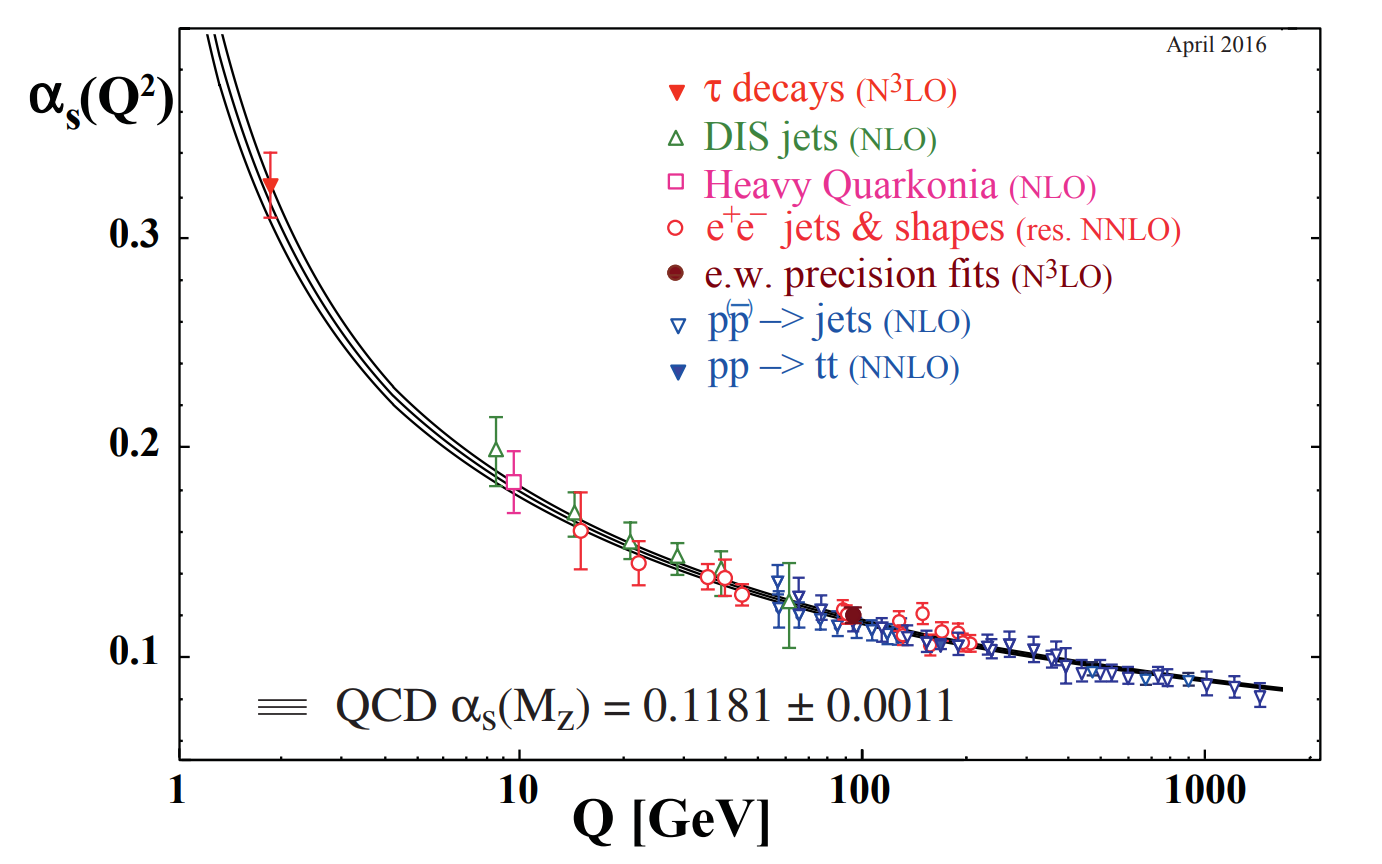
\includegraphics[width=0.6\textwidth]{figures/theory/alphas.png}
    \caption{Running of the QCD coupling strength $\alpha_S$ as a function of length scale.
             Reprinted from Reference~\cite{pdg}.}
    \label{fig:theory:alphas}.
\end{center}
\end{figure}

\subsection{Electroweak interactions}
\label{sec:theory:ew}
The electroweak (EW) sector of the SM refers to the $\SU(2)\times\U(1)$ symmetry group.
While all fermion fields in Table~\ref{tab:theory:fermions} transform under $\U(1)$, only left-handed fermions have non-trivial transformations under $\SU(2)$.
The EW Lagrangian (ignoring particle masses and the Higgs sector for now) is:
\begin{align}
\mathcal{L}_\mathrm{EW} =~
        & i\bar\ell_{iL} \left(\slashed\partial-ig \slashed W^a \tau^a - ig'Y_{\ell_L} \slashed B\right)\ell_{iL} 
      + i\bar q_{iL}^{c} \left(\slashed\partial-ig \slashed W^a \tau^a - ig'Y_{q_L} \slashed B\right)q_{iL}^{c} \nonumber \\
      & + i\bar e_{iR} \left(\slashed\partial-ig'Y_{ e_R}\slashed B\right) e_{iR} 
       + i\bar u_{iR^{c}} \left(\slashed\partial-ig'Y_{u_R}\slashed B\right) u_{iR}^{c} 
       + i\bar d_{iR}^{c} \left(\slashed\partial-ig'Y_{d_R}\slashed B\right) d_{iR}^{c} \nonumber \\ 
      & - \frac{1}{4} W_{\mu\nu}^a W^{a,\mu\nu} - \frac{1}{4} B_{\mu\nu} B^{\mu\nu}  
      \label{eq:theory:lew}
\end{align}
where repeated indices are contracted; the subscript $i$ indexes generations; $g$ and $g'$ are respectively the coupling strengths for $\SU(2)$ and $\U(1)$; $Y$ is the weak hypercharge; $W_\mu^a$ are the three gauge fields corresponding to the generators $\tau^a = \nicefrac{\sigma^a}{2}$ of $\SU(3)$; $B_\mu$ is the gauge field for $\U(1)$; and $W_{\mu\nu}^a$ and $B_{\mu\nu}$ are the field strength tensors for the respective gauge fields.
The covariant derivative can be written as:
\begin{equation}
    D_\mu = \partial_\mu - ig\delta_L W^a_\mu \tau^a - ig' YB_\mu
\end{equation}
where $Y$ is the particle's hypercharge and $\delta_L$ is 1 if the field is in the $\mathbf{2}$ representation of $\SU(2)$ (e.g. left-handed fermions) and 0 otherwise. 

\subsubsection{EW symmetry breaking}
Unlike Equation~\ref{eq:theory:lqcd}, we cannot introduce a quadratic mass term for fermions in Equation~\ref{eq:theory:lew} because $\bar\psi \psi = \psi^\dag_R\psi_L + \psi^\dag_L\psi_R$ is not invariant under $\SU(2)$ rotations.
Spontaneous electroweak symmetry breaking remedies this, as well as provides masses for the gauge fields~\cite{ewsb1,ewsb2,ewsb3,ewsb4,ewsb5,ewsb6}.
A complex scalar doublet $\phi$ (called the complex Higgs field) with $Y_\phi=\nicefrac{1}{2},~\delta_L=1$ is added to the Lagrangian:
\begin{equation}
    \mathcal{L}_\mathrm{EW} \mapsto \mathcal{L}_\mathrm{EW}
            + |D_\mu \phi|^2 + \mu^2|\phi|^2 - \lambda |\phi|^4
    \label{eq:theory:lhiggs}
\end{equation}
We can write the complex doublet as 4 real fields:
\begin{equation}
    \phi = \frac{1}{\sqrt{2}} \left(\begin{matrix} \phi_1 + i\phi_2 \\ \phi_3 + i \phi_4 \end{matrix} \right)
\end{equation}
The two self-interaction terms create a Higgs potential with a degenerate global minimum at \emph{vacuum expectation value} $v \equiv \langle |\phi| \rangle = \sqrt{\nicefrac{\mu^2}{\lambda}}$.
Through gauge rotations, we can fix $\langle\phi_{1,2,4}\rangle = 0$ and, at low energies, expand $\phi_3 = v + H$, where $H$ is the real Higgs field. 
This is the spontaneoous breaking of a symmetry.

By the Nambu-Goldstone theorem~\cite{nambu,goldstone}, these three lost degrees of freedom give rise to three massless bosons. 
The $|D_\mu \phi|$ term couples the complex Higgs field to the gauge bosons:
\begin{align}
    |D_\mu \phi|^2_{\phi = \langle\phi\rangle} &= 
        \frac{v^2}{8} \left[(gW_\mu^1)^2 + (gW^2_\mu)^2 + (g'B_\mu - gW_\mu^3)^2\right] 
\end{align}
The diagonization of this mass term gives 3 massive weak bosons (consuming the 3 massless Nambu-Goldstone bosons) and one massless photon (defining $\tan\theta_w = g'/g$):
\begin{align}
    W^\pm_\mu &\equiv \frac{W_\mu^1 \mp iW_\mu^2}{\sqrt{2}} \nonumber \\ 
    Z_\mu &\equiv \cos\theta_w W_\mu^3 - \sin\theta_w B_\mu \nonumber \\ 
    A_\mu &\equiv \sin\theta_w W_\mu^3 + \cos\theta_w B_\mu
\end{align}
with mass eigenvalues:
\begin{equation}
    m_W = \frac{gv}{2}, \quad m_Z = \frac{v\sqrt{g^2+g'^2}}{2}, \quad m_A = 0
\end{equation}

The remaining $H$ field, which has not been consumed, is the Higgs boson discovered by CMS and ATLAS~\cite{higgsdisc} in 2012.
It has mass $m_H = \sqrt2\mu$.
By expanding $\phi$ around $\langle \phi \rangle$ in Equation~\ref{eq:theory:lhiggs}, we find couplings to the massive gauge bosons:
\begin{gather}
    \frac{m_Z^2}{v} hZ_\mu Z^\mu, \quad \frac{2m_W^2}{v}hW^{+\mu} W^{-}_\mu, \nonumber \\
    \frac{m_Z^2}{2v} h^2 Z_\mu Z^\mu, \quad \frac{m_W^2}{v} h^2 W^{+\mu} W^-_\mu 
\end{gather}
The breaking of the $\SU(2)\times \U(1)$ symmetry leaves behind a local $\U(1)$ symmetry (with gauge boson $A_\mu$), which corresponds to electromagnetism.
Fermions have charge $eQ = e(T_3+Y)$, where $e=g'\cos\theta_w$ and $T_3$ is the third isospin component. 
The $W^\pm$ bosons receive charge $\pm e$.
After symmetry breaking, the actions of the broken gauge groups on fermions are governed by the following Lagrangian terms:
\begin{align}
    \La_\mathrm{EWSB} \supset 
            \sum_f &\left[\bar f\left(i\slashed\partial-eQ_f\slashed A\right) f 
            - \frac{g}{2\sqrt{2}} \bar f_L \left(T^+\slashed W^+ + T^- \slashed W^-\right) f_L\right. \nonumber \\
            &\left.~- \frac{g}{2\cos\theta_w} \bar f\left(g_{Vf} - g_{Af} \right)\slashed Z f \right]
\end{align}
where $f$ are all fermion fields; $f_L = \frac{1}{2}(1-\gamma^5)f$; $g_{V} = T_3- 2Q\sin^2\theta_w$; and $g_{A} = T_3$.

\subsubsection{Fermion masses}
The last piece of the EW Lagrangian is the addition of the fermion masses through Yukawa couplings with the Higgs doublet. 
First, let us add the terms for quark couplings:
\begin{equation}
   \La_\mathrm{EW} \mapsto \La_\mathrm{EW} - y_{ij}^d \bar q_{iL} \phi d_{jR} - y_{ij}^u \bar q_{iL}i\sigma_2 \phi^* u_{uR}i + \hc
\end{equation}
where $\hc$ refers to the Hermetian conjugate of preceding terms; and $y_{ij}^{u,d}$ are the Yukawa matrices for up- and down-type quarks.
Breaking the symmetry and collecting terms proportional to $v$:
\begin{equation}
    -\frac{v}{\sqrt{2}}\left(y_{ij}^d \bar d_{iL}' d_{jR} + y_{ij}^u \bar u_{iL} u_{jR}\right) 
\end{equation}
The mass eigenstates are found by diagonalizing these terms, which are written in terms of the weak eigenstates.
Let us denote the unitary transformations from the mass basis to the weak basis as $U_u$ and $U_d$. 
If we try to write the rest of $\La_\mathrm{EWSB}$ in terms of mass eigenstates, we see that terms of the following form all have trivial transformations:
\begin{gather} 
\bar d' \gamma^\mu d' \mapsto \bar d U_d^\dag \gamma^\mu U_d d = \bar d \gamma^\mu d
\end{gather}
The only non-trivial transformation is in the charged weak interaction:
\begin{align} 
\bar u_L \slashed W^+ d'_L + \bar d'_L W^- u_L &\mapsto 
    \bar u_L \slashed W^+ U_u^\dag U_d d_L + \bar d_L W^- U_d^\dag U_u u_L \nonumber \\
    &\equiv \bar u_L \slashed W^+ V_\mathrm{CKM} d_L + \bar d_L W^- V^\dag_\mathrm{CKM} u_L
\end{align}
where $V_\mathrm{CKM}$ is the Cabibbo-Kobayshi-Maskawa matrix~\cite{ckm1,ckm2}.
It is nearly-diagonal, but with non-zero mixing between the generations. 
The CKM matrix also contains a charge parity (CP) violating phase.
When referring to down-type quarks, we typically refer to the mass eigenstate $d$ as opposed to $d'$.

A similar analysis can be carried out for the lepton sector:
\begin{equation}
   \La_\mathrm{EW} \mapsto \La_\mathrm{EW} - y_{ij}^e \bar \ell_{iL} \phi e_{jR} - y_{ij}^\nu \bar \ell_{iL}i\sigma_2 \phi^* \nu_{uR}i + \hc
\end{equation}
The mixing matrix for leptons is the Pontecorvo-Maki-Nakagawa-Sakata matrix $U_\mathrm{PMNS}$ \cite{pmns}, which relates the weak eigenstates $\nu_e, \nu_\mu,\nu_\tau$ with the mass eigenstates $\nu_1,\nu_2,\nu_3$.
The values of the neutrino masses are known to be non-zero from the observation of neutrino oscillations~\cite{nuosc}.

After EWSB, each fermion mass eigenstate has a mass term and coupling to the Higgs field:
\begin{equation}
    \La_\mathrm{EWSB} \supset \sum_f -\frac{y_f v}{\sqrt{2}} \left( \bar ff + \bar fH f\right)
\end{equation}
where we identify the mass as $m_f = y_f v/\sqrt{2}$. 
Table~\ref{tab:theory:ewsb} summarizes all SM fermions and some of their properties after EWSB.

\begin{table}[]
\begin{center}
    \caption{Summary of the SM fields after electroweak symmery breaking.
             All masses are taken from the global fits compiled by the Particle Data Group~\cite{pdg}.}
    \label{tab:theory:ewsb}
    \begin{tabular}{l|c|c|c|c}
        Name & Symbol & Spin & Mass & $Q_e$  \\  \hline \hline
        gluon & $g^{ab}$ & 1 & 0 & 0 \\   
        photon & $\gamma $ & 1 & 0 & 0 \\   
        $Z$ boson & $Z$ & 1 & 91.2 GeV & 0 \\   
        $W$ boson & $W^{\pm}$ & 1 & 80.4 GeV & $\pm 1$ \\   \hline 
        Higgs boson & $H$ & 0 & 125 GeV & $0$ \\   \hline 
        up quark & $u$ & $\nicefrac{1}{2}$ & $2.2$ MeV & $\nicefrac{2}{3}$    \\   
        down quark & $d$  & $\nicefrac{1}{2}$ & $4.7$ MeV  & $-\nicefrac{1}{3}$  \\   
        charm quark & $c$  & $\nicefrac{1}{2}$ & $1.28$ GeV  & $\nicefrac{2}{3}$  \\   
        strange quark & $s$  & $\nicefrac{1}{2}$ & $95$ MeV  & $-\nicefrac{1}{3}$  \\   
        top quark & $t$  & $\nicefrac{1}{2}$ & $173$ GeV  & $\nicefrac{2}{3}$  \\  \hline
        bottom quark & $b$  & $\nicefrac{1}{2}$ & $4.18$ GeV  & $-\nicefrac{1}{3}$  \\   
        electron neutrino  & $\nu_e$  & $\nicefrac{1}{2}$ & $-$  & $0$  \\   
        electron  & $e$  & $\nicefrac{1}{2}$ & $511$ keV  & $-1$  \\   
        muon neutrino  & $\nu_\mu$  & $\nicefrac{1}{2}$ & $-$  & $0$  \\   
        muon  & $\mu$  & $\nicefrac{1}{2}$ & $105$ MeV  & $-1$  \\   
        tau neutrino  & $\nu_\tau$  & $\nicefrac{1}{2}$ & $-$  & $0$  \\ 
        tau  & $\tau$  & $\nicefrac{1}{2}$ & $178$ GeV  & $-1$  \\   
    \end{tabular}
\end{center}
\end{table}

\section{Dark matter}

While the SM is incredibly powerful at predicting the outcomes of many laboratory experiments, there are certain major phenomena it cannot predict:
\begin{itemize}
    \item There is not yet a complete formulation of \emph{quantum gravity}, folding in general relativity~\cite{gr}.
    \item The observed \emph{matter/antimatter asymmetry} in the universe cannot be explained by the SM's CP violation and (predicted) baryon number of violation. 
          Additional CP and $B$ violating interactions must exist.
    \item \emph{Neutrino masses} are not completely determined by the SM. 
            While a mass term can be written down as in Section~\ref{sec:theory:ew}, it does not exclude a Majorana mass term for right-handed neutrinos. 
            Nor does it explain the observed range of masses $m_\nu/m_t \lesssim 10^{-15}$. 
    \item An explanation of \emph{dark energy} accounting for $\sim 68\%$ of the universe's energy budget, suggested by measurements of the CMB, galaxy clusters, supernovae, and other measurements of the universe expansion rate~\cite{darkenergy}.
    \item An explanation of \emph{dark matter} accounting for $\sim 27\%$ of the universe's energy budget, suggested by measurements of galactic rotation curves, the CMB, and gravitational lensing~\cite{pdg,dm1,dm2,dm3}.
\end{itemize}
In this thesis, we describe tests of certain extensions of the SM which add candidate fields for dark matter (DM). 

\subsubsection{Astrophysical evidence}
All known evidence of DM arises from gravitational measurements.
One of the oldest observations is that of galactic rotational curves.
The rotational velocities of stars and hydrogen clouds are measured in galaxies, as a function of distance from the center of the galaxy.
It is found that the velocity increases as a function of $r$, eventually reaching a plateau that extends well past the bulk of the visible mass of the galaxy.
This implies the existence of a massive dark halo that encompasses the galaxy.
Indeed, the observed rotational curves $v(r)$ are well-described by a 3 component fit: the visible disk, a gas cloud, and a dark halo. 
Two galaxies are shown in Figure~\ref{fig:theory:dm_rot}, and it is clear that a non-zero DM component is needed to describe the data.

\begin{figure}[]
\begin{center}
    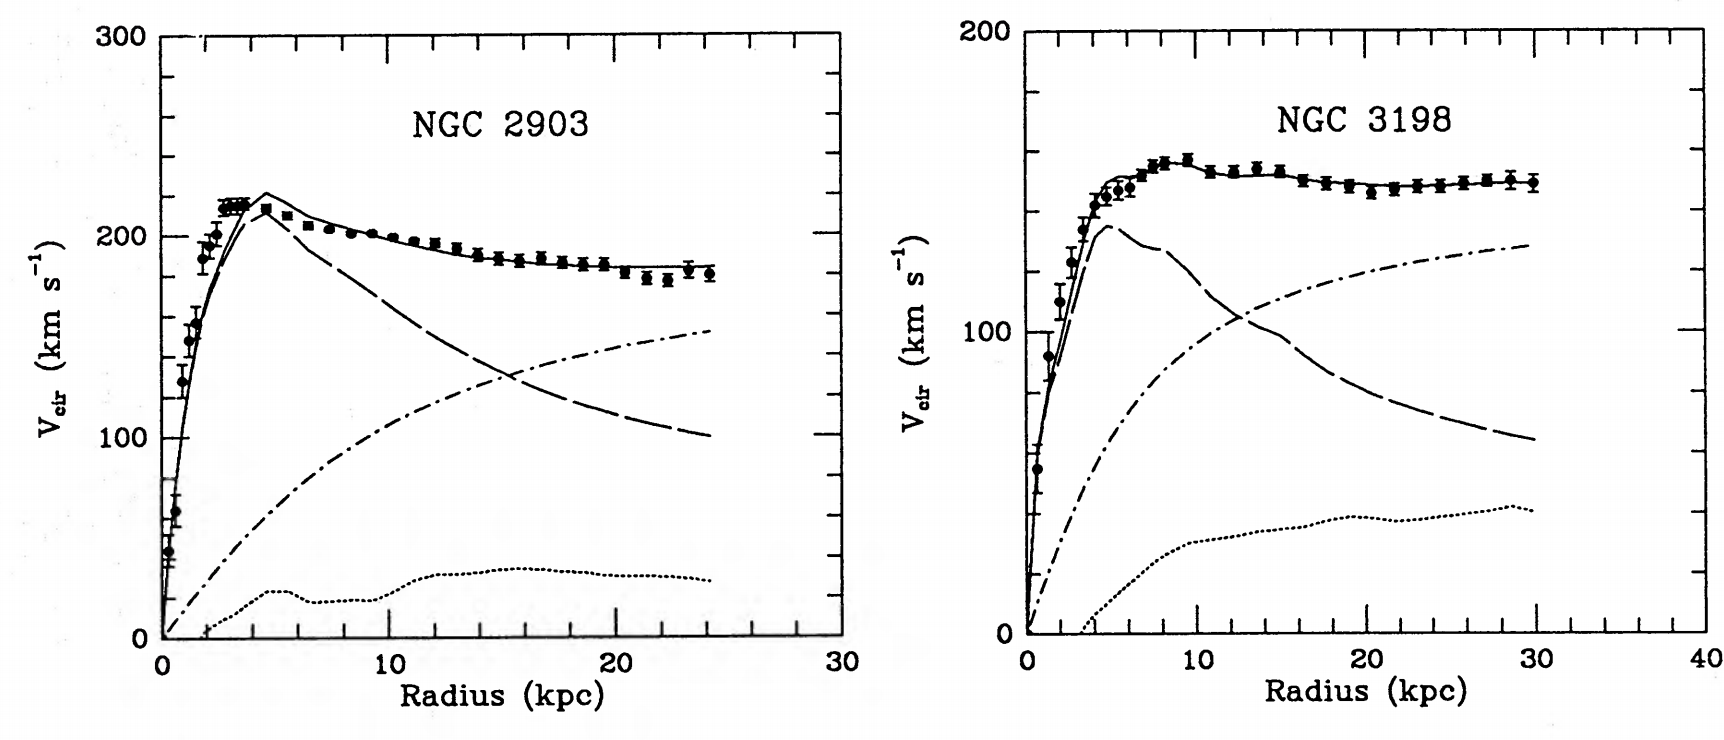
\includegraphics[width=0.7\textwidth]{figures/theory/dm_rot.png}
    \caption{Observed and fitted galactic rotational curves for two galaxies.
             The total fit (solid line) has three components: visible (dashed), gas clouds (dotted), and DM (dash-dotted). 
             Reprinted from Reference~\cite{dmrot}.}
    \label{fig:theory:dm_rot}
\end{center}
\end{figure}

An orthogonal piece of evidence comes from measuring anisotropies in the cosmic microwave background (CMB).
The CMB is the remnant of photons after they decoupled from matter in the early universe.
The temperature spectrum of the CMB is isotropic to one part in $10^5$, and the anisotropies are driven by matter anisotropies at the time of decoupling.
The power spectrum of the temperature anisotropies is modified when there are two matter populations (SM and DM) as opposed to one (just SM), especially when the two populations interact with each other (via gravity) but one does not interact with photons (DM).
Figure~\ref{fig:theory:planck} shows the power spectrum measured by the Planck experiment~\cite{planck}, compared to the best-fit $\Lambda$ Cold Dark Matter ($\Lambda$CDM) model.

\begin{figure}[]
\begin{center}
    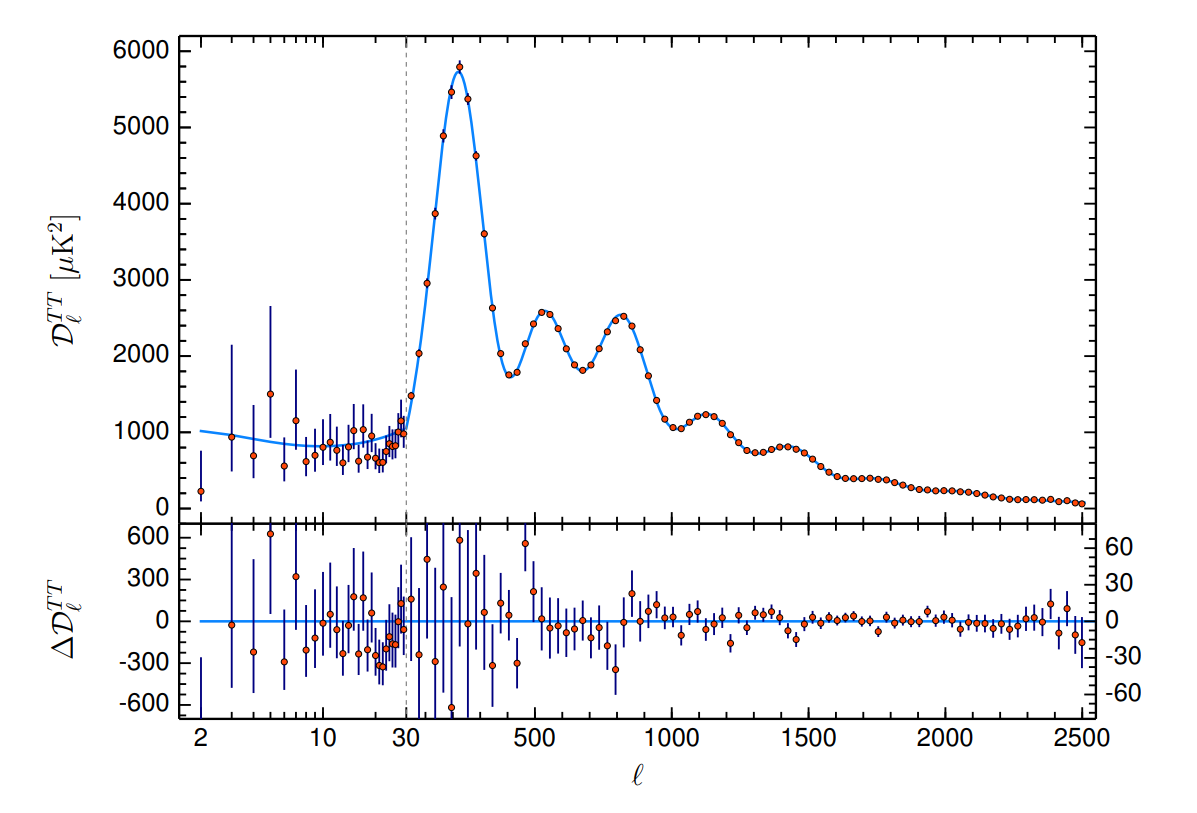
\includegraphics[width=0.7\textwidth]{figures/theory/planck.png}
    \caption{Temperature anisotropy power spectrum of the CMB, as measured by Planck.
             Reprinted from Reference~\cite{planck}.}
    \label{fig:theory:planck}
\end{center}
\end{figure}

This is hardly an exhaustive list of DM evidence.
Other observations include gravitational lensing, cluster collisions, and large-scale structure formation~\cite{dm1,dm2}.

\subsubsection{DM candidates}

The \emph{relic density} is the current density of a field that fell out of thermodynamic equilibrium with other fields as the universe expanded.
This occurs as the rate of expansion of the universe outpaces the mean particle velocity $v$ (correlated with the temperature $T$) and the cross sections for annihilation and production of the field.
This decoupling of the field is known as \emph{freeze-out}.
The relic density is defined:
\begin{equation}
    \Omega \cdot h^2 = \frac{\rho}{\rho_c} \cdot \frac{H_0}{100\text{ km/s/Mpc}}
\end{equation}
where $\rho$ is the energy density of the field, $\rho_c$ is the critical total energy density of flat spacetime, and $H_0=73$ km/s/Mpc is the Hubble constant.
If $\sigma_A$ is the annihilation cross section and the field is non-relativistic at freeze-out, then a very simplified approximation~\cite{dm1} is:
\begin{equation}
    \Omega h^2 = \frac{10^{-27}\mathrm{cm}^3\mathrm{s}^{-1}}{\langle \sigma_A v\rangle}
    \label{eq:theory:relic}
\end{equation}
Planck~\cite{planck} measures the relic densities of baryonic and dark matter to be:
\begin{equation}
    \Omega_b h^2 = 0.02237 \pm 0.0015, \quad \Omega_\mathrm{DM} h^2 = 0.1200 \pm 0.0012
\end{equation}

As a first candidate, suppose we introduce a fermion $\chi$ is a particle with mass $m_\chi\sim100$ GeV.
Further suppose that it has an interaction with the SM through a new current, and the cross section for the effective four-point interaction $\chi \bar\chi\rightarrow f\bar f$ (for some SM fermion $f$) is proportional to $g^4_\chi$, where $g_\chi \sim g \sim 0.6$.
The relic density for such a particle would be $\Omega_\chi h^2 \sim 0.1$, which is quite close to the needed density.
A \emph{Weakly-Interacting Massive Particle} (WIMP) such as $\chi$ therefore makes a good DM candidate.
This coincidence is known as the \emph{WIMP miracle}.
It should be noted that the definition of a WIMP is fairly loose.
All models considered in these results contain at least one particle falls under the umbrella of a WIMP, but the models themselves are quite diverse.

The obvious SM candidate for DM are neutrinos, as they are known to be non-interacting and massive.
However, constraints on the neutrino mass restrict $\Omega_\nu h^2 \leq 0.0062$~\cite{pdg}, which is far too small to entirely account for the observed phenomena. 
Sterile neutrinos (neutrinos that participate in oscillations but do not couple to the $Z$ boson) remain a viable DM candidate, above a mass of 10 keV.
A proposed solution to the strong CP problem is the addition of a scalar \emph{axion} field.
While axions can have couplings to photons, those interactions would be sufficiently weak for an axion to remain \emph{dark} in the sense of DM.
Many other DM candidates have been proposed as well (some of which fall under the generic WIMP umbrella), and this is not an exhaustive list.

\subsubsection{Non-collider WIMP searches}

Each class of DM models has dedicated experimental signatures, and therefore dedicated experiments to search for them.
Here, we focus on searches sensitive to WIMPs, as these are most relevant for the results in this thesis.

The philosophy of collider DM searches is to produce DM in the laboratory and directly or indirectly detect it.
Non-collider searches rely on DM that is present somewhere in the universe and look for its interaction with SM particles.

\emph{Indirect detection} experiments look for the annihilation process $\chi\bar\chi\rightarrow X$, where $X$ is one or more SM particles.
The Alpha Magnetic Spectrometer (AMS-02) searches for excess positrons in the cosmic ray flux, arising from $X=e^+e^-$ final states~\cite{ams}. 
Similarly, $\gamma$ ray data from the Fermi Large Area Telescope (Fermi-LAT) is used to look for final states which include high-energy photons~\cite{fermilat}.
As an example, the 95\% CL exclusion from Fermi-LAT is shown in Figure~\ref{fig:theory:fermilat}.
The exclusion is drawn as a function of $m_\chi$ and $\langle \sigma_A v\rangle$, as the Fermi-LAT analysis is directly dependent on the annihilation rate.
Also shown is an exclusion from a search conducted by the CMS experiment at the LHC, looking for the process $pp\rightarrow \chi+$jet and assuming a pseudoscalar mediator connecting the DM and SM sectors~\cite{monojet}.

\begin{figure}[]
\begin{center}
    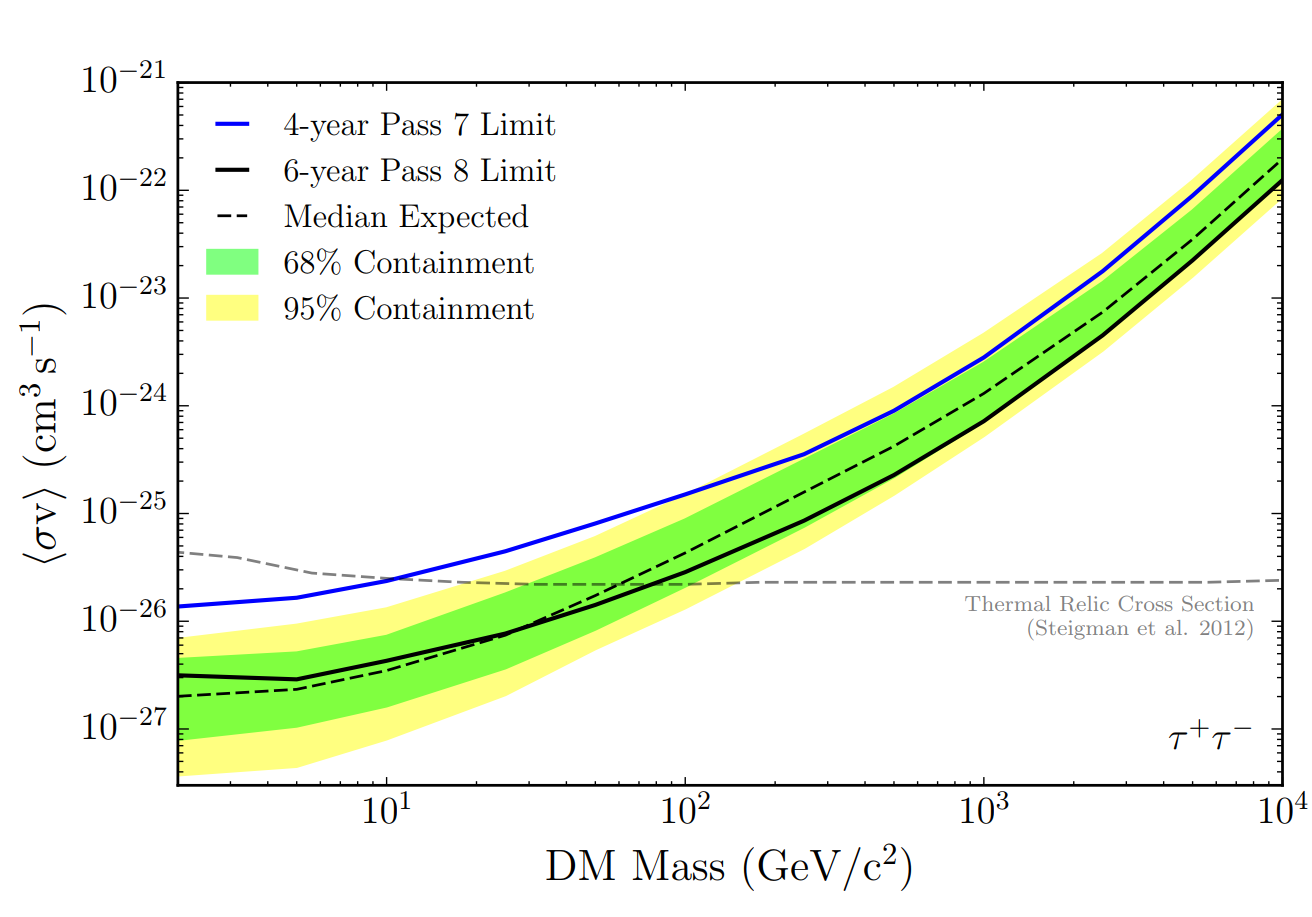
\includegraphics[width=0.5\textwidth]{figures/theory/fermilat.png}
    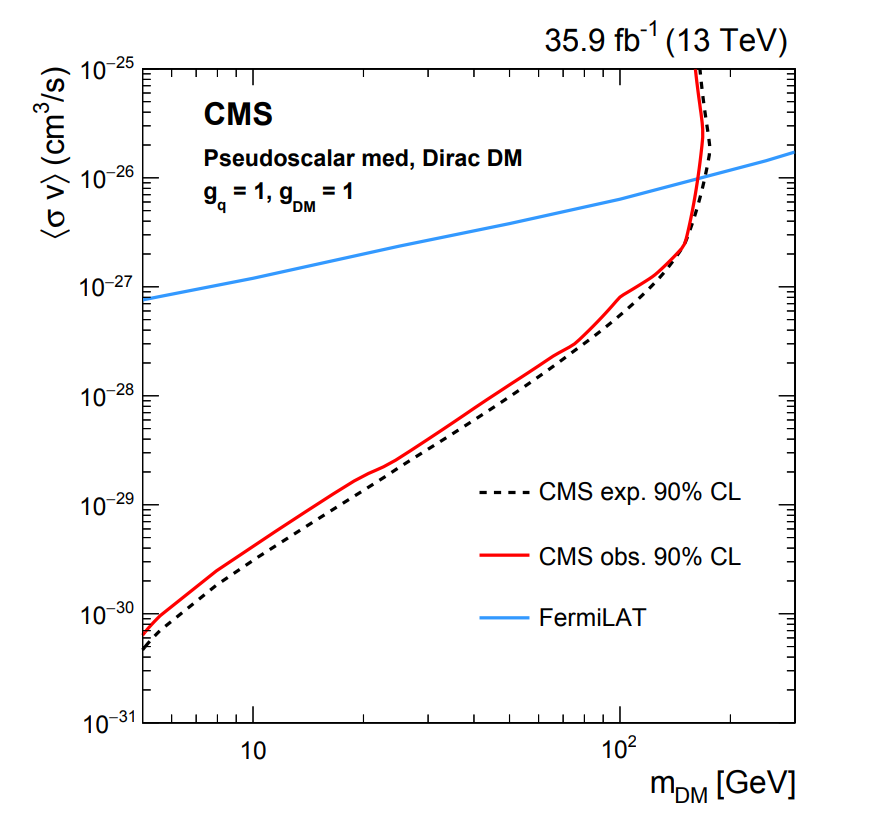
\includegraphics[width=0.4\textwidth]{figures/theory/monojet.png}
    \caption{Excluded WIMP hypotheses as a function of $m_\chi,\langle\sigma v\rangle$ from Fermi-LAT (left) and compared to CMS (right).
             Reprinted from Reference~\cite{fermilat} (left) and Reference~\cite{monojet} (right).}
    \label{fig:theory:fermilat}
\end{center}
\end{figure}

\emph{Direct detection} experiments typically contain a large volume of instrumented material that has a large cross section for interaction with WIMPs.
An example is the Large Underground Xenon (LUX) experiment~\cite{lux}, a two phase (liquid and gas) xenon detector.
LUX searches for scintillation photons and additional electrons emitted from DM-nucleus interactions.
Xenon is chosen because heavy nuclei have larger cross sections for \emph{spin independent} DM interactions.
In this context, spin independent refers to any interaction mediated by a scalar or vector current (i.e. there is no coupling to the spin of the DM or nucleon). 
Figure~\ref{fig:theory:lux} compares the exclusions of LUX to other direct detection experiments.
The results are presented as a function of the natural quantities for direct detection: $m_\chi$ and $\sigma(\chi N \rightarrow \chi N)$.
Also shown is the exclusion limit from the CMS invisible Higgs search, which is described in Chapter~\ref{sec:vbf}.

\begin{figure}[]
    \begin{center}
        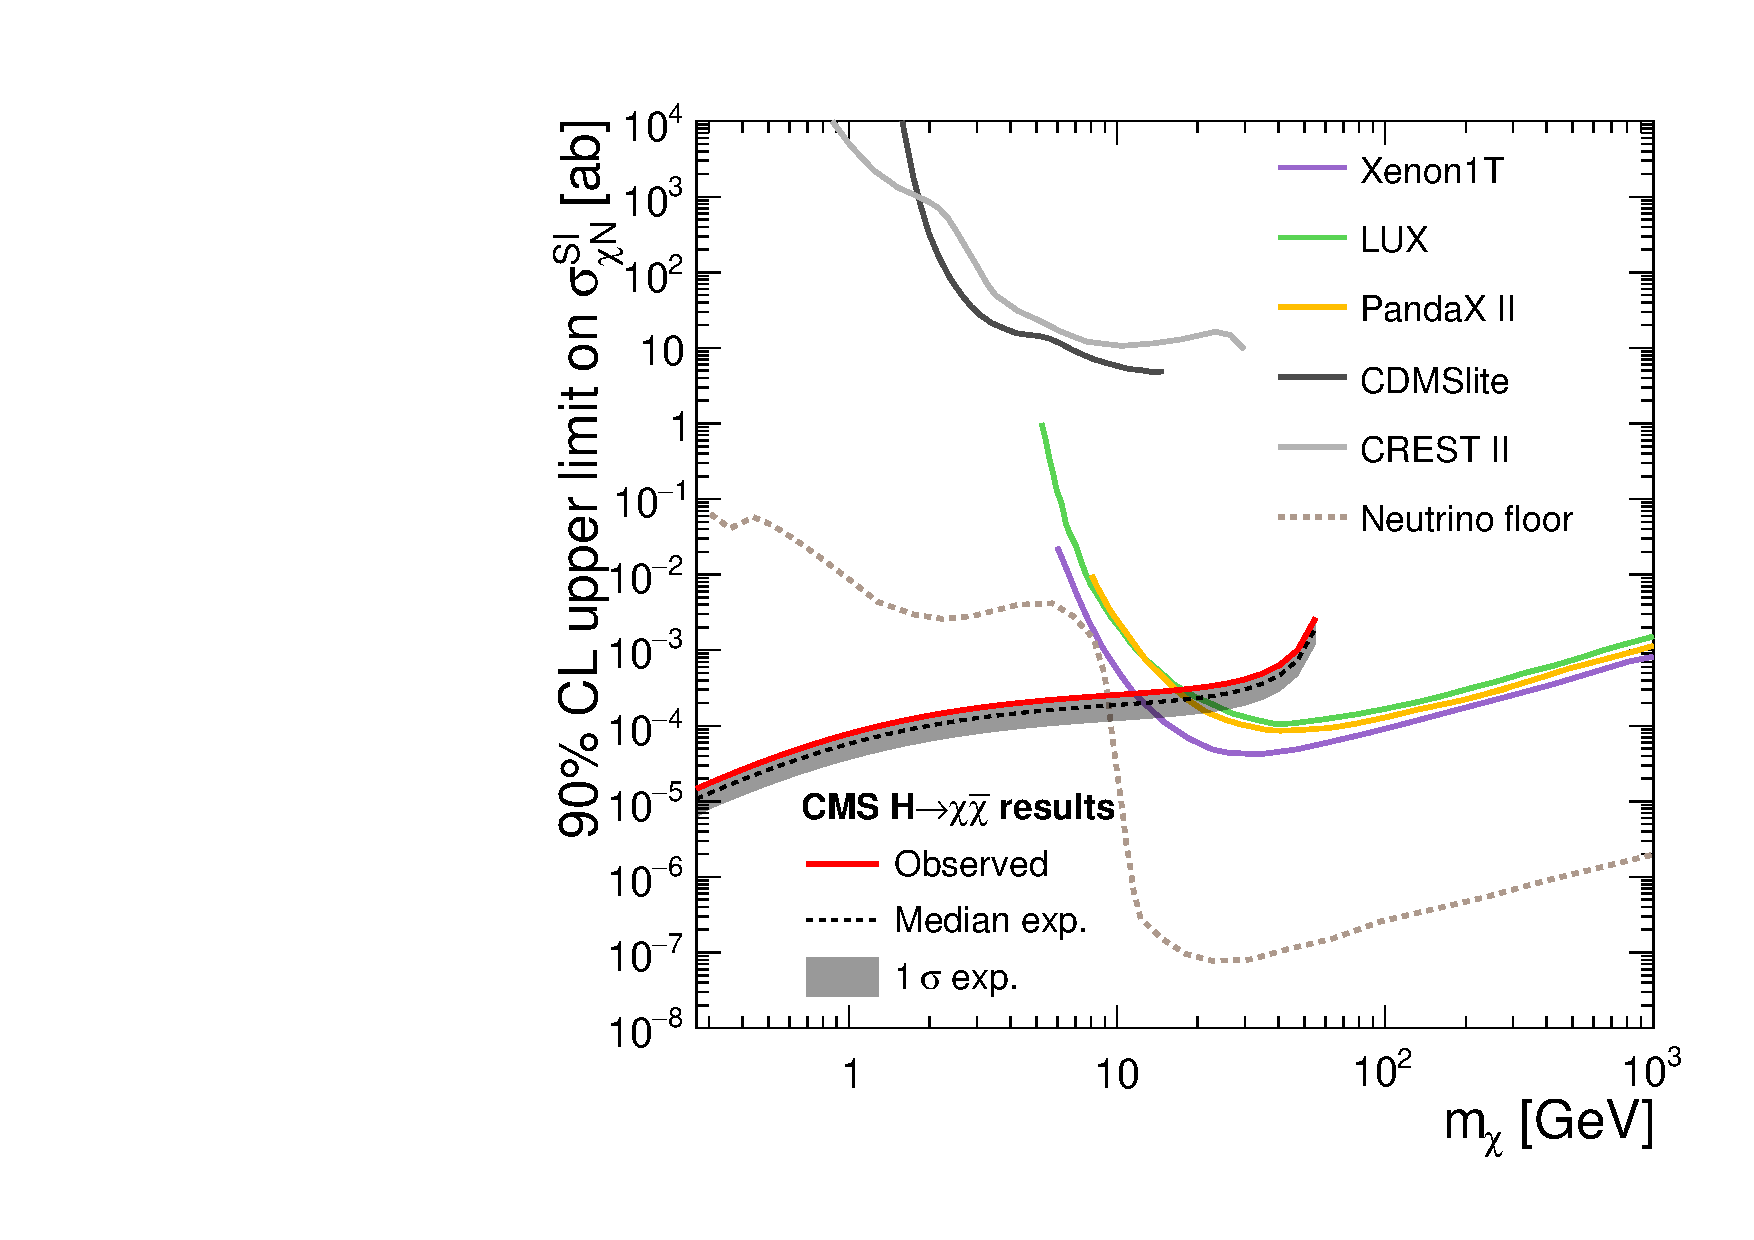
\includegraphics[width=0.5\textwidth]{figures/vbf/fits/dd.pdf}
        \caption{Comparison of various direct detection experiments' sensitivity to WIMP models and the sensitivity of the CMS invisible Higgs search.
                 Details of the CMS curve are presented in Chapter~\ref{sec:vbf}.}
        \label{fig:vbf:lux}
    \end{center}
\end{figure}

The results presented in this section suggest that collider searches have complementary sensitivity for certain DM hypotheses, typically at low masses.
The searches described in this thesis target those models, as well as exotic models to which standard direct and indirect detection experiments have very little sensitivity.

\section{LHC phenomenology}

The Large Hadron Collider collides protons at a center of mass energy $\sqrt{s} = 13$ TeV.
Section~\ref{sec:cms:lhc} provides an overview of the LHC machine.
In this section, we describe the methods used to make predictions of observables at the LHC.
These observables typically take the form of differential cross sections $\di\sigma(pp\rightarrow X)/\di\Theta$, where $X$ is some interesting final state with $N$ particles and $\Theta$ is a set of interesting kinematics.
The differential element of the general cross section for $2\rightarrow N$ processes is:
\begin{equation}
\di\sigma(ab\rightarrow \{c_i\}) = 
    \frac{1}{2s} \left(\prod_i \dfrac{\mathrm{d}^3p_i}{(2\pi)^3} \frac{1}{2E_i}\right) 
        \cdot (2\pi)^4 \delta^4\left(k_a + k_b - \sum_i p_i\right) 
        \cdot \left|\Ma(ab\rightarrow \{c_i\})\right|^2
        \label{eq:theory:2n}
\end{equation}
where $k_a,k_b$ are the incoming momenta; $\{p_i\}$ are the outgoing momenta; and $\Ma$ is the matrix element of this reaction.

Hadron collisions do not have two-particle initial states, but rather two composite particles containing partons with varying momenta. 
The general cross section for $pp\rightarrow X$ is~\cite{tasi009}:
\begin{equation}
\di\sigma(pp\rightarrow X(\Theta)) = 
    \sum_{a,b} \int \mathrm{d}x_a \mathrm{d}x_b 
    ~f_a(x_a,\mu_F) f_b(x_b,\mu_F) 
    \cdot \di\sigma(ab\rightarrow\{c_i\}) 
    \cdot D(\{c_i\}\rightarrow X(\Theta))
    \label{eq:theory:master}
\end{equation}
The sum over $a,b$ refers to summing over partons in the initial state.
The momentum fractions of the partons, $x_{a,b}$, follow parton distribution functions (PDFs) $f_{a,b}$ that depend on the particle species $a$ and $b$. 
We then define an intermediate state $\{c_i\}$ which evolves into the final state $X(\Theta)$.
That is, the process $ab\rightarrow X$ is split into $ab\rightarrow \{c_i\} \rightarrow X$.
The definition of $\{c_i\}$ is not unique, but is chosen such that the process $ab\rightarrow\{c_i\}$ can be analyzed perturbatively.
The non-perturbative aspects of evolution to the final state (soft or collinear radiation) will be analyzed separately. 
The matrix element for the first step (\emph{hard scattering}) is computed perturbatively and turned into a cross section by means of Equation~\ref{eq:theory:master}.
Other heuristic methods are used to deal with the second step (\emph{parton shower} (PS)), encoded in the \emph{fragmentation function} $D$. 

The ability to partition the calculation into perturbative (hard scattering) and non-perturbative (PDF and parton shower) components follows from the collinear factorization theorem~\cite{fact}.
The factorization depends on an arbitrary energy scale $\mu_F$, which defines a lower bound for interactions considered part of the hard scattering. 
The remainder of this section discusses the use of Monte Carlo (MC) methods to simulate these three factors: $f$, $\Ma$, and $D$.

\subsection{Parton distribution functions}
The analytic behavior of PDFs as a function of the factorization scale is governed by the DGLAP evolution equation~\cite{dglap1,dglap2,dglap3}:
\begin{gather}
    \mu_F \frac{\di}{\di\mu_F} f_a(x_a,\mu_F) = \frac{\alpha_S}{\pi} \int_x^1 \frac{\di y}{y} f_a(y,\mu_F) P_{qq} \left(\frac{x}{y}\right) \\
    \text{where } P_{qq}(z) = \frac{4}{3}\left[\frac{1+z^2}{1-z}\right]_+ + 2\delta(1-z) \nonumber 
    \label{eq:theory:dglap}
\end{gather}
The computation of $f_a$ for a fixed scale cannot be done analytically.
Instead, data from many experiments are used to fit a parameterization, as is done by the NNPDF collaboration~\cite{nnpdf}.
Results presented in this thesis use the NNPDF3.0 PDF set.

\subsection{Hard scattering}

Monte Carlo generators simulate Equation~\ref{eq:theory:2n} by sampling events with probability proportional to the phase space and matrix element.
The dedicated MC generators used in this result are MadGraph5~\cite{mg5,fxfx} and Powheg2~\cite{powheg}.
Both generators can simulate to leading order (LO) in EW vertices and up to next-to-leading order (NLO) in QCD vertices.
Finally, the PS model Pythia8.2~\cite{pythia} (discussed in the next section) can also generate certain hard scattering processes at LO in QCD.

MC generators also generate additional partons from initial and final state radiation as part of the hard scattering.
These quarks, gluons, and photons can be highly energetic in events with large $q^2$, and so it is necessary to compute them as part of the hard scattering matrix element.  
It should be noted that, while NLO event generation is always preferable, it comes with two costs: (a) being able to generate fewer additional partons and (b) additional computational time.
We will use LO simulation for processes which have large cross sections and in which additional parton spectra are important.
Table~\ref{tab:theory:sim} provides a summary of the MC generators and orders used in these results.

\begin{table}[]
\begin{center}
    \caption{Summary of MC generators used for each SM and signal process.
             Note that the $V$+jet processes have two entries each in this table, at different QCD orders.
             Both will be used to improve the prediction accuracy.}
    \label{tab:theory:sim}
    \begin{tabular}{c|c|c|l}
        $pp\rightarrow X$ & Generator & NLO in QCD? & Notes \\ \hline \hline
        $t\bar{t}$ & Powheg & \cmark \\ 
        $t$, $tW$, $tZ$ & Powheg & \cmark \\ 
        \hline
        $ZZ,~WZ,~WW$ & Pythia &  \\ 
        \hline
        $Z$ (+0,1 partons) & MG  & \cmark  \\ 
        $W$ (+0,1 partons) & MG  & \cmark \\ 
        $\gamma$ (+0,1 partons) & MG  & \cmark  \\ 
        \hline
        $Z$ (+0,1,2,3 partons) & MG  &  \\ 
        $W$ (+0,1,2,3 partons) & MG  &  \\ 
        $\gamma$ (+0,1,2 partons) & MG  &  \\ 
        Multijet & MG && Jets defined in Section~\ref{sec:theory:ps} \\
        \hline
        Resonant DM & MG && See Chapter~\ref{sec:monotop} \\ 
        FCNC DM & MG &\cmark& See Chapter~\ref{sec:monotop} \\ 
        VBF $\hinv$ & Powheg && See Chapter~\ref{sec:vbf} \\ 
    \end{tabular}
\end{center}
\end{table}

\subsection{Parton shower}
\label{sec:theory:ps}
Suppose we know $\di\sigma(ab\rightarrow \{c_i\})$ and would like to know $\di\sigma(ab\rightarrow\{c_i\}j)$, where $j$ is radiated from one of the $c_i$ in the soft and/or collinear limit.
Such ``splittings'' include:
\begin{gather}
    q\rightarrow qg, \quad g\rightarrow qq, \quad g\rightarrow gg, \nonumber \\ 
        f\rightarrow f\gamma, \quad \gamma\rightarrow ff 
\end{gather}
Define $z$ to be the fraction of energy kept by the parent parton and $\theta$ to be the opening angle between $c_i$ and $j$. 
For QCD splittings, the cross section can be written (at LO):
\begin{equation}
    \di\sigma(ab\rightarrow\{c_i\}j) =
        P_{c_i \rightarrow c_i j} (z) 
        \cdot \frac{\alpha_S}{2\pi} 
        \cdot \frac{\di\theta}{\theta} 
        ~\di z
        ~\di\sigma(ab\rightarrow\{c_i\})
\end{equation}
where $P_{c_i\rightarrow c_i j}$ are \emph{splitting functions} analogous to the ones that arise in the DGLAP evolution (Equation~\ref{eq:theory:dglap}).
As an example, the splitting function for $q\rightarrow qg$ is~\cite{pythia}:
\begin{equation}
    P_{q\rightarrow qg} = \frac{4}{3} \frac{1+z^2}{1-z}
\end{equation}

It should be noted that this cross section grows as $\theta\rightarrow 0$ and $z\rightarrow 1$, i.e. soft and collinear splittings.
That is, if a bare quark is produced in an event, it will produce many soft and collinear gluons (which in turn can split to $qq$ and $gg$) prior to hadronization.
This iterative process is known as the $\emph{parton shower}$.
As the width of the parton shower nears $1/\Lambda_\mathrm{QCD}$, the partons will hadronize, preventing further splitting.
These hadronic endpoints of the shower reach the detector and appear as collimated sprays of hadrons (\emph{jets}).
The reconstruction of jets is described in detail in Section~\ref{sec:cms:jets} and Chapter~\ref{sec:jets}. 

PS models simulate the shower and hadronization processes.
The results in this thesis use Pythia8.2~\cite{pythia} which employs the Lund string model~\cite{lund} to simulate hadronization.

\chapter{The CMS experiment at the LHC}
\label{sec:cms}

\section{The Large Hadron Collider}

The Large Hadron Collider (LHC)~\cite{lhcjinst}\footnote{Unless otherwise specified, all technical specifications of the LHC are derived from Reference~\cite{lhcjinst}} is a circular particle accelerator, 27 km in circumference and between 40 and 175 m below the surface of the French-Swiss border. 
Designed to collide protons at a maximum center-of-mass energy $\sqrt{s} = 14$ TeV, the LHC has delivered collisions at $\sqrt{s}=7,8$ TeV (Run 1) and $\sqrt{s} = 13$ TeV (Run 2); the target energy $\sqrt{s} = 14$ TeV will be reached in Run 3. 
In addition to protons, the LHC accelerates and collides heavy nuclei (Pb and Xe) at lower values of $\sqrt{s}$. 
In this thesis, we focus exclusively on data recorded from proton collisions during Run 2. 

\begin{figure}[]
    \begin{center}
        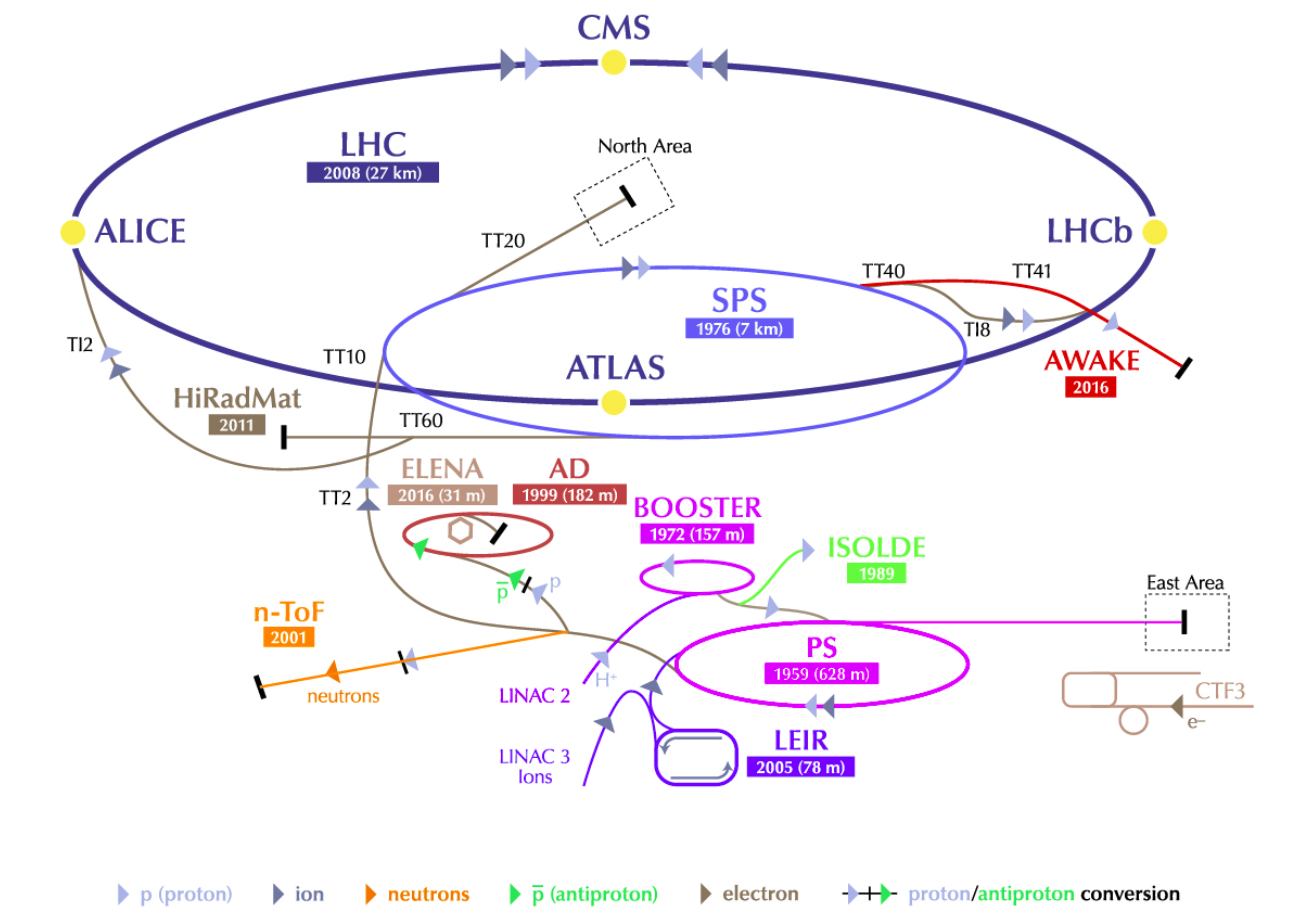
\includegraphics[width=0.8\textwidth]{figures/cms/lhc.png}
        \caption{Diagram of the CERN accelerator complex.
                 The LHC (dark blue) is fed protons (and heavy ions) by a chain of intermediate accelerators, beginning with LINAC2 (dark pink).i
                 Reprinted from Reference~\cite{lhcpic}. 
                    }
        \label{fig:cms:lhc}
    \end{center}
\end{figure}

Protons are brought to the LHC by the multi-stage process~\cite{lhctdr3} depicted in Figure~\ref{fig:cms:lhc}.
Hydrogen atoms are stripped of electrons and accelerated by LINAC2 (a linear accelerator) to a kinetic energy of $50$ MeV.
LINAC2 then feeds the protons into the Booster ring (final energy of $1.4$ GeV), followed by the Proton Synchrotron ($26$ GeV).
From the PS, the protons are injected into the Super Proton Synchrotron ($450$ GeV).
Protons exit the SPS and enter the LHC at one of two places, corresponding to two different beams traveling in opposite directions.
The two beams intersect in eight places along the LHC, four of which are instrumented by a detector experiment: CMS, ATLAS, LHCb, and ALICE. 

Each proton beam in the LHC is accelerated by eight superconducting cavities exerting radio frequency longitudinal (i.e. parallel to beam direction) electric fields with a frequency of $400$ MHz,
The maximum RF voltage seen by each beam is 16 MV per revolution.
The physical and temporal design of the RF system creates bunches of protons (corresponding to nodes of the oscillating field) approximately 7.5 cm in length and separated by 25 ns. 
Superconducting NbTi dipole magnets bend the two proton beams in opposite directions as they travel around the ring. 
Each of the 1232 dipoles is 14 m long and exerts a transverse $B$ field between $0.54$ and $8.33$ T.
To achieve such high $B$ fields, the magnets are cooled to 2 K by superfluid helium.
In addition, a number of quadrupole magnets are used to focus and match the beams between the dipoles\footnote{Full details on the various quadrupoles can be found in Table 3.7 of Reference~\cite{lhcjinst}.}.

In addition to the center-of-mass energy $\sqrt{s}$, the other figure of merit is the number of events producing interesting physics processes, which is defined as:
\begin{equation} 
    N(pp\rightarrow X) = \int dt L \sigma(pp\rightarrow X)
\end{equation}
where $\sigma$ is the cross section of the relevant process and $L$ is the instantaneous luminosity of the LHC. 
The cross section is fixed by nature, and so increasing the luminosity is the only handle to increase $N$. 
The instantaneous luminosity of two Gaussian beams is given by~\cite{lhcjinst}:
\begin{equation}
    L = \frac{N_b^2 n_b f_\mathrm{rev} \gamma F}{4\pi\epsilon \beta^*}
\end{equation}
where:
\begin{itemize}
    \item[$N_b$ $=$] particles per bunch
    \item[$n_b$ $=$] bunches per beam 
    \item[$f_\mathrm{rev}$ $=$] frequency of revolution 
    \item[$\gamma$ $=$] $E/m$ of beam 
    \item[$\epsilon$ $=$] emittance of beam 
    \item[$\beta^*$ $=$] beta function at collision point 
    \item[$F$ $=$] factor accounting for beam intersection geometry
\end{itemize}
The instantaneous luminosity evolves as a function of time, primarily due to $n_b$ and $N_b$ being modified by collisions.
The total integrated luminosity after time $T$ is:
\begin{equation}
    L_\mathrm{int} = \int_0^T dt L(t) = L(0) \tau_L \left(1 - e^{-T/\tau_L}\right)
\end{equation}
where $\tau_L \approx 15$ h is the characteristic beam loss timescale and $L(0)$ is the instantaneous luminosity at $T=0$.
The LHC is designed to deliver $L(0) \sim \mathcal{O}(10^{34})$ cm$^{-2}$s$^{-1}$. 
Figure~\ref{fig:cms:lumi} shows the total luminosity delivered by the LHC and recorded by CMS during the 2016 portion of Run 2. 

\begin{figure}[]
    \begin{center}
        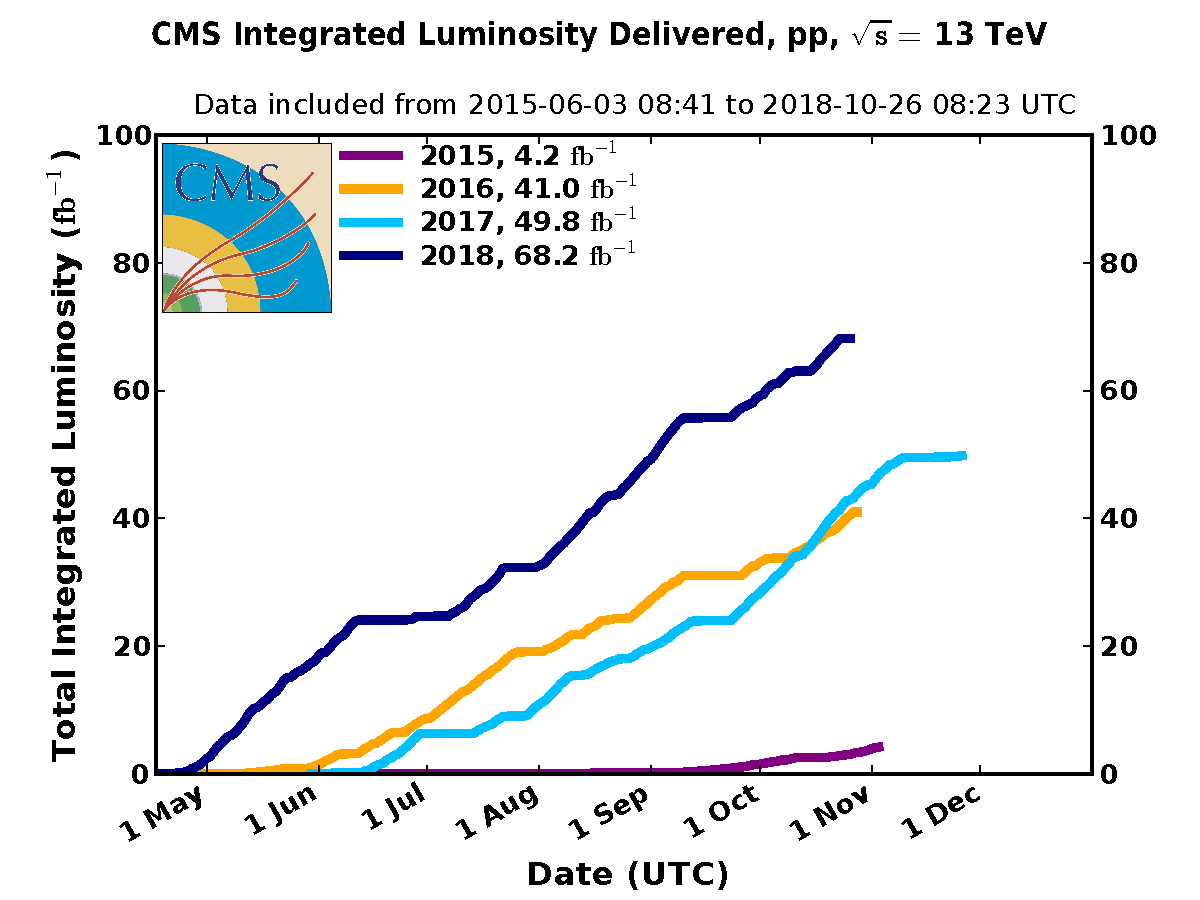
\includegraphics[width=0.5\textwidth]{figures/cms/lumi.pdf}
        \caption{Integrated luminosity of the LHC during proton collisions during the 2016 data-taking period~\cite{lumitwiki}.}
        \label{fig:cms:lumi}
    \end{center}
\end{figure}

\section{The Compact Muon Solenoid}

The Compact Muon Solenoid (CMS)~\cite{cmsjinst} is one of two general purpose LHC detectors (the other being ATLAS).
It is designed to detect and measure stable hadrons, photons, electrons, and muons produced in proton and ion collisions at LHC interaction point 5. 
From these event descriptions, a number of physics processes can be probed, including SM measurements~\needcite, BSM searches~\needcite, and the discovery of the Higgs boson~\needcite. 
In what follows, we will use the $(r,\phi,\eta)$ coordinate system with respect to the $z$ axis:
\begin{itemize}
    \item[$z = $] distance along beam axis, with $z=0$ defined to be at the center of the detector
    \item[$r = $] distance from the $z$ axis
    \item[$\phi = $] azimuthal angle in the plane orthogonal to the $z$ axis
    \item[$\eta = $] pseudorapidity $(-\log\nicefrac{\theta}{2}$), with respect to the polar angle $\theta$ 
\end{itemize}
In this coordinate system, we define $x$ and $y$ to lie in the plane perpendicular to $z$, with $x$ pointing from the center of the detector to the center of the LHC.
As with the pseudorapidity, it is convenient to use quantities invariant under $z$-boosts, and so we define the transverse momentum:
\begin{equation}
    \vec{p}_\mathrm{T} = \left(\begin{matrix} p_x \\ p_y \end{matrix}\right)
\end{equation}
We will frequently make use of the magnitude of this vector, $\pt$. 
CMS can detect collision products that are within the fiducial volume of $0 \leq \phi < 2\pi$ and $-5 \leq \eta\leq 5$. 
Several detector subsystems (Figure~\ref{fig:cms:cms}) are used to identify and reconstruct muons, electrons, photons, and charged and neutral hadrons. 

\begin{figure}[]
    \begin{center}
        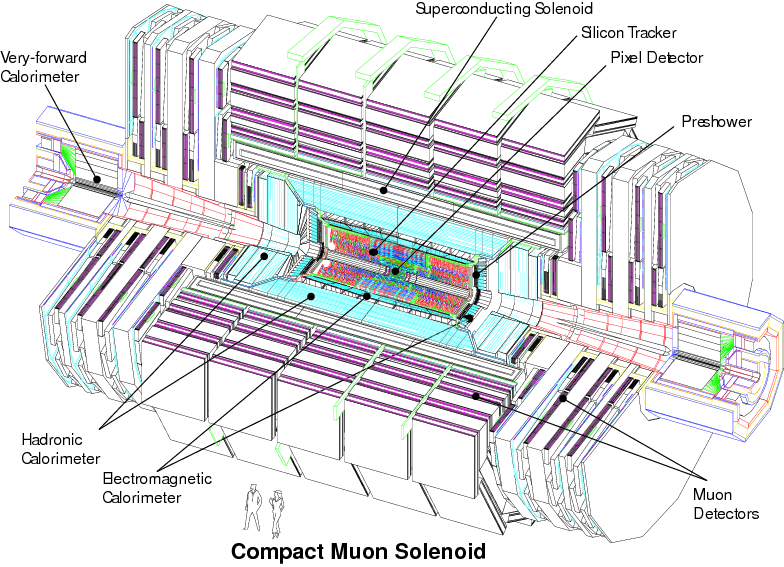
\includegraphics[width=0.65\textwidth]{figures/cms/cms.png}
        \caption{Cut-away view of the CMS detector and its subsystems.
                 Reprinted from Reference~\cite{cmsjinst}.}
        \label{fig:cms:cms}
    \end{center}
\end{figure}

\subsubsection{Silicon tracker}

Starting from the beam pipe, the first of these subsystems is the silicon tracker~\cite{cmstracker}, used to identify charged particles and measure their momenta. 
The tracker consists of silicon detector geometries: pixels (providing 3D position measurement) and strips (2D). 
The arrangement of the pixel and strip layers are shown in Figure~\ref{fig:cms:si}.
A near-uniform 3.8 T magnetic field, produced by a superconducting NbTi solenoid, envelopes the tracker. 
The field lines in the tracker volume are approximately parallel to the beam direction. 

A single silicon pixel has dimensions $285\times100\times150$ $(\mu\mathrm{m})^3$ (in $r\times r\phi\times z$), leading to a position resolution of $\sim10\times30$ $(\mu\mathrm{m})^2$ (in $r\phi\times z$). 
The 66 million pixels are arranged into 7 layers: 3 cylindrical ``barrels'' (at $r=4.4,~7.3,~10.2$ cm) and $2\times2$ ``endcap'' annulli (at $z=\pm34.5,~\pm46.5$ cm). 
Outside the pixel layers are the strip layers, consisting of 9.3 million silicon strips arranged into barrels and endcaps.
The resolution in $r\phi$ varies between $10$ and $50$ $\mu$m, depending on the location and pitch of the given strip.
Certain strip layers contain two layers of strips, rotated through a ``stereo'' angle (100 mrad) with respect to each other.
By matching adjacent hits, the stereo measurement can add a third dimension ($z$ for barrel, $r$ for endcap) to the strip's 2D measurement, with resolution $100$-$500$ $\mu$m.
There are a total of 10 barrel layers ($0.2 < r < 1$ m) and 24 endcap layers ($0.6 < |z| < 2.8$ m). 

\begin{figure}
    \begin{center} 
        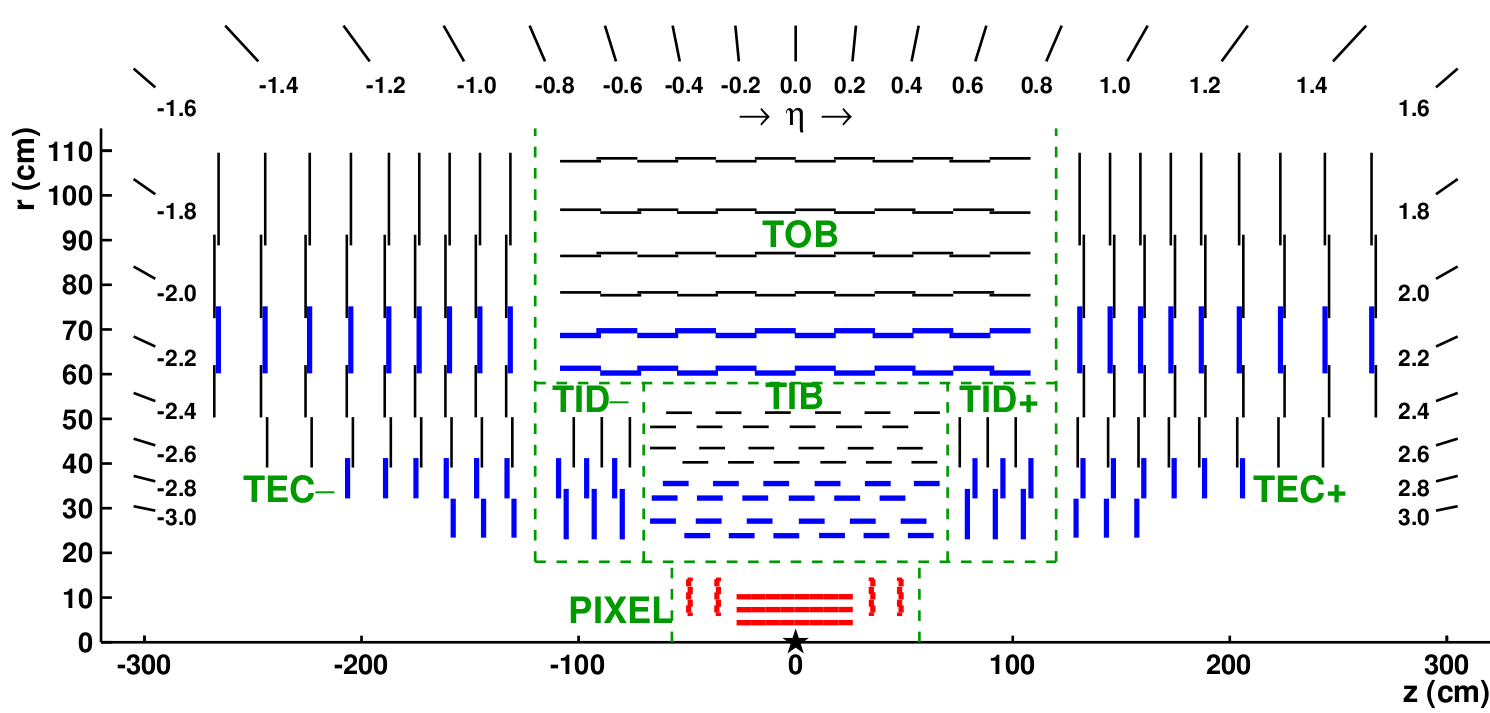
\includegraphics[width=0.7\textwidth]{figures/cms/tracker.png}
        \caption{Diagram of a slice of the CMS tracking system.
                 The pixel layers are shown in bold red lines.
                 Single-strip (double-strip) layers are indicated by thin black (bold blue) lines.
                 The double-strip modules each consist of two back-to-back strips, rotated with respect to each other, that can provide 3D localization of the hits.
                 Reprinted from Reference~\cite{cmstracker}.}
        \label{fig:cms:si}
    \end{center}
\end{figure}

Pixels with a signal greater than a tuneable readout threshold (typically around $3000 Q_e$) are read out.
These pixels are then aggregated with adjacent signals to form pixel clusters, which are further subjected to readout thresholds ($\sim 4000 Q_e$).
The exact position of the particle in this layer (known as a ``hit'') is inferred by fitting the charge distribution of the pixels in this cluster to pre-determined templates.
A similar method is employed to determine the strip hit positions, with some modifications to account for Lorentz drift of the charges in the silicon detector due to the $B$-field. 
The efficiency of reconstructing hits varies with the detector type, location, and particle momentum, but is generally greater than $99\%$ ($99.5\%$ if defective modules are not considered). 

Tracks are found using an iterative ``inside-out'' process, where each iteration has five steps:
\begin{enumerate}
    \item Define seeds using pixel hits, double-strip hits (i.e. hits with 3D information), and an estimate of the beam spot (collision point). At least 3 hits are needed for the seed.
    \item Use a Kalman filter~\needcite to evolve track seeds through the rest of the tracker and find hits, accounting for the $B$-field and energy loss.
    \item Estimate trajectory parameters after finding all hits.
    \item Decide whether to keep found tracks based on quality requirements (e.g. number of missing hits, track $\chi^2$)
    \item Remove hits associated with tracks from hit collection and repeat.
\end{enumerate}
The trajectory parameters referred to in step 3 are the 5 parameters of a helix: $\rho$ (curvature), $\phi_0$ (azimuthal angle), $\lambda$ ($\cot\theta$), $d_0$ (``impact parameter'', minimum $r$ of track), $z_0$ (minimum $|z|$ of track).
The CMS track fit typically has 5-7 iterations, with each successive iteration loosening the seed and track fit requirements to look for more difficult tracks (e.g. missing hits, large $d_0$).
The efficiency and fake rate of this reconstruction, as a function of track \pt, are shown in Figure~\ref{fig:cms:trackeff}.
For muons with $|\eta|<1.5$ and $\pt>1$ GeV, the tracking efficiency is over 98\%, with a combinatorial fake rate of 2-6\%. 

\begin{figure}
    \begin{center} 
        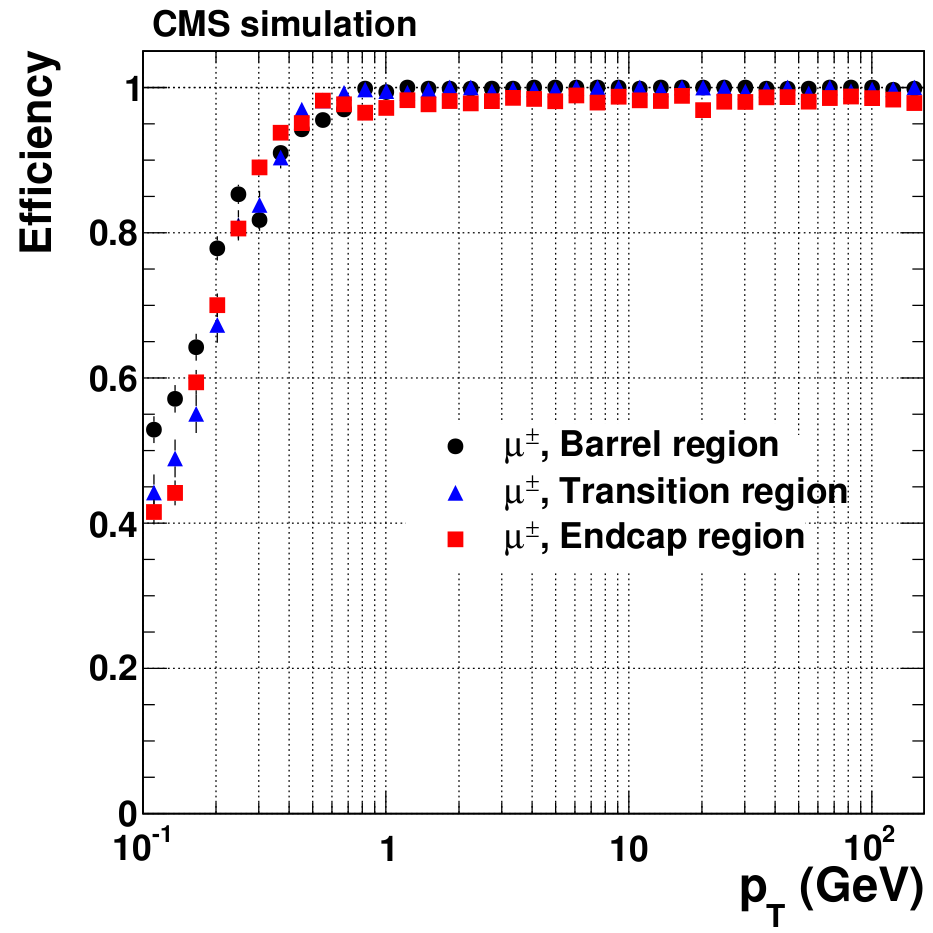
\includegraphics[width=0.35\textwidth]{figures/cms/track_eff.png}
        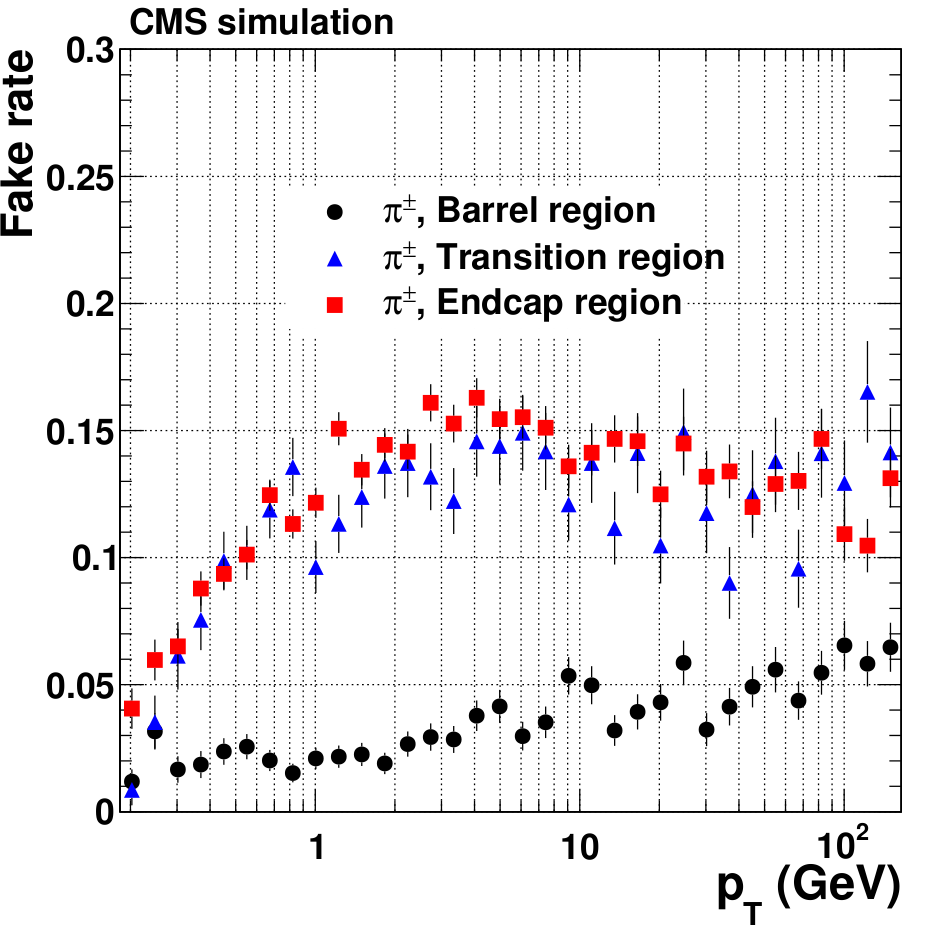
\includegraphics[width=0.35\textwidth]{figures/cms/track_fake.png}
        \caption{Efficiency (fake rate) of the CMS track fit algorithm, evaluated using simulation of muons (charged pions).
                 Reprinted from Reference~\cite{cmstracker}.}
        \label{fig:cms:trackeff}
    \end{center}
\end{figure}

The excellent position resolution of the pixel detector is used to accurately measure the position of primary vertices, as well as any secondary vertices from the decays of long-lived particles.
In the former case, tracks are first clustered together on the basis of the likelihood that the tracks in a cluster arise from a single primary vertex.
This is done using a deterministic annealing algorithm~\cite{da}, which has as free parameters the number of clusters and the probability of each track belonging to each cluster.
Having determined the clusters, an adaptive fit algorithm~\cite{adaptivefit} is used to determine the vertex for each cluster.
The free parameters of this fit are the three spatial coordinates of the vertex.
As the LHC collides bunches of $\mathcal{O}(10^{11})$ protons, we expect multiple primary vertices in a single collision, and this is reflected in Figure~\ref{fig:cms:npv}.
The vertex defined to be the hard scattering interaction (known as \emph{the} primary vertex\footnote{This nomenclature is indeed confusing, defining the singular primary vertex to be one of many primary vertices. However, it is standard terminology in CMS publications, so we will continue to use it. In what follows, the distinction will be clear}) is the vertex which maximizes:
\begin{equation}
	\sum_{j\in\mathrm{track jets}} (\pt^j)^2 + (\ptmiss)^2
\end{equation}
where ``track jets`` refer to jets (Section~\ref{sec:cms:jets}) clustered from the vertex's tracks, and \ptmiss~is defined in Section~\ref{sec:cms:met}.

\begin{figure}
    \begin{center} 
        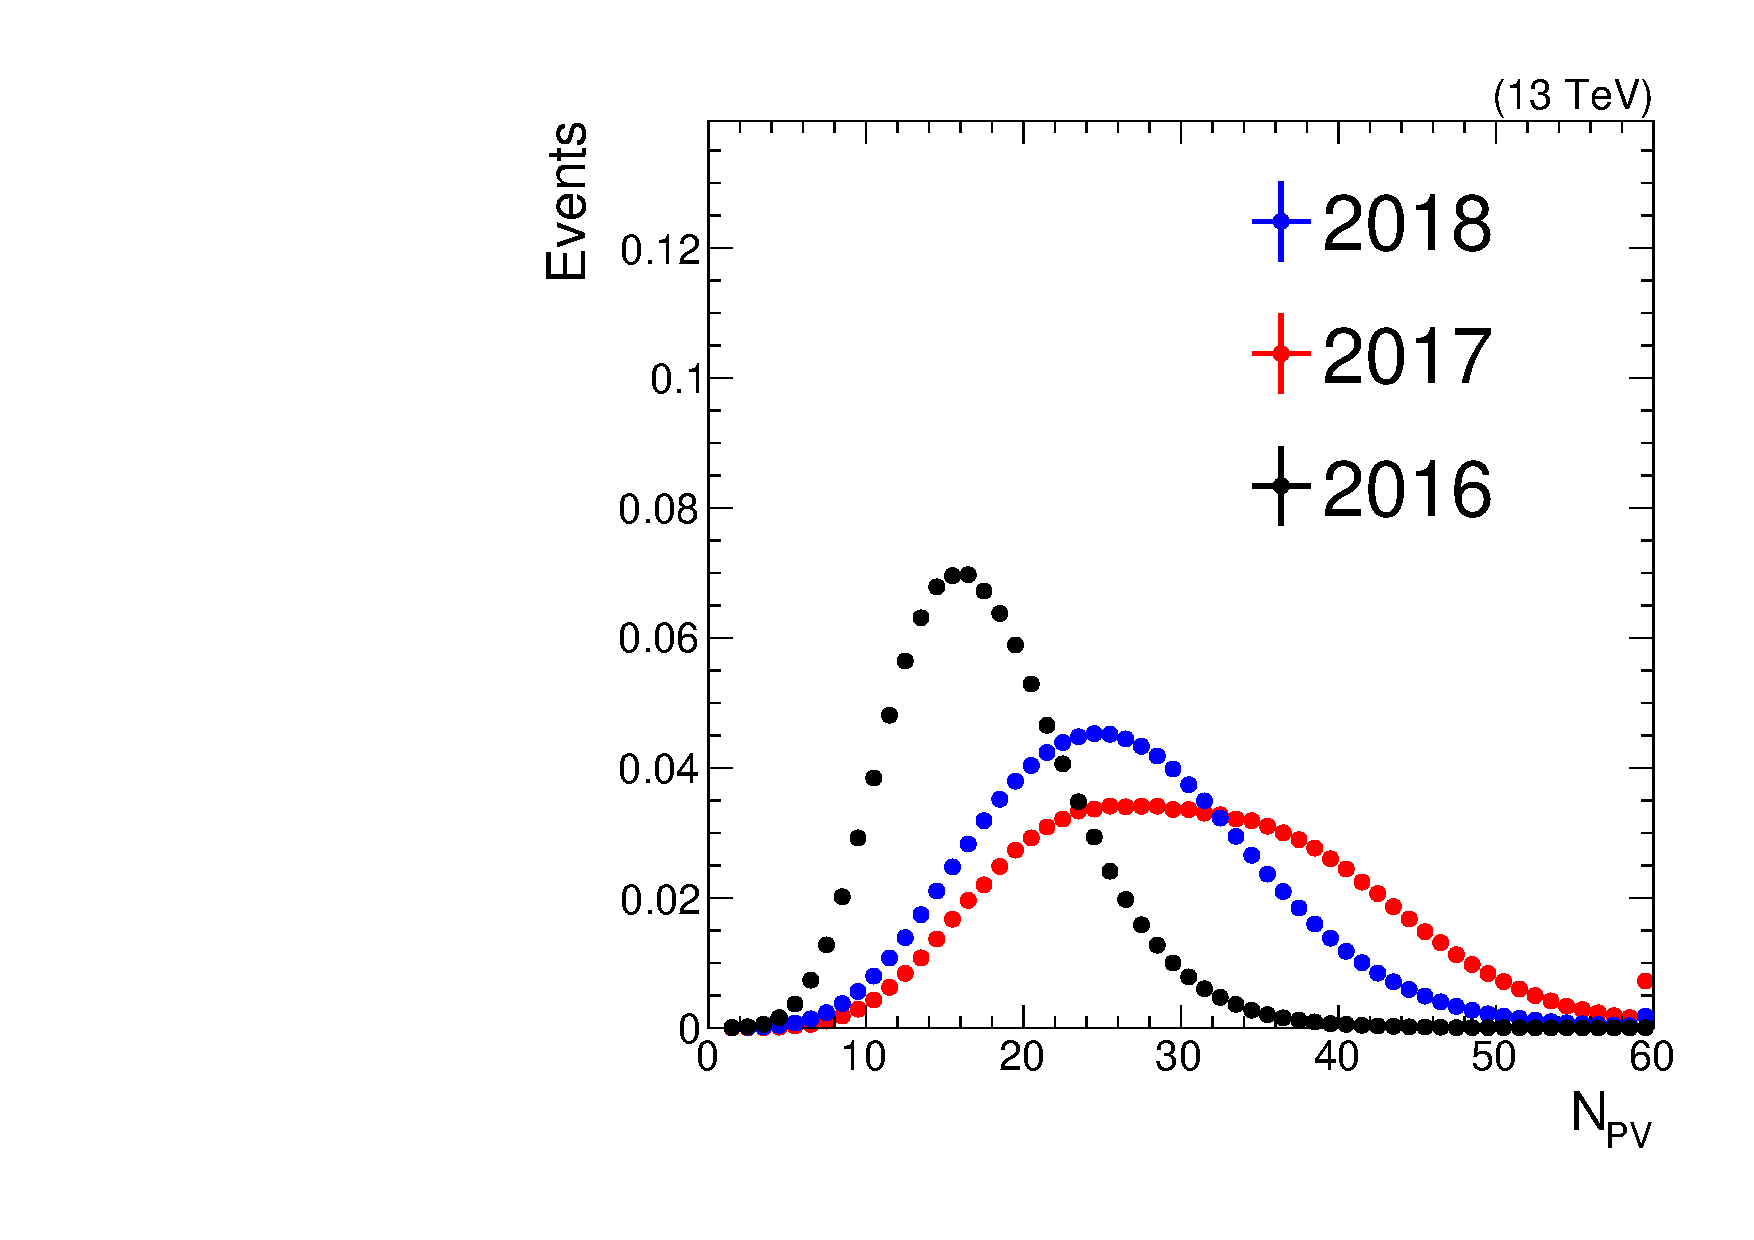
\includegraphics[width=0.7\textwidth]{figures/cms/comparison_npv.pdf}
        \caption{The distribution of the number of reconstructed primary vertices in data recorded by CMS during Run 2 of the LHC.
				 While the results in this thesis only concern 2016 data, we show the evolution of $N_\mathrm{PV}$ as a function of time, as this correlates directly with increased instantaneous luminosity.}
        \label{fig:cms:npv}
    \end{center}
\end{figure}

The last reconstruction algorithm concerning the tracker alone is the identification of secondary vertices, which arise from the decay of long-lived particles (e.g. $B$ mesons).
The inclusive vertex fitter (IVF)~\cite{csvv2} reconstructs such secondary vertices by the following steps:
\begin{enumerate}
	\item Select a track as a seed if it satisfies $\sqrt{d_0^2 + d_z^2} > 50~\mu\mathrm{m}$ and $d_0 > 1.2 \delta d_0$.
	\item Choose nearby tracks based on their closest distance to and opening angle with the seed track.
	\item Fit the tracks to a displaced vertex using the adaptive fitter~\cite{adaptivefit}.
	\item Decide which tracks belong to the candidate secondary vertex and which belong to the primary vertex.
	\item Re-fit the secondary vertex position only using the former set of tracks from the previous step.
\end{enumerate}
It is important not only to properly determine the location of the secondary vertex, but also to properly assign tracks.
Observables that are a function of the \emph{tracks} (e.g. vertex mass) will be critical for $b$ jet tagging.

\subsubsection{Electromagnetic calorimeter}

The CMS electromagnetic calorimeter~\cite{cmsecaljinst} (ECAL) is a homogenous detector with good energy and angular resolution, composed of 76,000 \pbwo~crystals. 
The crystals are arranged in two sections: a cylindrical barrel (EB) covering $|\eta|<1.44$ and two endcap annuli (EE) extending to $|\eta|<3$.
This provides slightly more coverage than the tracking volume.
Each crystal in the EB (EE) has dimensions $2.2\times2.2\times23$ ($2.68\times2.68\times22$) $(\mathrm{cm}^3)$, with the long dimension pointing towards the beam.
This can be compared to a Moli\'ere radius $r_M=2.19$ cm and a radiation length of $X_0=0.89$ cm. 
A cross-sectional area comparable to $r_M\times r_M$ facilitates the differentiation of different electromagnetic (EM) showers arising from electrons and photons.
The depth of the crystal (in units of $X_0$) drives the excellent energy resolution, which is determined using a electron beam:
\begin{equation}
    \frac{\sigma_E}{E} = \frac{2.8\%}{\sqrt{E/\mathrm{GeV}}} \oplus \frac{12\%}{E/\mathrm{GeV}} \oplus 0.3\%
\end{equation}
Scintillation photons from the \pbwo~crystals are collected by avalanche photodiodes (APDs) in the EB and vacuum phototriodes (VPTs) in the EE, which provide amplification factors of 50 and 10, respectively. 

At high momenta, the two photons from a $\pi^0$ decay may merge into a single ECAL crystal. 
This primarily occurs at high $|\eta|$ due to the $z$-boost of the intitial state.
To differentiate one- and two-photon deposits, a ``preshower'' detector sits in front of the EE ($1.6 < |\eta|<2.5$).
The preshower detector consists of a lead absorber and silicon strips.
A photon (or photon pair) initiates a shower in the lead.
The shower can be resolved in the silicon strips, which have resolution $\mathcal{O}(1\mathrm{-}10)$ mm.

The physical placement of all three ECAL components is shown in Figure~\ref{fig:cms:ecal}.

\begin{figure}
    \begin{center} 
        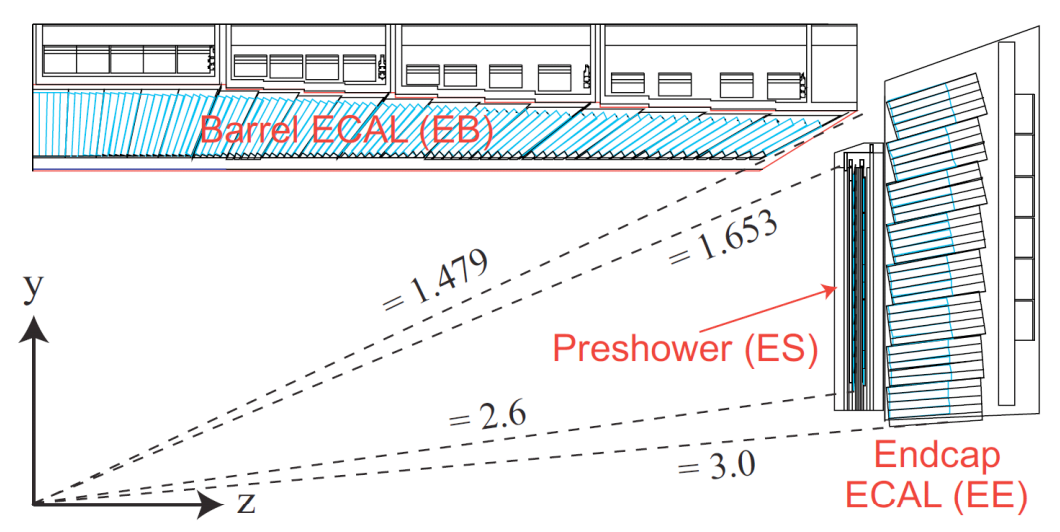
\includegraphics[width=0.7\textwidth]{figures/cms/ecal.png}
        \caption{One quadrant of the CMS ECAL (symmetric with rotation around $z$ and reflection across $z=0$).
                 The dashed lines indicate values of $\eta$.
                 Reprinted from Reference~\cite{cmsecaljinst}.}
        \label{fig:cms:ecal}
    \end{center}
\end{figure}

Due to the bending of a charged particle's trajectory in the solenoidal $B$-field, bremsstrahlung photons will be emitted at similar values of $\eta$, but spread along $\phi$.
A ``supercluster'' (SC) is defined by clustering nearby ECAL energy depositions, allowing for a wider spread in $\phi$ than in $\eta$ (Figure~\ref{fig:cms:sc}).
The particle's EM energy is defined to be the weighted sum of the energies of all crystals in the SC, where the coefficients account for crystal-specific calibration effects.
For an electron or photon, the EM energy is typically the energy of the particle, whereas for other particles (charged hadrons and some muons), it is only a fraction of the total energy.

\begin{figure}
    \begin{center} 
        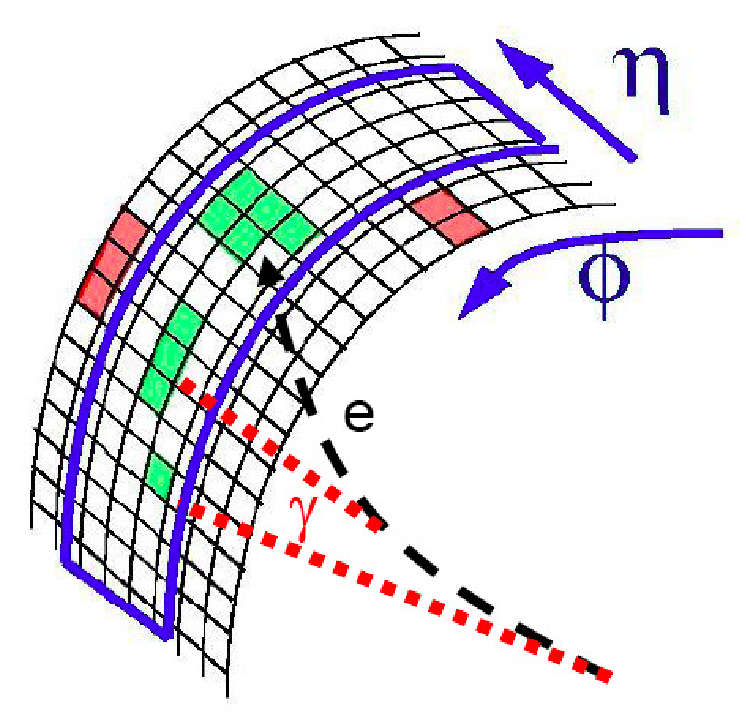
\includegraphics[width=0.3\textwidth]{figures/cms/sc.png}
        \caption{The combination of multiple ECAL crystals into a single supercluster, intended to capture energy depositions from bremsstrahlung photons.
                  Reprinted from Reference~\cite{cmsecalrev}.}
        \label{fig:cms:sc}
    \end{center}
\end{figure}

\subsubsection{Hadronic calorimeter}

\subsubsection{Muon chambers}

\subsubsection{Online trigger system}

\section{Particle reconstruction and identification}

\subsubsection{Particle flow algorithm}

Because of the excellent angular granularity of the CMS detector and the momentum resolution of the tracker, a particle flow~\cite{cmspf} algorithm is used to correlate information from all detector subsystems to build a global description of each event.
Particle flow (PF) algorithms date back to ALEPH~\needcite, and are in contrast to detector-specific physics object-based algorithms used at other experiments (e.g. References~\needcite).

The key feature of the PF algorithm is to ``link'' multiple detector signals together into a single PF candidate.
This linkage combines inner tracks, ECAL clusters, HCAL clusters, and muon tracks based on their proximity in the $(\eta,\phi)$ plane.
Inner track helices are extended into the calorimeters, searching for clusters compatible with the trajectory.
Similarly, clusters from the ECAL, the ECAL preshower, and the HCAL can be linked without a track present. 


\subsubsection{Electrons and photons}

Both electrons and photons are seeded using ECAL SCs.


\subsubsection{Jets}
\label{sec:cms:jets}

\subsubsection{Muons}

\subsubsection{Hadronic taus}

\subsubsection{Missing momentum}
\label{sec:cms:met}


\section{Simulation of collisions}

\subsection{Physics simulation}

\subsection{Detector simulation}

\chapter{Hadronic Resonance Identification}
\label{sec:jets}

In this chapter, we describe the reconstruction and identification of heavy ($\gtrsim 100$ GeV) resonances that decay to two or more quarks.
Within the Standard Model, the only such resonances are the massive vector bosons ($W,Z\rightarrow q\bar{q}'$), the Higgs boson (typically $H\rightarrow b\bar{b}$), and the top quark ($t\rightarrow bW(\rightarrow q\bar{q}')$).
These quarks hadronize into jets (described in Chapter~\ref{sec:theory}), which are typically reconstructed at the LHC using the anti-$k_\mathrm{T}$ algorithm (described in Chapter~\ref{sec:cms}).
The focus of this chapter is on the cases in which the resonance is boosted and the decay products merge, such that they cannot be identified as 2 or 3 distinct jets.
In preparation for Chapter~\ref{sec:mt}, we will take the top quark as a concrete example.
The studies presented here can (and in some cases have been) applied to other heavy resonances, both within and beyond the Standard Model.

\section{Reconstruction}
\label{sec:jets:reco}

The approximate angular separation between the quarks from a heavy resonance decay is\needcite:
\begin{equation}
    \Delta R \sim \frac{2M}{\pt}
\end{equation}
where $M$ is the resonance mass and $\pt$ is the resonance transverse momentum.
Setting $M=m_t$ and $\Delta R=1.2$ (i.e.~the radius at which three $R=0.4$ jets start to overlap), we extract a ``merging scale'' of $300$ GeV.  
This is be verified by checking the distribution of the ``decay radius'' in top quark simulation.
Here, we define decay radius as: 
\begin{equation}
    \max\Delta R_{qq} \equiv \displaystyle\max_{0\leq i < j \leq 2} \{\Delta R(q_i,q_j)\} \text{, where } t\rightarrow q_0q_1q_2
\end{equation}
Using a broad spectrum of generated top quark $\pt$, Figure~\ref{fig:jets:dr} shows the dependence of the decay radius on the top quark $\pt$, where we restrict the resonance to satisfy $|\eta|<2.5$.
If we are interested in top quarks with $\pt>250$ GeV (motivated by the trigger selection (Section~\ref{sec:mt:sel})), then over half of top quarks will be fully contained within a jet of radius $1.5$.
That is, at $\pt\approx 250$ GeV, it is equally likely that a top quark's decay products will fall within a single large-radius jet or that they will be resolvable as three separate jets. 
However, past this threshold momentum, the large-radius jet becomes the preferred reconstruction option.
This motivates the use of $R=1.5$ jets to reconstruct hadronic top quarks with $\pt>250$ GeV. 

\begin{figure}[]
    \begin{center}
        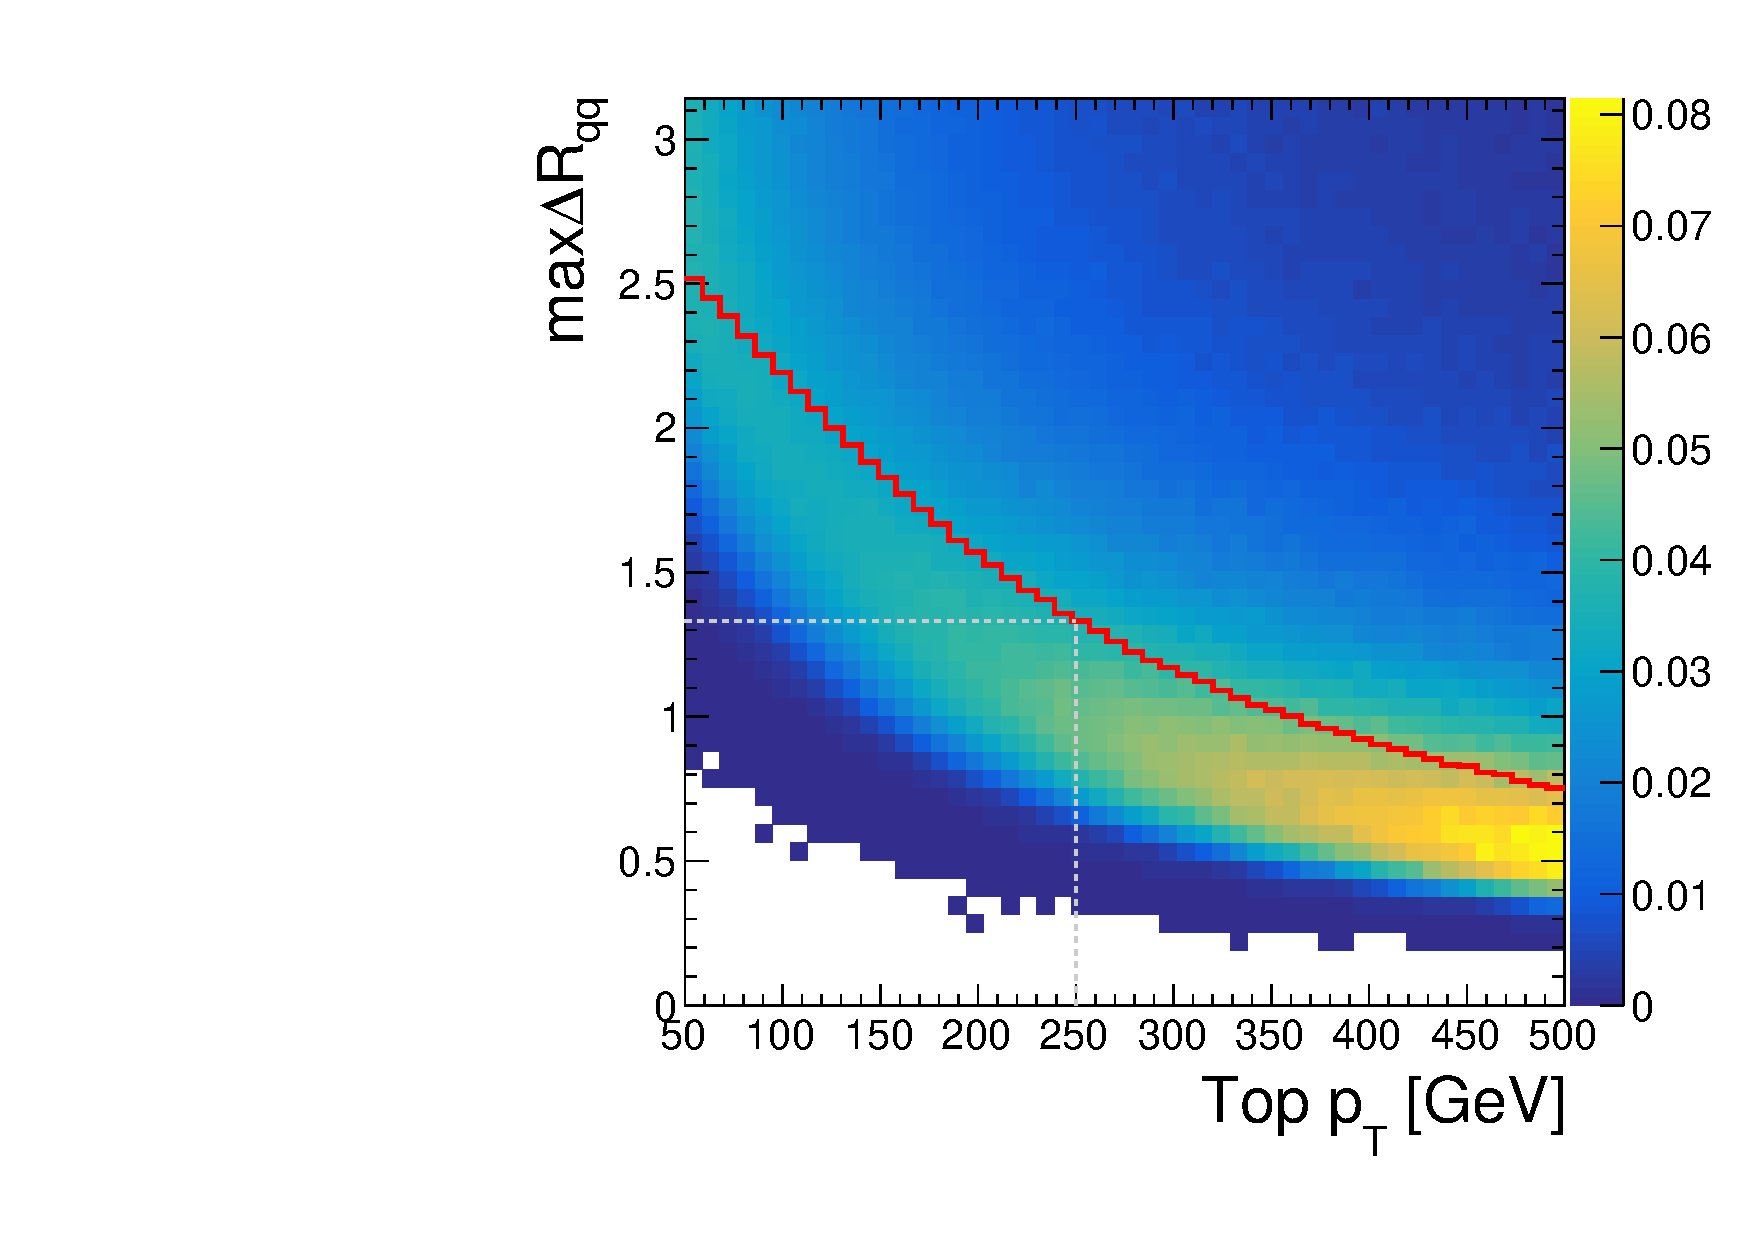
\includegraphics[width=0.5\textwidth]{figures/toptagging/gen/ptdr.pdf}
        \caption{Distribution of top quark momenta versus decay radii in a simulated top quark pair sample.
                 The events are weighted such that the inclusive momentum distribution is uniform. 
                 The $z$-axis units are arbitrary, but proportional to the distribution of jets. 
                 The solid red line marks the 50\% quantile of jets at each value of $\pt$. }
        \label{fig:jets:dr}
    \end{center}
\end{figure}

There are two tunable parameters in jet reconstruction.
We have specified the jet radius, but we must also choose the jet algorithm.
The anti-$k_\mathrm{T}$ algorithm tends to pick circular jets, whereas the Cambridge-Aachen (CA) algorithm allows for more geometric shapes (Figure~\ref{fig:jets:algos}).
As the top jets we seek to reconstruct are the sum of three light quark jets, we do not necessarily expect the $R=1.5$ jet to be circular.
Figure~\ref{fig:jets:caak} compares the jet mass distribution for top and light quark/gluon (LQG) jets, where the jets are clustered using both algorithms.
CA produces a top jet mass distribution with a narrower peak that sits closer to $m_t$ than anti-\kt. 
Because of this, and the general improvement in $S/B$ near the top mass peak, we choose the CA algorithm.
Hereafter, we will refer to Cambridge-Aachen $R=1.5$ jets as CA15 jets. 

\begin{figure}[]
    \begin{center}
        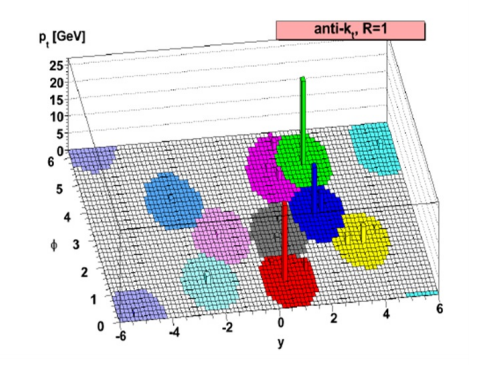
\includegraphics[width=0.35\textwidth]{figures/toptagging/gen/ak.png}
        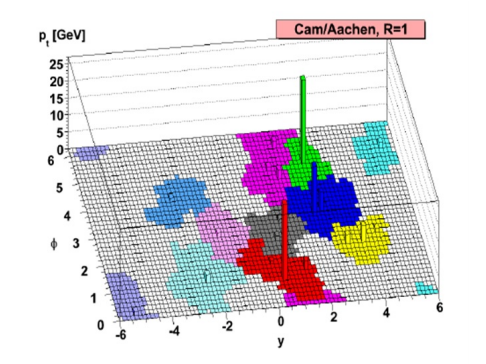
\includegraphics[width=0.35\textwidth]{figures/toptagging/gen/ca.png}
        \caption{Jets clustered using the anti-$k_\mathrm{T}$ (left) and CA (right) algorithms.
                 Shown is the $y$-$\phi$ plane of a hypothetical calorimeter, unrolled onto a flat surface.
                 The height of each cell represents the \pt~of the particle. 
                 The anti-\kt~jets tend to be more circular when compared to the CA jets.
                 Figures are adapted from~\needcite.}
        \label{fig:jets:algos}
    \end{center}
\end{figure}

\begin{figure}[]
    \begin{center}
        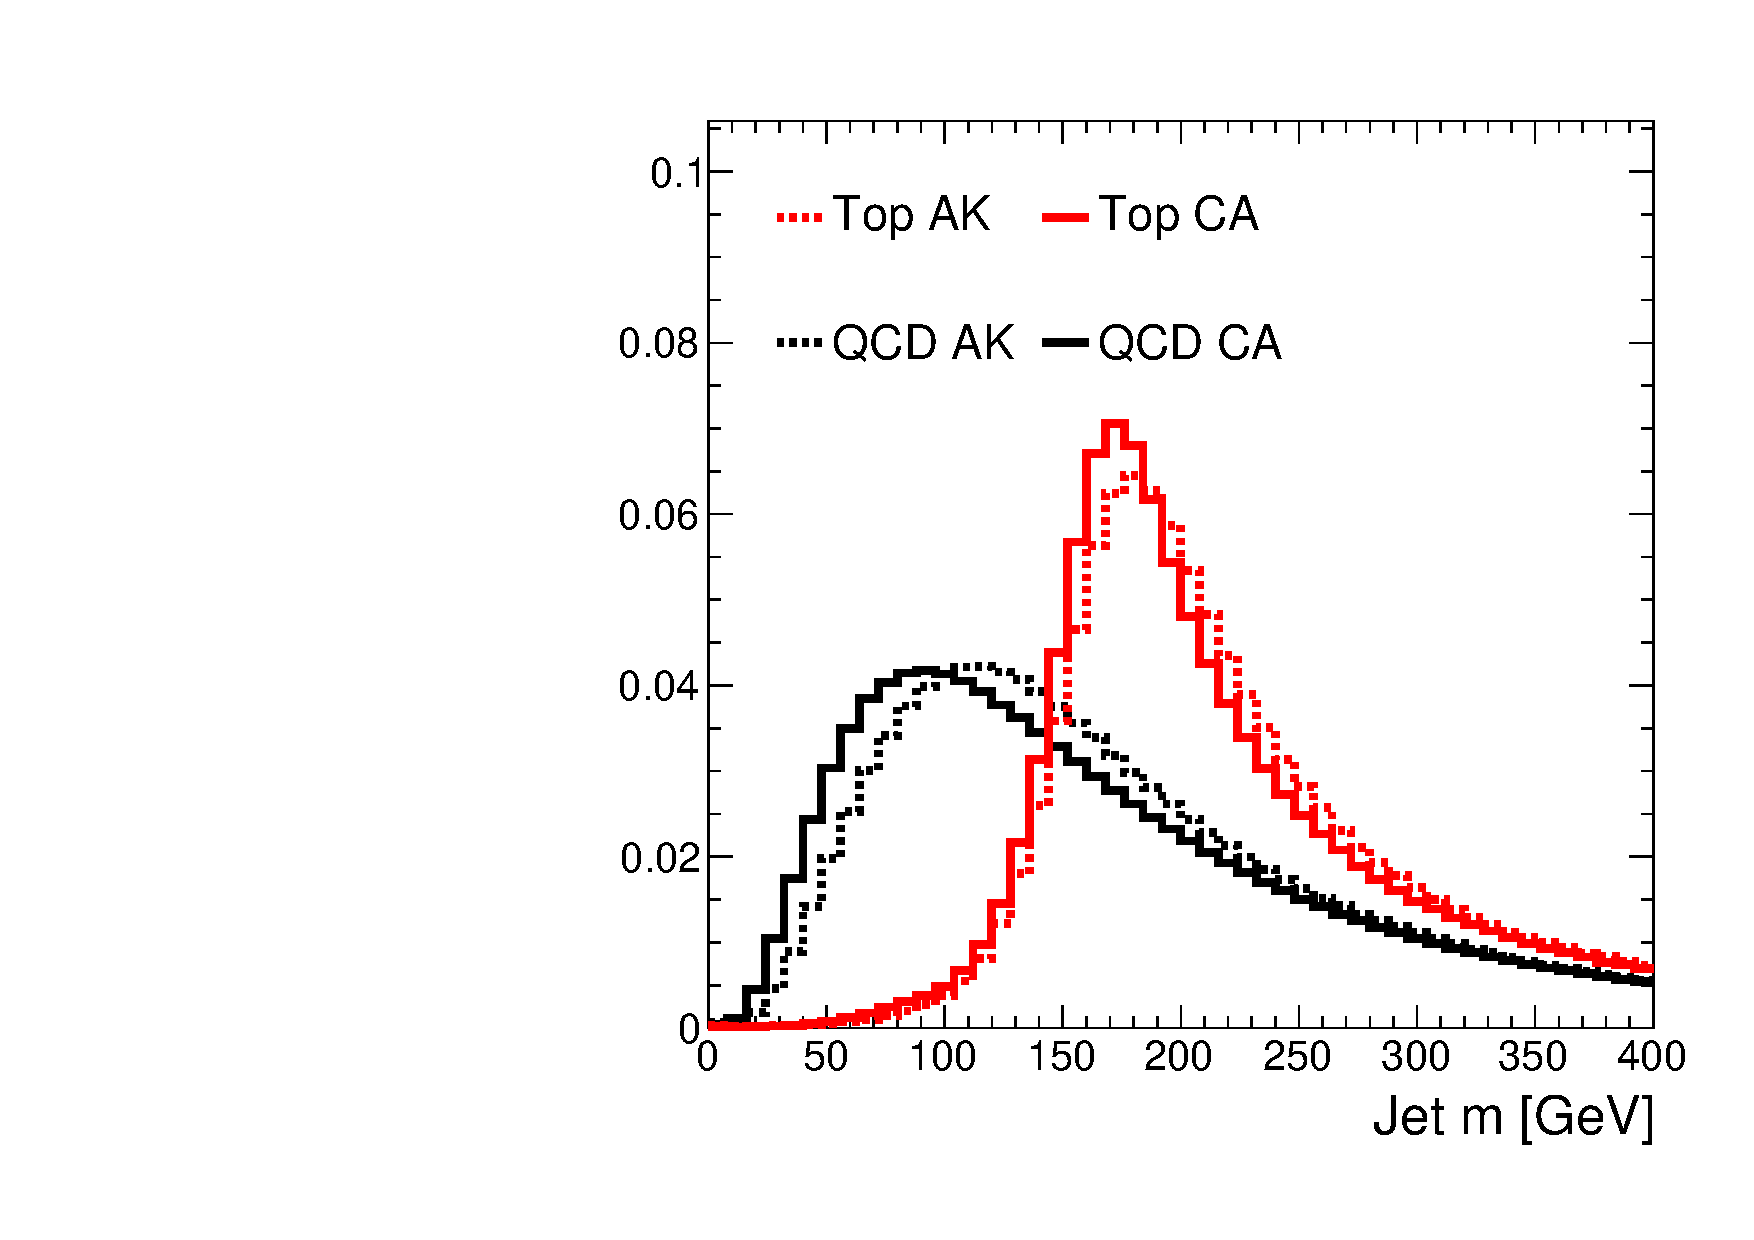
\includegraphics[width=0.5\textwidth]{figures/toptagging/gen/clf_M.pdf}
        \caption{Mass distribution for jets clustered using the anti-$k_\mathrm{T}$ (dashed) and CA (solid) algorithms.
                 QCD refers to jets originating in QCD multijet events, i.e.~from the hadronization of light quarks or gluons.}
        \label{fig:jets:caak}
    \end{center}
\end{figure}

The distance parameter of $R=1.5$ corresponds approximately to a maximal azimuthal angle separation of $\nicefrac{\pi}{2}$, which can cover half of the detector's fiducial volume.
As the jet is so large, particles from pile-up interactions may accidentally be clustered into a jet from the primary vertex.
Fundamental quantities (like top quark momentum) are uncorrelated with the number of primary vertices (\NPV), but reconstructed quantities acquire such a dependence due to the extra radiation.
These additional particles bias the energy scale of the jet (e.g. the mass) as well as geometric observables (described in Section~\ref{sec:jets:id}).
To mitigate these effects, we scale the particles' 4-momenta by their corresponding PUPPI scores (described in Chapter~\ref{sec:cms}) prior to clustering the jet.
Jets clustered using all particles (without PUPPI filtering) have a jet mass and $\tau_{32}^\mathrm{SD}$ distributions (Figure~\ref{fig:jets:puppi}) in which both the mean and variance have an \NPV-dependence.
Adding PUPPI stabilizes the mean and ensures that the variance does not grow at large \NPV.

\begin{figure}[]
    \begin{center}
        \begin{subfigure}[t]{0.35\textwidth}
            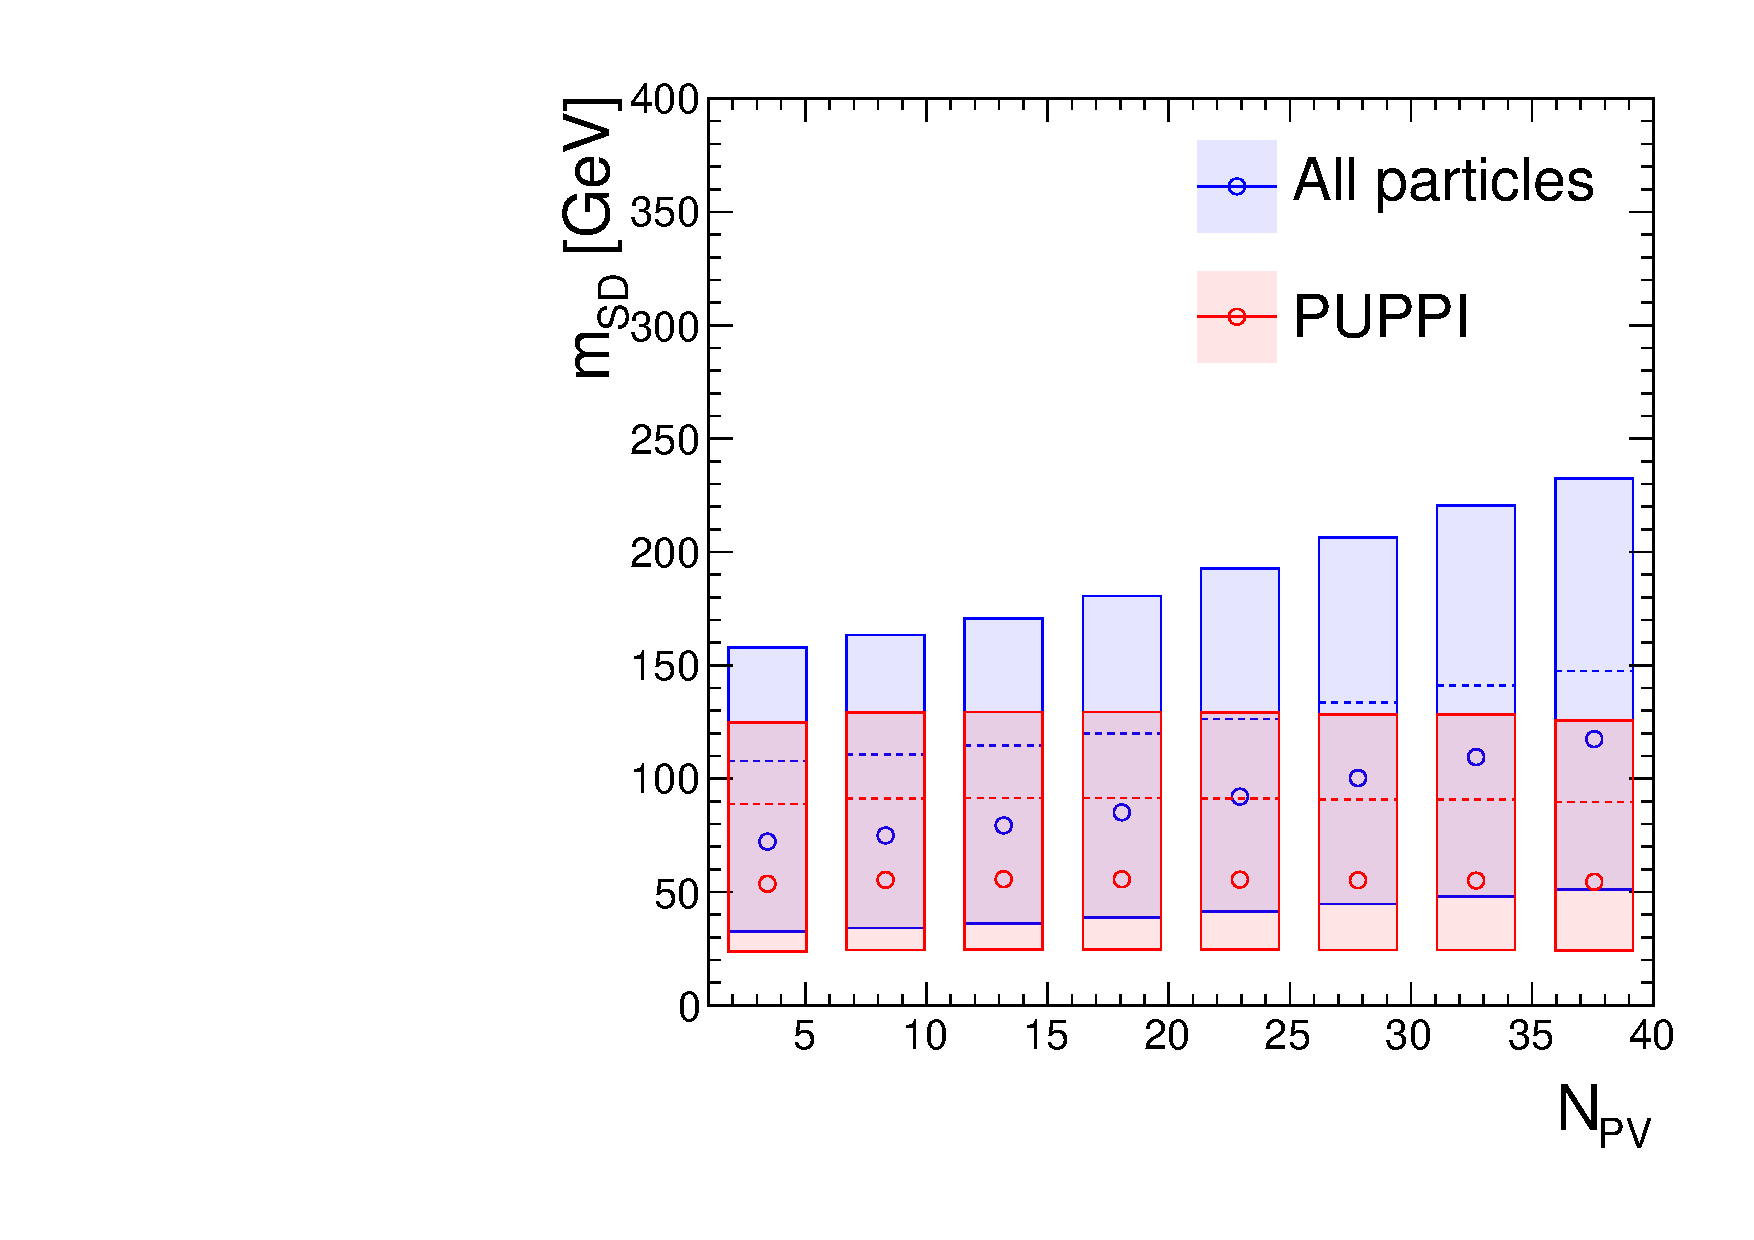
\includegraphics[width=\textwidth]{figures/toptagging/gen/npv_clf_MSD_QCD.pdf}
            \caption{Jet mass, LQG}
        \end{subfigure}
        \begin{subfigure}[t]{0.35\textwidth}
            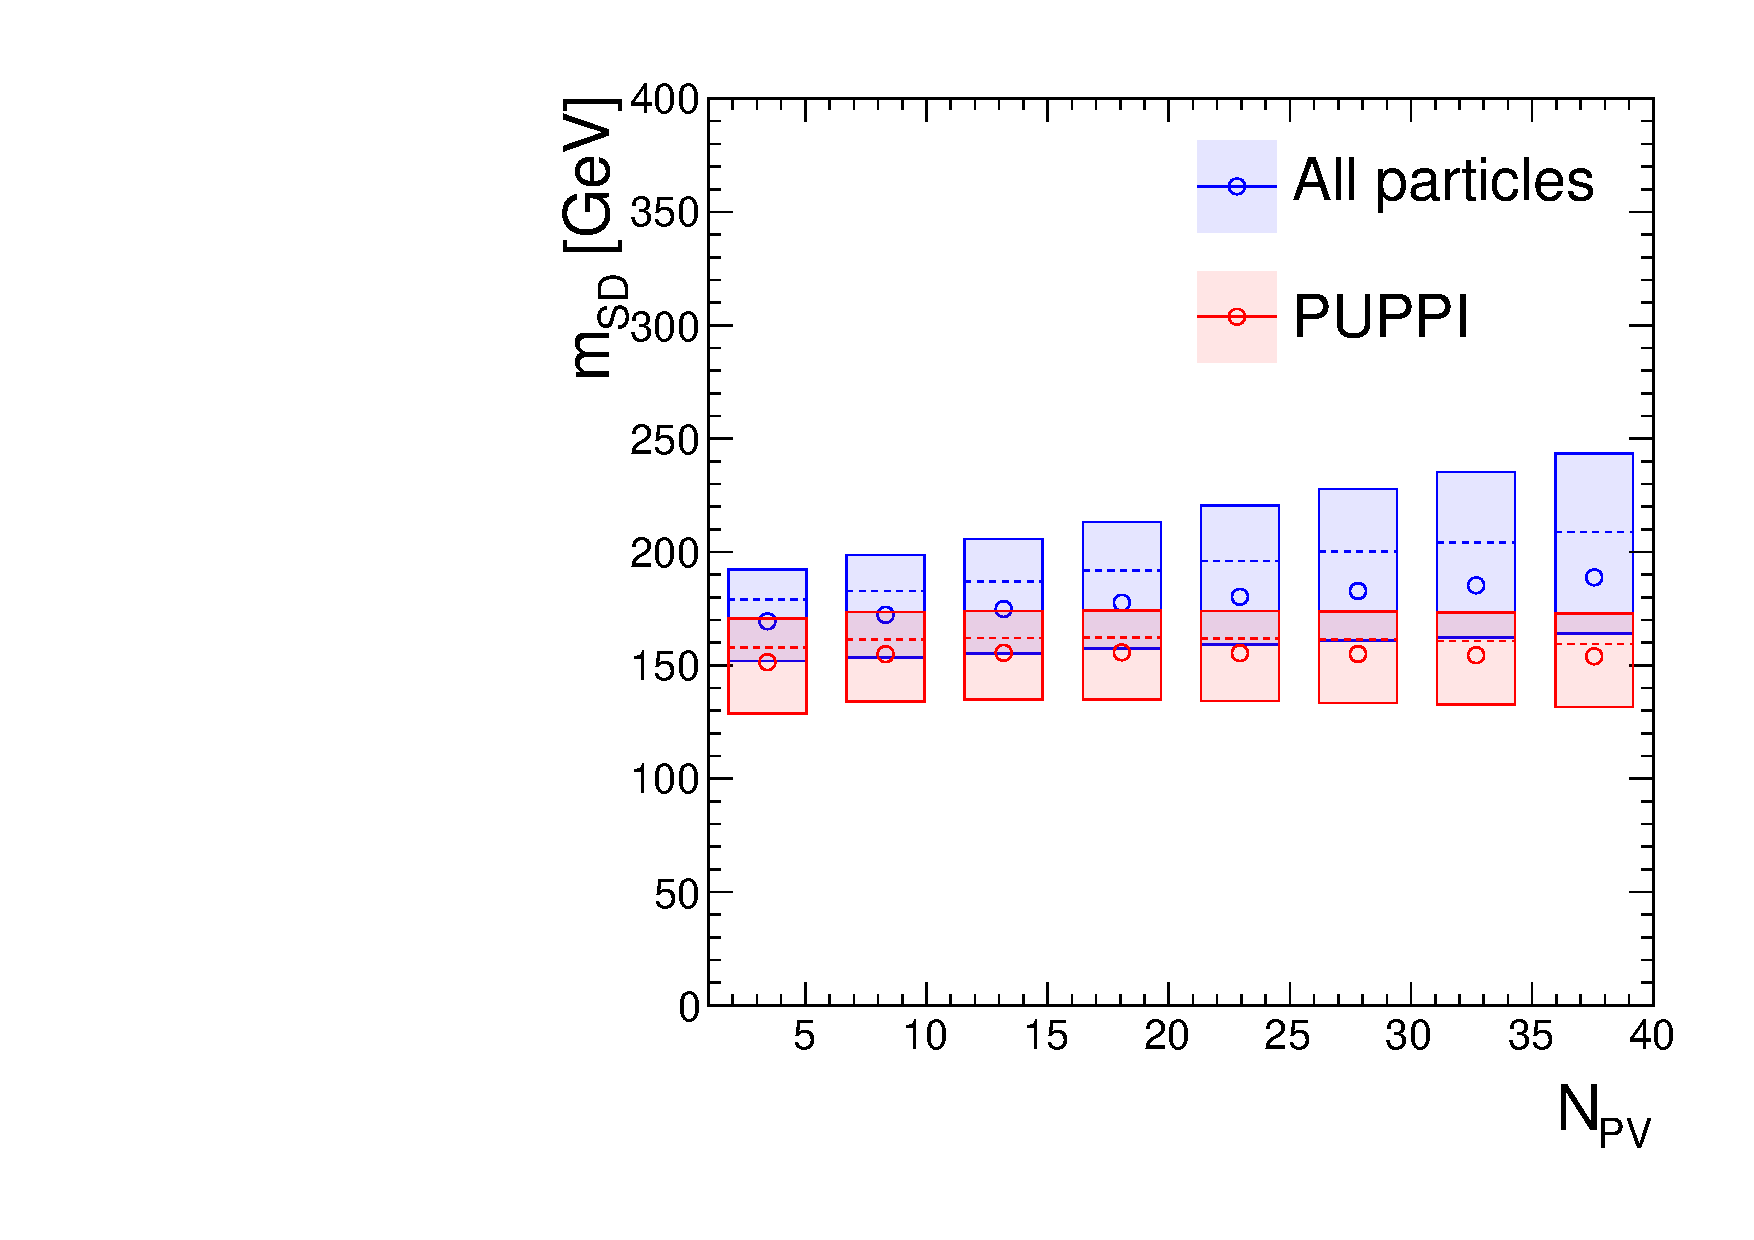
\includegraphics[width=\textwidth]{figures/toptagging/gen/npv_clf_MSD_ZpTT_lo.pdf}
            \caption{Jet mass, Top}
        \end{subfigure}
        \begin{subfigure}[t]{0.35\textwidth}
            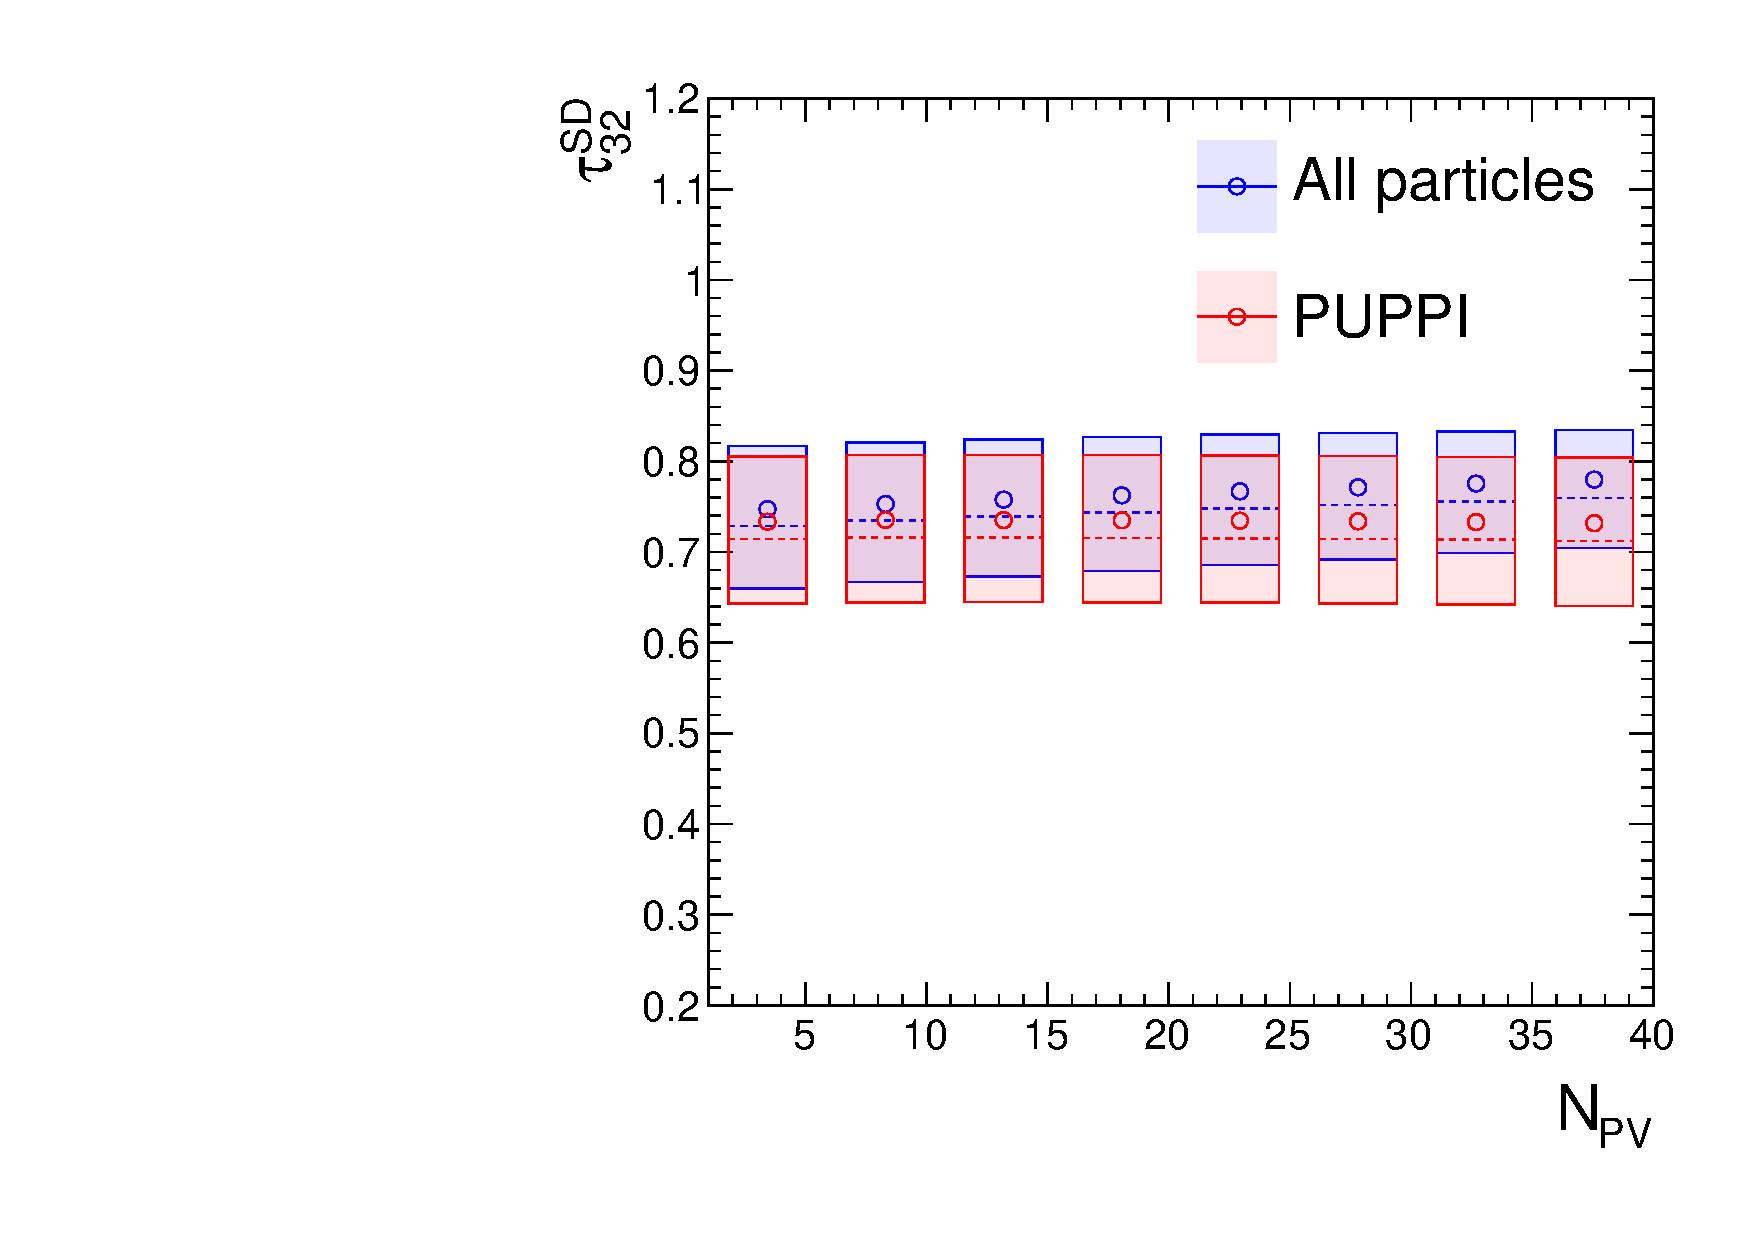
\includegraphics[width=\textwidth]{figures/toptagging/gen/npv_clf_Tau32SD_QCD.pdf}
            \caption{$\tau_{32}^\SD$, LQG}
        \end{subfigure}
        \begin{subfigure}[t]{0.35\textwidth}
            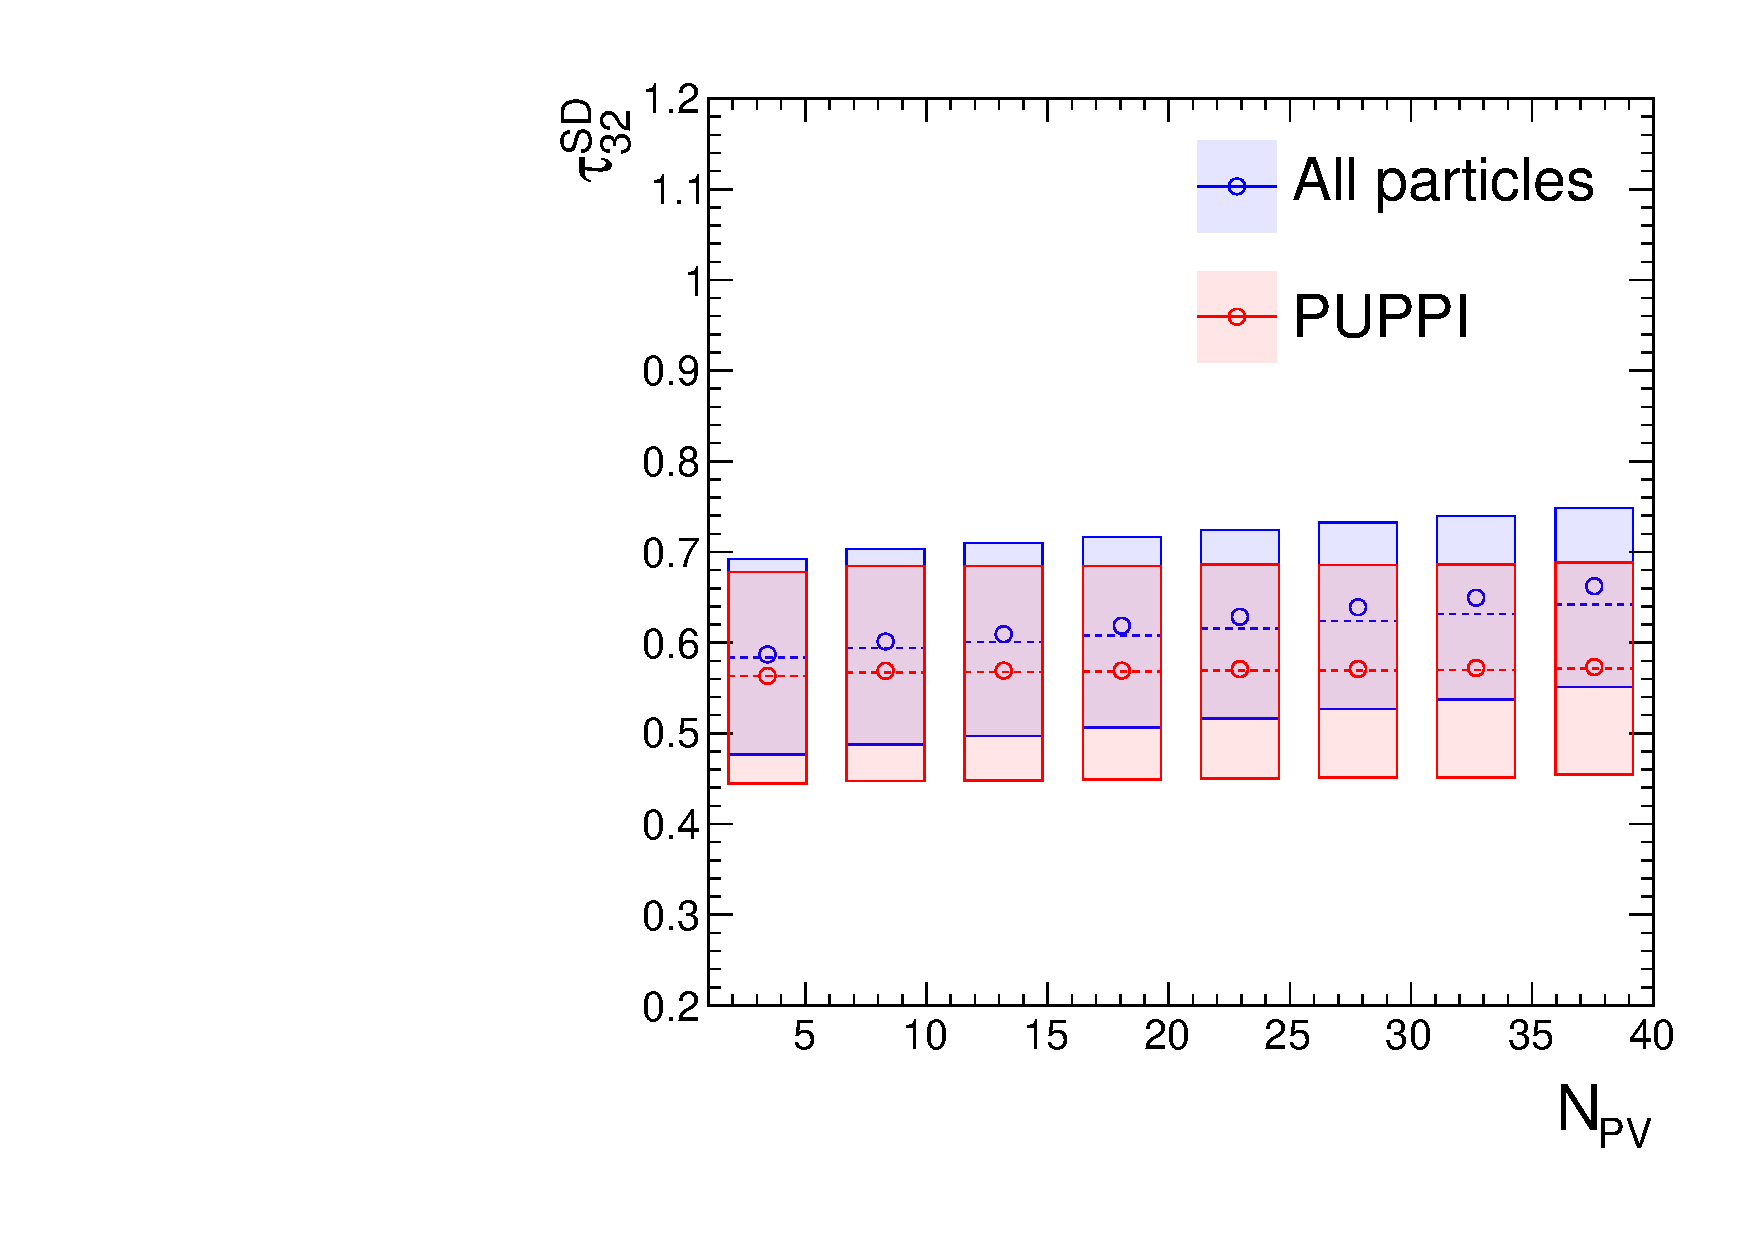
\includegraphics[width=\textwidth]{figures/toptagging/gen/npv_clf_Tau32SD_ZpTT_lo.pdf}
            \caption{$\tau_{32}^\SD$, Top}
        \end{subfigure}
        \caption{Stability of two CA15 jet observables (described in Section~\ref{sec:jets:id}) as a function of $N_\mathrm{PV}$.
            The median (mean) of each \NPV~bin is represented by an open circle (dashed line), while the $[25\%,75\%]$ percentile range is shown with a box.}
        \label{fig:jets:puppi}
    \end{center}
\end{figure}


\section{Identification}
\label{sec:jets:id}

Having \emph{reconstructed} the candidate top quark jets, we turn to the problem of \emph{identifying} which CA15 jets originate from top quarks as opposed to light $q/g$ hadronization. 
As indicated in Figure~\ref{fig:jets:caak}, the jet mass is a powerful observable, but top (LQG) jets do not necessarily have a mass of $m_t$ ($m_q,m_g\sim 0$). 
While some of this discrepancy is caused by mismeasurement of the jet energy scale (Chapter~\ref{sec:cms}), a substantial fraction originates from extra radiation being absorbed into the jet.
These extra particles arise from pile-up (although this is accounted for by PUPPI), initial state radiation, and underlying event.
Many algorithms exist to ``groom'' such particles from a jet after it has been clustered; here, we will discuss and use the soft drop (SD) method~\needcite.
SD functions by traversing the CA clustering history (a binary tree) in reverse and removing subjets (i.e.~branches) of the clustering tree that are deemed to be too soft or wide-angled.
More formally, at each node in the clustering tree, the softer subjet of the node will be removed if it satisfies the condition:
\begin{equation}
    \frac{\min(p_\mathrm{T,1},p_\mathrm{T,2})}{p_\mathrm{T,1}+p_\mathrm{T,2}} < 
    \left(\frac{\Delta R_{12}}{R}\right)^\beta
\end{equation}
where $p_\mathrm{T,i}$ refers to the \pt~of the $i$-th subjet of the node; $\Delta R_{12}$ is the $\Delta R$-distance between the two subjet; and $R$ and $\beta$ are tunable parameters. 
This process starts at the root node of the clustering tree (i.e.~the whole jet) and proceeds iteratively to the leaves (i.e.~individual particles).
This condition is satisfied if the two subjets are very far apart (assuming $\beta \geq 0)$ or if the splitting is very asymmetric in momentum. 
We define the ``SD subjets'' (or where clear, simply ``subjets'') of a jet to be the two branches of the root node, after branches failing the SD condition have been removed. 
The particles remaining after this grooming procedure are combined to make the ``groomed'' or SD jet. 

We then define $m_\mathrm{SD}$ as the mass of the SD jet. 
Observables may also be defined in terms of the groomed or ungroomed jet. 
Figure~\ref{fig:jets:msd} compares the ungroomed and groomed mass distributions in top and LQG jets, as a function of jet momentum. 
It is immediately clear that grooming provides (a) a sharper mass peak in top jets at $m_t$ and (b) a smoothly falling mass distribution in LQG jets that goes to 0.
Furthermore, SD ensures the stability of the mass distribution as a function of jet \pt, especially in LQG jets.
For these reasons, $m_\mathrm{SD}$ will be our standard definition of jet mass. 


\begin{figure}[]
    \begin{center}
        \begin{subfigure}[t]{0.35\textwidth}
            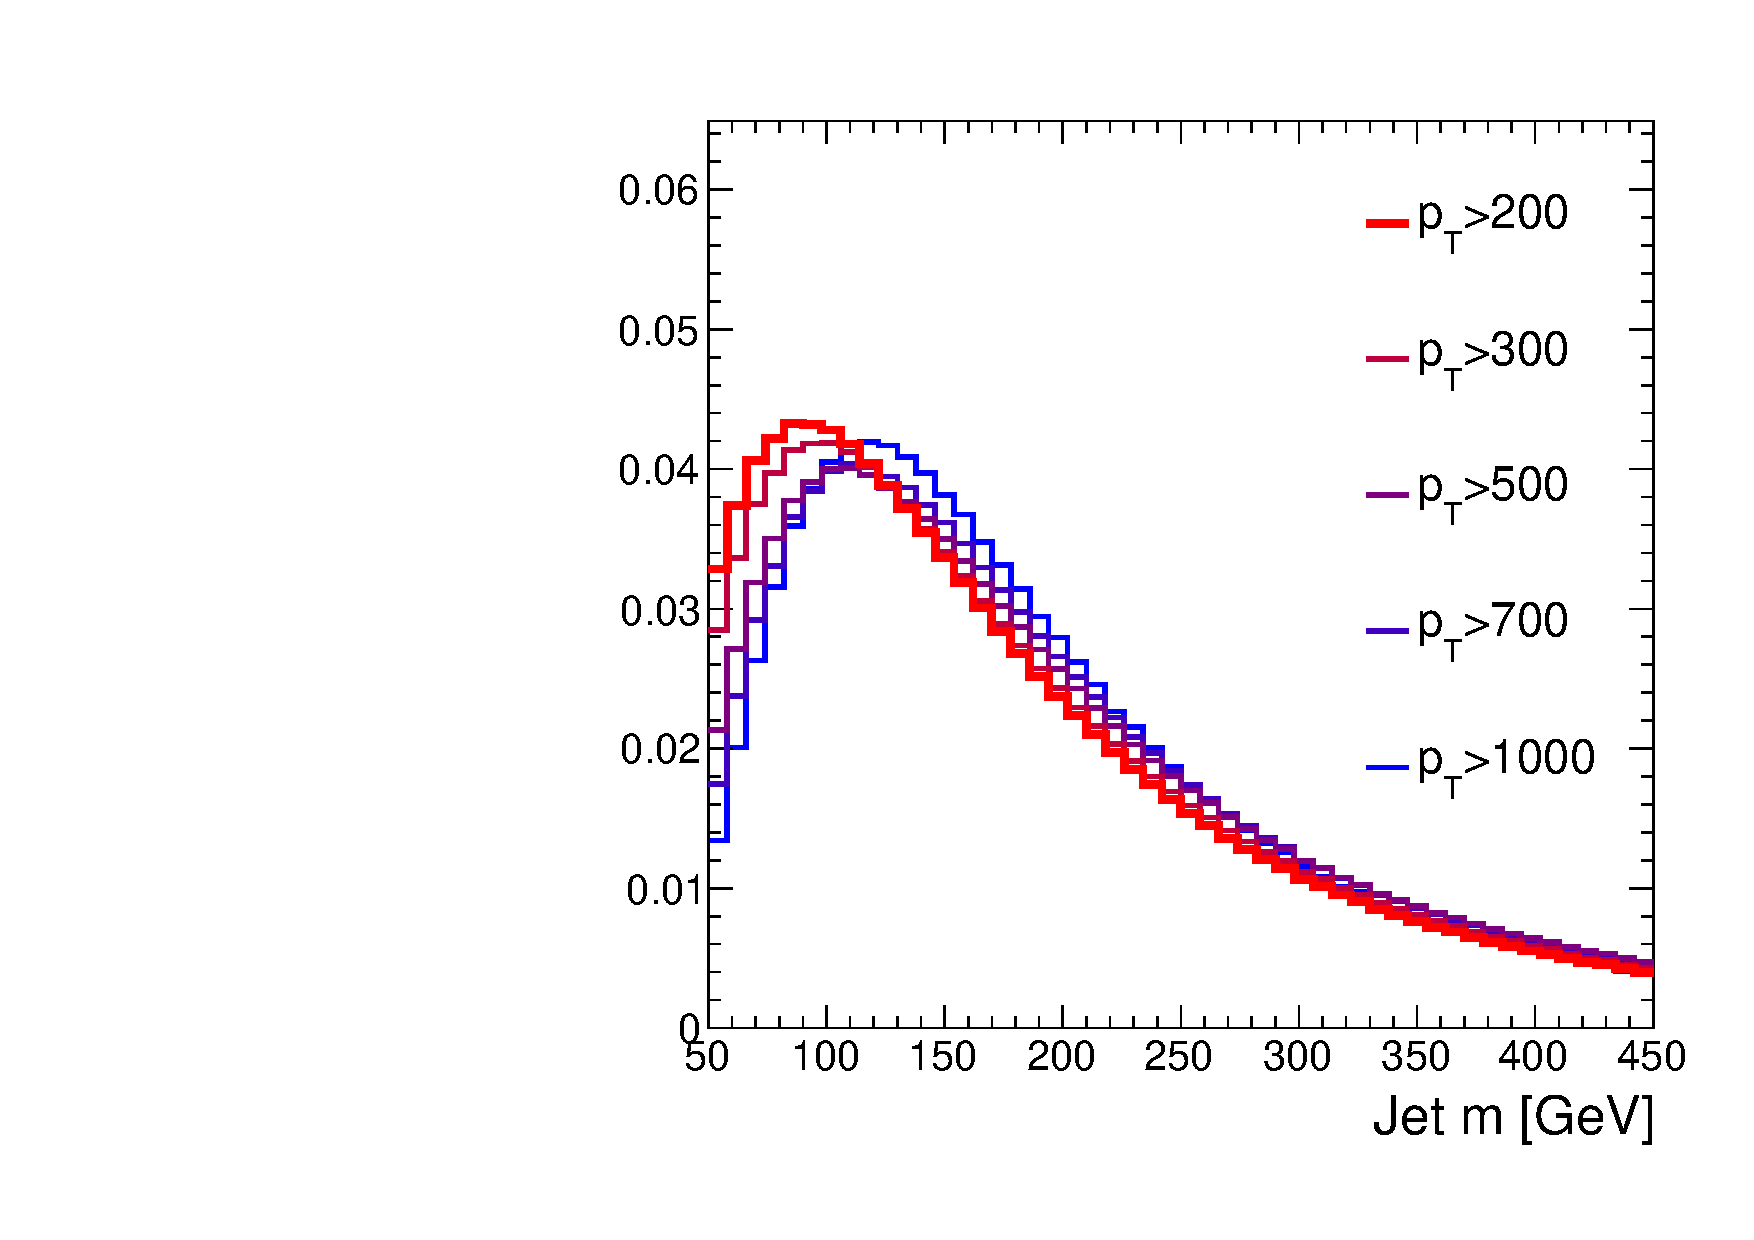
\includegraphics[width=\textwidth]{figures/toptagging/gen/norm_clf_M_QCD.pdf}
            \caption{Ungroomed, LQG}
        \end{subfigure}
        \begin{subfigure}[t]{0.35\textwidth}
            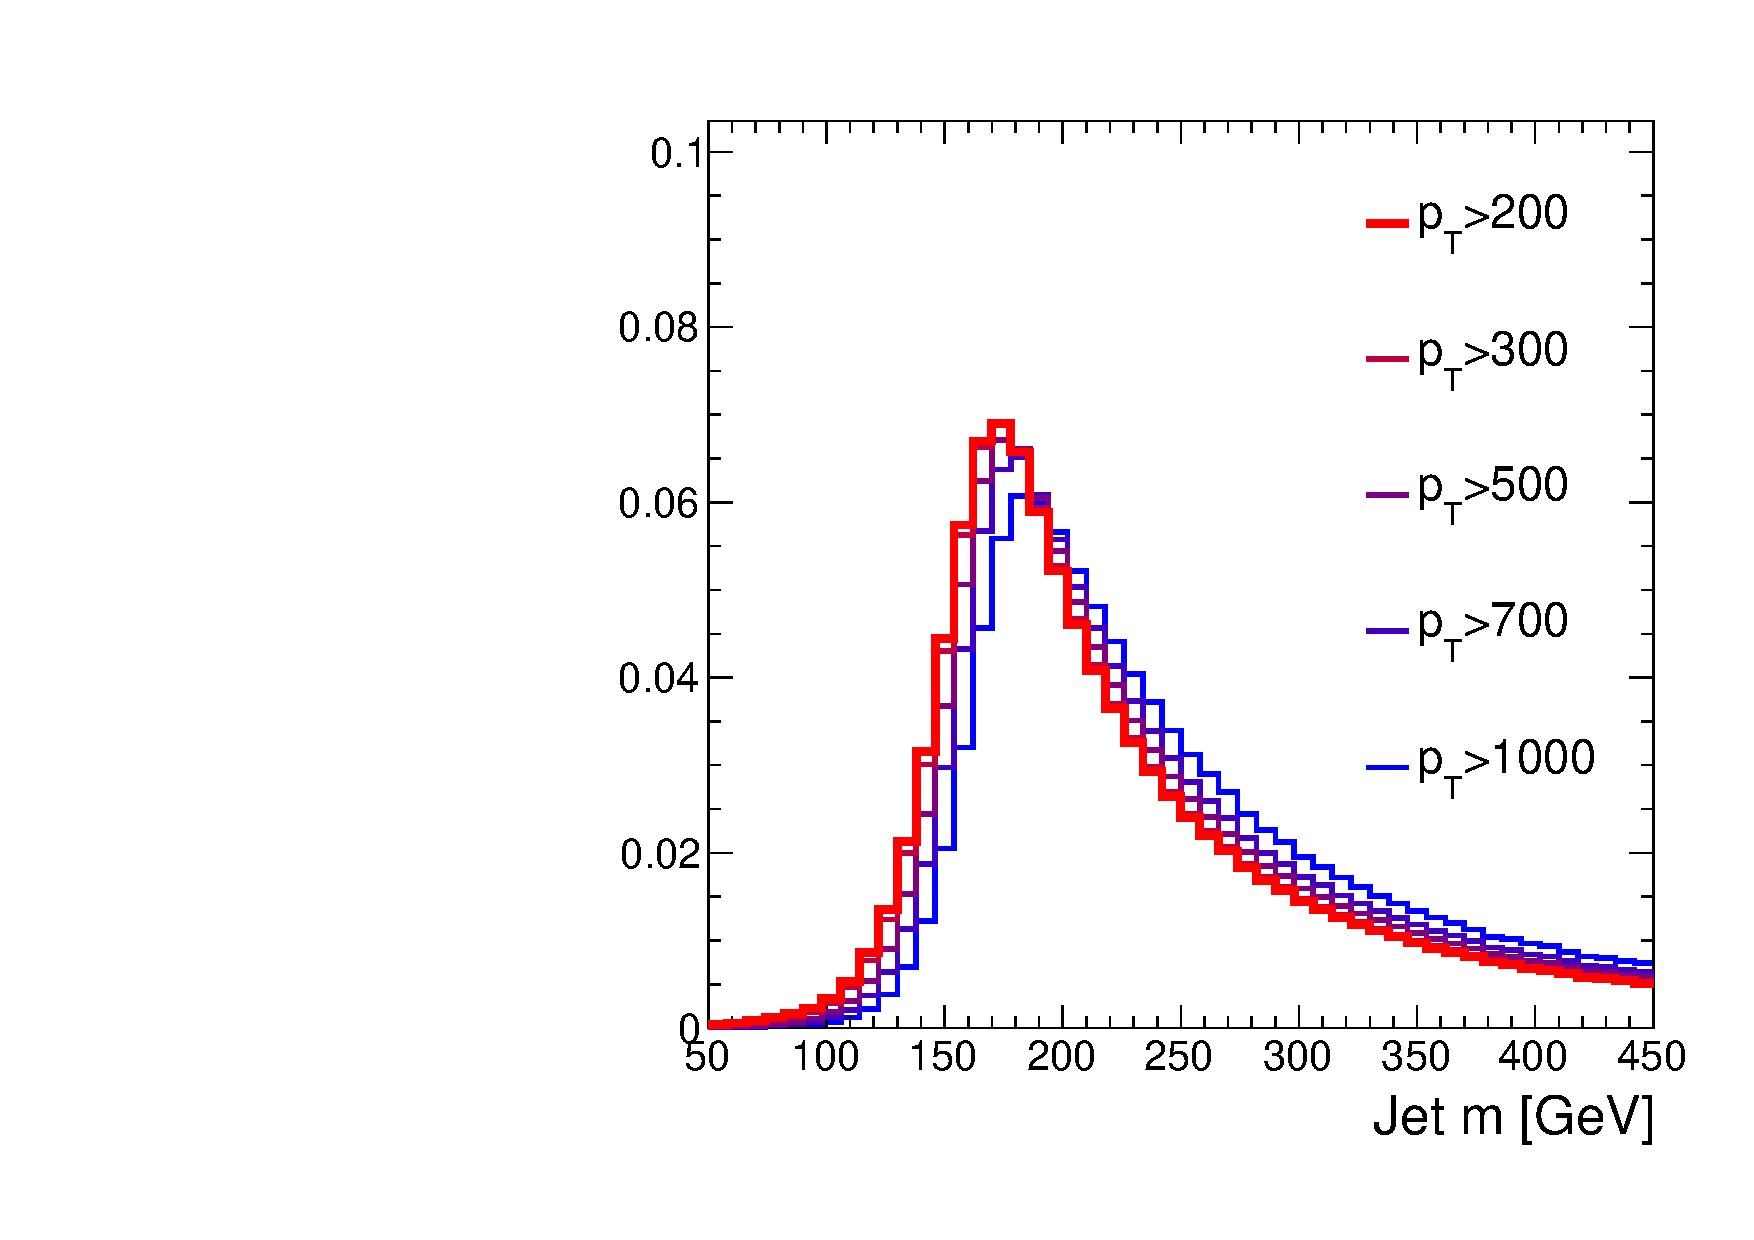
\includegraphics[width=\textwidth]{figures/toptagging/gen/norm_clf_M_ZpTT_lo.pdf}
            \caption{Ungroomed, Top}
        \end{subfigure}
        \begin{subfigure}[t]{0.35\textwidth}
            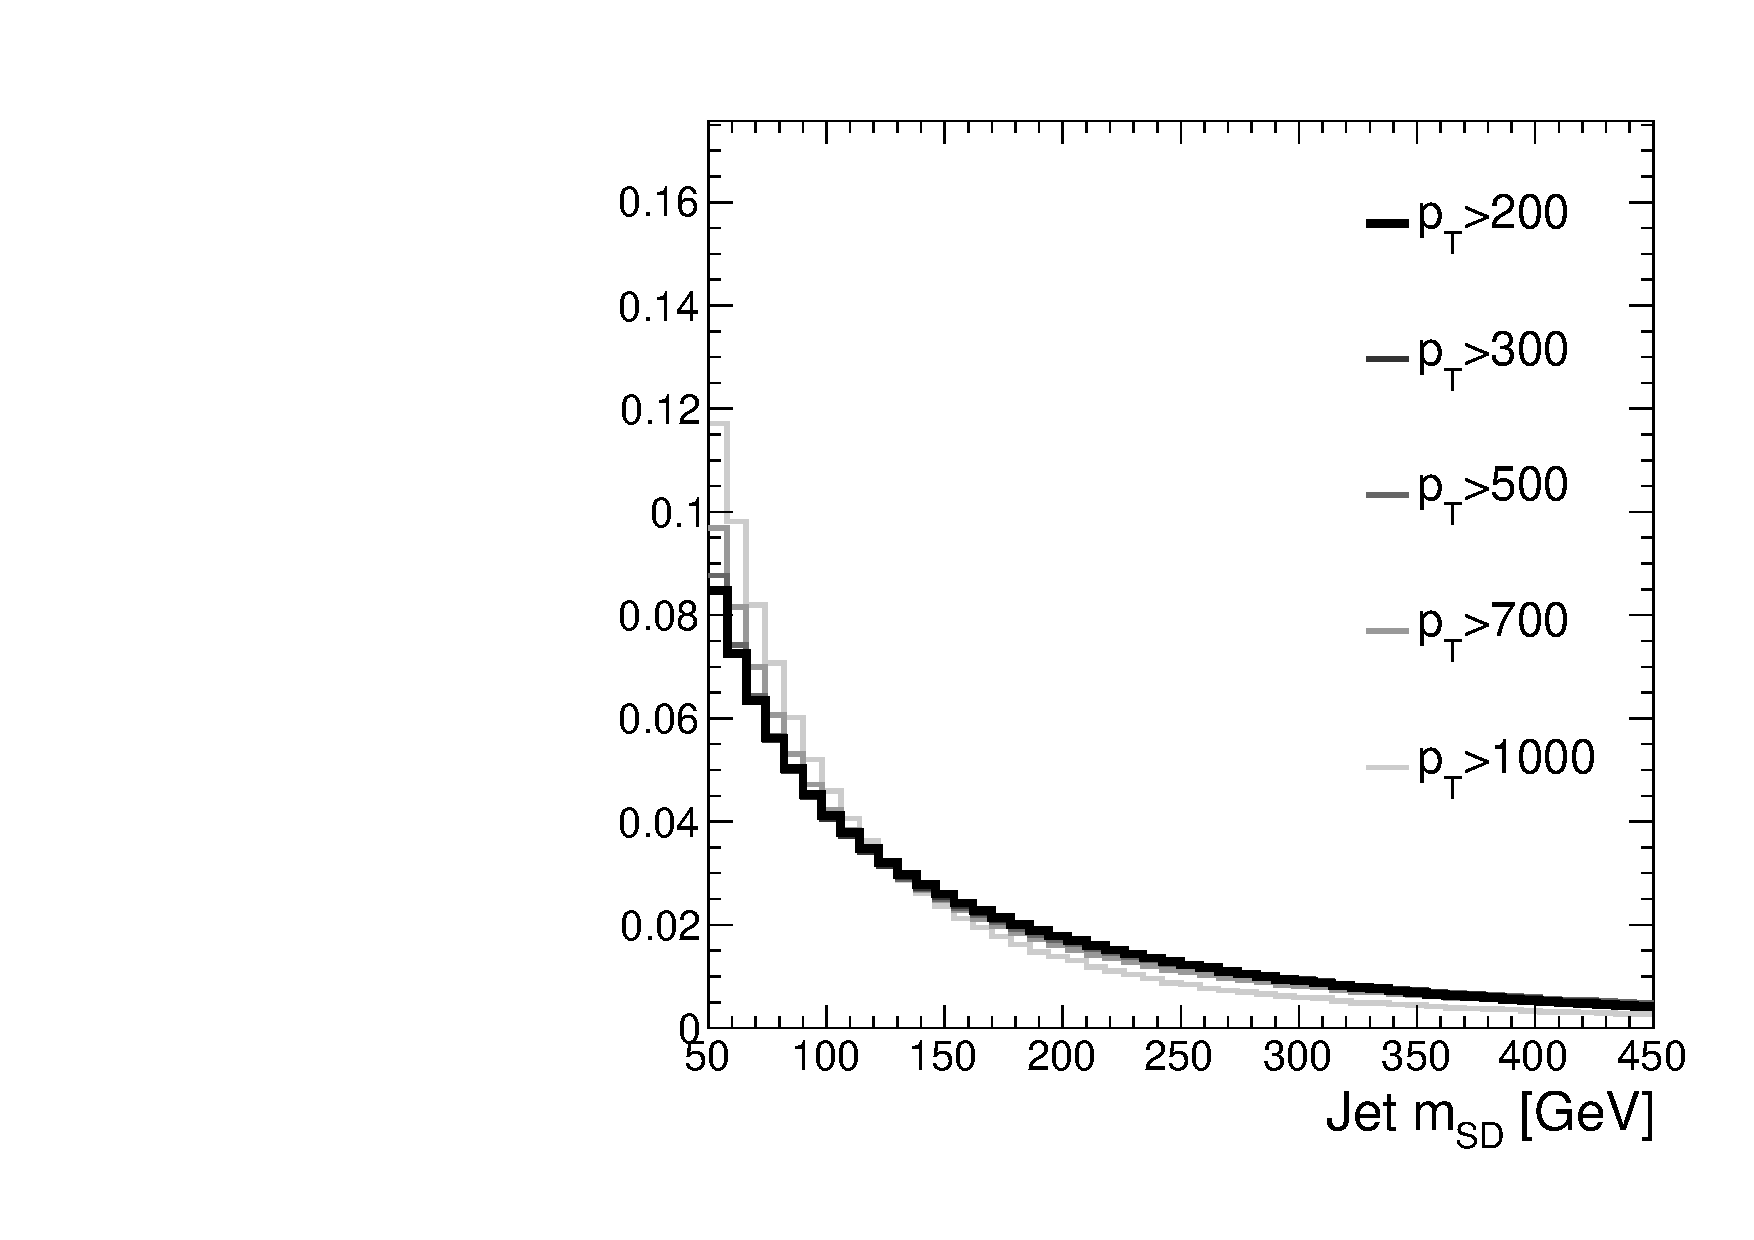
\includegraphics[width=\textwidth]{figures/toptagging/gen/norm_clf_MSD_QCD.pdf}
            \caption{SD, LQG}
        \end{subfigure}
        \begin{subfigure}[t]{0.35\textwidth}
            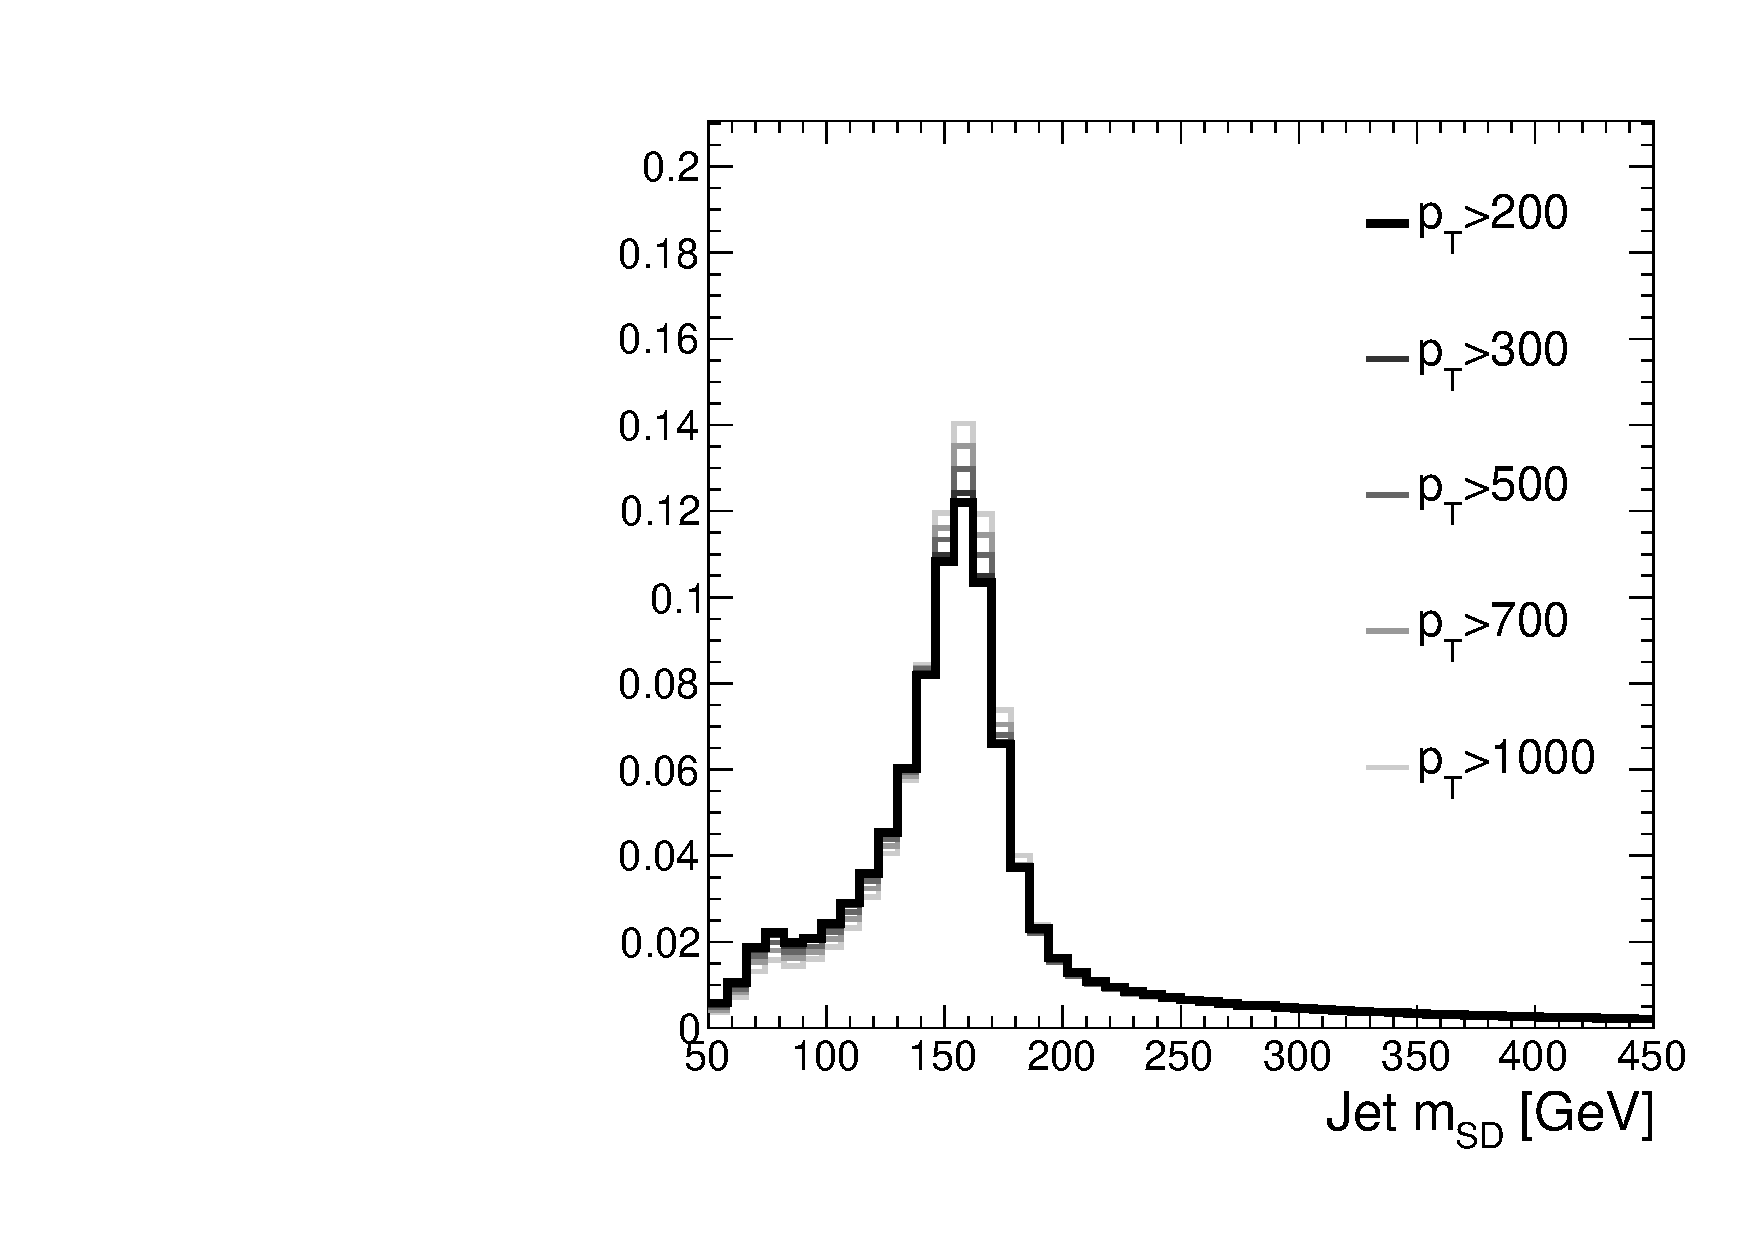
\includegraphics[width=\textwidth]{figures/toptagging/gen/norm_clf_MSD_ZpTT_lo.pdf}
            \caption{SD, Top}
        \end{subfigure}
        \caption{Distribution of ungroomed and groomed jet mass in CA15 jets originating from LQG or hadronic top decays.
                 The multiple histograms represent increasingly stringent \pt~requirements on the parton that initiates the jet.}
        \label{fig:jets:msd}
    \end{center}
\end{figure}

\subsection{Substructure}

A substructure observable is any function of a jet's constituents that is sensitive to the multi-pronged structure of a heavy resonance decay. 
In addition to jet mass and $b$-tagging, substructure is used to reject LQG jets as top decay candidates. 

\subsubsection{$N$-subjettiness}

The $N$-subjettiness ($\tau_N$) is a measure of the compatibility of a jet with an $N$-axis hypothesis~\needcite.
It is defined as:
\begin{equation}
    \tau_N = \frac{\sum_{i\in\mathrm{jet}} p_{\mathrm{T},i} \min\{\Delta R_{ia} | a\in A\}}{\sum_{i\in\mathrm{jet}} p_{\mathrm{T},i} R}
\end{equation}
where $R=1.5$ (the jet radius); $\Delta R_{ia}$ is the $\Delta R$ distance between the particle $i$ and the axis $a$; and $A$ is a set of $N$ axes. 
Ideally, $A$ would be defined to be the set of axes that minimize $\tau_N$ for each jet, but this minimization problem is computationally difficult.  
Instead, the exclusive \kt~algorithm is used to partition the jet's constituents into $N$ subjets (NB: these are not the SD subjets discussed above).
Since the \kt~distance metric is proportional to $\nicefrac{\Delta R^2}{R^2}$, this approximates the ideal minimization.
The set of axes $A$ is taken to be the directions of the $N$ \kt~subjets. 
A small $\tau_N$ indicates a high degree of compatibility with the $N$-axis hypothesis.
Therefore, we expect a 3-pronged (e.g. top) jet to satisfy $\tau_3 \ll \tau_2$, whereas a 1-pronged (e.g. LQG) jet should satisfy $\tau_3 \lesssim \tau_2$ (for optimal choice of $A$, $N>M \Rightarrow \tau_{N} \leq \tau_{M}$ for any jet). 
Correspondingly, we take $\tau_{32} \equiv \nicefrac{\tau_3}{\tau_2}$ to be the tagging observable. 

Figure~\ref{fig:jets:tau32} shows the distribution of $\tau_{32}$.
As with jet mass, we may calculate $\tau_{32}$ either on the whole jet or on the groomed (SD) jet.
The discrimination between top and LQG jets is similar in both cases, but as Figure~\ref{fig:jets:msdtau} demonstrates, $\tau_{32}^\SD$ has the weaker correlation with $m_\SD$ in LQG jets. 
This feature will be critical to validate any tagger in data, as described in Section~\ref{sec:jets:sf}.

\begin{figure}[]
    \begin{center}
        \begin{subfigure}[t]{0.32\textwidth}
            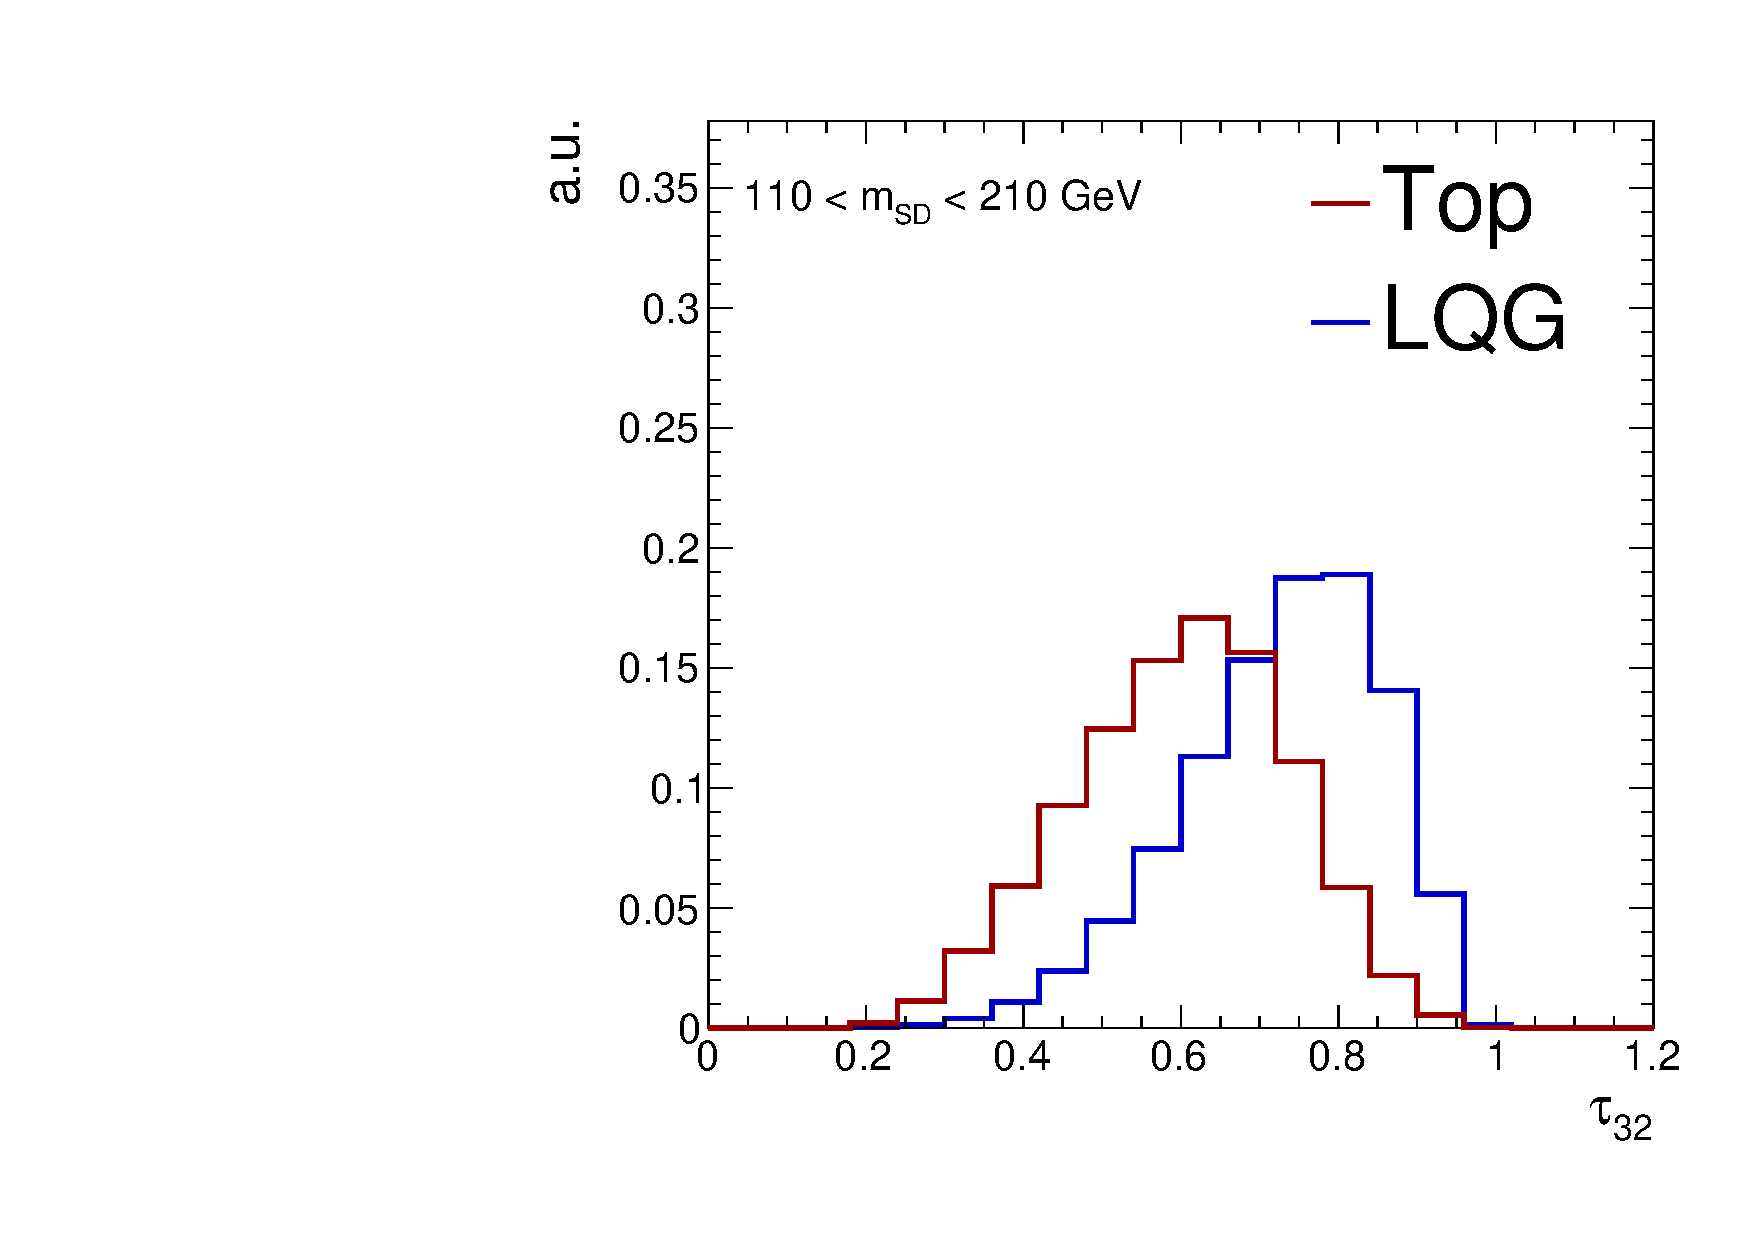
\includegraphics[width=\textwidth]{figures/toptagging/shapes/mass_fjTau32.pdf}
            \caption{}
        \end{subfigure}
        \begin{subfigure}[t]{0.32\textwidth}
            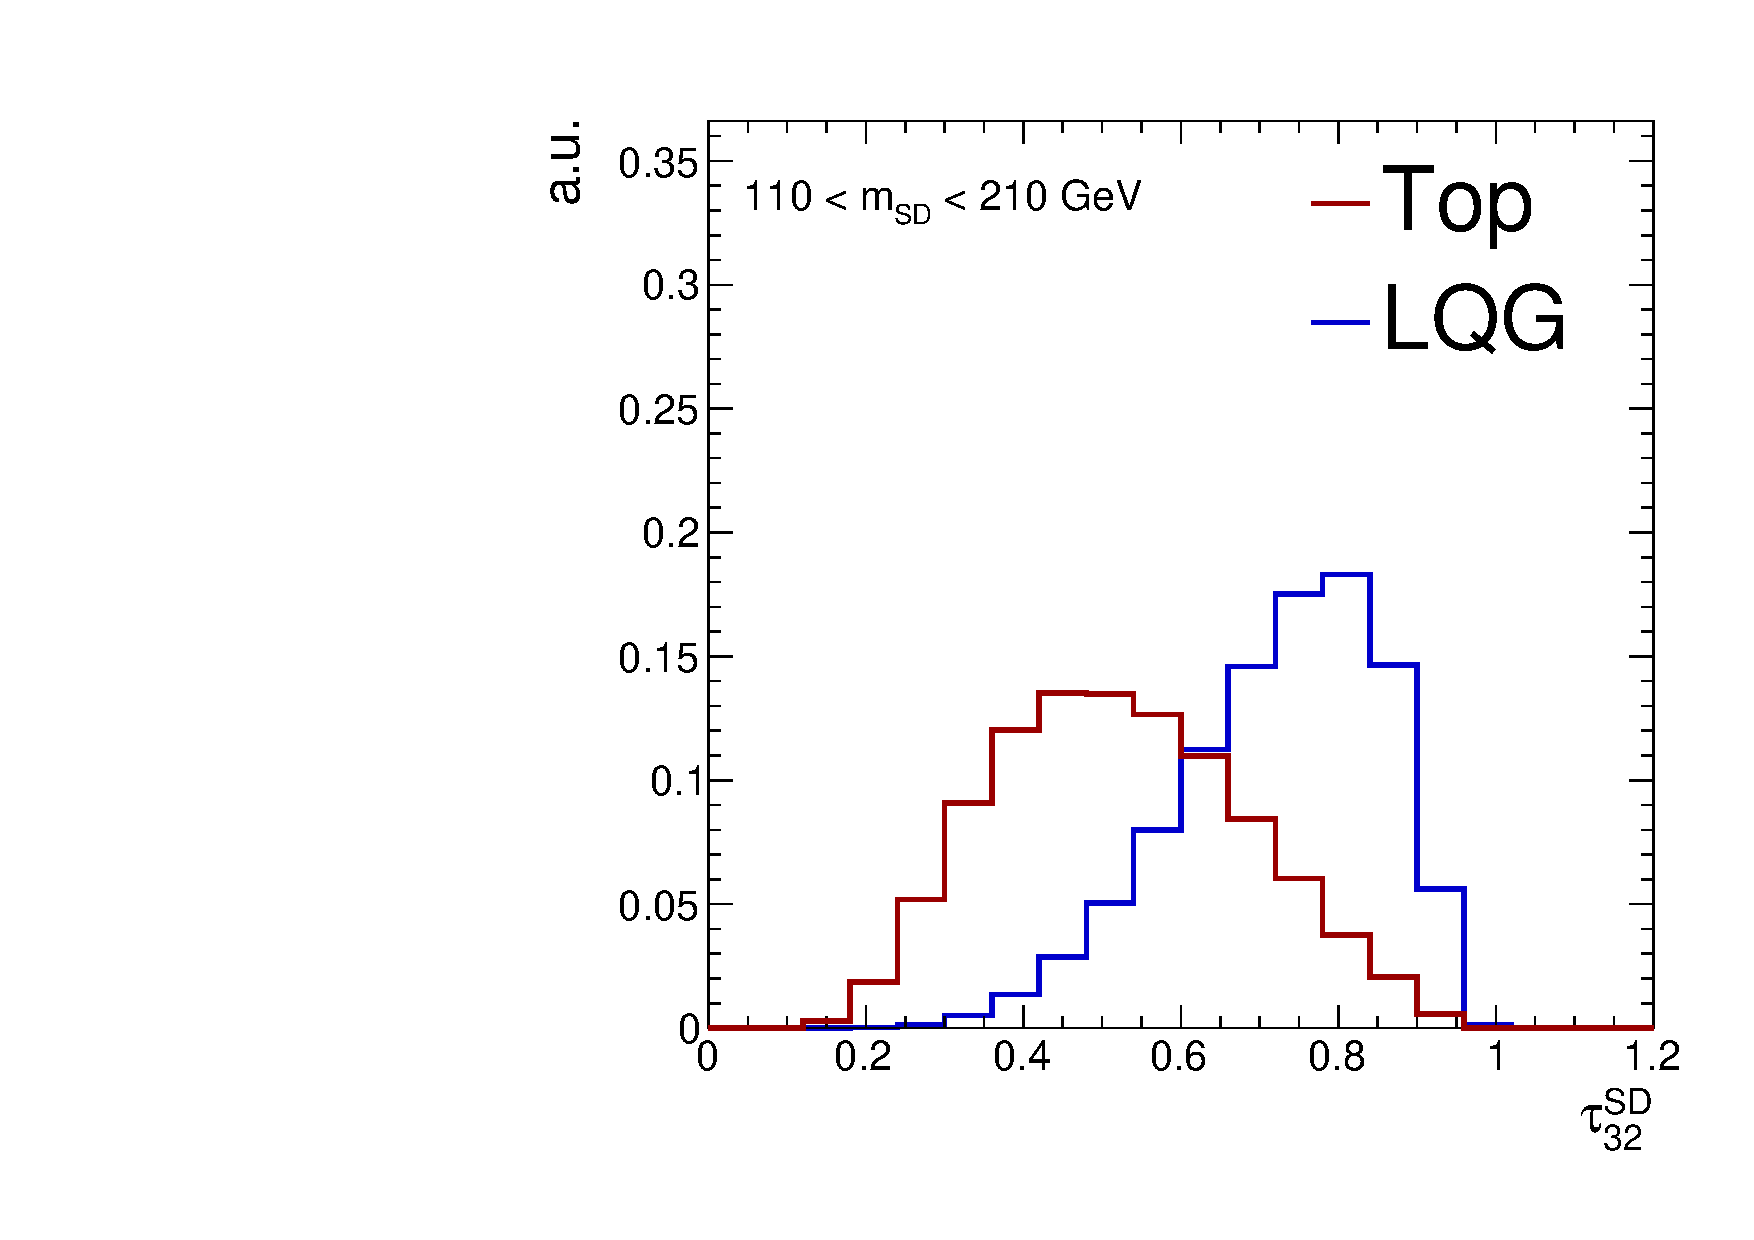
\includegraphics[width=\textwidth]{figures/toptagging/shapes/mass_fjTau32SD.pdf}
            \caption{}
        \end{subfigure}
        \begin{subfigure}[t]{0.32\textwidth}
            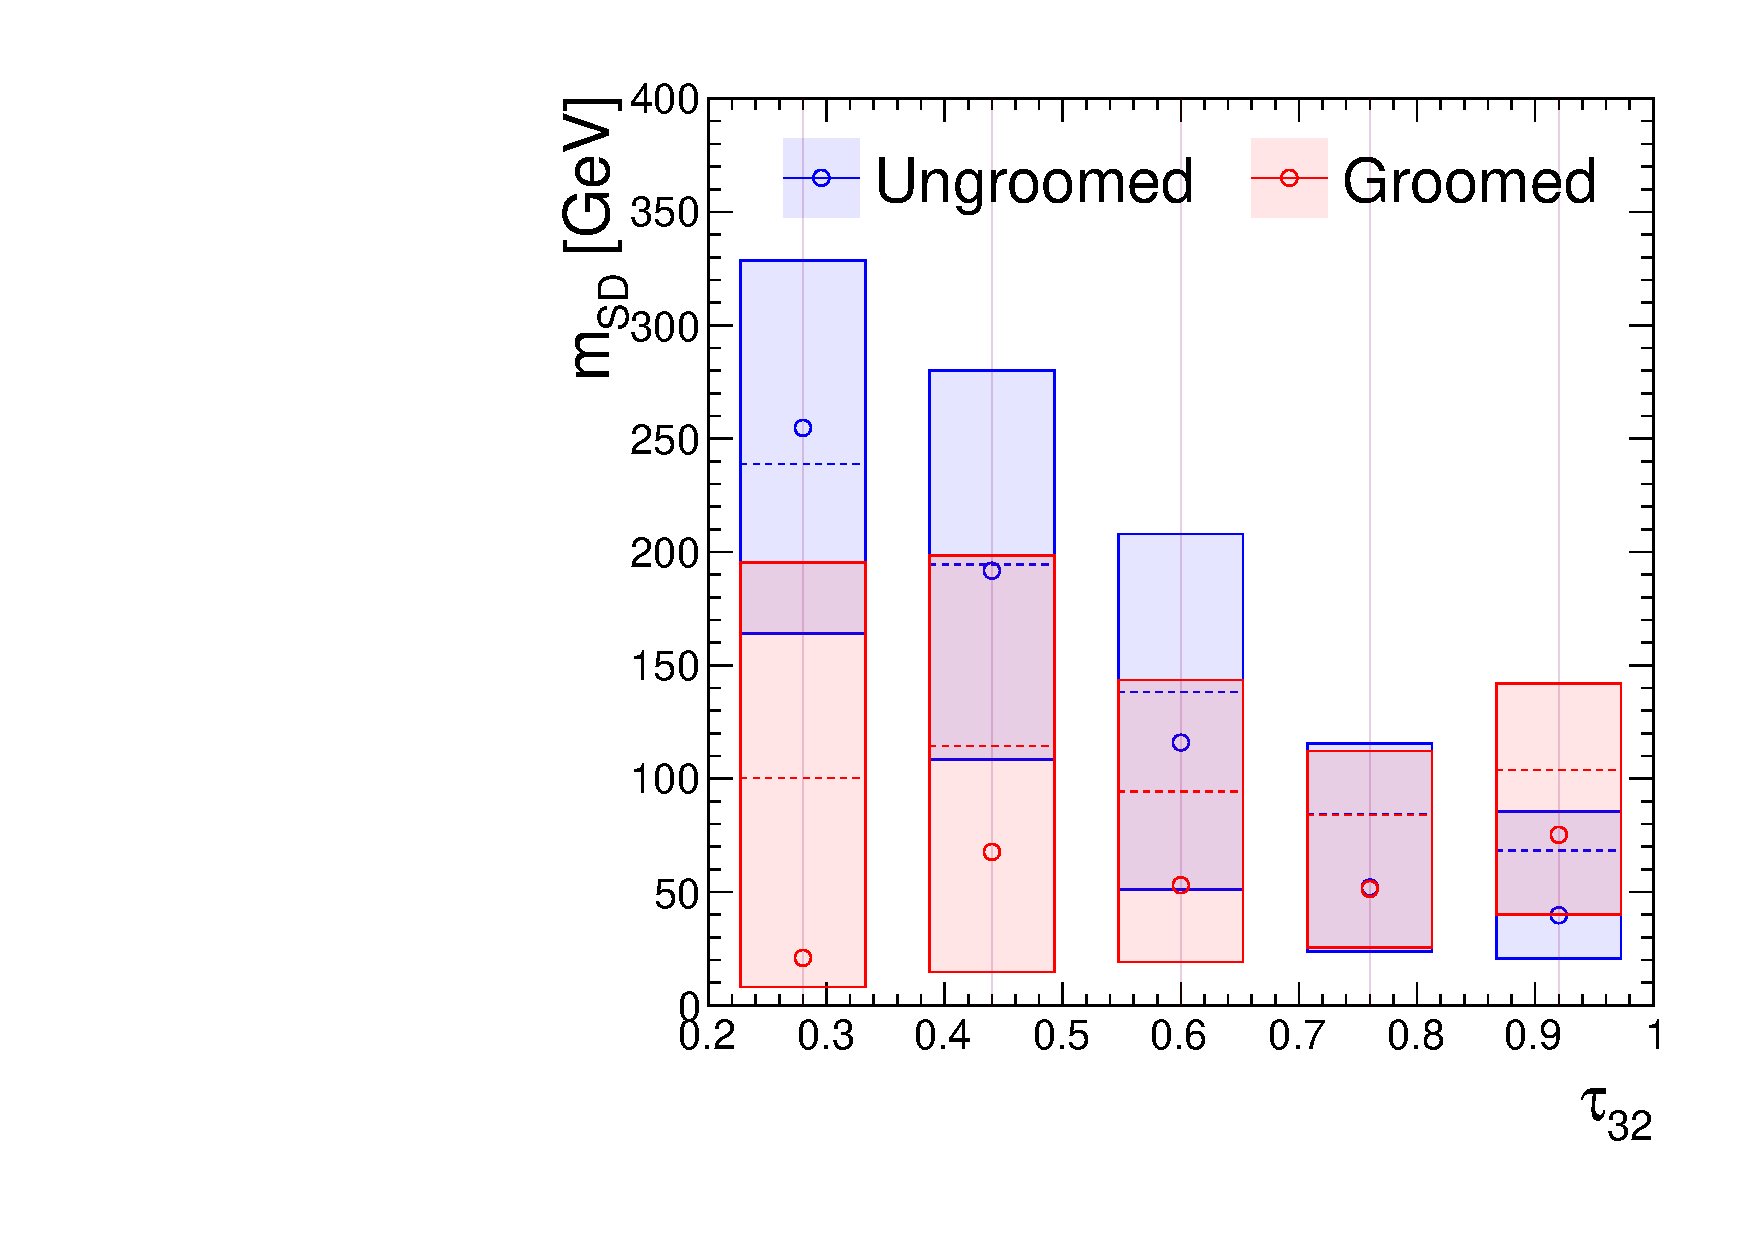
\includegraphics[width=\textwidth]{figures/toptagging/gen/msdtau_QCD.pdf}
            \caption{}
            \label{fig:jets:msdtau}
        \end{subfigure}
        \caption{Shape of ungroomed (left) and groomed (center) $\tau_{32}$ distributions in top and LQG jets, with a mass selection consistent with $m_t$. 
                 Right: the correlation between $\tau_{32}$ and $m_\SD$ in LQG jets, comparing groomed and ungroomed jets. 
                 }
        \label{fig:jets:tau32}
    \end{center}
\end{figure}

\subsubsection{\HTT}
% https://arxiv.org/pdf/1503.05921.pdf

The \HTT~algorithm de-clusters the jet into many subjets and attempts to reconstruct the $W$ and $t$ decay products out of these subjets~\needcite.
The computation of the tagging variable \frec~can be simplified into three steps (a more detailed description is found in the appendix of Reference~\needcite):
\begin{enumerate}
    \item Compute subjets of the CA15 jet. This is done in a fashion similar to the SD subjets discussed above, but instead of taking the two subjets of the root node, the tree is traversed until some lower \pt~bound is crossed.
    \item Test all triplet combinations of the found subjets and define the $m_{123}$ as the groomed mass of the trijet system. 
    \item Choosing the triplet most consistent with a 3-body top decay (see Equation 12 in Reference~\needcite), define:
        \begin{equation}
            \frec = \min_{0\leq i < j \leq 2} \left|
            \frac{\nicefrac{m_{ij}}{m_{123}}}{\nicefrac{m_W}{m_t}} - 1\right|
        \end{equation}
        where the indices $i,j$ index elements of the selected triplet. 
\end{enumerate}
Figure~\ref{fig:jets:htt} shows the distribution of the selected $m_{123}$ and $\frec$, although we will only use the latter as a tagging observable. 
Note that we do not define distinct groomed and ungroomed versions of these observables, as grooming is intrinsically used in defining the subjets. 

\begin{figure}[]
    \begin{center}
        \begin{subfigure}[t]{0.35\textwidth}
            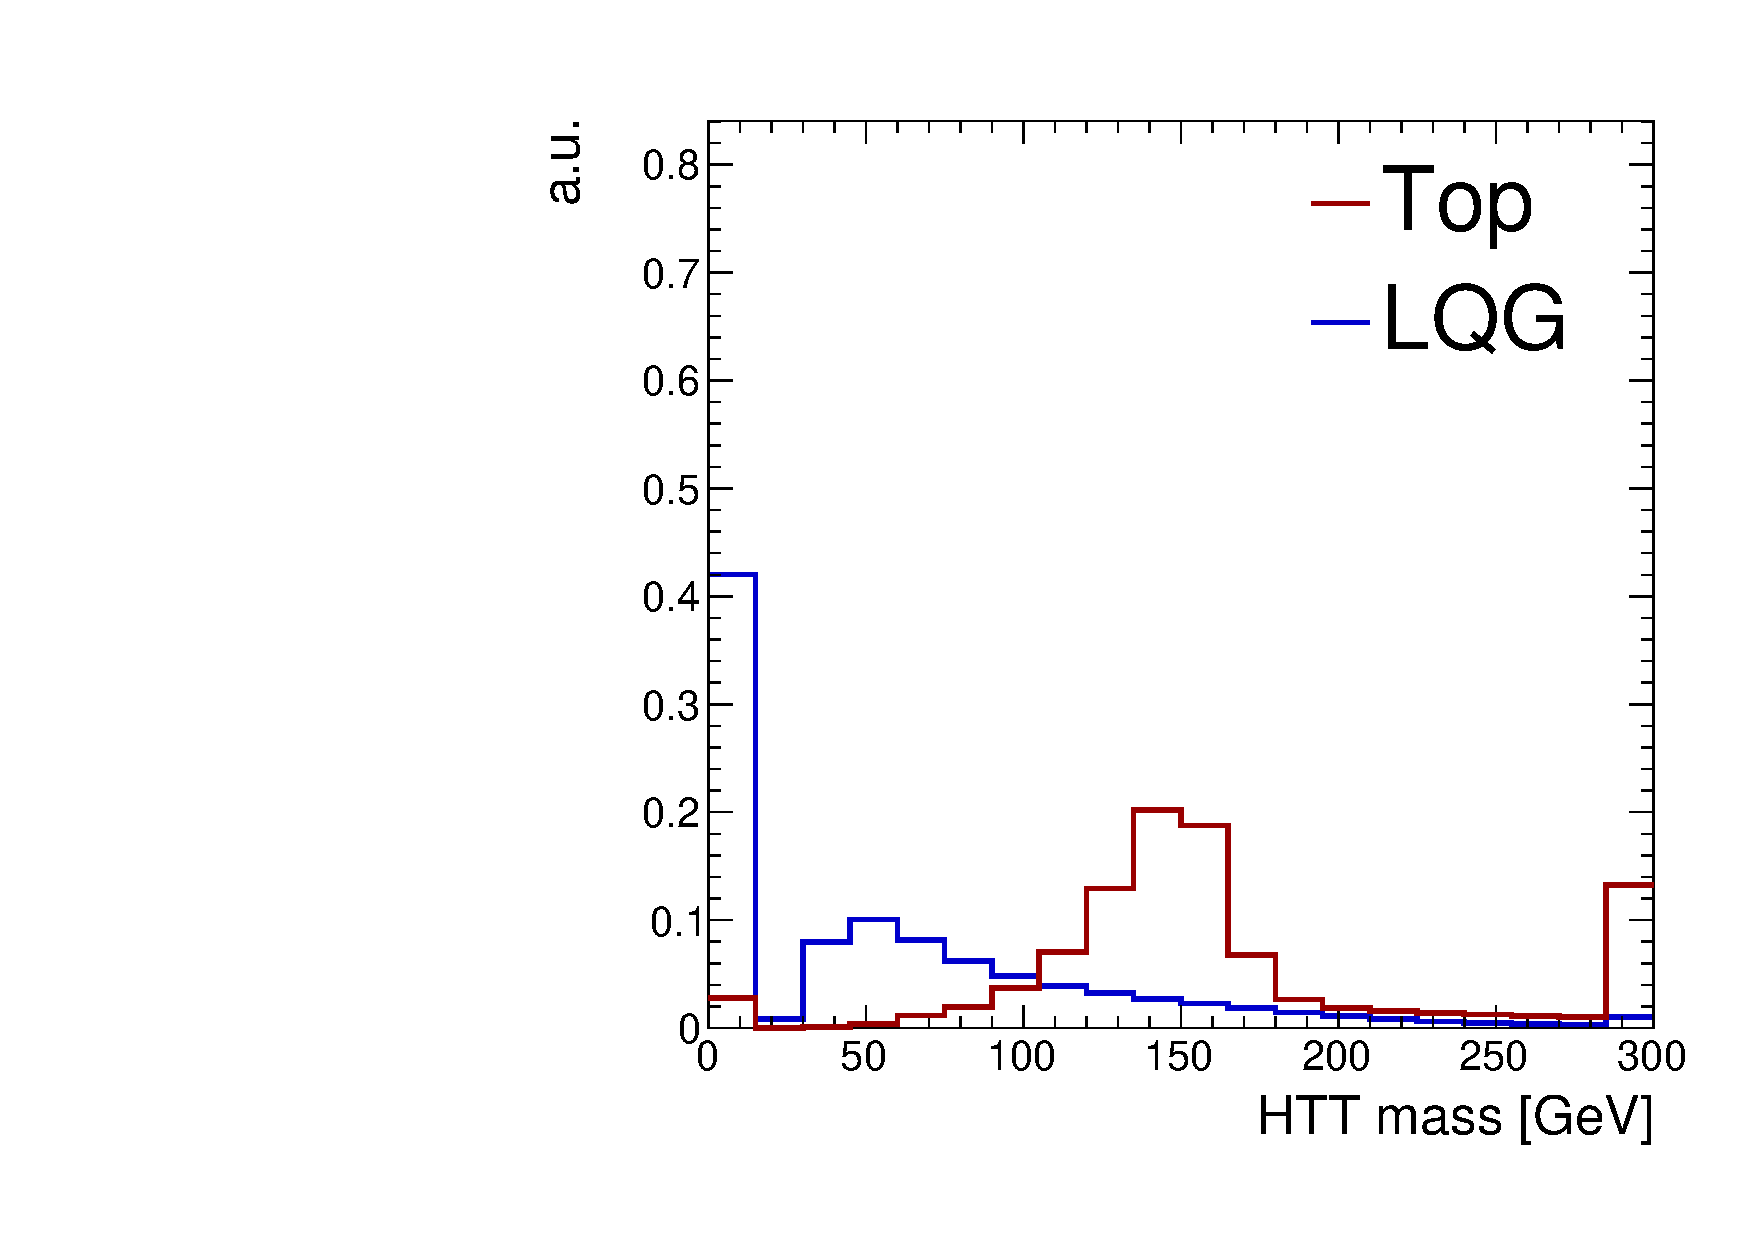
\includegraphics[width=\textwidth]{figures/toptagging/shapes/incl_fjHTTMass.pdf}
        \end{subfigure}
        \begin{subfigure}[t]{0.35\textwidth}
            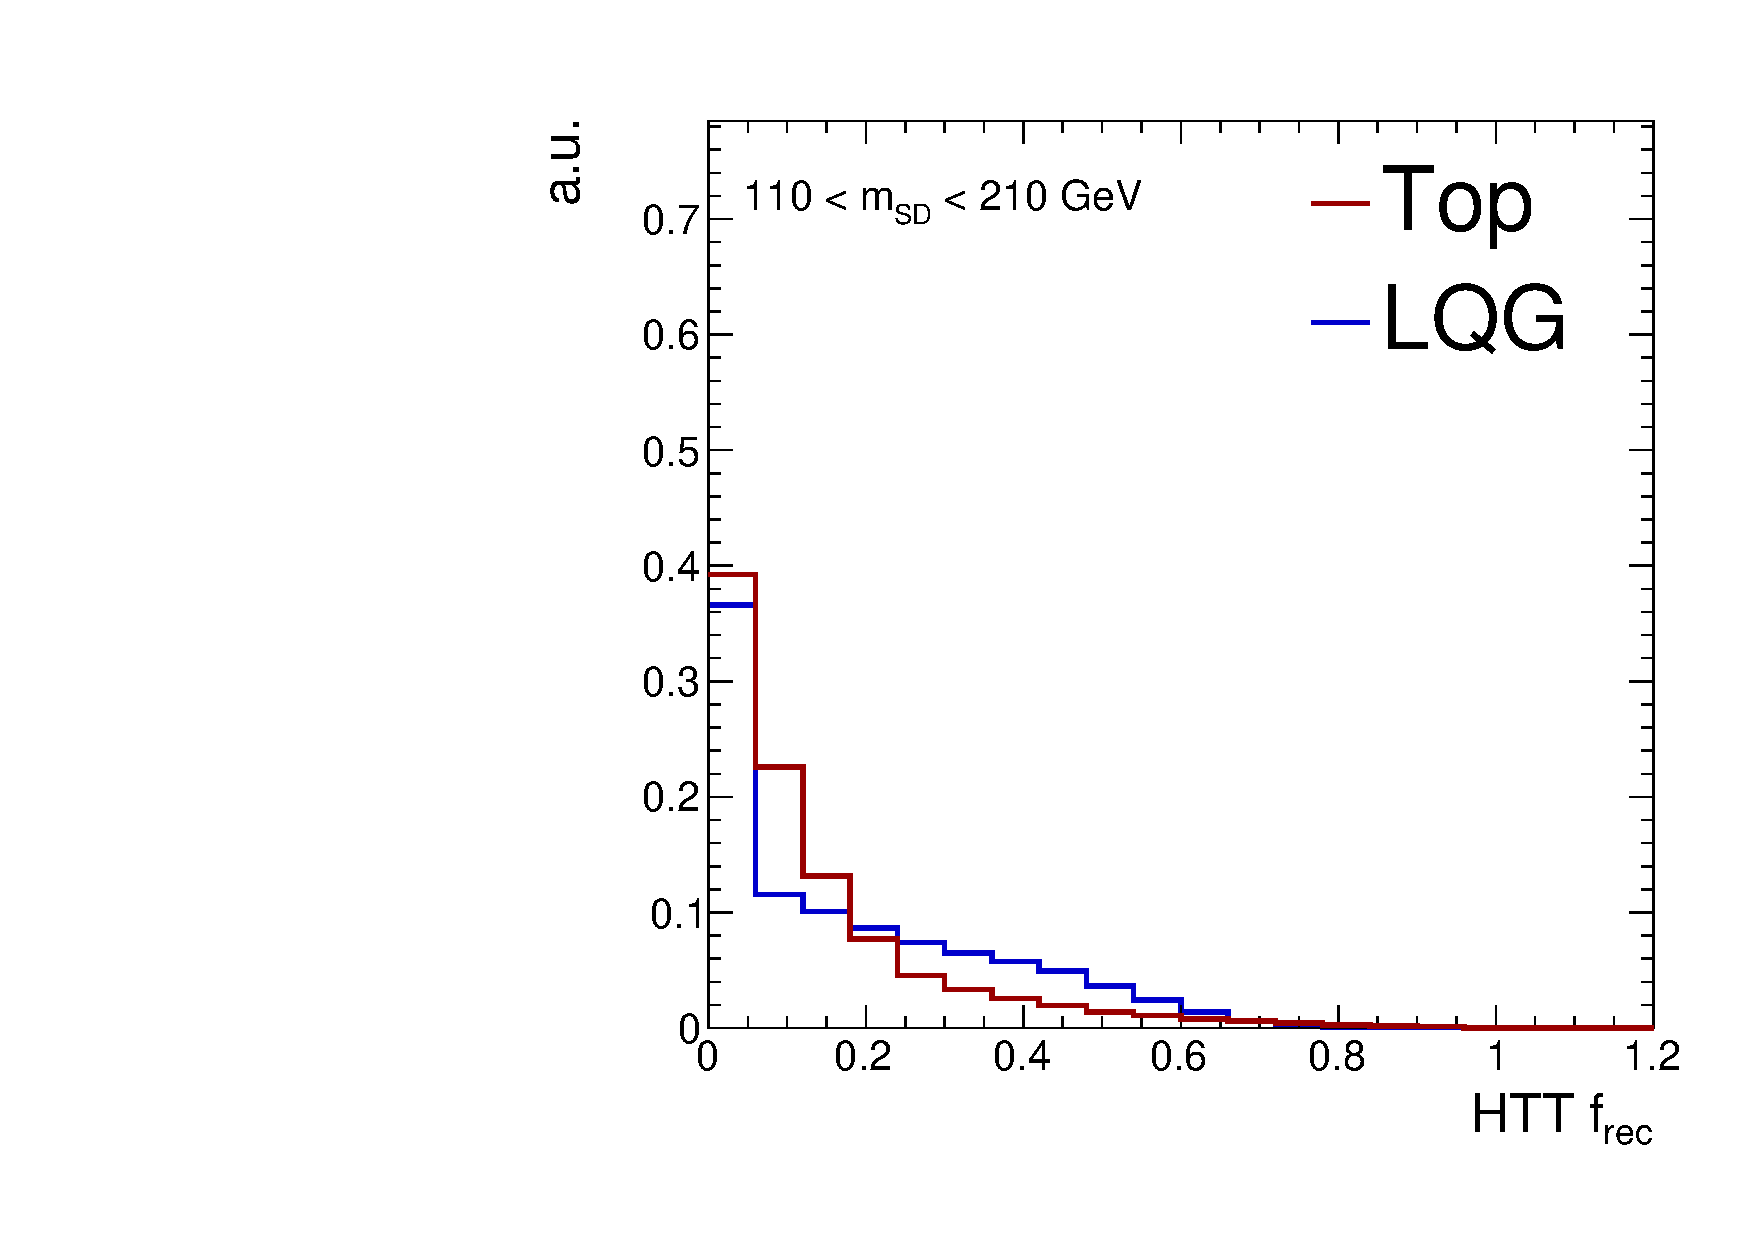
\includegraphics[width=\textwidth]{figures/toptagging/shapes/mass_fjHTTFRec.pdf}
        \end{subfigure}
        \caption{Shape of the $m_{123}$ and $\frec$ observables computed by the \HTT~algorithm. }
        \label{fig:jets:htt}
    \end{center}
\end{figure}

\subsubsection{Energy Correlation Functions}

Energy correlation functions measure the correlation of the positions of hard particles in a jet~\needcite. 
Heuristically, an $N$-point ECF is small if the hard particles can be grouped into fewer than $N$ prongs and large if they arise from $N$ or more prongs. 
An $N$-point ECF, with angular parameters $o$ and $\beta$, is defined as:
\begin{equation}
    e(o,N,\beta) \equiv 
    ~_o e_N^\beta = 
    \sum _{K\subset J, |K|=N} 
    \left[\prod_{i\in K} \frac{\pt^{(i)}}{\pt^{(J)}}\right] \times 
    \min\left\{ \prod_{i,j\in P} \Delta R_{ij}^\beta 
        ~\Big|~ P \subset (K^2 \backslash (k,k)),~|P|=o\right\}
\end{equation}
where $K^2\backslash(k,k)$ indicates all pairs of distinct particles in $K$. 
The proposed tagger in Reference~\needcite~is:
\begin{equation}
    N_3^{(\beta)} = \frac{e(2,4,\beta)}{(e(1,3,\beta))^2}
\end{equation}
Figure~\ref{fig:jets:n3} shows $N_3$ for various values of $\beta$; given our desire for stability as a function of jet \pt~and mass, we only consider ECFs computed on the SD jet. 
The discrimination power of this ECF ratio is roughly comparable to that of $\tau_{32}^\SD$. 
$N_3$ is motivated by the behavior of 3- and 4-point ECFs in top and LQG jets:
\begin{itemize}
    \item In top jets, $e(N=4) \ll e(N=3)$, since 3-point correlation functions are large in a 3-pronged jet
    \item In QCD jets, $e(N=3) \sim e(N=3)$, since both 3- and 4-point ECFs are weak in a 1-pronged jet
\end{itemize}
Therefore, taking the ratio $e(N=4)/e(N=3)$ constructs a useful observable. 

\begin{figure}[]
    \begin{center}
        \begin{subfigure}[t]{0.32\textwidth}
            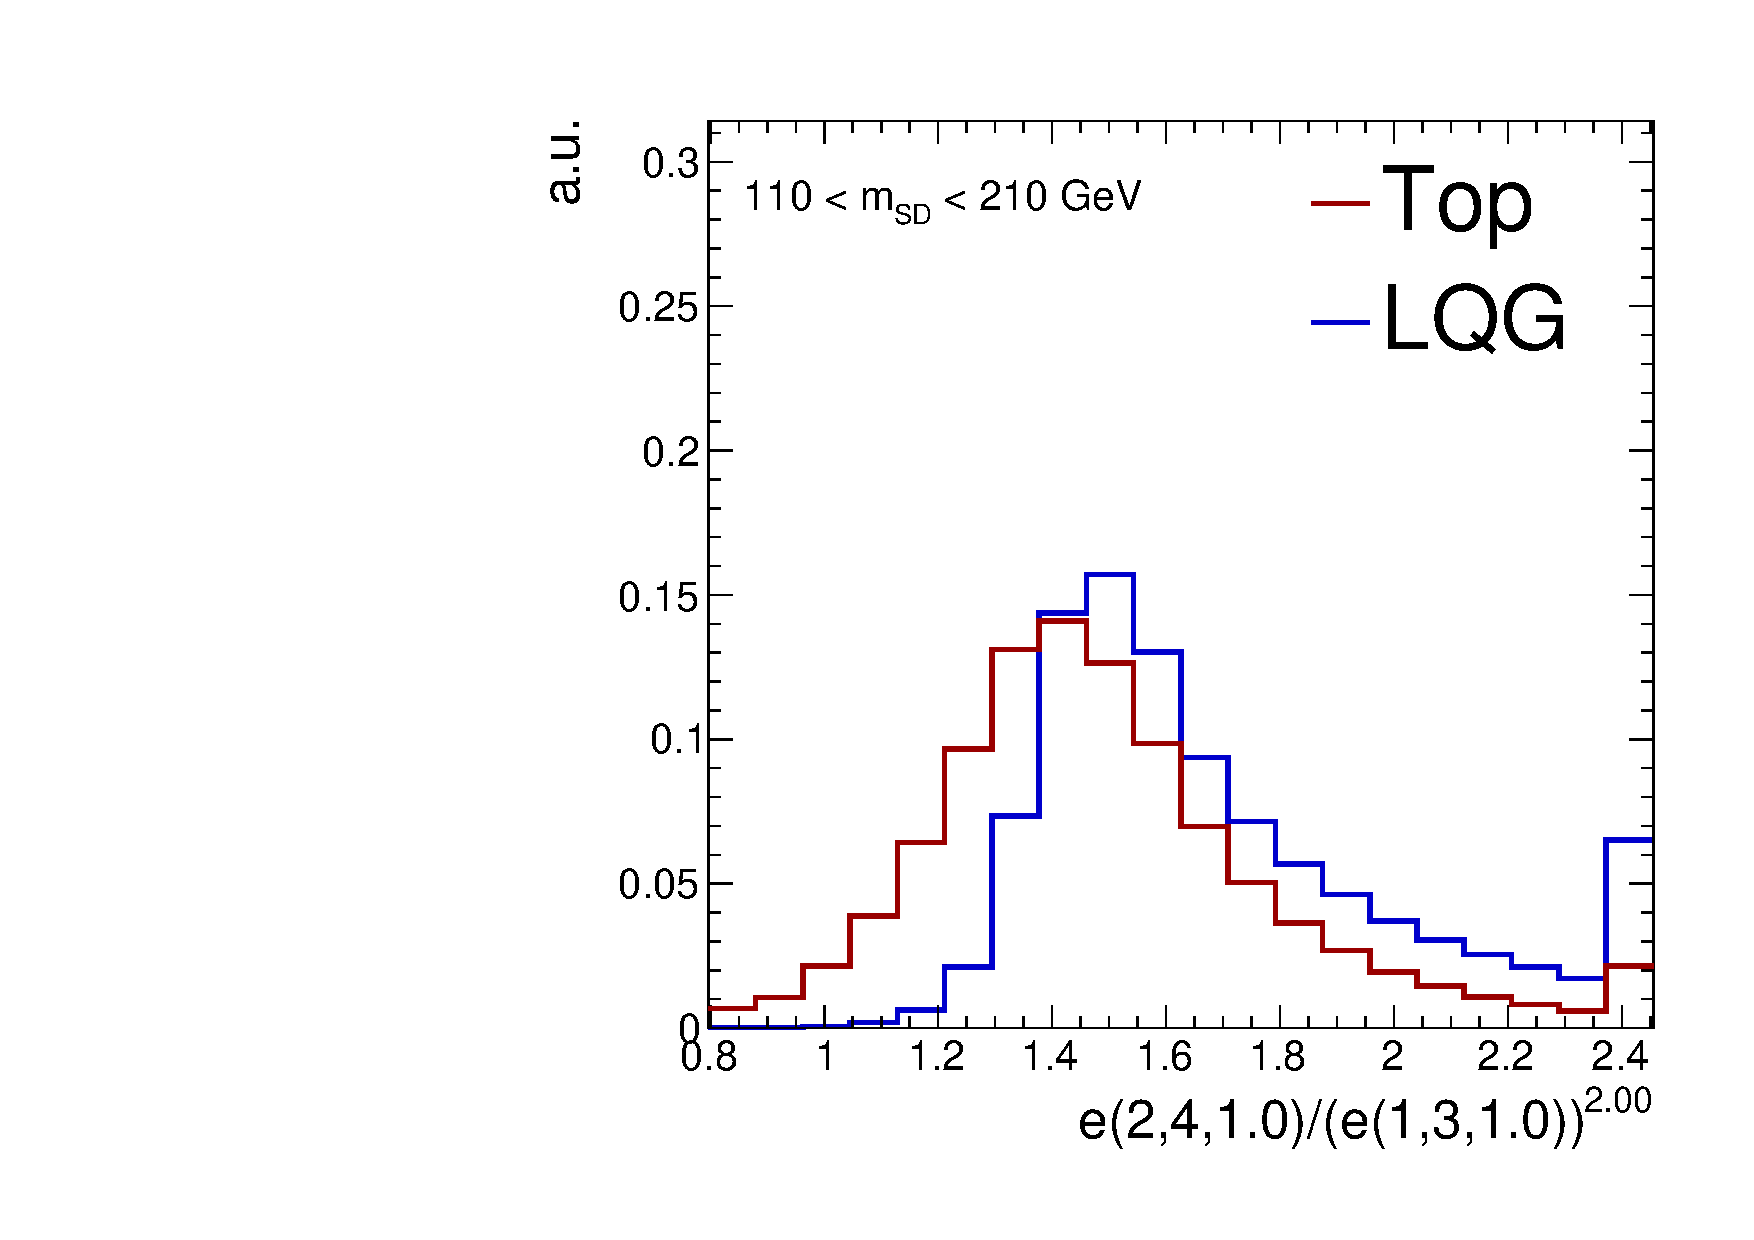
\includegraphics[width=\textwidth]{figures/toptagging/shapes/mass_ratio_24101310.pdf}
        \end{subfigure}
        \begin{subfigure}[t]{0.32\textwidth}
            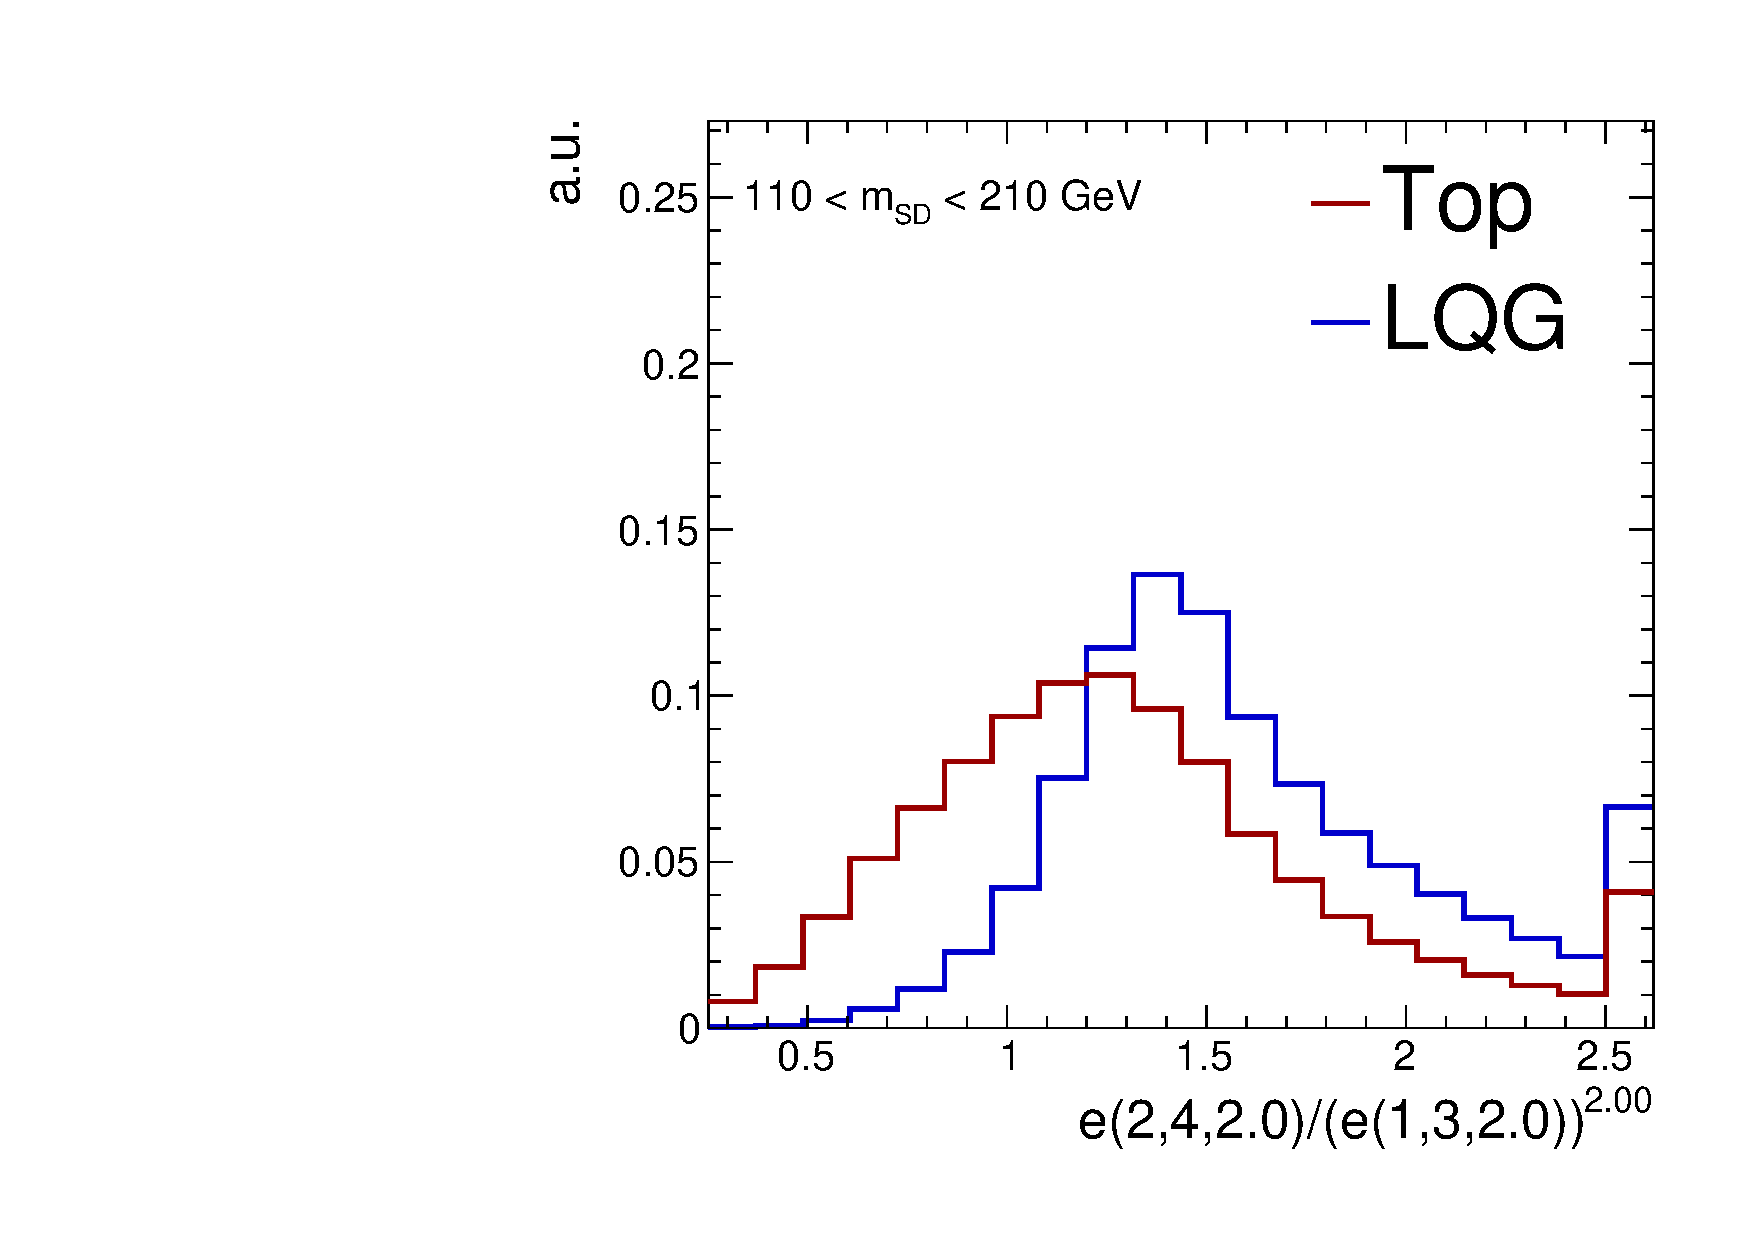
\includegraphics[width=\textwidth]{figures/toptagging/shapes/mass_ratio_24201320.pdf}
        \end{subfigure}
        \begin{subfigure}[t]{0.32\textwidth}
            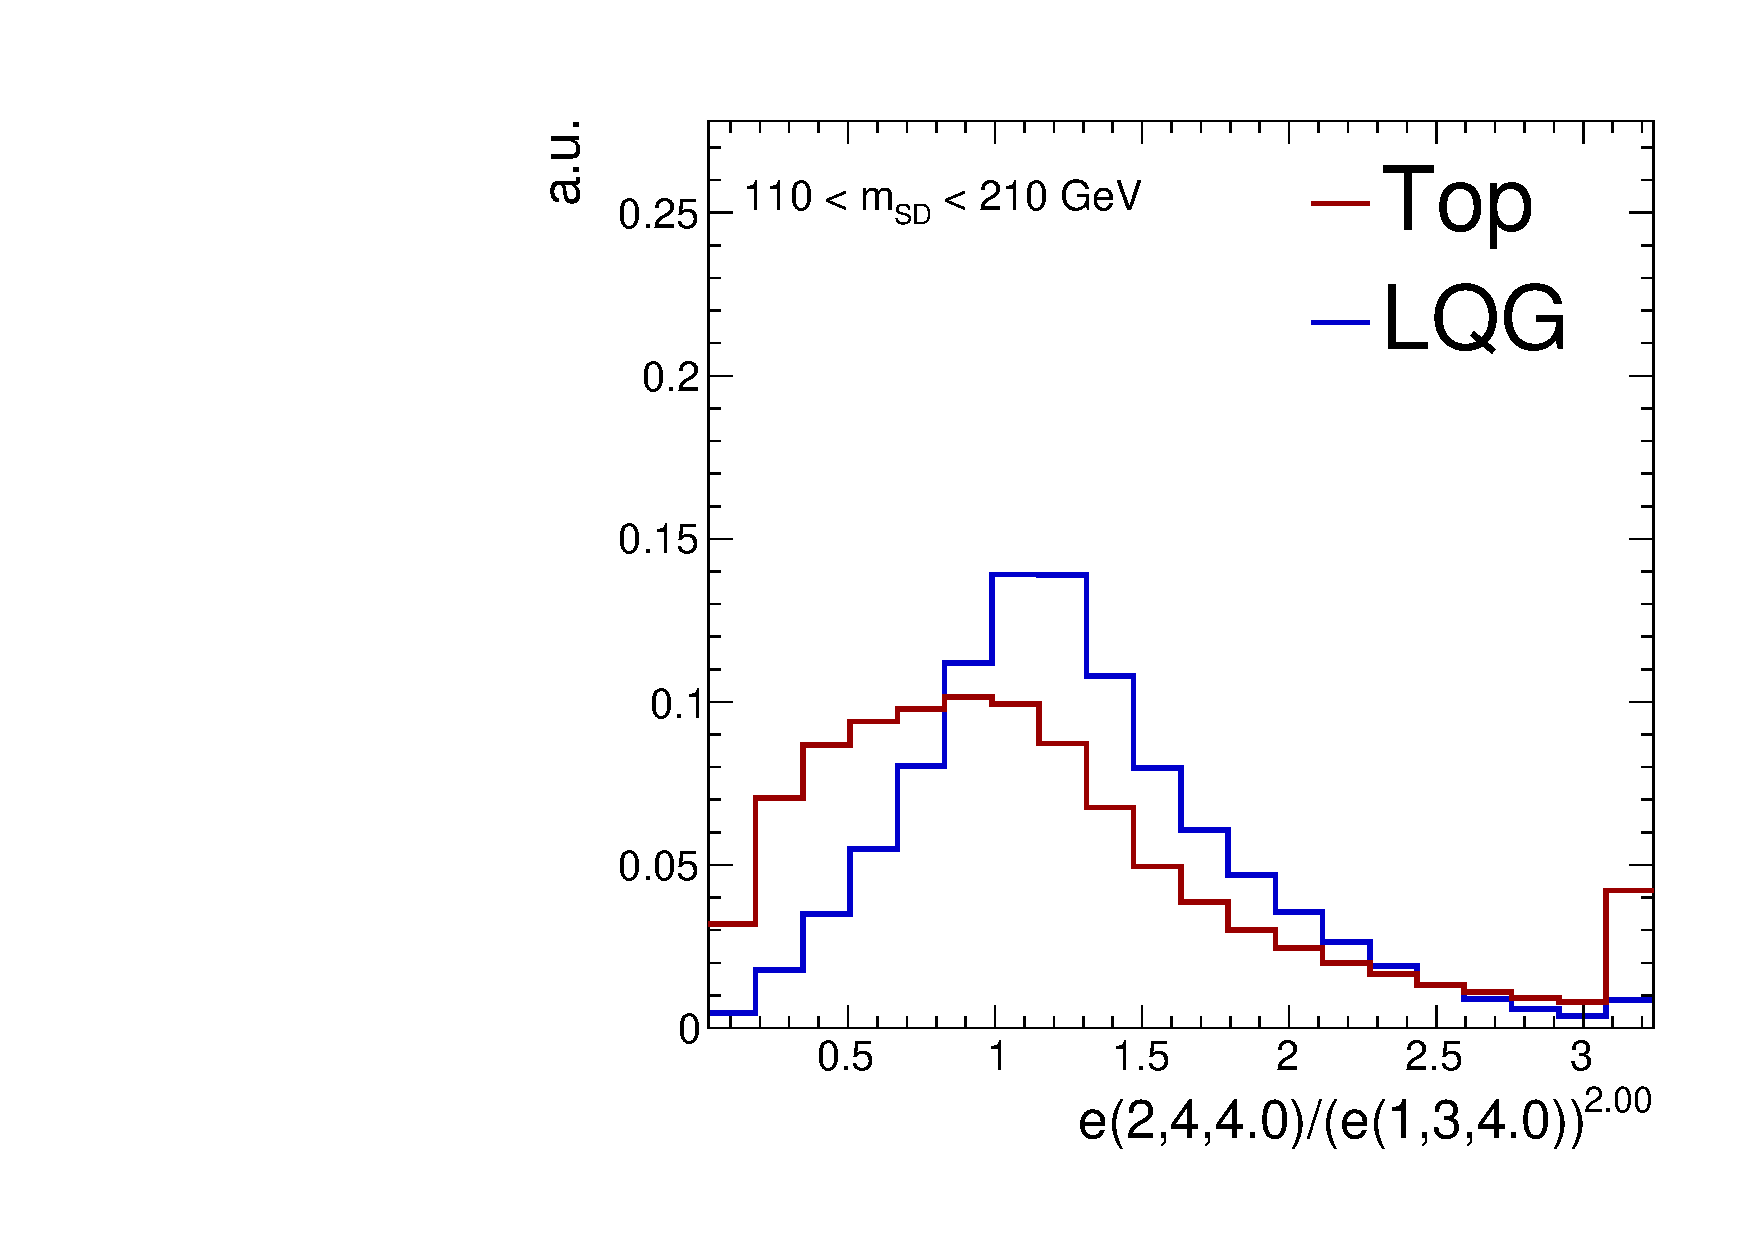
\includegraphics[width=\textwidth]{figures/toptagging/shapes/mass_ratio_24401340.pdf}
        \end{subfigure}
        \caption{Shape of the $N_3$ observables in top and LQG jets, for various values of $\beta$.}
        \label{fig:jets:n3}
    \end{center}
\end{figure}

While $N_3$ has a strong theoretical motivation, it is possible that other functions of ECFs  distinguish between top and LQG jets.
In order to construct observables that do not have a strong dependence on the jet \pt, we restrict ourselves to ratios of the form:
\begin{equation}
    \psi(a,N,\alpha,b,M,\beta) = 
    \frac{e(a,N,\alpha)}{\left(e(b,M,\beta)\right)^x} 
    \text{, where } M\leq N \text{ and } x = \frac{a\alpha}{b\beta}
\end{equation}
A large subset of this broader class of ECF observables are found to be useful (Figure~\ref{fig:jets:ecfrs}), including ratios not of the form $e(N=4)/e(N=3)$.

\begin{figure}[]
    \begin{center}
        \begin{subfigure}[t]{0.32\textwidth}
            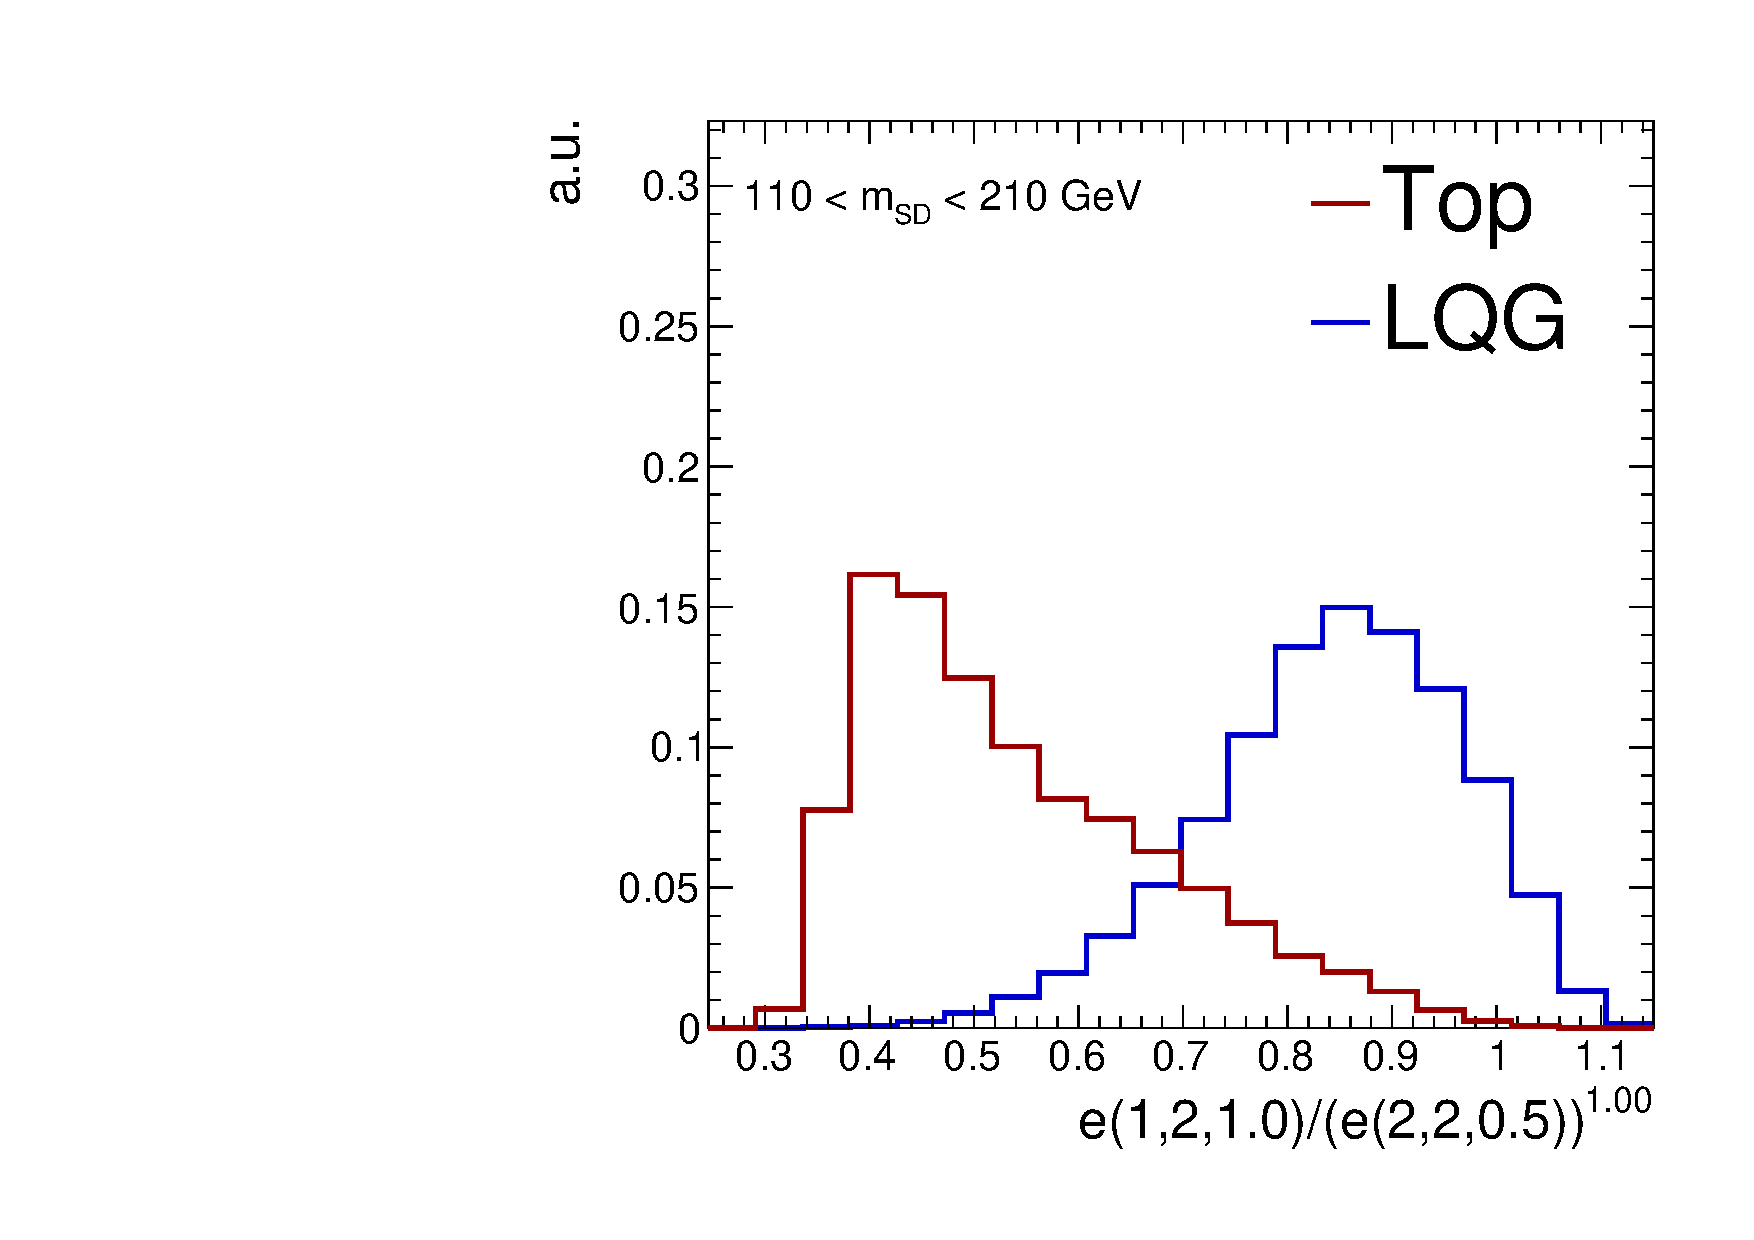
\includegraphics[width=\textwidth]{figures/toptagging/shapes/mass_ratio_12102205.pdf}
        \end{subfigure}
        \begin{subfigure}[t]{0.32\textwidth}
            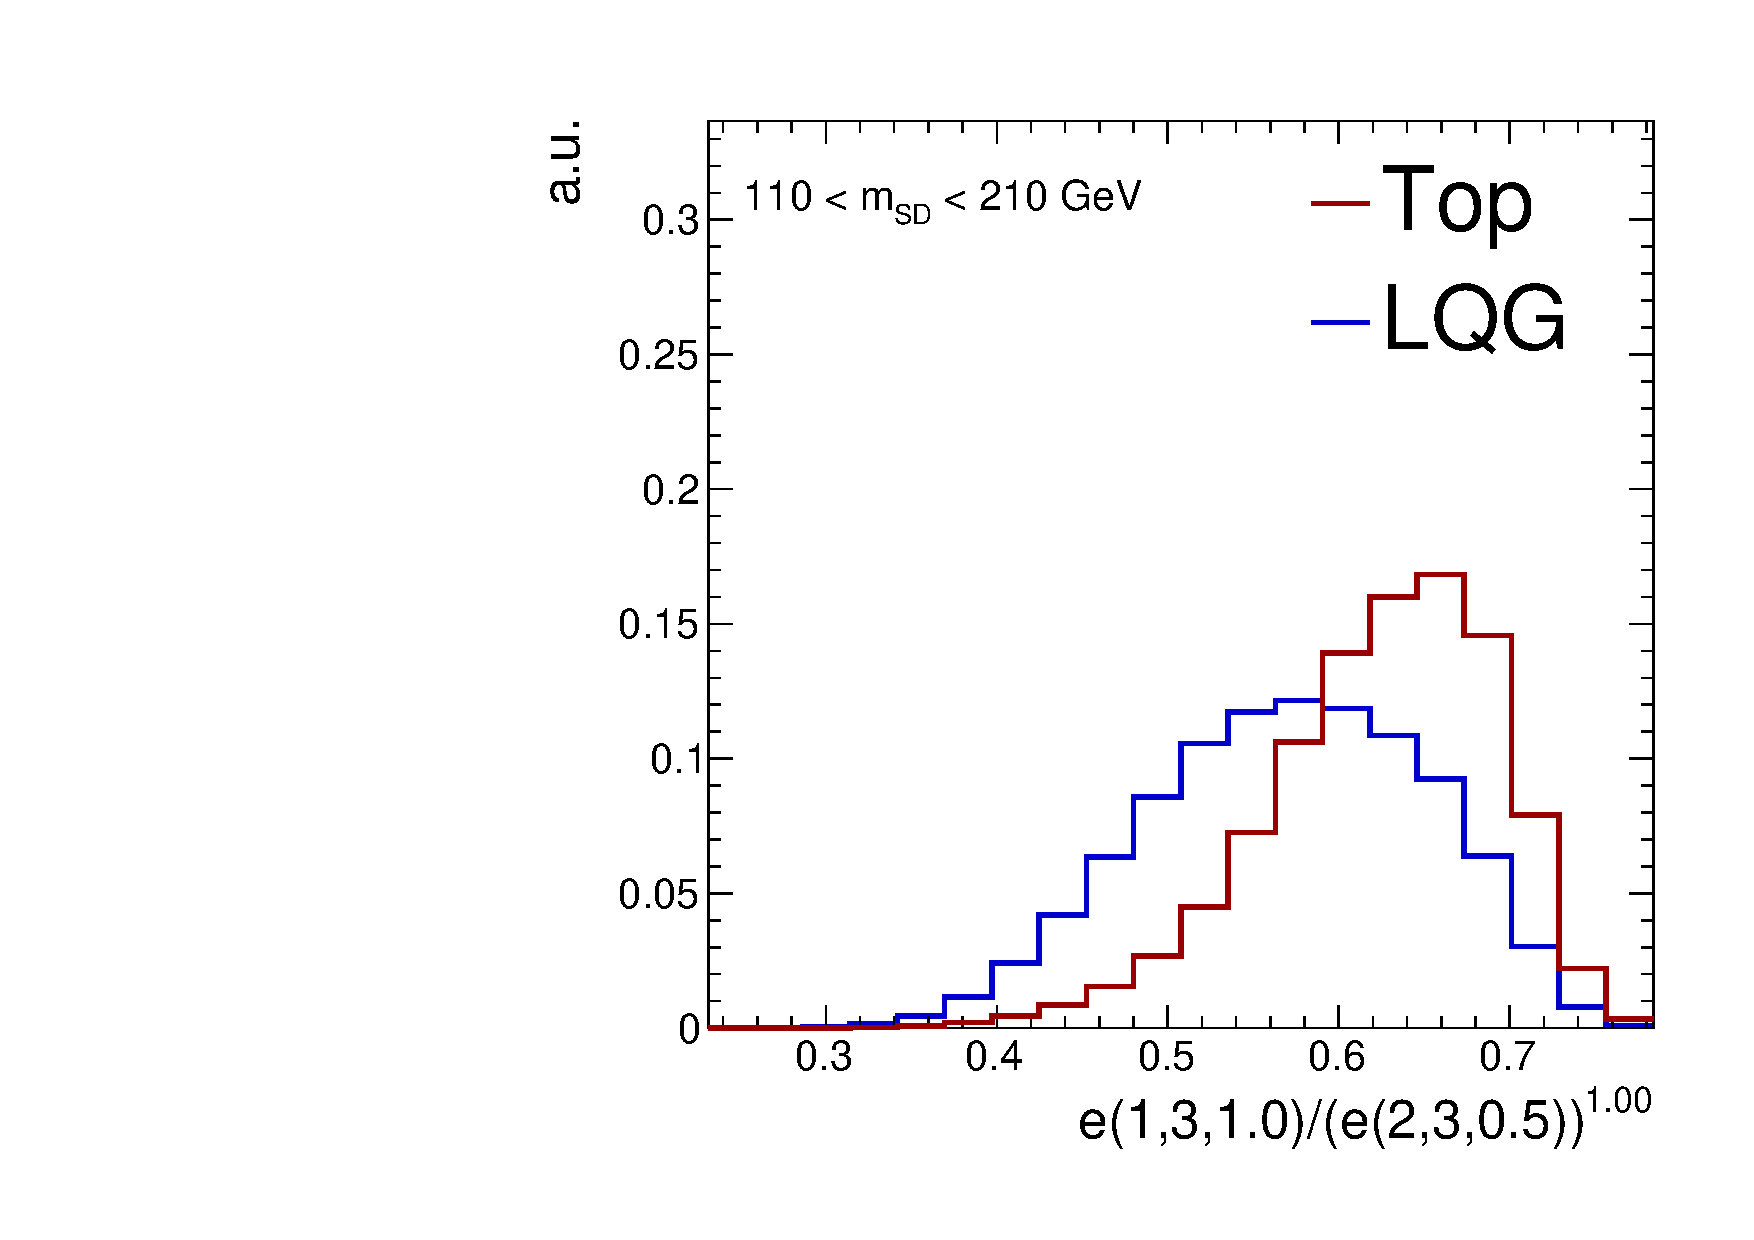
\includegraphics[width=\textwidth]{figures/toptagging/shapes/mass_ratio_13102305.pdf}
        \end{subfigure}
        \begin{subfigure}[t]{0.32\textwidth}
            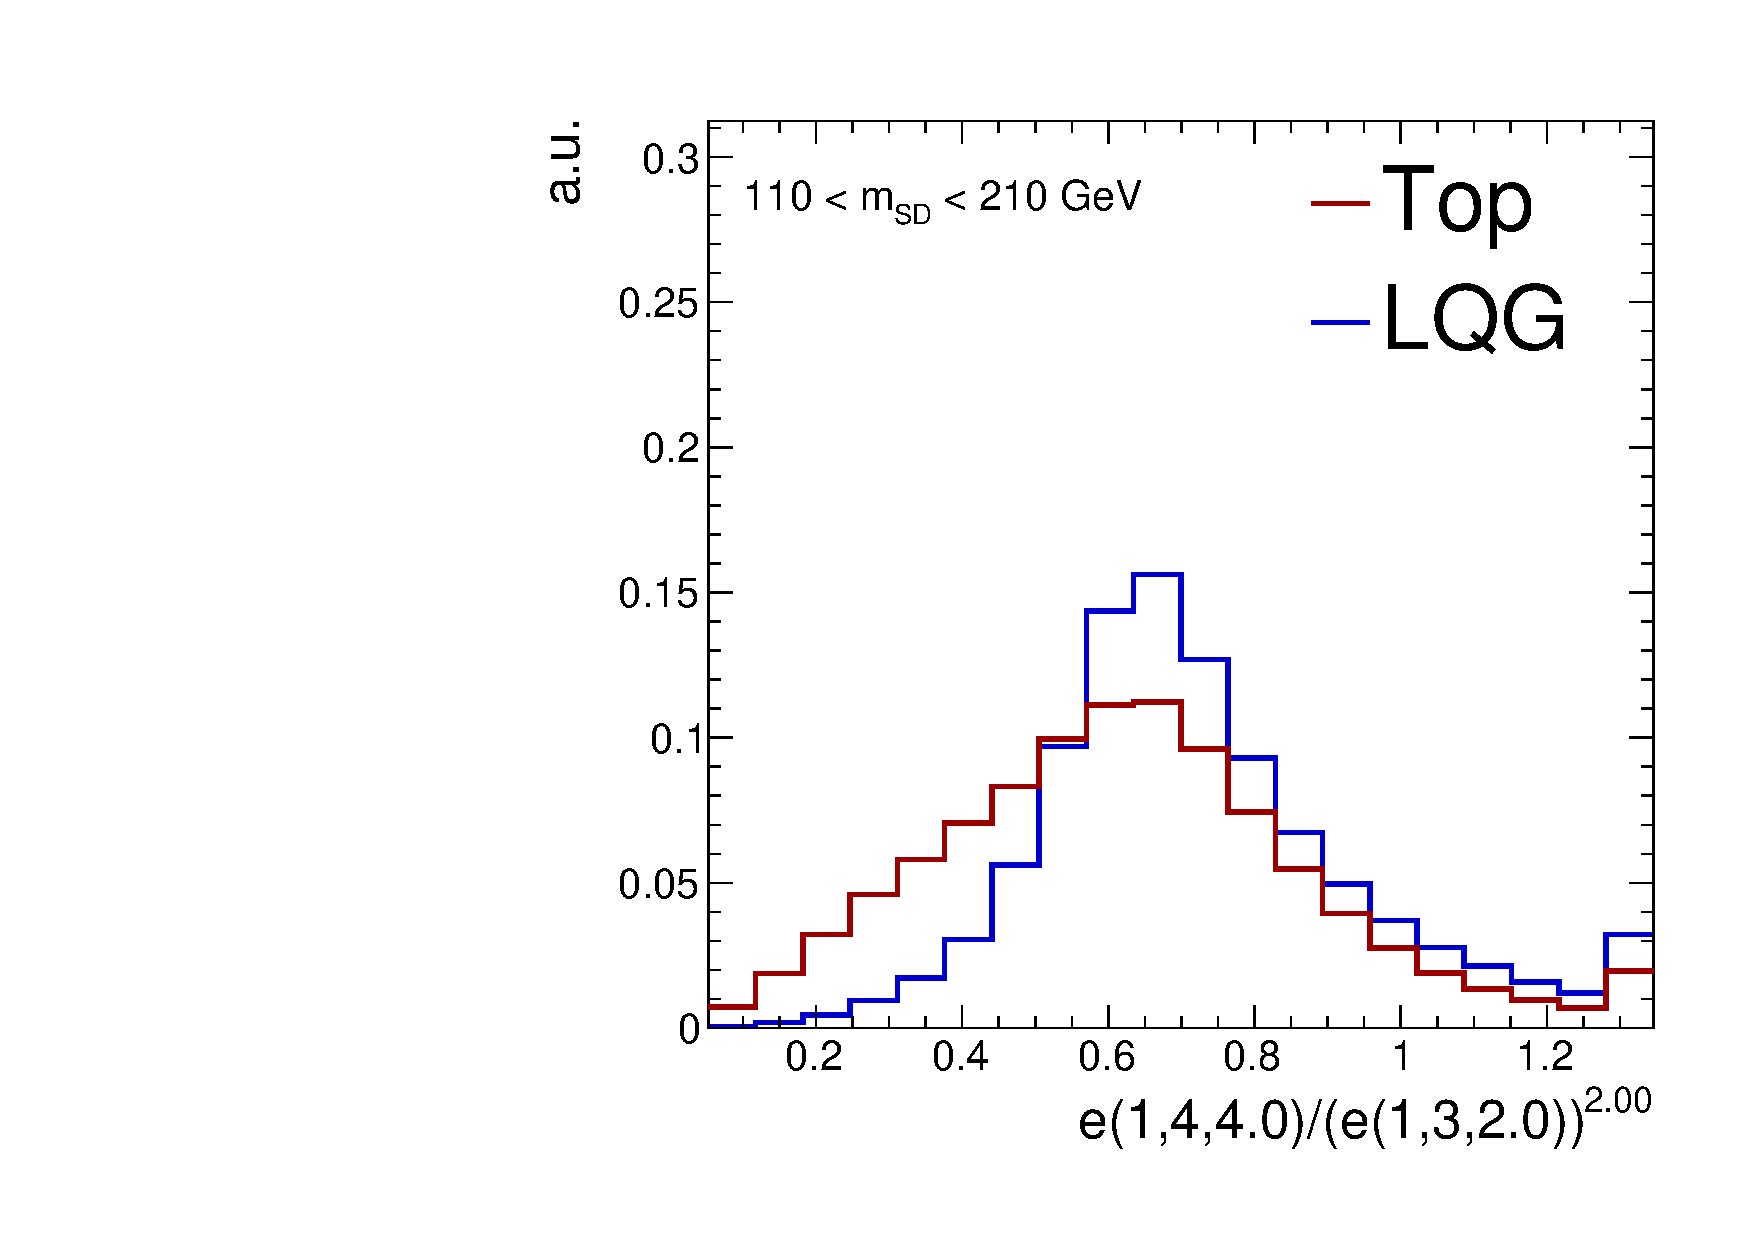
\includegraphics[width=\textwidth]{figures/toptagging/shapes/mass_ratio_14401320.pdf}
        \end{subfigure}
        \caption{Examples of non-trivial ECF ratios other than $N_3$ that separate top and LQG jet distributions.}
        \label{fig:jets:ecfrs}
    \end{center}
\end{figure}


\subsection{A combined tagger}
\label{sec:jets:bdt}

In principle, we have constructed an infinitely large space of substructure observables.
In practice, we only consider a finite sampling of ECF parameters:
\begin{gather}
    N \in \{1,2,3,4\} \nonumber \\ 
    o \in \{1,2,3\} \nonumber \\ 
    \beta \in \{0.5, 1, 2, 4\}
\end{gather}
This grid results in $\sim900$ $\psi$ observables.

To build a single optimal observable out of all the $\{\psi_i\}$s, we will use a boosted decision tree (BDT).
A simplified algorithm to train a single decision tree node $n$ is as follows:
\begin{enumerate}
    \item Choose a $\psi_j$, either by sampling randomly or selecting the one most optimal for the next step.
    \item Based on the training data fed to the node, select a decision boundary $d_n$ to optimize a loss function. For example, one can use the cross-entropy loss:
        \begin{gather}
            \ell(X,y;j,d_n) =  -\hat\pi_B\ln\hat\pi_B -\hat\pi_S\ln\hat\pi_S \text{, where } 
            \hat\pi_c = \hat P(y=c | \psi_j < d_n) 
        \end{gather}
\end{enumerate}
A tree is built iteratively:
\begin{enumerate}
    \item Train a node $n$ using the above criteria. 
    \item If a stopping condition is not met (i.e.~maximum number of nodes, minimal improvement in $\ell(n)$), train one node on the samples that pass $n$ and another on the samples that fail.
\end{enumerate}
Figure~\ref{fig:jets:dt} provides a pictorial example of how a decision tree can be built. 

\begin{figure}[]
    \begin{center}
        \begin{subfigure}[t]{0.32\textwidth}
            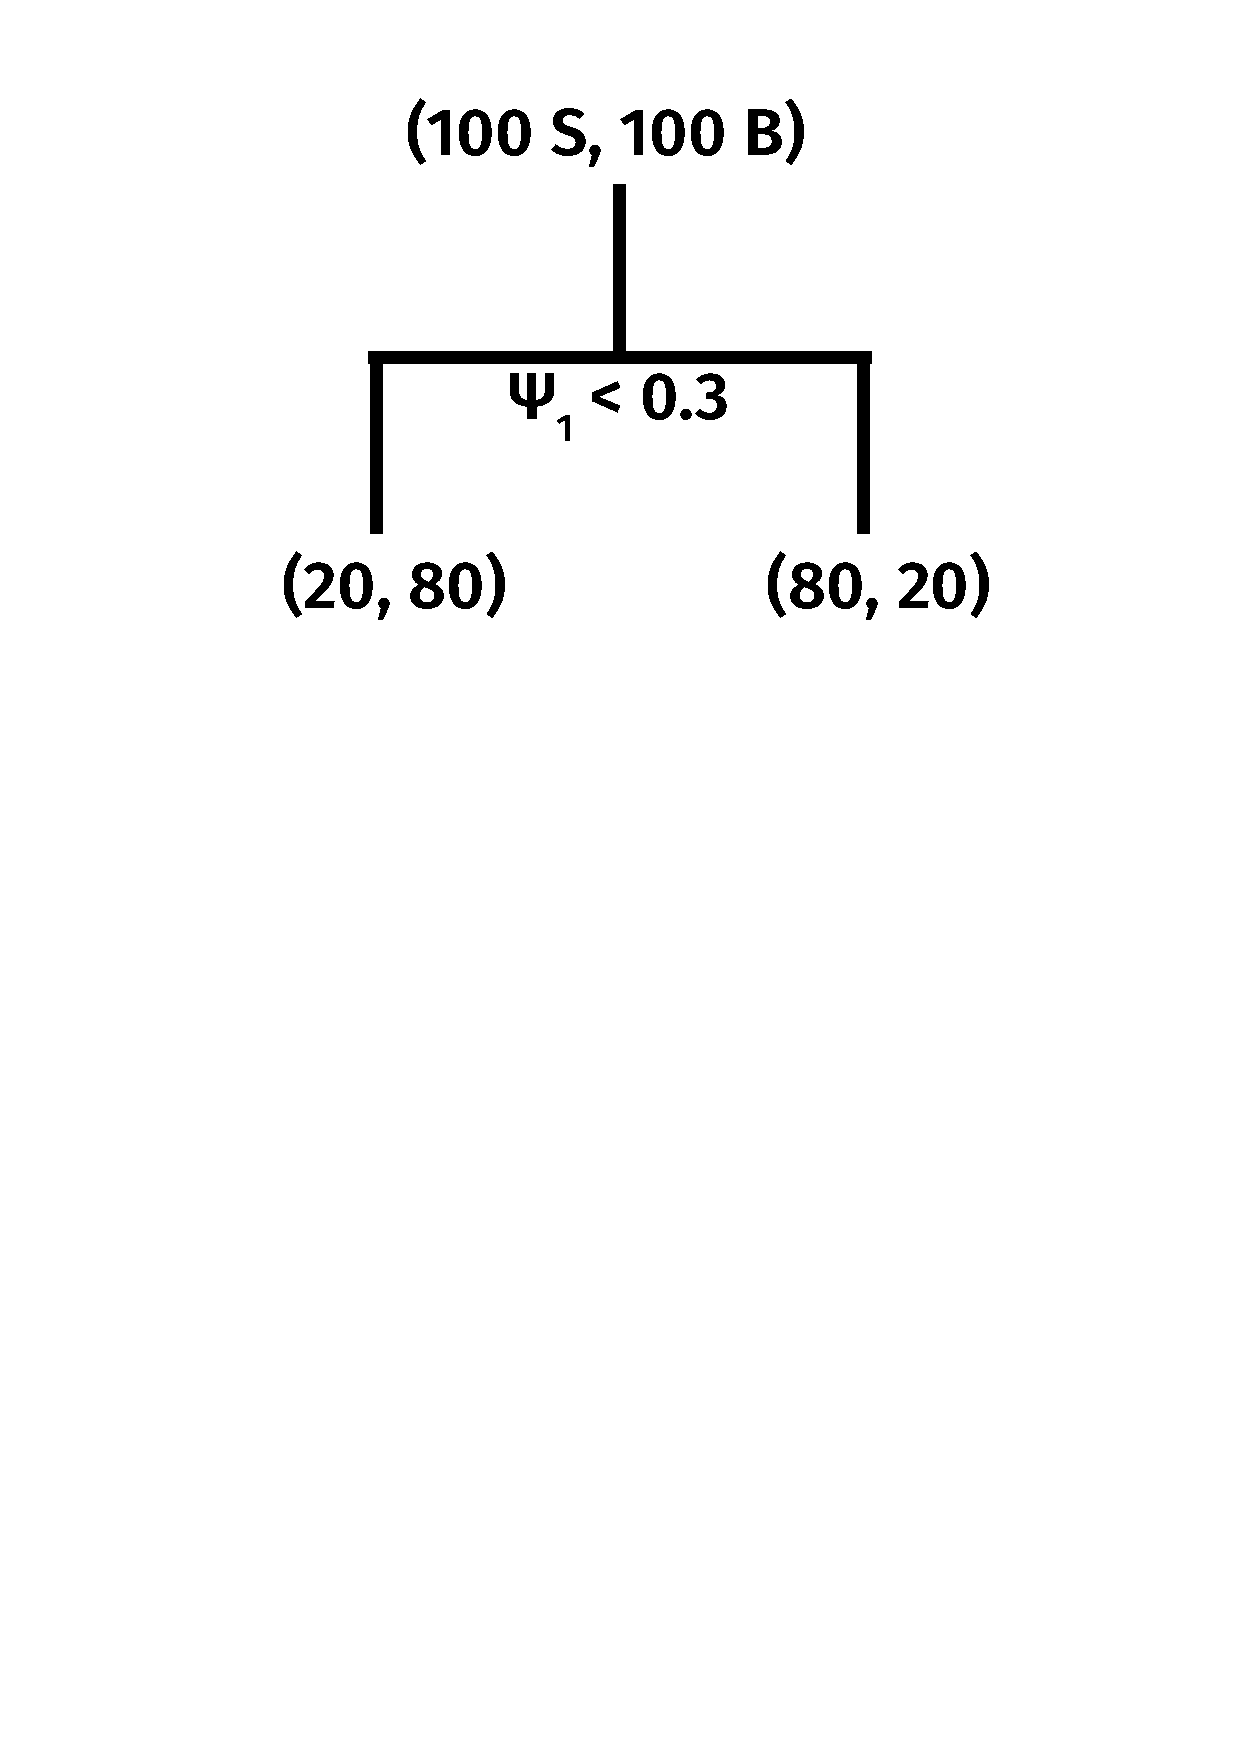
\includegraphics[width=\textwidth]{figures/toptagging/bdt/tree0.pdf}
        \end{subfigure}
        \begin{subfigure}[t]{0.32\textwidth}
            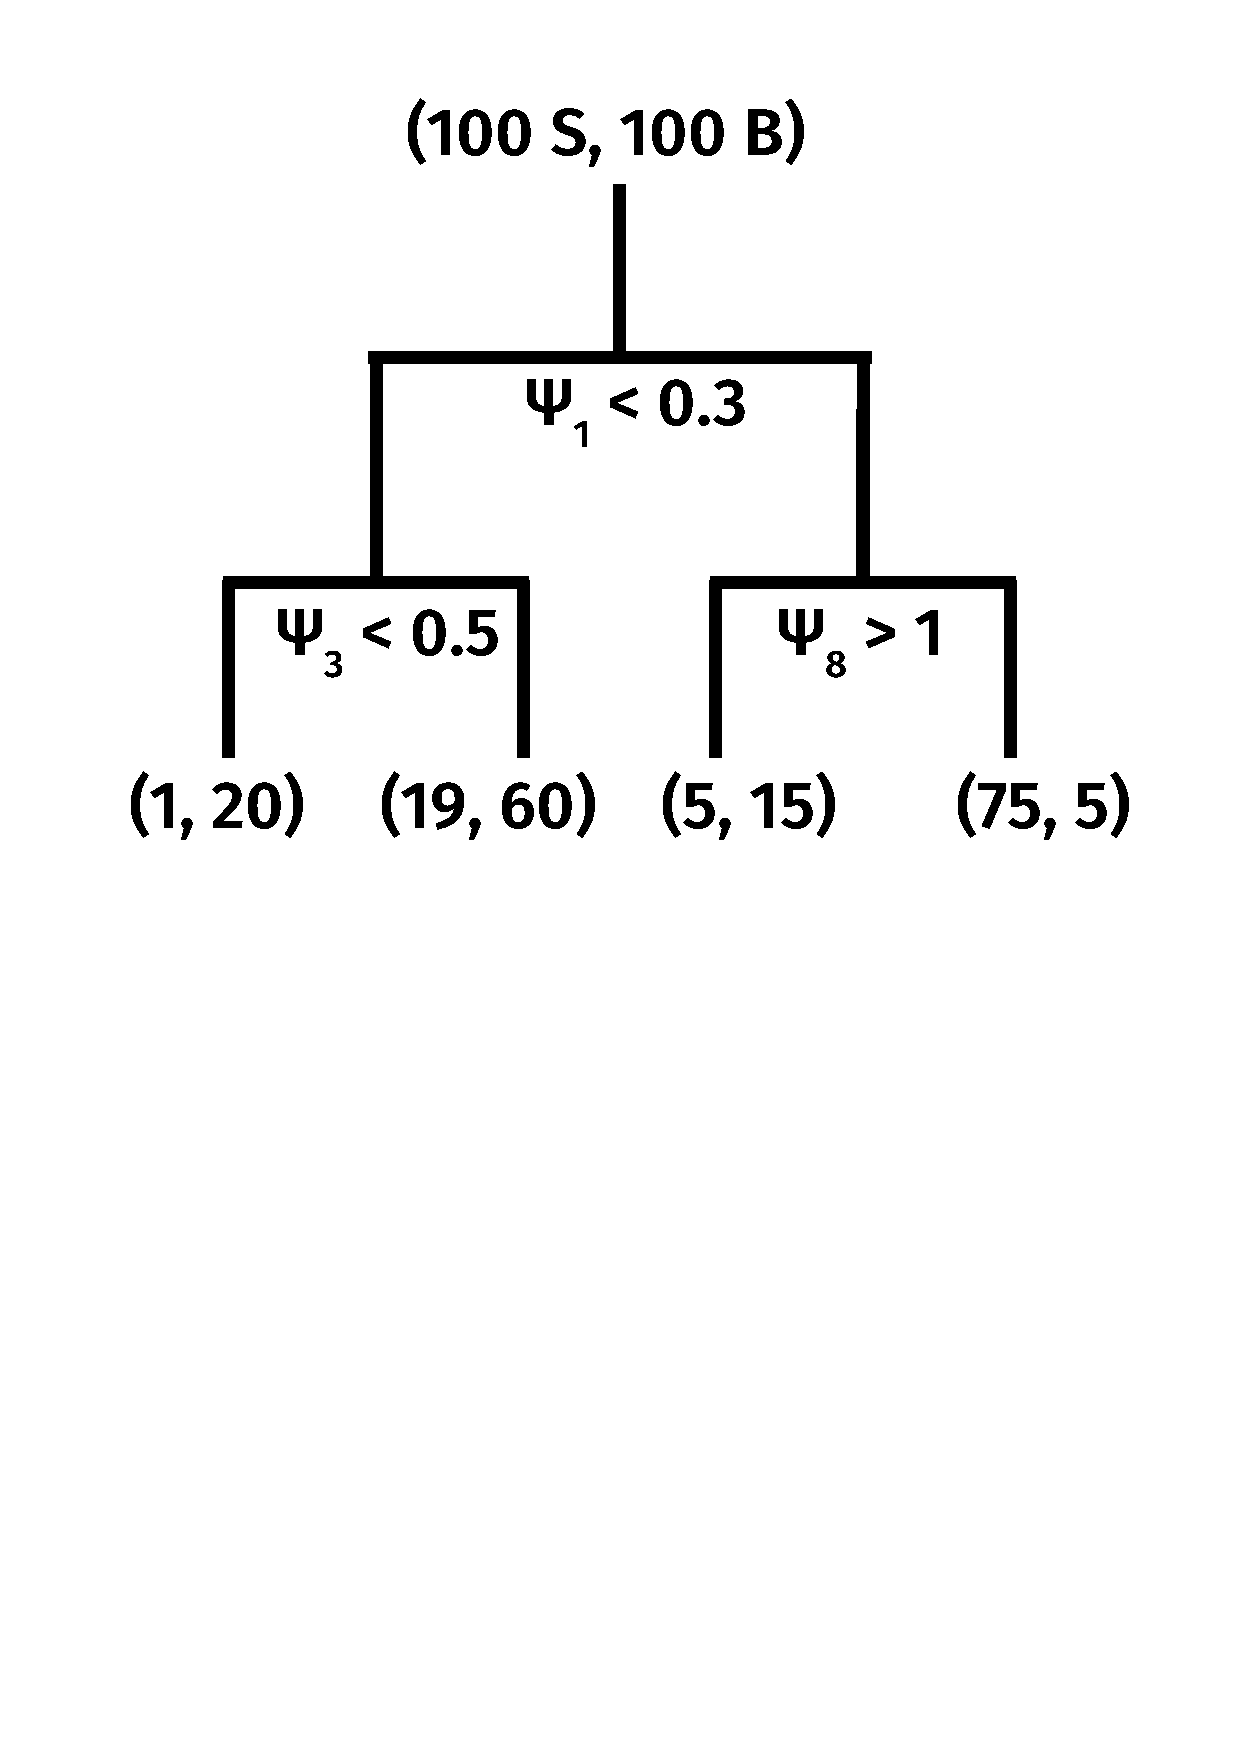
\includegraphics[width=\textwidth]{figures/toptagging/bdt/tree1.pdf}
        \end{subfigure}
        \begin{subfigure}[t]{0.32\textwidth}
            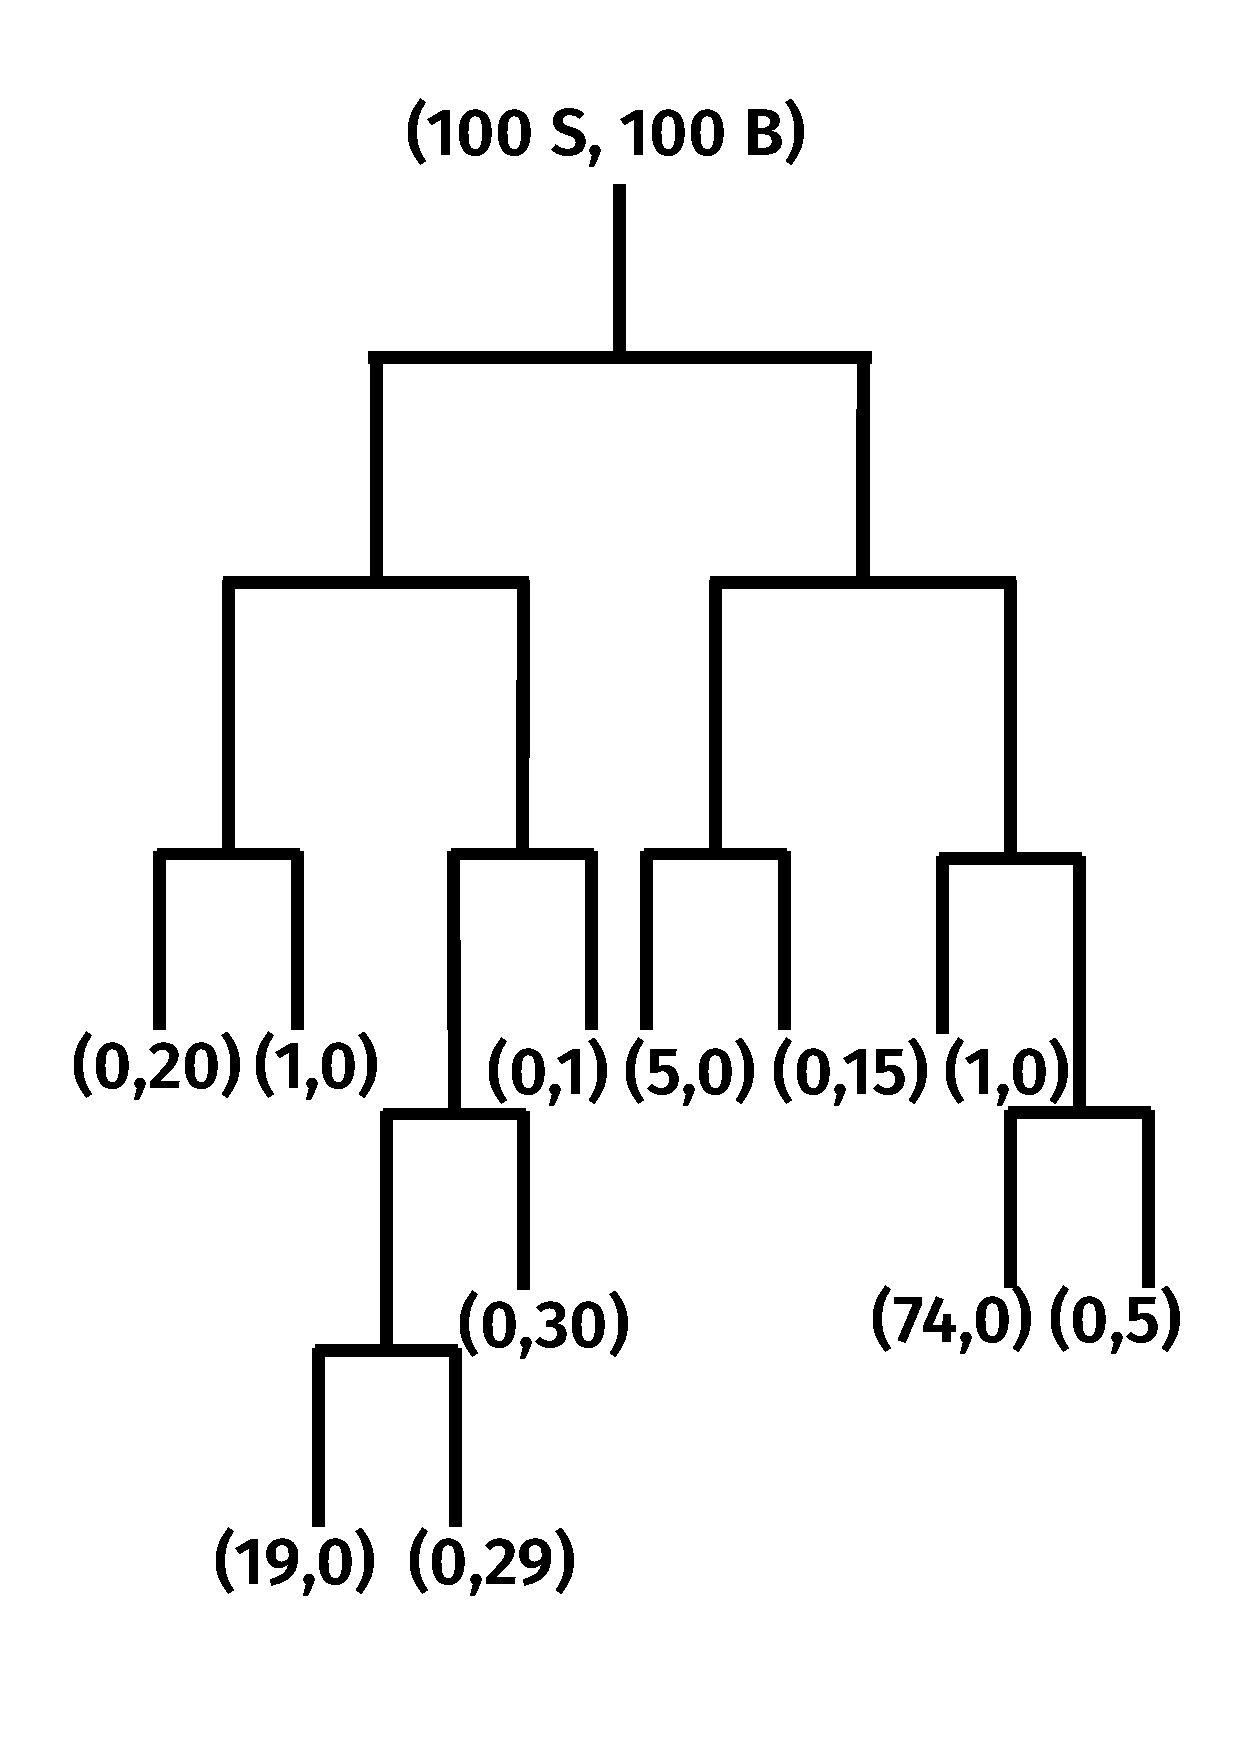
\includegraphics[width=\textwidth]{figures/toptagging/bdt/tree2.pdf}
        \end{subfigure}
        \caption{Steps in greedily training a simple decision tree.}
        \label{fig:jets:dt}
    \end{center}
\end{figure}

While decision trees can very accurately describe training data provided sufficient complexity, they also pathologically overfit the data.
To mitigate this, while retaining descriptive power, a standard method is to \emph{boost} many simple trees.
The simplicity of the tree prevents overfitting, while boosting many trees allows for a complex model.
The result of a BDT is a classifier $f_n(x) = \sum_{i=0}^n \nu^i T_i(x)$, where $\nu\leq 1$ is tunable and each $T_i$ is a decision tree. 
A simplified algorithm to train a BDT is as follows:
\begin{enumerate}
    \item Define a global loss function, e.g.:
        \begin{equation} L(y_i; f_i) = \ln\left(1 + \exp(-y_if_i)\right)\end{equation}
    \item Train a single tree $T_0$ and initialize classifier $f_0 = T_0$
    \item Until some stopping condition (index $m=1,\dots$):
    \begin{enumerate}
      \item[3.1.] Compute the ``residual''
        \begin{equation}r_{mi} = -\nabla_f L(y_i; f) |_{f=f_{m-1}(\bm\psi_i)}\end{equation}
        \begin{equation}L = (y-f_m(\bm\psi))^2 \Rightarrow r_m = y - f_m(\bm\psi) \end{equation}
      \item[3.2.] Fit a regression tree $T_m$ to predict $r_{mi}$ as a function of $x_i$:
        \begin{equation}\ell(X,r_m;j,d,\hat{r}) = \sum_{i | \psi_{ji} < d} (r_{mi} - \hat r)^2\end{equation}
      \item[3.3.] Update $f_m = f_{m-1} + \nu T_m$
    \end{enumerate}
\end{enumerate}

While we would like to train a BDT on the entire space of $\{\psi\}$, there are two issues to be solved: poorly modeled ratios and a large feature space.
Firstly, not every ECF ratio is well-simulated by our MC (Figure~\ref{fig:jets:datamc_ratios}).
More systematically, we can compute the CDFs of each $\psi$ and define a score: 
\begin{equation}
    -\log_{10} \mathrm{KS}(F(\psi_i | \mathrm{data}), F(\psi_i | \mathrm{MC})) = -\log_{10} \max \left|F(\psi_i | \mathrm{data}) - F(\psi_i | \mathrm{MC})\right|
\end{equation}
where $F$ represents the CDF and $\mathrm{KS}$ denotes the Kolmogorov-Smirnov metric on probability distributions.
The score is close to 0 for poorly-simulated distributions.
Figure~\ref{fig:jets:ks} parameterizes this as a function of $N/M$ (ratio of the number of particles) and $a\alpha/b\beta$ (ratio of the angular powers) and shows an interesting structure.
It is found that $3/2$ and $4/2$ ratios are uniformly poorly modeled, as are ratios with large $a\alpha/b\beta$. 
While this structure is interesting and suggestive, we do not yet understand its origin, and therefore do not use this parameterization to select ECF ratios.
Instead, we simply reject any ECF ratio for which $-\log_{10}\mathrm{KS} < 1$. 

\begin{figure}[]
    \begin{center}
        \begin{subfigure}[t]{0.32\textwidth}
            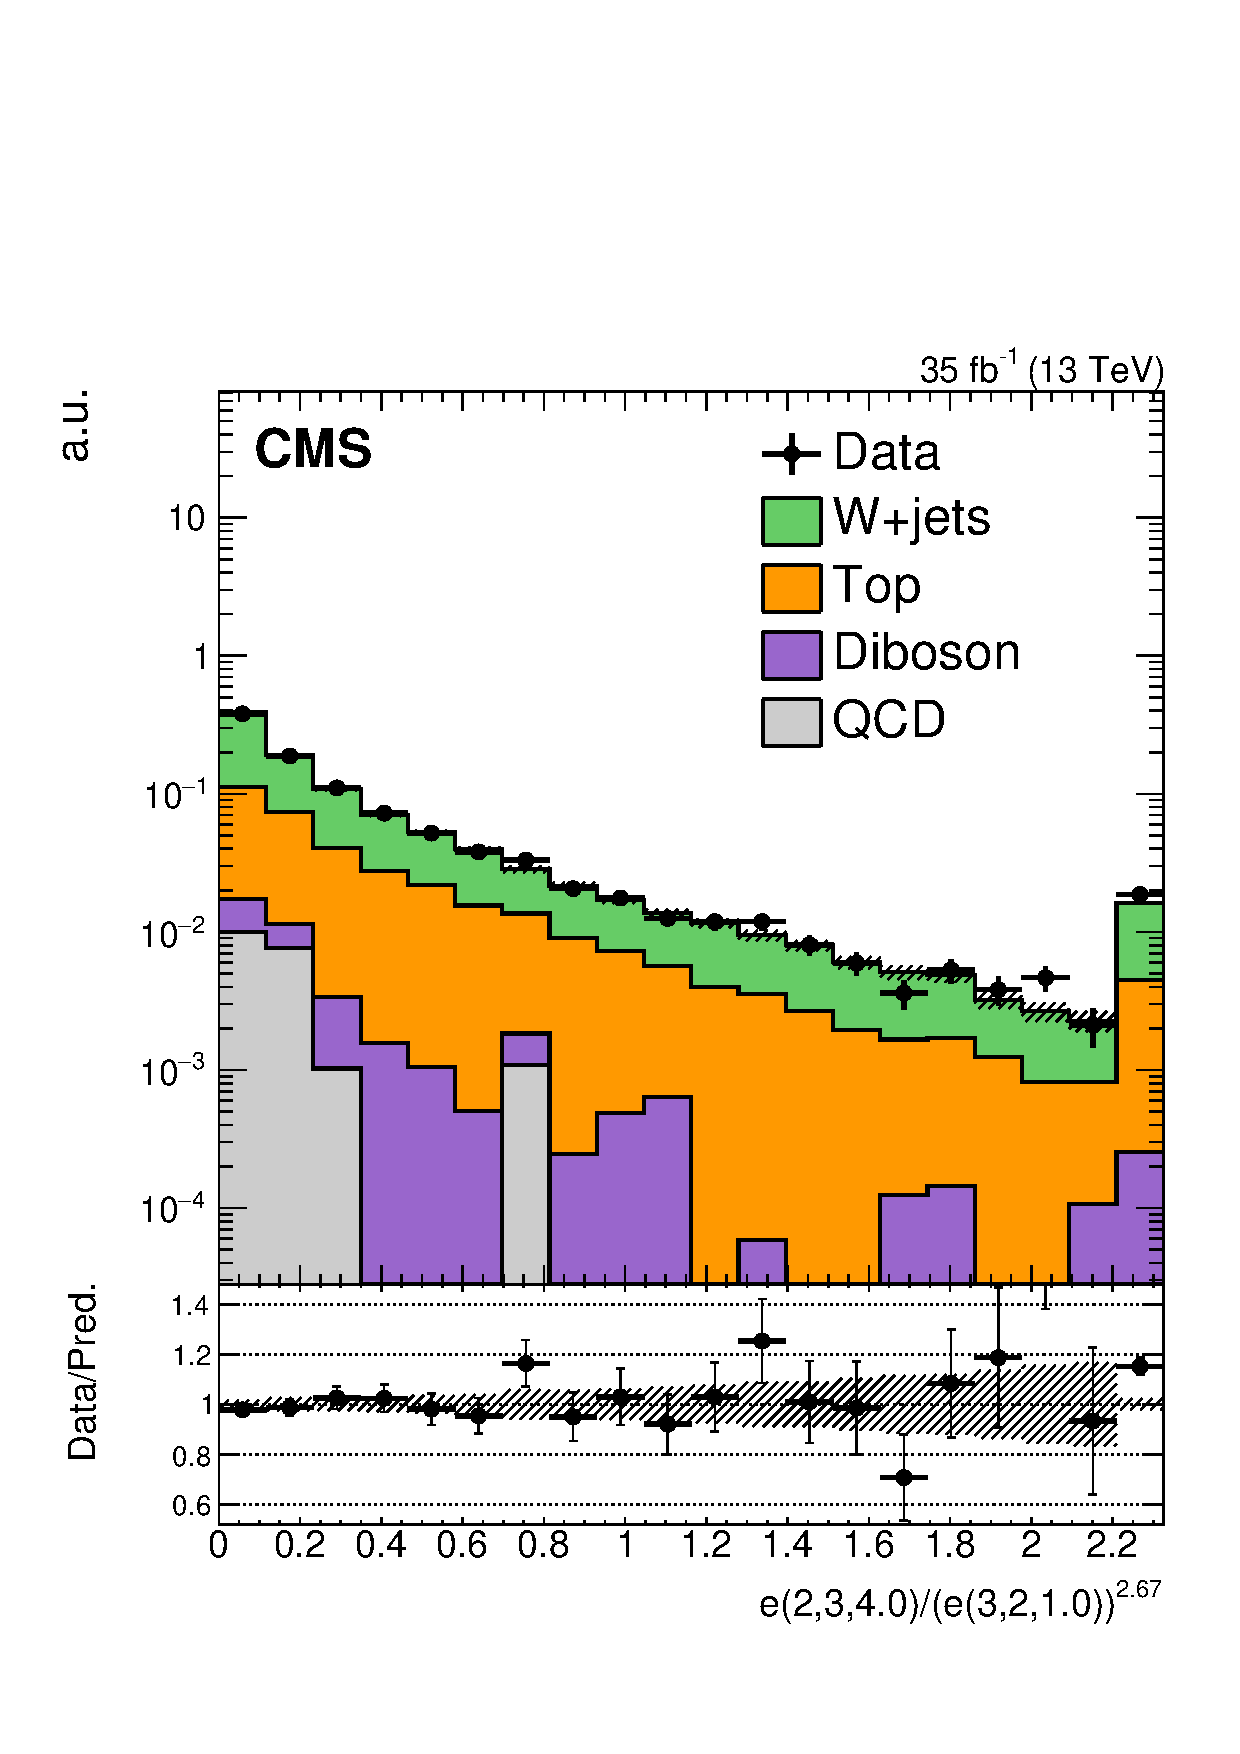
\includegraphics[width=\textwidth]{figures/toptagging/datamc/singlemuonw_ratio_23403210_logy.pdf}
        \end{subfigure}
        \begin{subfigure}[t]{0.32\textwidth}
            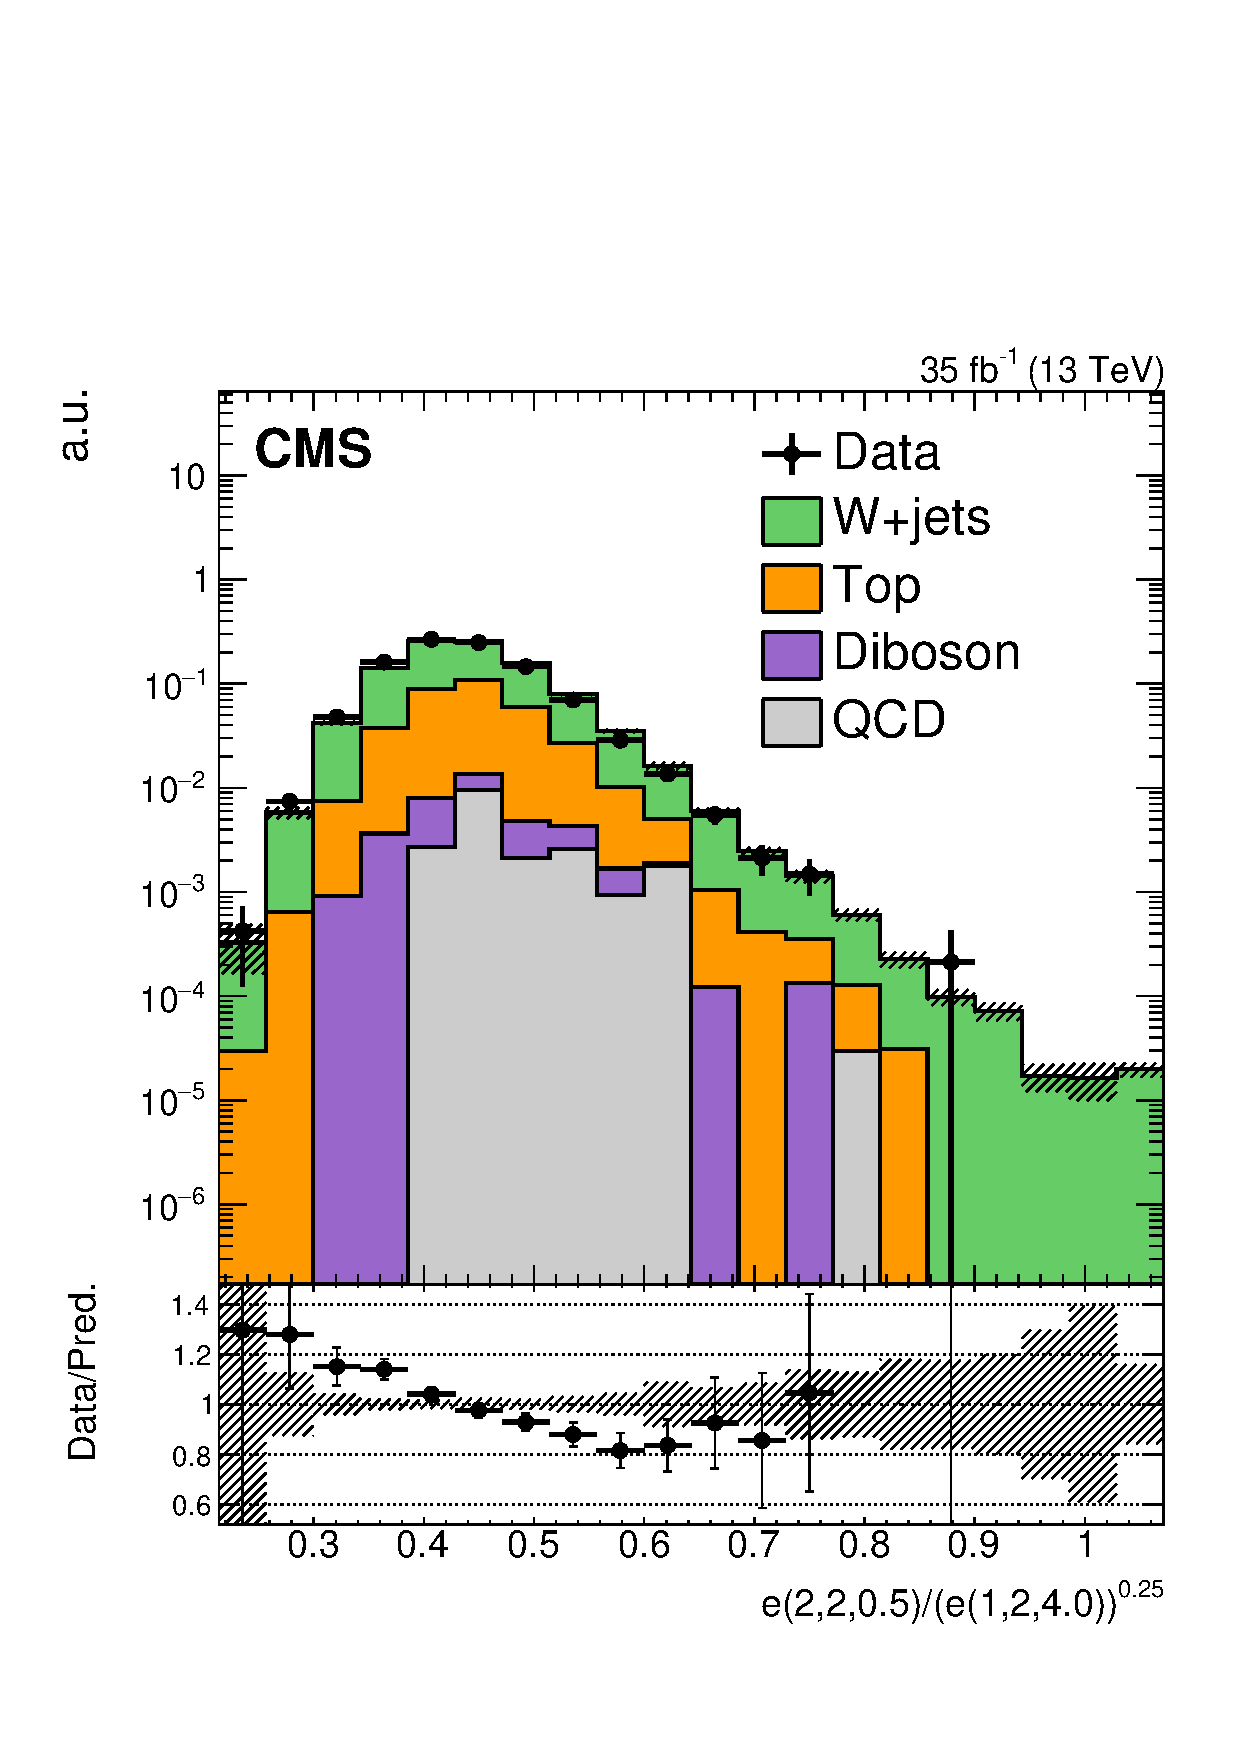
\includegraphics[width=\textwidth]{figures/toptagging/datamc/singlemuonw_ratio_22051240_logy.pdf}
        \end{subfigure}
        \caption{Two different ECF ratios in a $W$+jets selection, heavily enriched in LQG jets.
                 One is fairly well-modeled, while the other is not. }
        \label{fig:jets:datamc_ratios}
    \end{center}
\end{figure}

\begin{figure}[]
    \begin{center}
        \begin{subfigure}[t]{0.4\textwidth}
            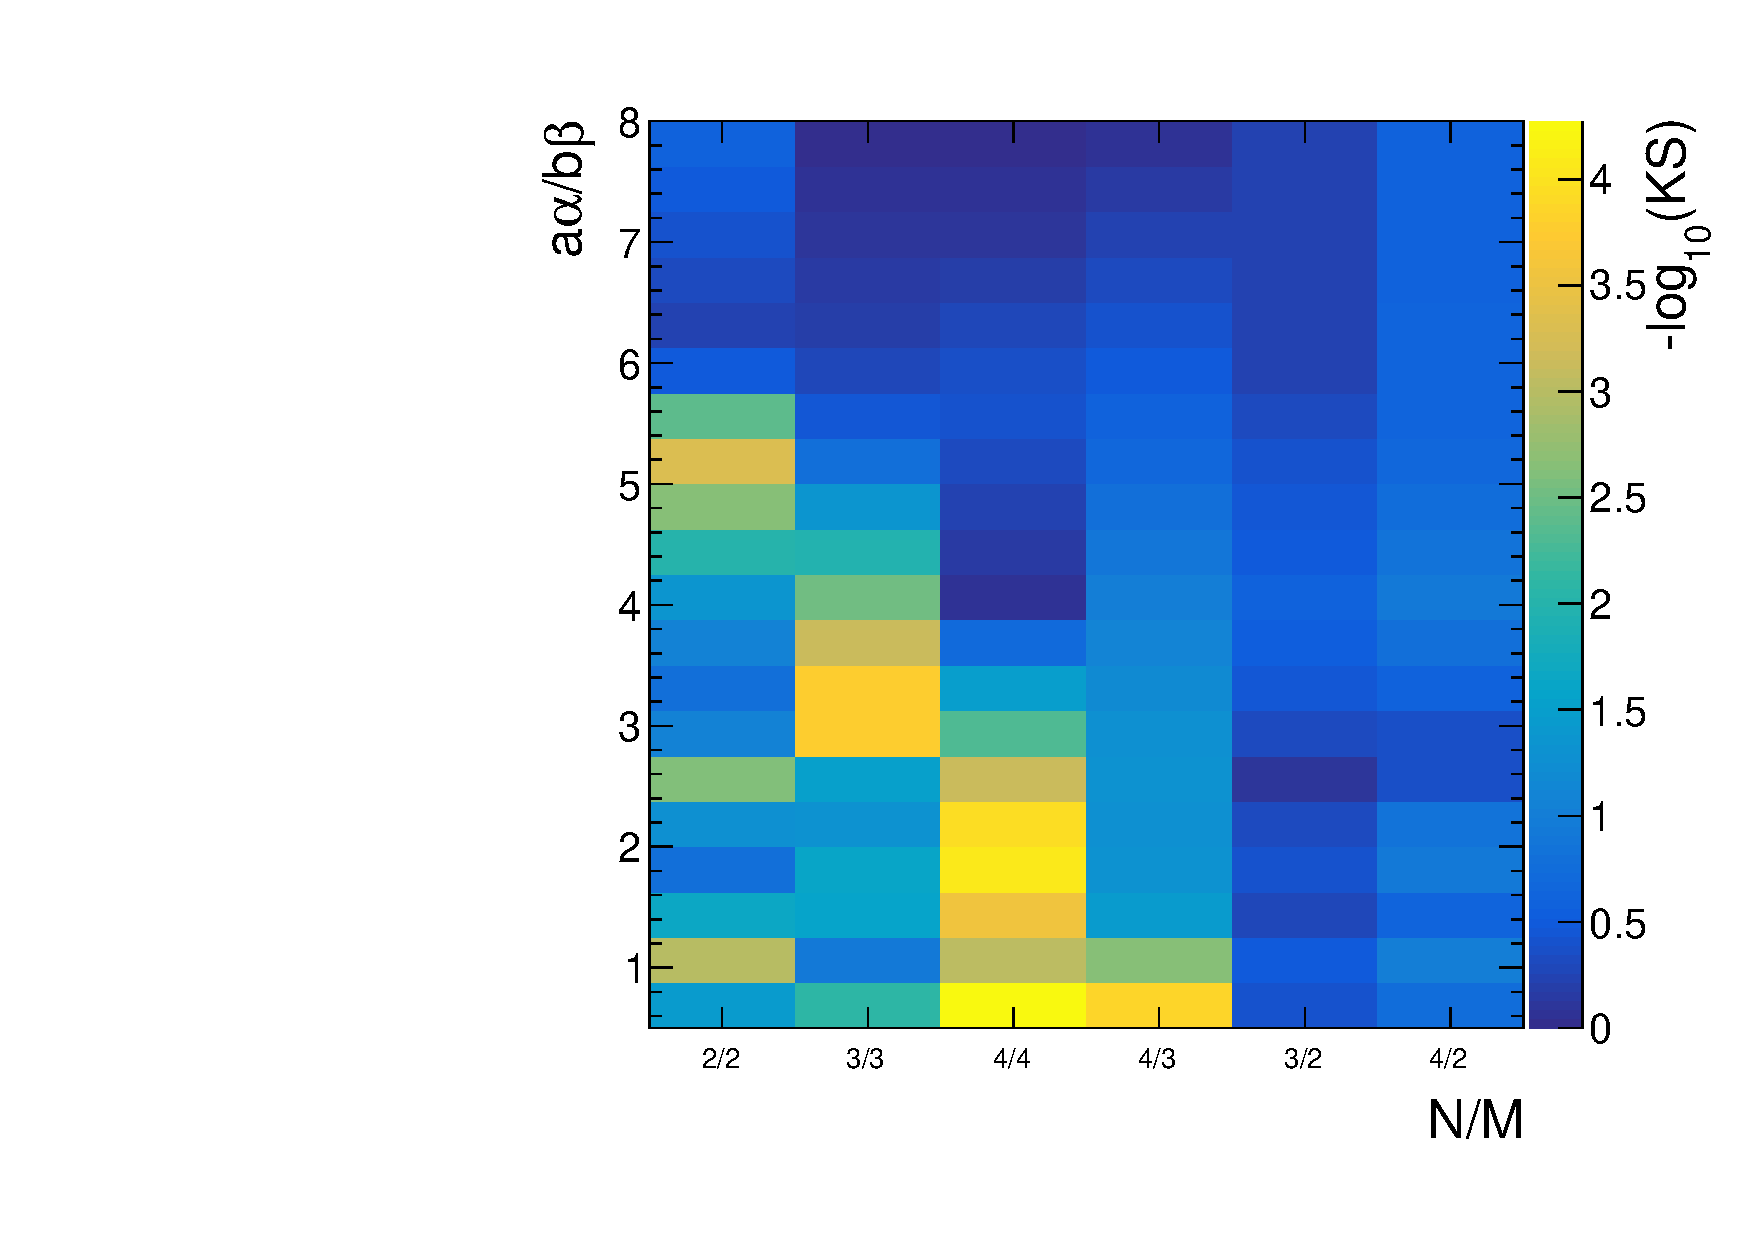
\includegraphics[width=\textwidth]{figures/toptagging/datamc/scanmnab.pdf}
        \end{subfigure}
        \caption{The $-\log_{10}\mathrm{KS}$ metric as a function of $N/M$ and $a\alpha/b\beta$, computed using events enriched in LQG jets. }
        \label{fig:jets:ks}
    \end{center}
\end{figure}

Even after filtering poorly-modeled ratios, we are left with a sampled $\psi$ grid of $\sim 400$ points.
By inspection, many of the $\psi$s are highly correlated or not useful at all.
It is desirable to reduce the size of the feature space, as computing each ECF is somewhat computationally-intensive: an $N$-point ECF on a $p$-particle jet has $\binom{N}{p}$ terms. 
Note that standard pre-processing techniques, like principal component analysis, do not reduce the number of features to be computed. 
While L1 regularization does attempt such a dimensional reduction, it cannot be trivially applied to BDTs. 
Therefore, we introduce a targeted iterative training method to solve this problem:
\begin{enumerate}
    \item Train a BDT with trees $T_1,\dots,T_n$
    \item For each $\psi_i$, define a score:
        \begin{equation}
             s_i = \sum_{m=1}^n \nu^{m-1} \sum_{\text{nodes using $\psi_i$ in $T_m$}} N_\text{samples}(\mathrm{node}) \times \left(\ell(\mathrm{node}) - \ell(\mathrm{parent})\right)^2  
        \end{equation}
    \item Remove (one or more) $\psi_i$ with smallest $s_i$ and repeat until the global loss $L$ worsens significantly
\end{enumerate}
Iterative training is expensive and can require the training of $\mathcal{O}(50)$ BDTs.
It is semi-parallelizable, and the entire process typically takes a few hours.
However, as the inference samples are 1-2 orders of magnitude larger than the training samples, this method reduces the total CPU time needed to run an analysis. 
Figure~\ref{fig:jets:training} shows background acceptance rate at $\epsilon_\mathrm{sig}=0.5$ (a proxy for the global loss) as a function of feature space size. 
For illustrative purposes, we only show the range $[1,50]$.
The inputs for this training are the ECF ratios, as well as $\tau_{32}^\SD$ and $\frec$, which provide additional information.
It is clear that beyond 13-15 features, there is little to be gained by adding additional information.

\begin{figure}[]
    \begin{center}
        \begin{subfigure}[t]{0.4\textwidth}
            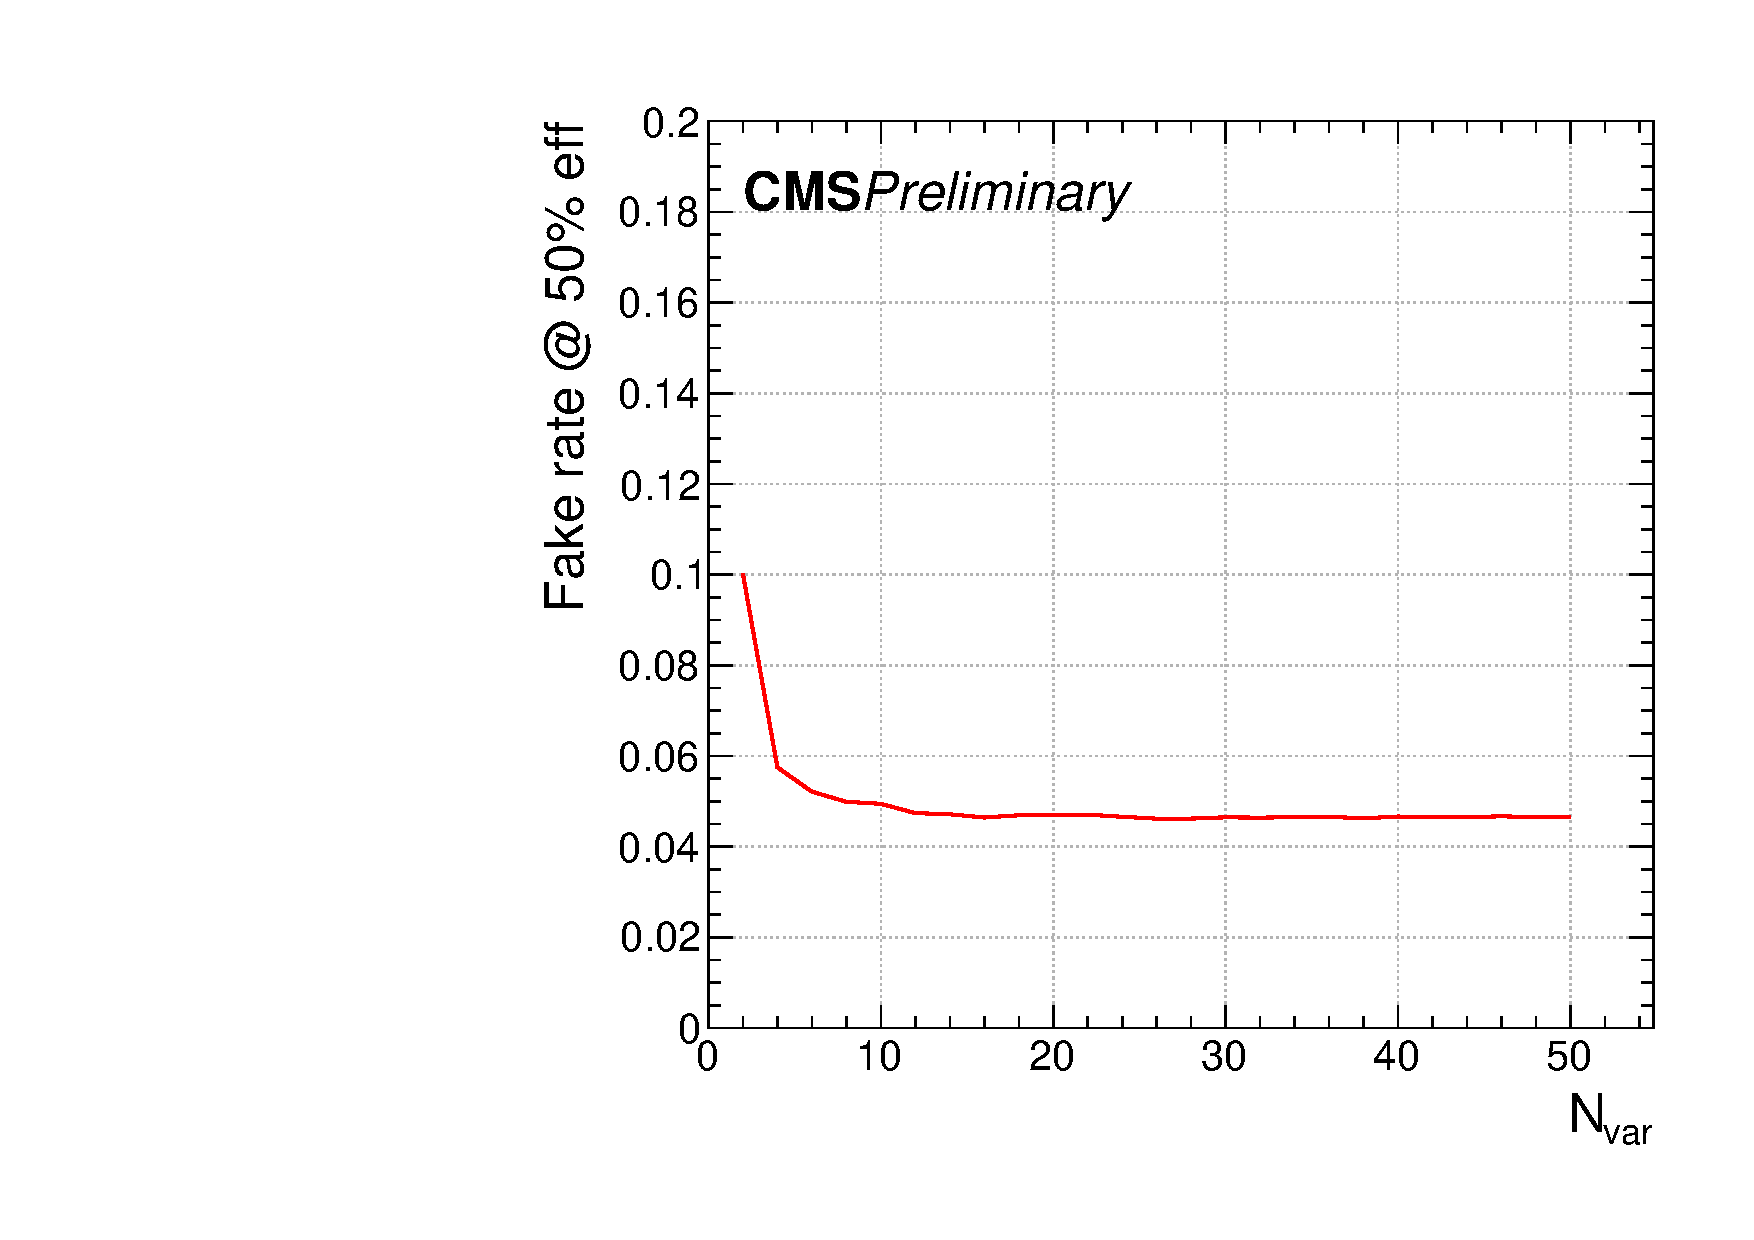
\includegraphics[width=\textwidth]{figures/toptagging/bdt/fakerate_vs_eff50.pdf}
        \end{subfigure}
        \caption{Performance of BDTs as a function of the number features used in the training.}
        \label{fig:jets:training}
    \end{center}
\end{figure}

The features selected by this reduction and classification process are:
\begin{gather}
    \frac{e(1,4,20)}{e(1,3,10)^2},~
    \frac{e(1,4,40)}{e(1,3,20)^2},~
    \frac{e(2,4,05)}{e(1,3,05)^2},~
    \frac{e(2,4,10)}{e(1,3,10)^2},~
    \frac{e(2,4,10)}{e(2,3,05)^2},~
    \frac{e(2,4,20)}{e(1,3,20)^2} \nonumber \\ 
    \frac{e(1,2,20)}{e(1,2,10)^2},~
    \frac{e(1,3,40)}{e(2,3,20)},~
    \frac{e(3,3,10)}{e(1,3,40)^{3/4}},~
    \frac{e(3,3,10)}{e(2,3,20)^{3/4}},~
    \frac{e(3,3,20)}{e(3,3,40)^{1/2}}\nonumber \\ 
    \tau_{32}^\SD,~ \frec 
    \label{eq:jets:features}
\end{gather}
While a number of $N_3$ or other $4/3$ ratios appear in this list, we find a number of $2/2$ and $3/3$ ratios to contribute meaningfully to the classification task as well. 
Figure~\ref{fig:jets:features} shows the distributions of all selected features. 
Figure~\ref{fig:jets:roc} shows the background acceptance as a function of signal efficiency, comparing the final BDT (``Combined BDT``) to several other taggers.
The ``11 ECF`` BDT refers to a BDT trained using only the 11 ECF ratios from Equation~\ref{eq:jets:features}, indicating that $\tau_{32}^\SD$ and $\frec$ are critical to achieving the same performance that can be reached with a much larger ECF ratio set (``50 ECF``).
For comparison, also shown are the efficiency curves for $\tau_{32}^\SD$ and a BDT trained using $\tau_{32}^\SD$ and $\frec$ only.
At fixed signal efficiency $\epsilon_\mathrm{sig} = 0.5$, the combined BDT reduces the background acceptance by 30\% relative to $\tau_{32}^\SD$, the standard top ID criterion at the LHC prior to this study. 

\begin{figure}[]
    \begin{center}
        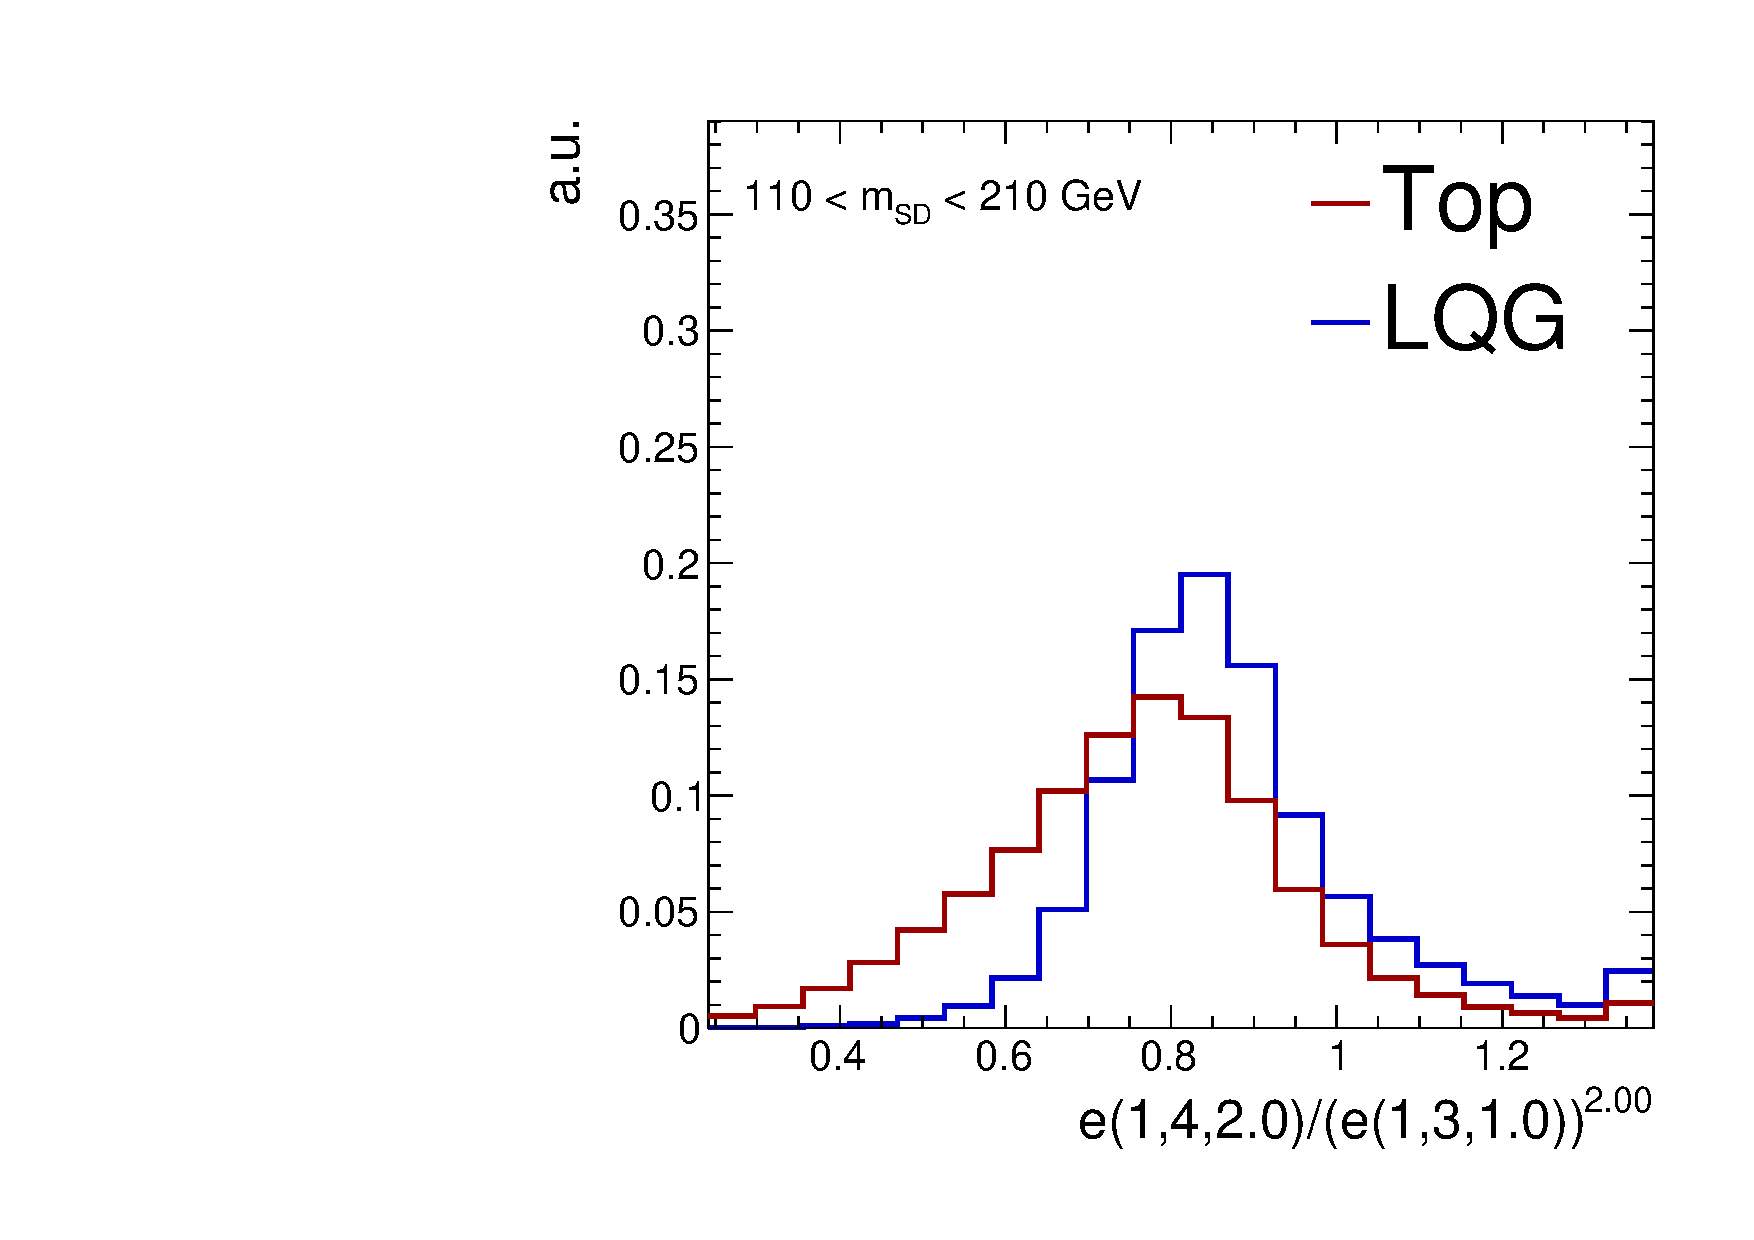
\includegraphics[width=0.24\textwidth]{figures/toptagging/shapes/mass_ratio_14201310.pdf}
        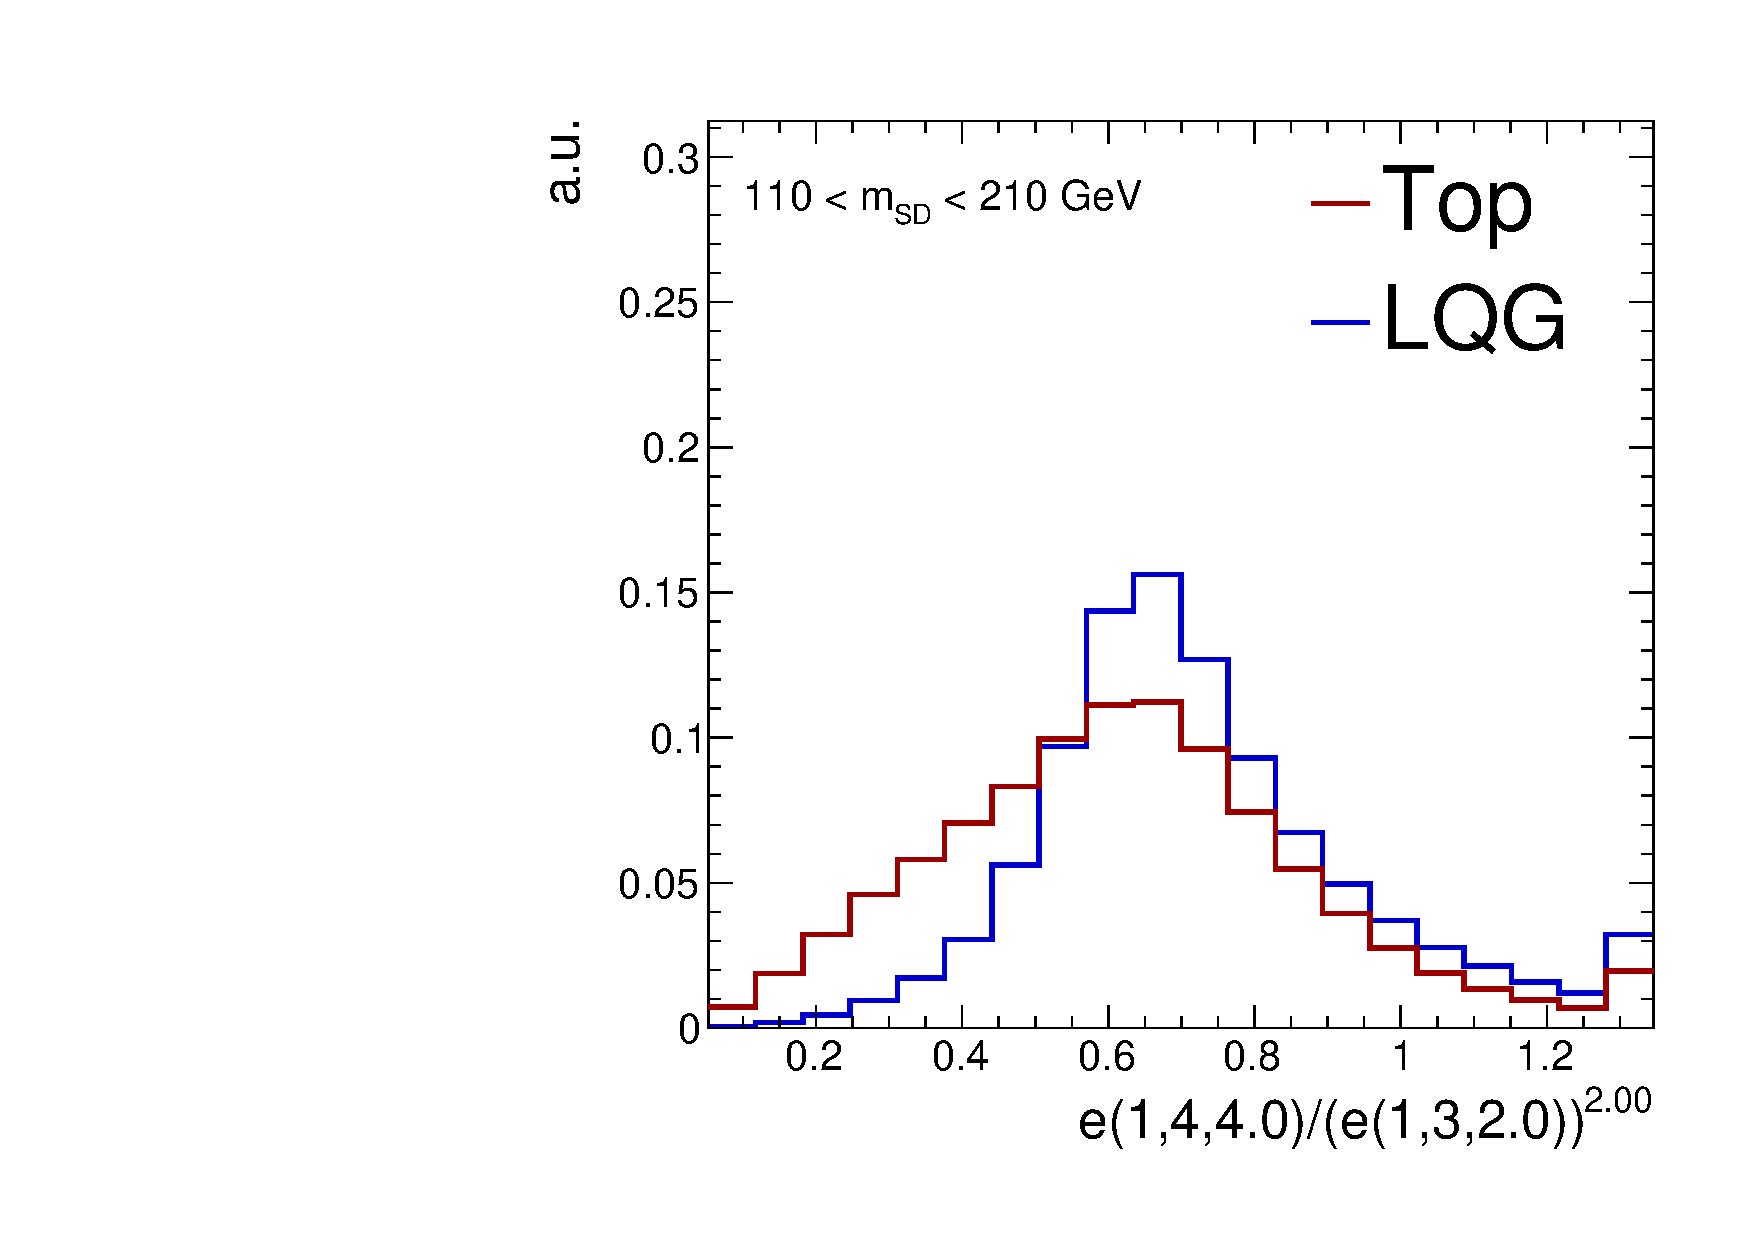
\includegraphics[width=0.24\textwidth]{figures/toptagging/shapes/mass_ratio_14401320.pdf}
        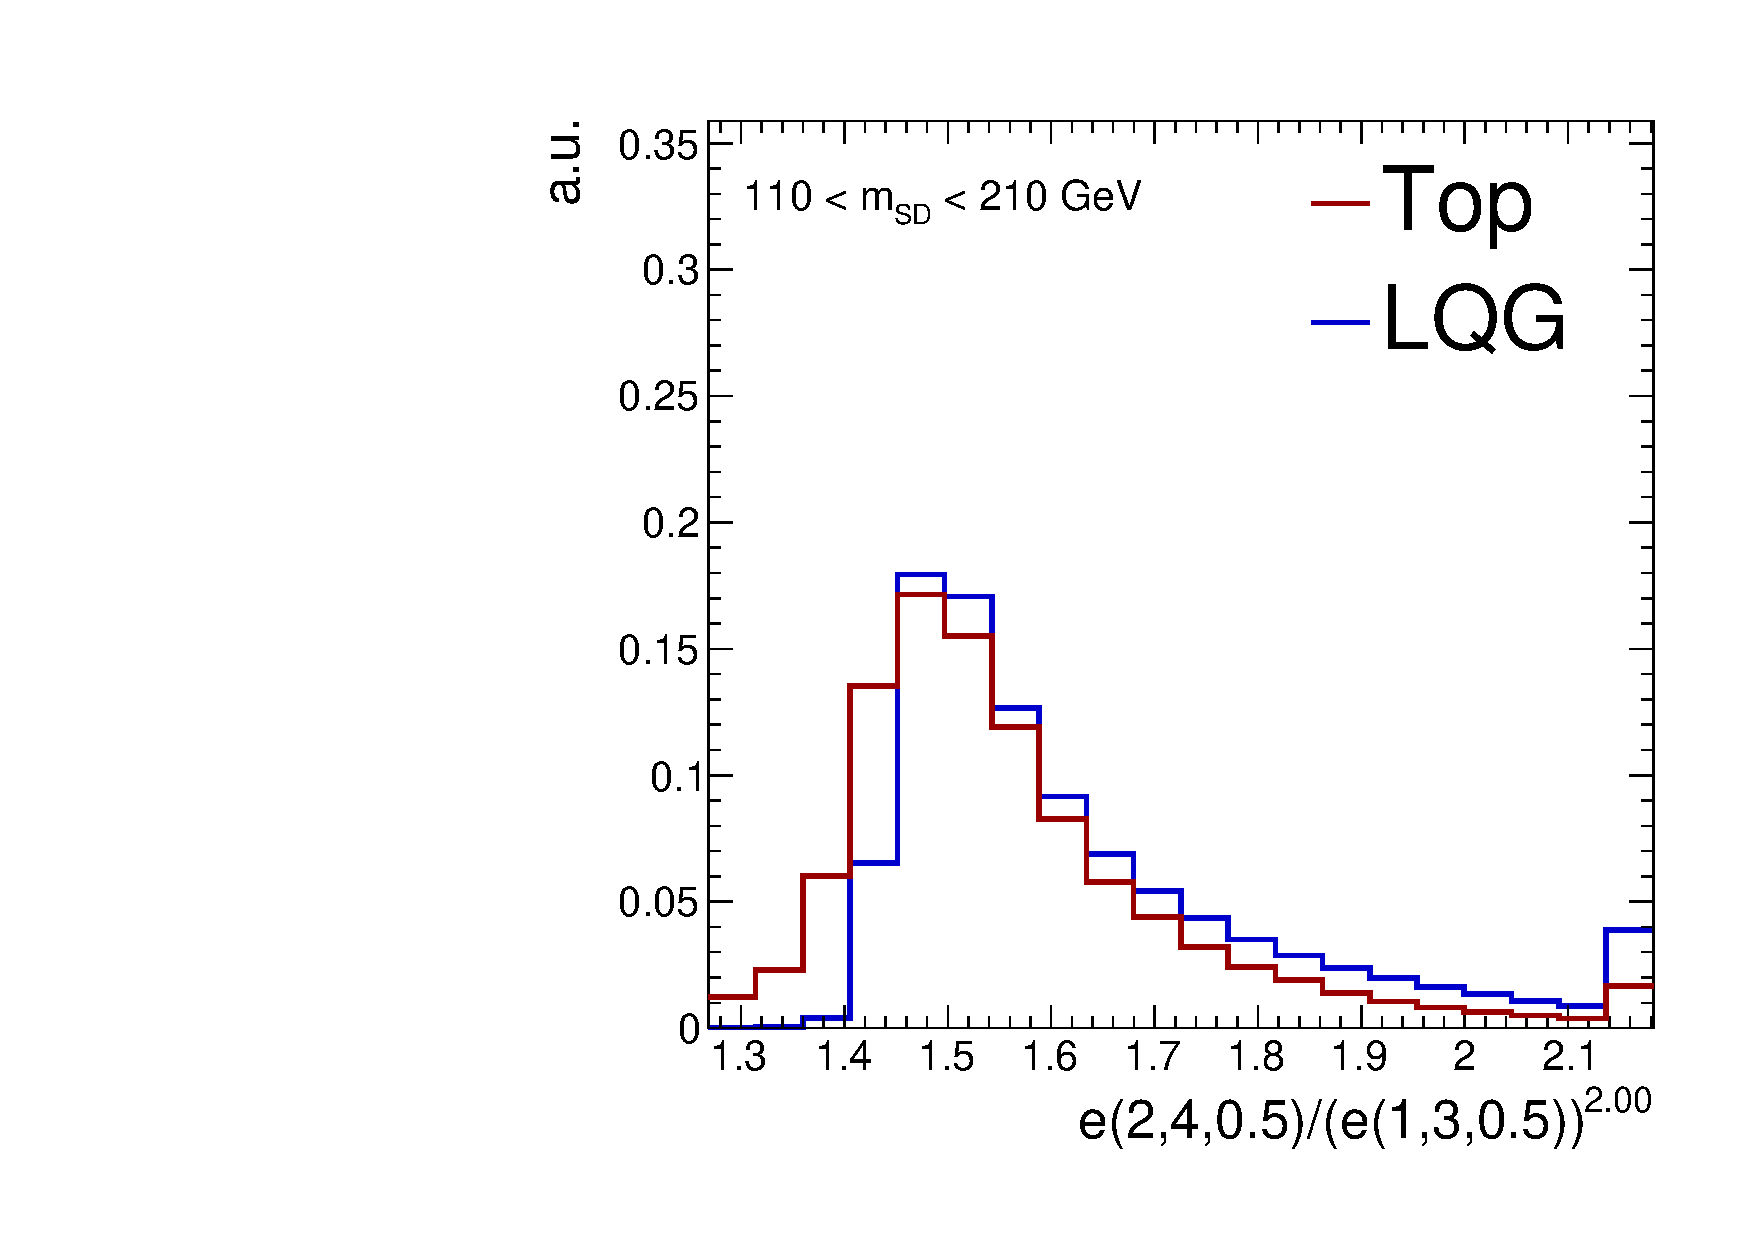
\includegraphics[width=0.24\textwidth]{figures/toptagging/shapes/mass_ratio_24051305.pdf}
        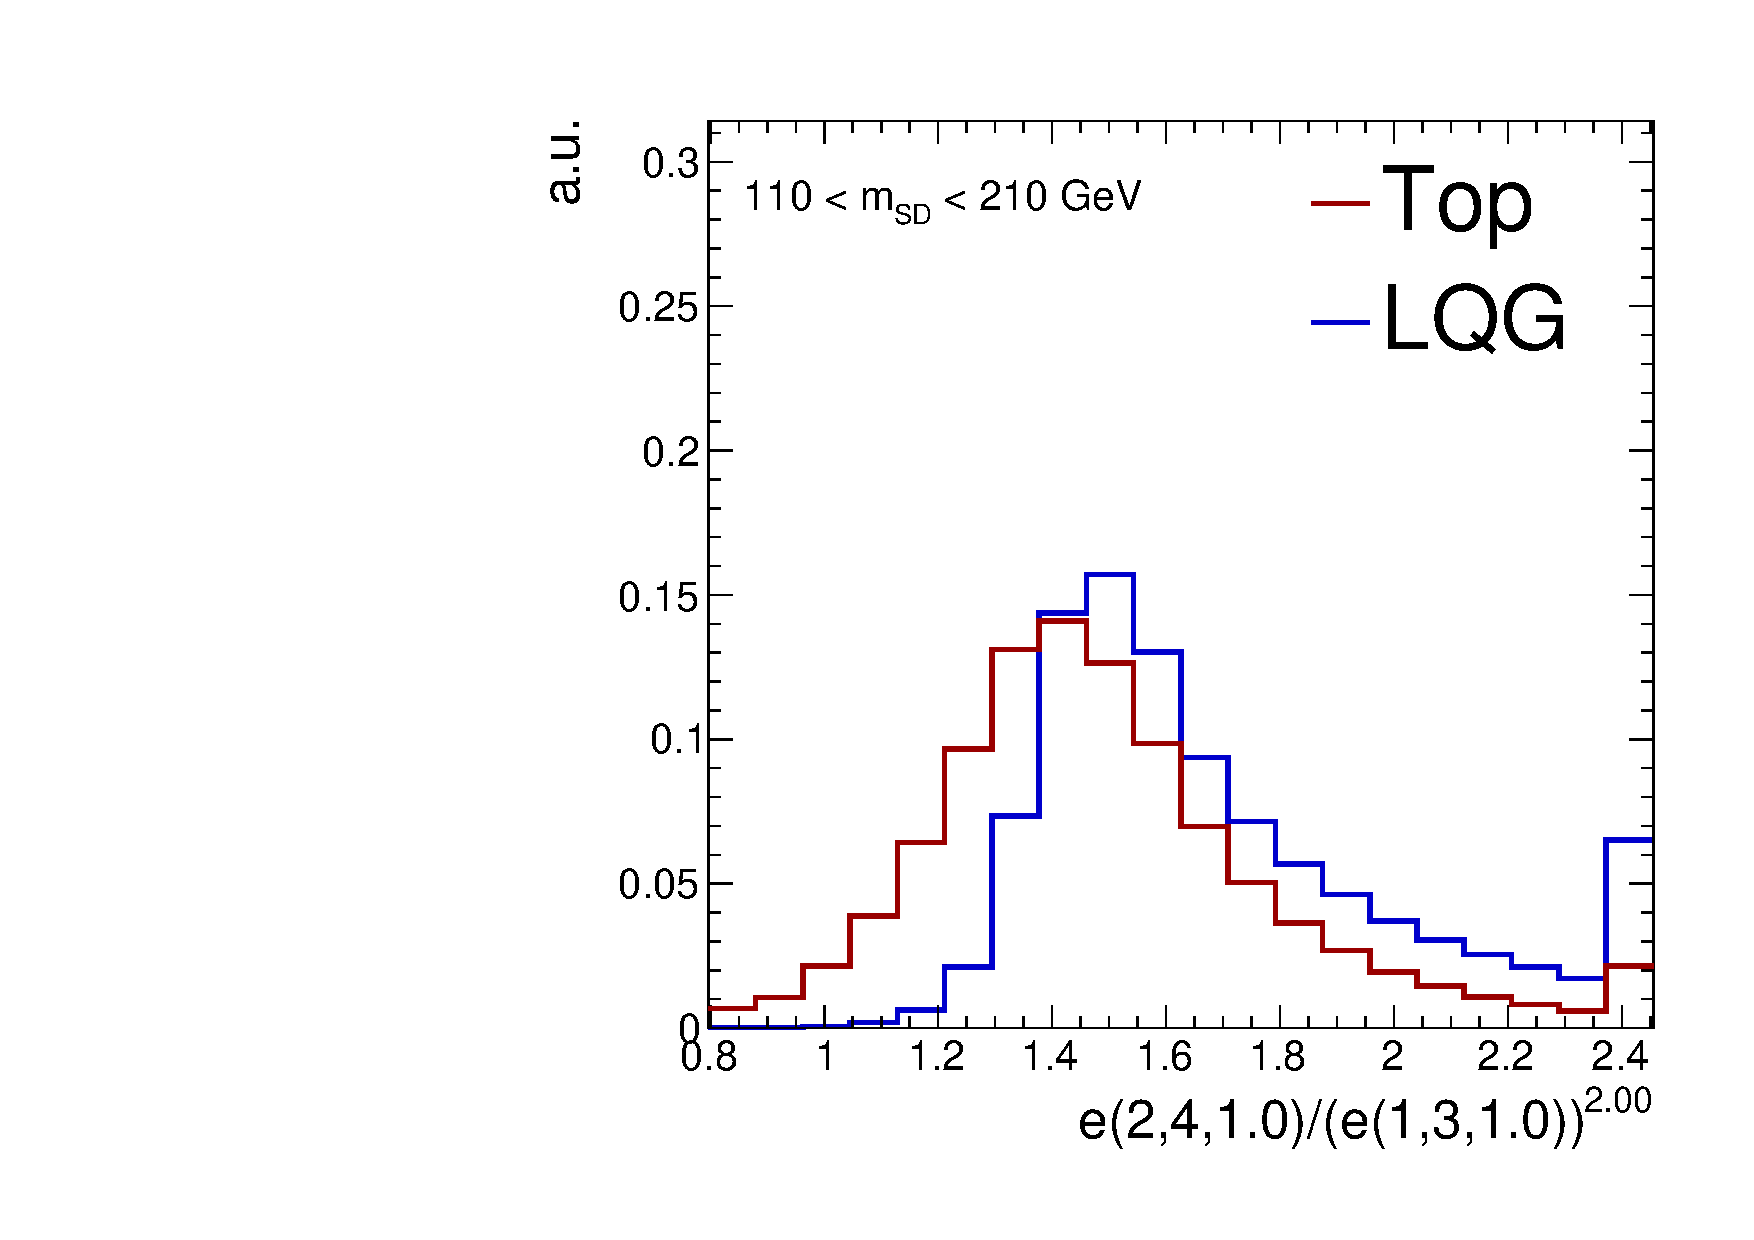
\includegraphics[width=0.24\textwidth]{figures/toptagging/shapes/mass_ratio_24101310.pdf}
        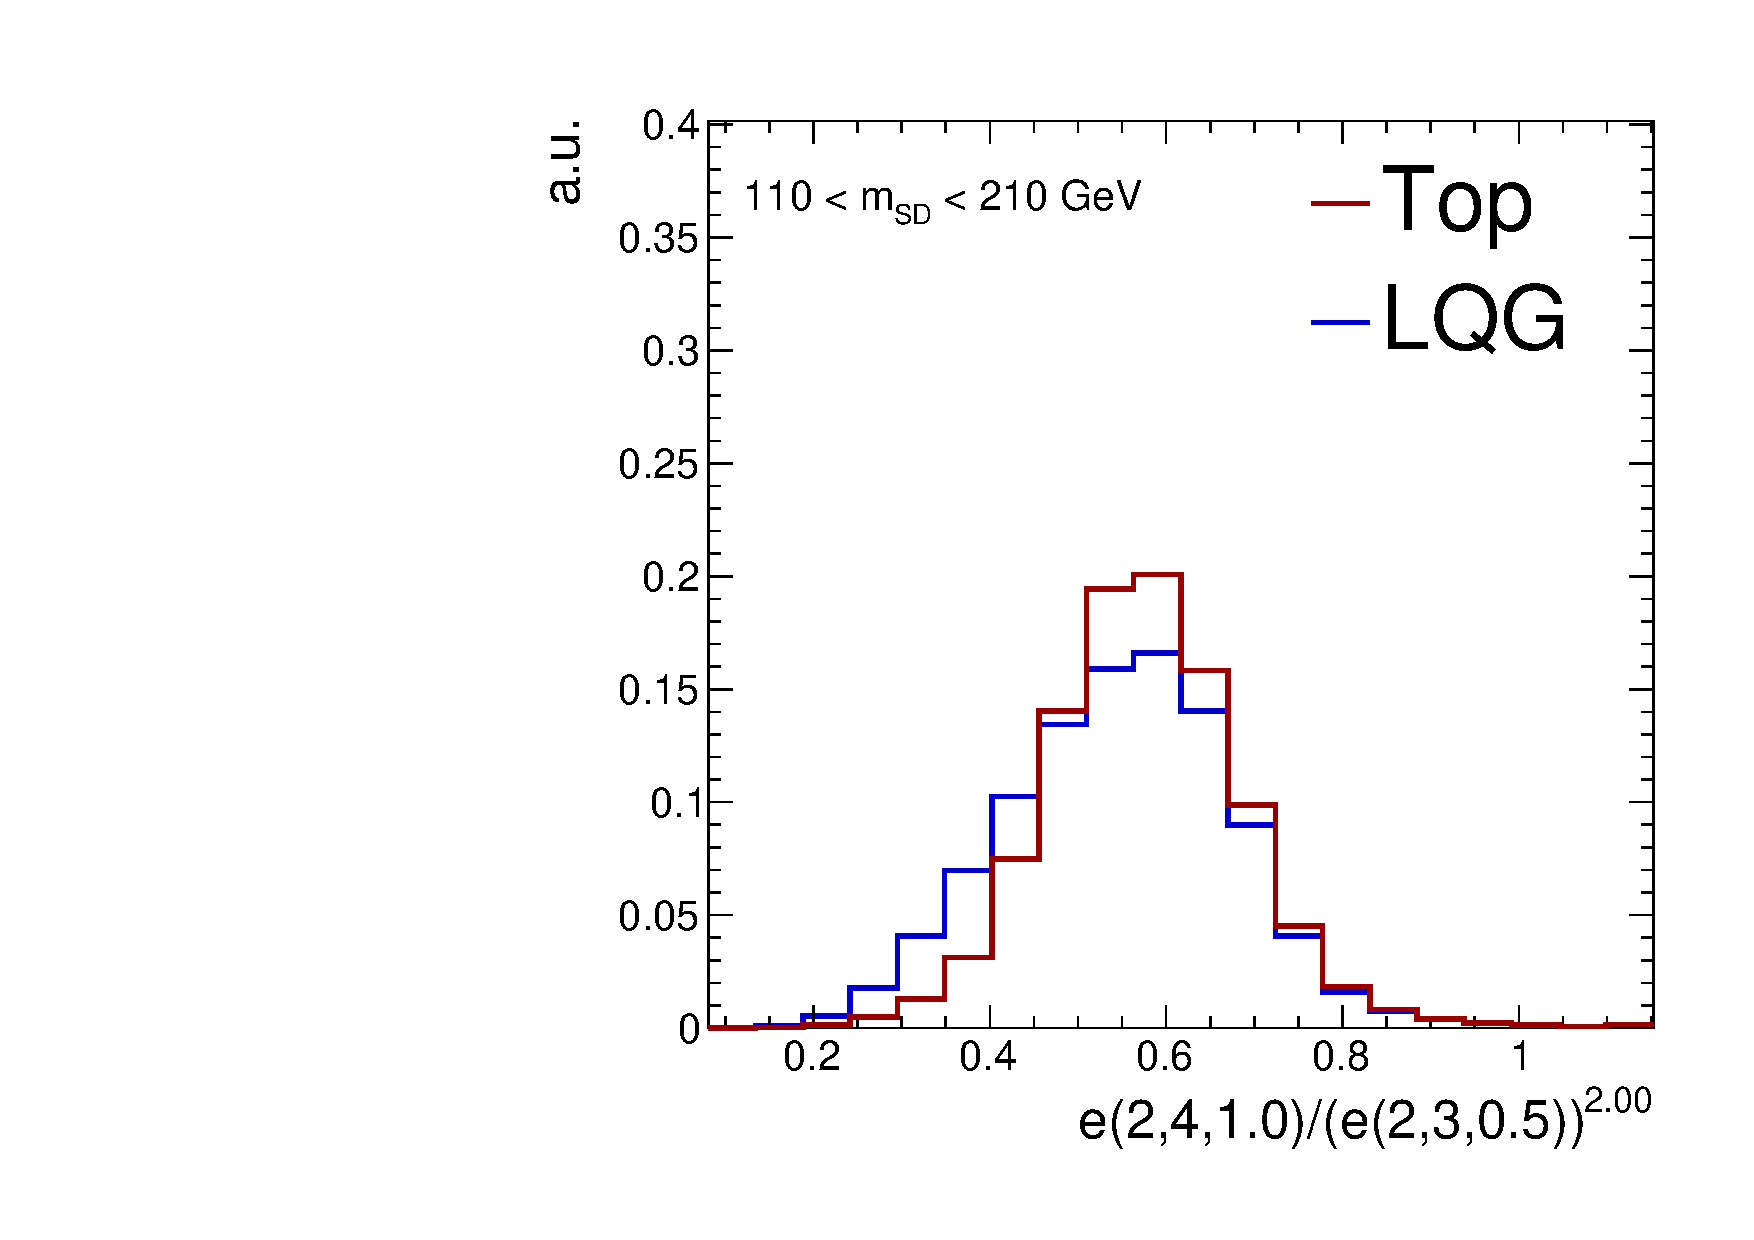
\includegraphics[width=0.24\textwidth]{figures/toptagging/shapes/mass_ratio_24102305.pdf}
        \includegraphics[width=0.24\textwidth]{figures/toptagging/shapes/mass_ratio_24201320.pdf}
        \includegraphics[width=0.24\textwidth]{figures/toptagging/shapes/mass_ratio_12201210.pdf}
        \includegraphics[width=0.24\textwidth]{figures/toptagging/shapes/mass_ratio_13402320.pdf}
        \includegraphics[width=0.24\textwidth]{figures/toptagging/shapes/mass_ratio_33101340.pdf}
        \includegraphics[width=0.24\textwidth]{figures/toptagging/shapes/mass_ratio_33102320.pdf}
        \includegraphics[width=0.24\textwidth]{figures/toptagging/shapes/mass_ratio_33203340.pdf} \\ 
        \includegraphics[width=0.24\textwidth]{figures/toptagging/shapes/mass_fjTau32SD.pdf}
        \includegraphics[width=0.24\textwidth]{figures/toptagging/shapes/mass_fjHTTFRec.pdf}
        \caption{Distributions of the 13 features selected by the iterative BDT training}
        \label{figs:jets:features}
    \end{center}
\end{figure}

\begin{figure}[]
    \begin{center}
        \includegraphics[width=0.5\textwidth]{figures/toptagging/bdt/massCut_roc.pdf}
        \caption{Receiver Operating Characteristic (ROC) curve comparing various top identification methods. The ``Combined BDT'' is the ID method chosen as the final tagger.}
        \label{figs:jets:roc}
    \end{center}
\end{figure}

\section{Data validation}
\label{sec:jets:sf}

Prior to using the top BDT to identify top jets and reject LQG jets, we must verify that the simulation describes the BDT distribution properly as compared to data, and correct for any residual discrepancies.
Figure~\ref{fig:jets:bdtdist} shows the BDT response and $m_\SD$ in top- and LQG-enriched selections.
Top quarks are isolated by selecting events that produce $t\bar{t}$ pairs, in which one top quark decays hadronically (the top jet) and the other decays muonically ($t\rightarrow b\mu^+\nu_mu$).
The leptonic $t$ is selected by identifying the muon and $b$ jet. 
We further require that the CA15 jet have $110<m_\SD<210$ GeV and at least one SD subjet to be $b$-tagged.
LQG jets are selected by using $Z(\rightarrow\mu\mu)$+jet events.
We require two opposite sign muons, with $|m_{\mu\mu}-m_Z|<30$ GeV; this selection selects a $\gtrsim95\%$ pure $Z$+jet sample. 
In both samples, we observe reasonably good agreement between data and simulation.

\begin{figure}[]
    \begin{center}
        \begin{subfigure}[t]{\textwidth}
    \begin{center}
            \includegraphics[width=0.35\textwidth]{figures/toptagging/sf/dimuon_fjMSD_logy.pdf}
            \includegraphics[width=0.35\textwidth]{figures/toptagging/sf/dimuon_top_ecf_bdt.pdf}
            \caption{Dimuon selection}
    \end{center}
        \end{subfigure} \\ 
        \begin{subfigure}[t]{\textwidth}
    \begin{center}
            \includegraphics[width=0.35\textwidth]{figures/toptagging/sf/singlemuontop_fjMSD.pdf}
            \includegraphics[width=0.35\textwidth]{figures/toptagging/sf/singlemuontop_top_ecf_bdt.pdf}
            \caption{$t\bar{t}$ selection}
    \end{center}
        \end{subfigure}
        \caption{Comparison of the BDT response and jet mass in data and simulation, in top and LQG jets.}
        \label{fig:jets:bdtdist}
    \end{center}
\end{figure}

To account for any remaining differences, we define a scale factor (SF):
\begin{equation}
    \mathrm{SF}(x) = \frac{\epsilon_\mathrm{Data}(\mathrm{BDT}>x \text{ and }110<m_\SD<210)}{\epsilon_\mathrm{MC}(\mathrm{BDT}>x \text{ and }110<m_\SD<210)}
\end{equation}
where $x$ is a particular decision boundary and $\epsilon$ is the fraction of data or MC events passing this BDT  and mass selection.
These are chosen to optimize sensitivity to the mono-top analysis, as described in Chapter~\ref{sec:mt}.
The SF is strongly dependent on the type of jet; in particular, we expect different SFs for top and LQG jets.
In what follows, we will define two decision boundaries: a loose (0.1) and a tight (0.45) category.

To compute $\mathrm{SF}_\mathrm{LQG}$, we use the dimuon selection in Figure~\ref{fig:jets:bdtdist}, as this contains an essentially pure selection of LQG jets.
Two sources of uncertainty are considered: the statistical uncertainties present in the data and MC, and the uncertainties on the theoretical prediction of the cross section of the small non-LQG backgrounds ($t\bar{t}$ and diboson events).
The measured SFs are:
\begin{align}
    \mathrm{SF}_\mathrm{LQG}(0.1) = 1.02 & \pm 0.05 (\mathrm{total}) \nonumber \\ 
                                         & \pm 0.04 (\mathrm{statistical}) \pm 0.03 (t\bar{t}+\mathrm{diboson}) \nonumber \\ 
    \mathrm{SF}_\mathrm{LQG}(0.45) = 0.97 & \pm 0.07 (\mathrm{total}) \nonumber \\ 
                                         & \pm 0.06 (\mathrm{statistical}) \pm 0.03 (t\bar{t}+\mathrm{diboson})
\end{align}

The process for top jets is complicated by the fact that the top pair selection in Figure~\ref{fig:jets:bdtdist} is not sufficiently pure in merged top jets.
There is significant contamination from $W$+jets events.
Furthermore, we cannot ensure that every $t\bar{t}$ event selected produces a \emph{merged} top jet - some events may contain jets in which only part of the top's decay products are clustered into the CA15 jet.
Therefore, we extract the efficiency by means of a template fit to the mass distribution of passing and failing events, which can separate the top and LQG components in the selection.
It is for this reason that we only use groomed observables in the BDT: grooming prevents a strong correlation between the observables and $m_\SD$.
Such a correlation would cause the mass distribution of passing LQG jets to be indistinguishable from that of passing top jets.
Figure~\ref{fig:jets:sffits} show the fits in the passing and failing regions for both decision boundaries.

\begin{figure}[]
    \begin{center}
        \begin{subfigure}[t]{\textwidth}
    \begin{center}
            \includegraphics[width=0.35\textwidth]{figures/toptagging/sf/loose_fail.pdf}
            \includegraphics[width=0.35\textwidth]{figures/toptagging/sf/loose_pass.pdf}
            \caption{Loose BDT-tagged}
    \end{center}
        \end{subfigure}
        \begin{subfigure}[t]{\textwidth}
    \begin{center}
            \includegraphics[width=0.35\textwidth]{figures/toptagging/sf/tight_fail.pdf}
            \includegraphics[width=0.35\textwidth]{figures/toptagging/sf/tight_pass.pdf}
            \caption{Tight BDT-tagged}
    \end{center}
        \end{subfigure}
        \caption{Fits to the $m_\SD$ distribution in a $t\bar{t}$ sample to extract the efficiency in data of the BDT and mass selections.
                 All uncertainties plotted and quoted are statistical in nature.}
        \label{fig:jets:sffits}
    \end{center}
\end{figure}

Several sources of uncertainty are considered for this measurement:
\begin{itemize}
    \item Poisson uncertainties in the data and simulation 
    \item CA15 jet energy scale and resolution 
    \item Definition used to select ``merged top'' jets, allowing $\max \Delta R_{qq'}$ to vary between 1 and 1.5 (nominal value is 1.2)
    \item Efficiency of selecting $b$ jets
\end{itemize}
The resultant SFs and associated uncertainties are:
\begin{align}
    \mathrm{SF}_\mathrm{top}(0.1) = 1.08 & \pm 0.04 (\mathrm{total}) \nonumber \\ 
                                         & \pm 0.03 (\mathrm{statistical}) \pm 0.02 (\mathrm{JES+JER}) \pm 0.02 (\mathrm{merging}) \pm 0.002 (b) \nonumber \\ 
    \mathrm{SF}_\mathrm{top}(0.45) = 1.07 & \pm 0.06 (\mathrm{total}) \nonumber \\ 
                                         & \pm 0.03 (\mathrm{statistical}) \pm 0.02 (\mathrm{JES+JER}) \pm 0.014 (\mathrm{merging}) \pm 0.000 (b) 
\end{align}


\boldmath
\chapter{The Search for Missing Momentum and a Top Quark}
\unboldmath
\label{sec:mt}

In this chapter, we discuss the search for dark matter produced in association with a single top quark (\emph{mono-top}).
Since the initial state of $pp$ collisions do not contain any appreciable contribution from top quarks, any process that produces a single top quark must involve some flavor violation.
In the Standard Model, any such process is heavily suppressed by off-diagonal elements of the CKM matrix.
The SM production mechanism for the mono-top signature (Figure~\ref{fig:mt:tzq}) involves a $b$ quark in the final state, and thus does not couple the third generation with the first or second.
True production of mono-top must introduce some such coupling as an extension to the SM, in addition to one (or more) invisible particle to serve as a DM candidate.

\begin{figure}[]
    \begin{center}
        \includegraphics[width=0.5\textwidth]{figures/monotop/diagrams/tzq.pdf}
        \caption{Production of mono-top in the SM, in which a top quark is produced in addition to a $Z$ boson and bottom quark. The $Z$ decays to neutrinos, providing large \ptmiss.}
        \label{fig:mt:tzq}
    \end{center}
\end{figure}

We introduce two DM models that can produce this final state: a flavor-changing neutral current $V$ and a charged, colored scalar $\phi$.
These models will also be used to benchmark the sensitivity of the analysis.
However, it should be emphasized that the search is motivated and designed without reliance on any specific model; the assumption is that the mono-top final state alone is indicative of new physics, regardless of the specific production mechanism.

The flavor-changing neutral current (FCNC) $V$ is assumed to couple to a fermionic DM candidate $\chi$.
A partial Lagrangian of the interaction terms is given by:
\begin{equation}
\mathcal{L}_\text{int}=  V_\mu  \overline\chi \gamma^\mu (  g^V_{\chi} + g^A_{\chi} \gamma_5 ) \chi
                           + \overline{q}_u \gamma^\mu
                           ( g^V_u + g^A_u \gamma_5 ) q_u V_\mu
                           + \overline{q}_{d} \gamma^\mu
                           (  g^V_{d} + g^A_{d} \gamma_5 ) q_d V_\mu
                           + \text{h.c.},
    \label{eq:Lfcnc}
\end{equation}
The model comes with 22 free parameters, broadly organized in three sets:
\begin{itemize}
    \item The masses $m_V$ and $m_\chi$. (2)
    \item The couplings $g_\chi^V$ and $g_\chi^A$. These, respectively, control the strength of the vector and axial interactions between $V$ and $\chi$. (2)
    \item The four coupling matrices $g_{q}^{X}$, where $q=u,d$ and $X=V,A$.
          As before, $X$ determines the type of spin-1 interaction.
          In principle, different coupling strengths can be permitted for up- and down-type quarks, so this indexed by $q$.
          Each $g_{q}^{X}$ is a $3\times3$ matrix, cross-coupling the three quark generations.
          To preserve $\mathrm{SU}(2)_\mathrm{L}$ symmetry, we require $g_u^V - g_u^A = g_d^V - g_d^A$. ($3\times6=18$)
\end{itemize}

It is the $g_{u,d}^{V,A}$ matrices that determine whether the model can produce mono-top, or mono-bottom, or mono-up, etc.
If $g_{u,d}$ is strongly diagonal, in the sense that the cross-generation couplings are weak, then mono-light quark production will dominate, resulting in the mono-jet final state (Figure~\ref{fig:mt:fcncdiaga}).
On the other hand, if we assume the only non-zero elements are those that couple the first and third generations, then mono-top production at the LHC is the best way to probe this model (Figure~\ref{fig:mt:fcncdiagb}).
It is this latter choice that will be made in the rest of this chapter; other choices are best probed using a combination of multiple DM channels, which is left as future work.
Furthermore, to respect $\mathrm{SU}(2)_\mathrm{L}$ symmetry, we make the assumption that $g_u^V = g_d^V$ and $g_u^A = g_d^A$.

\begin{figure}[]
    \begin{center}
        \begin{subfigure}[t]{0.49\textwidth}
            \includegraphics[width=\textwidth]{figures/monotop/diagrams/mj.pdf}
            \caption{$(g_{u}^{V,A})_{ij} \approx \delta_{ij}$}
            \label{fig:mt:fcncdiaga}
        \end{subfigure}
        \begin{subfigure}[t]{0.49\textwidth}
            \includegraphics[width=\textwidth]{figures/monotop/diagrams/fcncb.pdf}
            \caption{$(g_{u}^{V,A})_{ij} \approx \delta_{i1}\delta_{j3} + \delta_{i3}\delta_{j1}$}
            \label{fig:mt:fcncdiagb}
        \end{subfigure}
        \caption{Possible DM production at the LHC, assuming a simplified spin-1 extension to the SM.
                 The shown diagrams are at LO, although the MC simulation of these processes is at NLO in QCD vertices.}
        \label{fig:mt:fcncdiag}
    \end{center}
\end{figure}

In the second benchmark model, the charged, colored scalar $\phi$ couples to down-type quarks, or to a fermionic DM candidate $\psi$ and a top quark.
The interaction terms of the Lagrangian is given by:
\begin{equation}
    \mathcal{L}_\text{int} = \phi\overline{{d}}_i^C[(a_{q})^{ij}+(b_{q})^{ij}\gamma^5]{d}_j+\phi\overline{{t}}[a_{\psi}+b_{\psi}\gamma^5]\psi+\text{h.c.}
\end{equation}
There are 16 free parameters in this model, broadly organized in three categories:
\begin{itemize}
    \item The masses $m_\phi$ and $m_\psi$. (2)
    \item The couplings at the $\phi \bar{t} \psi$ vertex $a_\psi$ and $b_\psi$, which respectively control the strength of the scalar and pseudoscalar interactions. (2)
    \item The couplings at the $\phi \bar{d_i} d_j$ vertex $a_q^{ij}$ and $b_q^{ij}$ where $i,j=1,2,3$. Again, $a$ and $b$ refer the scalar and pseudoscalar couplings, respectively. (12)
\end{itemize}
In this model, mono-top production primarily occurs through the resonant decay of $\phi$ to $\psi$ and $t$, as shown in Figure~\ref{fig:mt:resdiag}.

\begin{figure}[]
    \begin{center}
        \includegraphics[width=0.5\textwidth]{figures/monotop/diagrams/resonant.pdf}
        \caption{Possible DM production at the LHC, assuming the existence of a charged, color scalar that couples to DM and the top quark.
                 The diagrams and the MC simulation of this process are at LO.}
        \label{fig:mt:resdiag}
    \end{center}
\end{figure}

The two benchmark models show markedly different spectra in Figure~\ref{fig:mt:shapes}, motivating their use to test different modes of mono-top production.
The FCNC produces a falling \ptmiss~distribution.
The decay of a scalar resonance produces a distribution peaking at approximately $\ptmiss\approx\nicefrac{m_\phi}{2}$.
This is because \ptmiss~is the transverse component of the momentum of one of the decay products of the resonance.
In the region of interest, $m_\phi$ is quite large and the scalar is produced near rest, and so $|\vec p_\psi| \sim \nicefrac{m_\phi}{2}$.

\begin{figure}[]
    \begin{center}
        \begin{subfigure}[t]{0.49\textwidth}
            \includegraphics[width=\textwidth]{figures/monotop/diagrams/fcnc_pfmet.pdf}
            \caption{FCNC}
        \end{subfigure}
        \begin{subfigure}[t]{0.49\textwidth}
            \includegraphics[width=\textwidth]{figures/monotop/diagrams/res_pfmet.pdf}
            \caption{Scalar resonance}
        \end{subfigure}
        \caption{Spectra of DM (missing) momentum under various signal hypothesis.
                 In the FCNC case, the spectra become harder as $m_V$ increases, as the momentum transfer needed to produce a particle of mass $m_V$ increases.
                 In the scalar resonance case, the \ptmiss~distribution is a Jacobian shape, with a peak near half the resonance mass. }
        \label{fig:mt:shapes}
    \end{center}
\end{figure}

\clearpage

\section{Signal selection}
\label{sec:mt:sel}

In this section, we will describe how events with large missing momentum and a top jet candidate are selected, and events with other signatures, such as leptons and photons, are rejected.
The selection begins with a relatively loose trigger definition, to record collision events, followed by a more stringent set of \emph{offline} criteria and categorization.

When looking at events that pass a simple set of criteria (moderate $\ptmiss$ and one CA15 jet), it is clear (Figure~\ref{fig:mt:bkgshapes}) that the highest signal sensitivity is found in regions of high $\ptmiss$ and jet $\pt$.
After this loose selection, the three primary backgrounds, from most to least important, are:
\begin{itemize}
    \item $Z\rightarrow\nu\nu$. 
          When the $Z$ is produced in association with one or more jets, the jet system will, in rare cases, pass the criteria used to select a top jet. 
          The neutrinos manifest as $\ptmiss$.
    \item $W\rightarrow\ell\nu$. 
          As in the case of the $Z$, additional jets mimic the signature of a top jet. 
          Typically, the charged lepton in the final state is vetoed, but if it is out of acceptance ($e,\mu$) or fails ID criteria ($\tau_\mathrm{h}$), then it is not identified.
    \item $t\bar{t} \rightarrow bq\bar{q}' + \bar{b}\ell\nu$. 
          As in the case of the $W$, a charged lepton in the final state may not be properly identified. 
          Unlike the previous two processes, a semi-leptonic $t\bar{t}$ event contains a real hadronic top quark decay.
\end{itemize}

\begin{figure}[]
    \begin{center}
        \begin{subfigure}[t]{0.49\textwidth}
            \includegraphics[width=\textwidth]{figures/monotop/shapes/signal_pfmet_logy.pdf}
            \caption{Missing momentum}
        \end{subfigure}
        \begin{subfigure}[t]{0.49\textwidth}
            \includegraphics[width=\textwidth]{figures/monotop/shapes/signal_fjPt_0__logy.pdf}
            \caption{Jet $\pt$}
        \end{subfigure}
        \caption{Comparison of missing and jet momenta in various backgrounds and signal models.}
        \label{fig:mt:bkgshapes}
    \end{center}
\end{figure}

\subsection{Online trigger selection}
\label{sec:mt:trigger}

Data events are first selected by the L1 trigger system by requiring $p_\mathrm{T,L1}^\mathrm{miss} > 70$ GeV, where:
\begin{equation}
    p_\mathrm{T,L1}^\mathrm{miss} = -\left(\sum_{i\in C} \vec{p}_i \right)_\mathrm{T}, \text{ $C = \{$calorimeter deposits with $|\eta|<3.0\}$}
\end{equation}
Events that pass this selection are sent to the HLT system, where we place requirements on the both the missing momentum ($p_\mathrm{T,HLT}^\mathrm{miss}$) and the missing hadronic momentum ($H_\mathrm{T,HLT}^\mathrm{miss}$).
These are defined as:
\begin{equation}
    p_\mathrm{T,HLT}^\mathrm{miss} = -\left(\sum_{i\in\mathrm{particles}} \vec{p}_i \right)_\mathrm{T}, \text{ all particles except muons}
\end{equation}
\begin{equation}
    H_\mathrm{T,HLT}^\mathrm{miss} = -\left(\sum_{i\in\mathrm{jets}} \vec{p}_i \right)_\mathrm{T}, \text{ jets passing noise-rejection ID}
\end{equation}
The HLT decides to keep an event if $\min(p_\mathrm{T,HLT}^\mathrm{miss}, H_\mathrm{T,HLT}^\mathrm{miss})$ is higher than a specified threshold.
Over the course of the data-taking period considered in this chapter, this threshold varied from $90$ to $120$ GeV.
The use of noise-rejection in the definition of $H_\mathrm{T,HLT}^\mathrm{miss}$ makes it more resilient to detector noise than $p_\mathrm{T,HLT}^\mathrm{miss}$.
Therefore, we place symmetric selections on both quantities.

Note that in all trigger decisions, muons are excluded from the missing momentum calculations.
This means that an event which produces high-momentum muons can be selected using these triggers.
This flexibility will be exploited in Section~\ref{sec:mt:bkg}. 
Missing momentum with and without muons are treated on equal footing by defining the \emph{hadronic recoil} $U$:
\begin{equation}
    \vec{U} = \vptmiss + \sum_{\ell\in\text{ lep.}} \vec{p}_\mathrm{T}^\ell + \sum_{\gamma\in\text{ photons}} \vec{p}_\mathrm{T}^\gamma
    \label{eq:mt:u}
\end{equation}
where \emph{lep} refers to all identified electrons and muons.
In an event without electrons, muons and photons, $U = \ptmiss$.

Since the online environment and reconstruction are significantly limited as compared to the offline reconstruction of $U$, we do not expect the trigger decision to be a step function at $U=120$ GeV.
Therefore, we define and measure a trigger efficiency:
\begin{equation}
    \epsilon_\mathrm{trig} (U) = \frac{N_\text{pass trig}(U)}{N(U)}
\end{equation}
This is measured using $W\rightarrow\mu\nu$ events containing one or more high-$\pt$ jets.
The events are triggered using single-$\mu$ triggers, which have lower thresholds and efficiencies close to 1 in this phase space.
We then require events have exactly one well-identified muon and at least one jet with $\pt>100$ GeV.
Figure~\ref{fig:mt:trigeff} shows the efficiency as a function of $U$.
A threshold of $U>250$ GeV is chosen to optimize the tradeoff between the number of selected signal events and the increased systematic uncertainties incurred from the steeply-rising part of the efficiency curve.

\begin{figure}[]
    \begin{center}
        \includegraphics[width=0.49\textwidth]{figures/monotop/trigger/trigeff_nmu1pfUWmag.pdf}
        \caption{Efficiency of the $\ptmiss$ trigger measured in single-muon events. }
        \label{fig:mt:trigeff}
    \end{center}
\end{figure}

\subsection{Offline signal selection}

The signal regions (SRs) are defined by a further set of offline selection criteria, which are listed and motivated in Table~\ref{tab:mt:cuts}.
The selections are optimized on the basis of sensitivity to a benchmark signal hypothesis, an FCNC with $m_V=1.7$ TeV.
This optimization is approximately ideal for all relevant signal models, as the main differences are in the tail of the $\ptmiss$ distribution, which is not affected by the criteria in Table~\ref{tab:mt:cuts}.
As described in Section~\ref{sec:jets:reco}, two working points (WPs) are defined for the top ID BDT.
The signal events passing all other selection criteria are partitioned into a \emph{loose} SR and a \emph{tight} SR on the basis of which WP the top candidate jet satisfies.

\begin{table}[]
    \caption{Criteria used to select events for the mono-top search signal regions. Note that two SRs are defined, based on the BDT score.}
    \label{tab:mt:cuts}
    \begin{tabular}{p{0.4\textwidth}p{0.6\textwidth}}
        Criterion & Notes \\
        \hline
        \hline
        $\ptmiss>250$ GeV & Signal events should have large missing momentum. Exact threshold is chosen to maximize online trigger efficiency. \\
        1 CA15 jet with $\pt>250$ GeV & Top quark candidate. Recoils against $\ptmiss$, so threshold is set at $250$ GeV. \\
        CA15 jet $110 < m_\mathrm{SD} < 210$ GeV & Consistency with top quark mass. \\
        At least one $b$-tagged sub-jet & Identifying $b$ hadron produced from top decay/hadronization. \\
        No $b$-tagged narrow jets & Rejecting semi-leptonic $t\bar{t}$ decays. \\
        \hline
        No identified $e,\mu,\tau_\mathrm{h}$ & Suppress $W$+jet and $t\bar{t}$ processes. \\
        No identified $\gamma$ & Suppress $\gamma$+jet processes. \\
        \hline
        $\min_\mathrm{jets}\Delta\phi(\mathrm{jet},\ptmiss) > 0.5$ & Remove events with large $\ptmiss$ caused by mismeasured jets. \\
        \hline
        CA15 jet BDT & Identifying top decay structure. If the jet passes the tight WP, it is placed in the \emph{tight} SR. Otherwise, if it only passes the loose WP, it is placed in the \emph{loose} SR.\\
    \end{tabular}
\end{table}

Figure~\ref{fig:mt:prefit_signal} shows the $\ptmiss$ distributions, as predicted by MC and as observed in collected data, in the two signal regions.

\begin{figure}[]
    \begin{center}
        \begin{subfigure}[t]{0.49\textwidth}
            \includegraphics[width=\textwidth]{figures/monotop/prefit/signal_loose_pfmet_logy.pdf}
            \caption{Loose SR}
        \end{subfigure}
        \begin{subfigure}[t]{0.49\textwidth}
            \includegraphics[width=\textwidth]{figures/monotop/prefit/signal_tight_pfmet_logy.pdf}
            \caption{Tight SR}
        \end{subfigure}
        \caption{$\ptmiss$ distributions in the two mono-top signal regions.
                 The bottom section of each figure shows the ratio of the data and the prediction.
                 The only uncertainties plotted in these figures are those arising from Poisson fluctuations in data (black bars) and MC (grey band).
                 Enough MC events are produced such that the MC statistical uncertainties are smaller than those in data.}
        \label{fig:mt:prefit_signal}
    \end{center}
\end{figure}

\clearpage

\section{Background estimation}
\label{sec:mt:bkg}

Searching for DM amounts to looking for an excess of data events over the SM prediction at large values of $\ptmiss$.
Therefore, the $\ptmiss$ distribution of the three primary SM backgrounds described in Section~\ref{sec:mt:sel} must be predicted with small uncertainty.
The MC simulation provides a reasonable description of the data, but the theoretical uncertainties inherent in the MC, primarily due to higher-order QCD effects, can range up to $20\%$.
To reduce the prediction uncertainty, data samples that cannot contain a DM signal (\emph{control} data) is used to directly estimate or supplement the estimation of SM processes in the SR.
This approach is known as \emph{data-driven} estimation.

The basic strategy is as follows: each invisible background will be constrained by one or more visible processes for which we can measure the $U$ spectrum.
The visible processes are chosen such that they are sufficiently similar to the targeted background, minimizing the uncertainties in the extrapolation.
The $\ttbar$ background is estimated using $\ttbar$ events in which the charged lepton is properly reconstructed.
The $Z$ and $W$ backgrounds are simultaneously constrained using a combination of $Z\rightarrow\ell\ell$, $W\rightarrow\ell\nu$, and $\gamma$ events.
Extrapolations which link very similar processes, such as $Z\rightarrow\mu\mu$ and $Z\rightarrow\nu\nu$, can be made with relatively small experimental uncertainties.
The linkage of dissimilar processes, such as $\gamma$ and $Z\rightarrow\nu\nu$, additionally brings relatively large theoretical uncertainties, which must be carefully estimated.

\subsection{Visible final states to constrain invisible final states}

As a starting point, let us tackle the estimation of $Z\rightarrow\nu\nu$ in the SR.
Since the momentum imbalance (up to experimental effects) in a $Z\rightarrow\nu\nu$ event is just the transverse momentum of the $Z$ boson ($\pt^Z$), we must estimate $\pt^Z$.
To good approximation, the $\pt^Z$ distribution is independent of the decay mode of the $Z$ boson.
Therefore, it is natural to estimate $\ptmiss(Z\rightarrow\nu\nu)$ by measuring $\pt^Z(Z\rightarrow\mu\mu)$, as muons are easily identifiable and reconstructible.

However, there is one important distinction between $\nu\nu$ and $\mu\mu$ events.
In the latter, $\pt^Z$ can be directly measured, whereas in the former it must be inferred through a momentum imbalance.
Effects like jet energy scale impact $\ptmiss$, but not $\pt^{\mu\mu}$.
Therefore, instead of directly measuring $\pt^{\mu\mu}$ in $\mu\mu$ events, we use the hadronic recoil $U$.
In SR events, in which there are no $e,\mu,\gamma$, $U = \ptmiss$.
In $Z\rightarrow\mu\mu$ events, $U$ mimics the momentum imbalance, if we had pretended the identified muons did not exist when computing $\ptmiss$.
Therefore, $U$ is an exact analogy for $\ptmiss$ in the SR.
Figure~\ref{fig:mt:zvsz} makes the same argument in a schematic fashion.

\begin{figure}[]
    \begin{center}
        \begin{subfigure}[t]{0.49\textwidth}
            \includegraphics[width=\textwidth]{figures/monotop/diagrams/zsr.pdf}
            \caption{$Z\rightarrow\nu\nu$}
        \end{subfigure}
        \begin{subfigure}[t]{0.49\textwidth}
            \includegraphics[width=\textwidth]{figures/monotop/diagrams/zcr.pdf}
            \caption{$Z\rightarrow\mu\mu$}
        \end{subfigure}
        \caption{Schematic representation of two $Z$ decay modes: to neutrinos (as in the SR) and to muons (as in the CRs).
                 Note that in both cases, $U$ is sensitive to the same effects arising from the measurement of the jet recoiling against the $Z$ boson, whereas $\pt^{\mu\mu}$ is largely independent of the jet.}
        \label{fig:mt:zvsz}
    \end{center}
\end{figure}

Table~\ref{tab:mt:zmm_cuts} describes the criteria used to define events in the \emph{$\mu\mu$} control regions (CRs).
Figure~\ref{fig:mt:prefit_dimuon} shows the distribution of $U$ in these CRs, as well as the $m_{\mu\mu}$ and $\pt^\mu$ distributions.

\begin{table}[]
    \caption{Criteria used to select events for the mono-top $Z\rightarrow\mu\mu$ CR. As in the SR, the region is further subdivided based on the jet BDT score.}
    \label{tab:mt:zmm_cuts}
    \centering
    \begin{tabular}{p{0.4\textwidth}p{0.6\textwidth}}
        Criterion & Notes \\
        \hline
        \hline
        $U>250$ GeV & Same as the SR selection, so as to select $Z$s in the same phase space. \\
        1 CA15 jet with $\pt>250$ GeV &  Same as SR \\
        CA15 jet $110 < m_\mathrm{SD} < 210$ GeV & Same as SR \\
        \hline
        Well-identified $\mu^-,\mu^+$ pair, with $|m_{\mu\mu}-m_Z|<30$ GeV & Identifying the $Z\rightarrow\mu\mu$ resonance. \\
        No identified $e,\tau_\mathrm{h}$ & Same as SR. \\
        No identified $\gamma$ & Same as SR \\
        \hline
        $\min_\mathrm{jets}\Delta\phi(\mathrm{jet},U) > 0.5$ & Same as SR \\
        \hline
        CA15 jet BDT & Same as SR\\
    \end{tabular}
\end{table}

\begin{figure}[]
    \begin{center}
        \begin{subfigure}[t]{0.49\textwidth}
            \includegraphics[width=\textwidth]{figures/monotop/prefit/dimuon_loose_pfUZmag_logy.pdf}
            \caption{$U$ in loose CR}
        \end{subfigure}
        \begin{subfigure}[t]{0.49\textwidth}
            \includegraphics[width=\textwidth]{figures/monotop/prefit/dimuon_tight_pfUZmag_logy.pdf}
            \caption{$U$ in tight CR}
        \end{subfigure}
        \begin{subfigure}[t]{0.49\textwidth}
            \includegraphics[width=\textwidth]{figures/monotop/prefit/dimuon_loose_diLepMass_logy.pdf}
            \caption{$m_{\mu\mu}$}
        \end{subfigure}
        \begin{subfigure}[t]{0.49\textwidth}
            \includegraphics[width=\textwidth]{figures/monotop/prefit/dimuon_loose_looseLep1Pt_logy.pdf}
            \caption{Leading muon $\pt$}
        \end{subfigure}
        \caption{Various kinematic distributions in the two mono-top $\mu\mu$ CRs.
                 All predicted distributions are prior to the maximization of the likelihood, and the grey band refers only to the statistical uncertainty of the MC.
                 The pre-fit MC describes the observed data reasonably well.
                 }
        \label{fig:mt:prefit_dimuon}
    \end{center}
\end{figure}

The control data is used to constrain the SR prediction by means of \emph{transfer factors} $\Ti{X}{Y}$, where $X$ refers to a particular CR (e.g. $\mu\mu$), $Y$ refers to a particular process (e.g. $Z$), and $i$ refers to a particular bin in the CR (e.g. $200<U<250$ GeV in the tight category).
Formally:
\begin{equation}
    \Ti{\mu\mu}{Z} = \frac{N^\mathrm{SR}_i(Z\rightarrow\nu\nu)}{N^{\mu\mu}_i(Z\rightarrow\mu\mu)}
\end{equation}
The transfer factors are estimated using MC simulation.
To encode the effects of various uncertainties, we introduce nuisance parameters $\bm{\theta}$.
That is:
\begin{gather}
    \Ti{X}{Y} \rightarrow \Ti{X}{Y}(\bm\theta) \equiv \Ti{X}{Y} \times \prod_{j=0}^{n_\theta} (1+\theta_j) \\
    \theta_j \sim p_j(\theta_j)
\end{gather}
where $n_\theta$ is the number of nuisance parameters and $p_j(\theta_j)$ is some prior distribution for each nuisance.
The priors are typically chosen to have a central value at $0$, with a finite variance that encodes the uncertainty.
In this chapter, we assume $p_j$ is either a normal distribution centered at 0 or a log-normal distribution, in cases where negative values are undesirable.
We will use the terms \emph{uncertainty} and \emph{nuisance parameter} interchangeably.

Let $\pois(d|\lambda)$ refer to the Poisson probability of observing $d$ with an expected mean of $\lambda$.
In terms of these transfer factors, the likelihood for the data observed in the signal and $\mu\mu$ control regions is:
\begin{align}
    \mathcal{L}(\bm{d} ~|~ \mu,\muz,\bm{\theta}) = & \prod_{i\in\mathrm{bins}} \left[
    \pois\left(d^{\mathrm{SR}}_{i} ~|~ \mu S^{\mathrm{SR}}_{i}(\bm\theta)  + \muzi + B^{\mathrm{SR}}_{i}(\bm\theta)\right) \vphantom{\frac{\muzi}{\Ti{\mu\mu}{Z}(\bm\theta)}}\right. \nonumber \\
    & \left. \phantom{\prod_{i\in\mathrm{bins}}\Big[} \times \pois\left(d^{\mu\mu}_i~\Big|~ \frac{\muzi}{\Ti{\mu\mu}{Z}(\bm\theta)} + B^{\mu\mu}_i(\bm\theta) \right)\right]  \times  \prod_{j=0}^{n_\theta} p_j(\theta_j)
    \label{eq:mt:lhood}
\end{align}
where the following notation is used:
\begin{itemize}
    \item $d^X_i$: The data observed in bin $i$ of region $X$. For now, $X=\mathrm{SR},\mu\mu$.
    \item $S^\mathrm{SR}_i$: The predicted number of signal events in bin $i$ of the SR, under some fixed signal hypothesis.
    \item $\mu$: The \emph{signal strength}. Essentially an unconstrained nuisance parameter that scales up or down the total signal yield.
    \item $\mu_{\mathrm{SR},i}^P$: The expected number of events from process $P$ in bin $i$ of the SR. This is also an unconstrained nuisance parameter.
    \item $B^X_i$: The predicted number of \emph{minor} background events in bin $i$ of region $X$. 
          For now, minor refers to all SM processes that are not estimated using a data-driven method.
          Although it has not yet been described, all major SM backgrounds have data-driven estimations.
          The remainder are sufficiently small that a precise prediction is not critical.
\end{itemize}
The signal and background yields $\bm{S}$ and $\bm{B}$ are estimated using MC.
The purpose of the priors is to encode our hypothesis for the distribution of the nuisance parameters.
A maximum likelihood estimate will fix $\bm\theta$ to balance between maximizing the Poisson probabilities and maximizing $\prod_j p_j(\theta_j)$.

Ignoring small minor backgrounds, the null hypothesis sets $B_i=\mu=0$.
In this scenario, there is an intuitive picture of the likelihood maximization.
The parameters $\muz$ float freely to satisfy $d_\mathrm{SR,i} \sim \muzi$ and $d_\mathrm{\mu\mu,i}\sim \muzi / \Ti{\mu\mu}{Z}(\bm\theta)$.
If both constraints cannot be satisfied simultaneously by scaling $\muz$, the (constrained) nuisance parameters $\bm\theta$ modify the transfer factor $\T{\mu\mu}{Z}$.
Table~\ref{tab:mt:zmm_uncs} shows the relevant uncertainties for $\T{\mu\mu}{Z}$, and Figure~\ref{fig:mt:zmm_uncs} shows the shape of uncertainties that evolve as a function of $U$.

\begin{table}[]
    \begin{center}
    \caption{Uncertainties affecting the $\mu\mu$ $\leftrightarrow$ $\nu\nu$ extrapolation. \emph{Shape} uncertainties have different priors for each bin, but are assumed to be correlated across bins.}
    \label{tab:mt:zmm_uncs}
    \begin{tabular}{lcl}
        Uncertainty & 1 s.d. & Notes \\
        \hline \hline
        $\mu$ ID  & 2\% & \\
        $\mu$ track  & 1\% & \\
        $\tau_\mathrm{h}$ veto  & 3\% & \\
        $Z$+heavy flavor & 3\% & \\
        Trigger & 0-2\% & Shape \\
        $b$-tag & $\sim0.5\%$ & Shape \\
        $udcsg$-mistag & 3-4\% & Shape \\
    \end{tabular}
\end{center}
\end{table}


\begin{figure}[]
    \begin{center}
        \begin{subfigure}[t]{0.49\textwidth}
            \includegraphics[width=\textwidth]{figures/monotop/uncertainties/variations_dimuon_loose.pdf}
            \caption{Loose}
        \end{subfigure}
        \begin{subfigure}[t]{0.49\textwidth}
            \includegraphics[width=\textwidth]{figures/monotop/uncertainties/variations_dimuon.pdf}
            \caption{Tight}
        \end{subfigure}
        \caption{Shape uncertainties affecting $T_i^{\mu\mu}$ in both categories, as a function of $U$.}
        \label{fig:mt:zmm_uncs}
    \end{center}
\end{figure}

The transfer factors are shown in Figure~\ref{fig:mt:zmm_xfer}.
The exact values of $\T{\mu\mu}{Z}(\bm\theta)$ have two salient features:
\begin{enumerate}
    \item The values are strictly greater than one.
        This is due to (a) $\mathcal{B}(Z\rightarrow\nu\nu)>\mathcal{B}(Z\rightarrow\mu\mu)$ and (b) a non-100\% efficiency in reconstructing and identifying muons.
        This implies that the statistical uncertainties of the $\mu\mu$ CR are greater than of the process being estimated, especially at high $U$.
    \item The one standard deviation variation of all uncertainties that impact $\Ti{\mu\mu}{Z}$ are contained within a 10\% envelope.
        This is already a factor of two smaller than the $\sim20\%$ theoretical uncertainties in the MC simulation.
\end{enumerate}

\begin{figure}[]
    \begin{center}
        \begin{subfigure}[t]{0.49\textwidth}
            \includegraphics[width=\textwidth]{figures/monotop/xfer/rfactor_dimuon_loose.pdf}
            \caption{Loose}
        \end{subfigure}
        \begin{subfigure}[t]{0.49\textwidth}
            \includegraphics[width=\textwidth]{figures/monotop/xfer/rfactor_dimuon.pdf}
            \caption{Tight}
        \end{subfigure}
        \caption{The transfer factors $\Ti{\mu\mu}{Z}$ as a function of recoil and BDT score. The vertical black bars represent the Poisson uncertainties in the MC simulation, while the grey bands represent the sum of Poisson uncertainties and other, systematic, uncertainties. All uncertainties are represented as one standard deviation.}
        \label{fig:mt:zmm_xfer}
    \end{center}
\end{figure}

To account for point (1), we can simply add more control data by also looking at $Z\rightarrow ee$ decays.
Essentially all of the arguments used for the $\mu\mu$ CRs applies to the $ee$ CRs.
Figures~\ref{fig:mt:prefit_dielectron}-\ref{fig:mt:zee_xfer} show the data/simulation agreement and the transfer factors for the new dielectron regions.
A further set of statistical constraints to improve the estimate at high $U$ (which is where the signals are most enhanced) is described in Section~\ref{sec:mt:smtheory}.

\begin{figure}[]
    \begin{center}
        \begin{subfigure}[t]{0.32\textwidth}
            \includegraphics[width=\textwidth]{figures/monotop/prefit/dielectron_loose_pfUZmag_logy.pdf}
            \caption{$U$ in loose CR}
        \end{subfigure}
        \begin{subfigure}[t]{0.32\textwidth}
            \includegraphics[width=\textwidth]{figures/monotop/prefit/dielectron_tight_pfUZmag_logy.pdf}
            \caption{$U$ in tight CR}
        \end{subfigure}
        \begin{subfigure}[t]{0.32\textwidth}
            \includegraphics[width=\textwidth]{figures/monotop/prefit/dielectron_loose_diLepMass_logy.pdf}
            \caption{$m_{ee}$}
        \end{subfigure}
        \caption{Various kinematic distributions in the two mono-top $ee$ CRs. 
                 All predicted distributions are prior to the maximization of the likelihood, and the grey band refers only to the statistical uncertainty of the MC.
                 The pre-fit MC describes the observed data reasonably well.
        }
        \label{fig:mt:prefit_dielectron}
    \end{center}
\end{figure}

\begin{figure}[]
    \begin{center}
        \begin{subfigure}[t]{0.49\textwidth}
            \includegraphics[width=\textwidth]{figures/monotop/xfer/rfactor_dielectron_loose.pdf}
            \caption{Loose}
        \end{subfigure}
        \begin{subfigure}[t]{0.49\textwidth}
            \includegraphics[width=\textwidth]{figures/monotop/xfer/rfactor_dielectron.pdf}
            \caption{Tight}
        \end{subfigure}
        \caption{The transfer factors $T_i^{ee}$ as a function of recoil and BDT score. The vertical black bars represent the Poisson uncertainties in the MC simulation, while the grey bands represent the sum of Poisson uncertainties and other, systematic, uncertainties. All uncertainties are represented as one standard deviation.}
        \label{fig:mt:zee_xfer}
    \end{center}
\end{figure}

Similar methods are used to predict the $W$+jets and $t\bar{t}$ contributions in the SRs; these three backgrounds comprise at least $95\%$ of the SM processes.
In both cases, the momentum imbalance in the SR is a proxy for the momentum of the $W$ boson, since the charged lepton is lost.
A sketch of the event topologies is shown in Figure~\ref{fig:mt:wtt}.
Following the same arguments as used for the $Z\rightarrow\ell\ell$ CRs, we can use the hadronic recoil $U$ in CRs that measure visible final states of $W$ and $t\bar{t}$.

\begin{figure}[]
    \begin{center}
        \begin{subfigure}[t]{0.49\textwidth}
            \includegraphics[width=\textwidth]{figures/monotop/diagrams/wcr.pdf}
            \caption{$W\rightarrow\ell\nu$}
        \end{subfigure}
        \begin{subfigure}[t]{0.49\textwidth}
            \includegraphics[width=\textwidth]{figures/monotop/diagrams/ttcr.pdf}
            \caption{$t\bar{t}\rightarrow bqq'+b\ell\nu$}
        \end{subfigure}
        \caption{Schematic representation of the $W$ and $t\bar{t}$ SM processes.
                 In both cases, the measured $U$ is an approximation of $\pt^W$.
                 Furthermore, if the charged lepton is lost, $U = \ptmiss \approx \pt^W$.}
        \label{fig:mt:wtt}
    \end{center}
\end{figure}

Starting with muon final states (electrons will follow naturally), we define two sets of CRs based on the number of identified $B$ hadrons.
The selection for the $b\mu$ CRs (to measure $t\bar{t}$) is shown in Table~\ref{tab:mt:tmn_cuts}.
The selection for the $\mu$ CRs (to measure $W$) is shown in Table~\ref{tab:mt:wmn_cuts}.
Figures~\ref{fig:mt:prefit_tmn}-\ref{fig:mt:prefit_wmn} show various kinematic distributions in these regions.

\begin{table}[]
    \caption{Criteria used to select events for the mono-top $b\mu$ CR. As with the SR, the region is further subdivided based on the jet BDT score.}
    \label{tab:mt:tmn_cuts}
    \centering
    \begin{tabular}{p{0.4\textwidth}p{0.6\textwidth}}
        Criterion & Notes \\
        \hline
        \hline
        $U>250$ GeV & Same as the SR selection, so as to select $t$ quarks in the same phase space. \\
        1 CA15 jet with $\pt>250$ GeV &  Same as SR \\
        CA15 jet $110 < m_\mathrm{SD} < 210$ GeV & Same as SR \\
        At least one $b$-tagged sub-jet & Identifying $B$ hadron produced from hadronic top decay. \\
        Exactly one $b$-tagged narrow jet & Identifying $B$ hadron produced from leptonic top decay. \\
        \hline
        Exactly one well-identified $\mu$ & Produced from $W\rightarrow\mu\nu$ \\
        No identified $e,\tau_\mathrm{h}$ & Same as SR. \\
        No identified $\gamma$ & Same as SR \\
        \hline
        $\min_\mathrm{jets}\Delta\phi(\mathrm{jet},U) > 0.5$ & Same as SR \\
        \hline
        CA15 jet BDT & Same as SR\\
    \end{tabular}
\end{table}

\begin{table}[]
    \caption{Criteria used to select events for the mono-top $\mu$ CR. As with the SR, the region is further subdivided based on the jet BDT score.}
    \label{tab:mt:wmn_cuts}
    \centering
    \begin{tabular}{p{0.4\textwidth}p{0.6\textwidth}}
        Criterion & Notes \\
        \hline
        \hline
        $U>250$ GeV & Same as the SR selection, so as to select $W$s in the same phase space. \\
        1 CA15 jet with $\pt>250$ GeV &  Same as SR \\
        CA15 jet $110 < m_\mathrm{SD} < 210$ GeV & Same as SR \\
        No $b$-tagged sub-jets & Suppressing semi-leptonic $t\bar{t}$ decays \\
        No $b$-tagged narrow jets & Suppressing semi-leptonic $t\bar{t}$ decays \\
        \hline
        Exactly one well-identified $\mu$ & Produced from $W\rightarrow\mu\nu$ \\
        No identified $e,\tau_\mathrm{h}$ & Same as SR. \\
        No identified $\gamma$ & Same as SR \\
        \hline
        $\min_\mathrm{jets}\Delta\phi(\mathrm{jet},U) > 0.5$ & Same as SR \\
        \hline
        CA15 jet BDT & Same as SR\\
    \end{tabular}
\end{table}

\begin{figure}[]
    \begin{center}
        \begin{subfigure}[t]{0.32\textwidth}
            \includegraphics[width=\textwidth]{figures/monotop/prefit/singlemuontop_loose_pfUWmag_logy.pdf}
            \caption{$U$ in loose CR}
        \end{subfigure}
        \begin{subfigure}[t]{0.32\textwidth}
            \includegraphics[width=\textwidth]{figures/monotop/prefit/singlemuontop_tight_pfUWmag_logy.pdf}
            \caption{$U$ in tight CR}
        \end{subfigure}
        \begin{subfigure}[t]{0.32\textwidth}
            \includegraphics[width=\textwidth]{figures/monotop/prefit/singlemuontop_tight_fj1MSD.pdf}
            \caption{$m_\mathrm{SD}$}
        \end{subfigure}
        \caption{Various kinematic distributions in the two mono-top $b\mu$ CRs. 
                 All predicted distributions are prior to the maximization of the likelihood, and the grey band refers only to the statistical uncertainty of the MC.
                 Although a flat offset is observed in all spectra, it is also observed in the corresponding electron final state (Figure~\ref{fig:mt:prefit_en}).
                 Such an effect cancels in the transfer factor and is corrected for by the fit (Figure~\ref{fig:mt:postfit_wtop}).}
        \label{fig:mt:prefit_tmn}
    \end{center}
\end{figure}

\begin{figure}[]
    \begin{center}
        \begin{subfigure}[t]{0.32\textwidth}
            \includegraphics[width=\textwidth]{figures/monotop/prefit/singlemuonw_loose_pfUWmag_logy.pdf}
            \caption{$U$ in loose CR}
        \end{subfigure}
        \begin{subfigure}[t]{0.32\textwidth}
            \includegraphics[width=\textwidth]{figures/monotop/prefit/singlemuonw_tight_pfUWmag_logy.pdf}
            \caption{$U$ in tight CR}
            \label{fig:mt:prefit_wmn:tight1}
        \end{subfigure}
        \begin{subfigure}[t]{0.32\textwidth}
            \includegraphics[width=\textwidth]{figures/monotop/prefit/singlemuonw_tight_fj1MSD.pdf}
            \caption{$m_\mathrm{SD}$}
            \label{fig:mt:prefit_wmn:tight2}
        \end{subfigure}
        \caption{Various kinematic distributions in the two mono-top $\mu$ CRs. 
                 All predicted distributions are prior to the maximization of the likelihood, and the grey band refers only to the statistical uncertainty of the MC.
                 The pre-fit MC describes the observed data reasonably well.
        }
        \label{fig:mt:prefit_wmn}
    \end{center}
\end{figure}

Each CR gets a set of transfer factors to constrain the targeted process in the SR: $\T{b\mu}{t\bar{t}}$ and $\T{\mu}{W}$.
In the tight $\mu$ CR (Figures \ref{fig:mt:prefit_wmn:tight1}-\ref{fig:mt:prefit_wmn:tight2}), the stringent top ID requirement enhances the $t\bar{t}$ and suppresses the $W$ contribution.
Since we cannot create a pure $W$ in the tight category, we introduce an additional set of transfer factors $\T{\mu}{t\bar{t}}$.
This extra constraint uses the $b\mu$ CRs to estimate the $t\bar{t}$ component in the $\mu$ CRs, thereby leaving only one large degree of freedom in the $\mu$ CRs.
These three sets of transfer factors, and the corresponding uncertainties, are shown in Figure~\ref{fig:mt:mn_xfer}.


\begin{figure}[]
    \begin{center}
        \begin{subfigure}[t]{0.49\textwidth}
            \includegraphics[width=0.49\textwidth]{figures/monotop/xfer/rfactor_singlemuontop_loose.pdf}
            \includegraphics[width=0.49\textwidth]{figures/monotop/uncertainties/variations_singlemuontop_loose.pdf}
            \caption{Loose $\T{b\mu}{t\bar{t}}$}
        \end{subfigure}
        \begin{subfigure}[t]{0.49\textwidth}
            \includegraphics[width=0.49\textwidth]{figures/monotop/xfer/rfactor_singlemuontop.pdf}
            \includegraphics[width=0.49\textwidth]{figures/monotop/uncertainties/variations_singlemuontop.pdf}
            \caption{Tight $\T{b\mu}{t\bar{t}}$}
        \end{subfigure}
        \begin{subfigure}[t]{0.49\textwidth}
            \includegraphics[width=0.49\textwidth]{figures/monotop/xfer/rfactor_singlemuonw_loose.pdf}
            \includegraphics[width=0.49\textwidth]{figures/monotop/uncertainties/variations_singlemuonw_loose.pdf}
            \caption{Loose $\T{\mu}{W}$}
        \end{subfigure}
        \begin{subfigure}[t]{0.49\textwidth}
            \includegraphics[width=0.49\textwidth]{figures/monotop/xfer/rfactor_singlemuonw.pdf}
            \includegraphics[width=0.49\textwidth]{figures/monotop/uncertainties/variations_singlemuonw.pdf}
            \caption{Tight $\T{\mu}{W}$}
        \end{subfigure}
        \begin{subfigure}[t]{0.49\textwidth}
            \includegraphics[width=0.49\textwidth]{figures/monotop/xfer/rfactor_singlemuonwtop_loose.pdf}
            \includegraphics[width=0.49\textwidth]{figures/monotop/uncertainties/variations_singlemuonwtop_loose.pdf}
            \caption{Loose $\T{\mu}{\ttbar}$}
        \end{subfigure}
        \begin{subfigure}[t]{0.49\textwidth}
            \includegraphics[width=0.49\textwidth]{figures/monotop/xfer/rfactor_singlemuonwtop.pdf}
            \includegraphics[width=0.49\textwidth]{figures/monotop/uncertainties/variations_singlemuonwtop.pdf}
            \caption{Tight $\T{\mu}{\ttbar}$}
        \end{subfigure}
        \caption{The transfer factors $\T{b\mu}{t\bar{t}}$, $\T{\mu}{W}$, and $\T{\mu}{t\bar{t}}$; and corresponding shape uncertainties.}
        \label{fig:mt:mn_xfer}
    \end{center}
\end{figure}

\begin{table}[]
    \begin{center}
    \caption{Uncertainties affecting the various single-muon extrapolations.
            \emph{Shape} uncertainties have different priors for each bin, but are assumed to be correlated across bins.}
    \label{tab:mt:wmn_uncs}
    \begin{tabular}{lcccl}
        Uncertainty                   & 1 s.d. ($\T{b\mu}{\ttbar}$) & 1 s.d. ($\T{\mu}{W}$) & 1 s.d. ($\T{\mu}{\ttbar}$)  & Notes \\
        \hline \hline
        $\mu$ ID                      & 1\%                         & 1\%                   & 1\%                         & \\
        $\mu$ track                   & 0.5\%                       & 0.5\%                 & 0.5\%                       & \\
        $\tau_\mathrm{h}$ veto        & 3\%                         & 3\%                   &  3\%                        & \\
        $W$+heavy flavor              &                             & 3\%                   &                             & \\
        Trigger                       & 0-2\%                       & 0-2\%                 &  0-2\%                      & Shape \\
        $b$-tag                       & $2\%$                       & $\sim0.5\%$           &  3-6\%                      & Shape \\
        $udcsg$-mistag                & 1\%                         & 5\%                   & 1\%                         & Shape \\
    \end{tabular}
\end{center}
\end{table}

As we added the $ee$ CRs to complement the $\mu\mu$ CRs, we also add $be$ ($e$) CRs to augment the statistical power of the $b\mu$ ($\mu$) CRs, especially at high recoil.
Figures~\ref{fig:mt:prefit_en}~and~\ref{fig:mt:en_xfer} respectively show some kinematic distributions and the transfer factors corresponding to these electron constraints.

\begin{figure}[]
    \begin{center}
        \begin{subfigure}[t]{0.32\textwidth}
            \includegraphics[width=\textwidth]{figures/monotop/prefit/singleelectrontop_loose_pfUWmag_logy.pdf}
            \caption{$U$ in loose $be$ CR}
        \end{subfigure}
        \begin{subfigure}[t]{0.32\textwidth}
            \includegraphics[width=\textwidth]{figures/monotop/prefit/singleelectrontop_tight_pfUWmag_logy.pdf}
            \caption{$U$ in tight $be$ CR}
        \end{subfigure}
        \begin{subfigure}[t]{0.32\textwidth}
            \includegraphics[width=\textwidth]{figures/monotop/prefit/singleelectrontop_tight_fj1MSD.pdf}
            \caption{$m_\mathrm{SD}$ in tight $be$ CR}
        \end{subfigure}
        \begin{subfigure}[t]{0.32\textwidth}
            \includegraphics[width=\textwidth]{figures/monotop/prefit/singleelectronw_loose_pfUWmag_logy.pdf}
            \caption{$U$ in loose $e$ CR}
        \end{subfigure}
        \begin{subfigure}[t]{0.32\textwidth}
            \includegraphics[width=\textwidth]{figures/monotop/prefit/singleelectronw_tight_pfUWmag_logy.pdf}
            \caption{$U$ in tight $e$ CR}
        \end{subfigure}
        \begin{subfigure}[t]{0.32\textwidth}
            \includegraphics[width=\textwidth]{figures/monotop/prefit/singleelectronw_tight_fj1MSD.pdf}
            \caption{$m_\mathrm{SD}$ in tight $e$ CR}
        \end{subfigure}
        \caption{Various kinematic distributions in the mono-top $be$ CRs (top) and $e$ CRs (bottom).
                 All predicted distributions are prior to the maximization of the likelihood, and the grey band refers only to the statistical uncertainty of the MC.
                 Although a flat offset is observed in all $t\bar{t}$ spectra, it is also observed in the corresponding muon final state (Figure~\ref{fig:mt:prefit_tmn}).
                 Such an effect cancels in the transfer factor and is corrected for by the fit (Figure~\ref{fig:mt:postfit_wtop}).}
        \label{fig:mt:prefit_en}
    \end{center}
\end{figure}

\begin{figure}[]
    \begin{center}
        \begin{subfigure}[t]{0.32\textwidth}
            \includegraphics[width=\textwidth]{figures/monotop/xfer/rfactor_singleelectrontop_loose.pdf}
            \caption{Loose $\T{be}{t\bar{t}}$}
        \end{subfigure}
        \begin{subfigure}[t]{0.32\textwidth}
            \includegraphics[width=\textwidth]{figures/monotop/xfer/rfactor_singleelectronw_loose.pdf}
            \caption{Loose $\T{e}{W}$}
        \end{subfigure}
        \begin{subfigure}[t]{0.32\textwidth}
            \includegraphics[width=\textwidth]{figures/monotop/xfer/rfactor_singleelectronwtop_loose.pdf}
            \caption{Loose $\T{e}{\ttbar}$}
        \end{subfigure}
        \begin{subfigure}[t]{0.32\textwidth}
            \includegraphics[width=\textwidth]{figures/monotop/xfer/rfactor_singleelectrontop.pdf}
            \caption{Tight $\T{be}{t\bar{t}}$}
        \end{subfigure}
        \begin{subfigure}[t]{0.32\textwidth}
            \includegraphics[width=\textwidth]{figures/monotop/xfer/rfactor_singleelectronw.pdf}
            \caption{Tight $\T{e}{W}$}
        \end{subfigure}
        \begin{subfigure}[t]{0.32\textwidth}
            \includegraphics[width=\textwidth]{figures/monotop/xfer/rfactor_singleelectronwtop.pdf}
            \caption{Tight $\T{e}{\ttbar}$}
        \end{subfigure}
        \caption{The transfer factors $\T{be}{t\bar{t}}$, $\T{e}{W}$, and $\T{e}{t\bar{t}}$}
        \label{fig:mt:en_xfer}
    \end{center}
\end{figure}

Having defined (almost all of) the CRs and transfer factors, we can write down a complete likelihood for the mono-top search:
\begin{align}
    \mathcal{L}\left(\bm{d}~|~ \mu,\muz,\muw,\mut,\bm{\theta}\right) = \hspace{-40mm} & \nonumber \\
    \prod_{i\in\mathrm{bins}} & \left[
    \pois\left(d^{\mathrm{SR}}_{i} ~\Big|~ \mu S^{\mathrm{SR}}_{i}(\bm\theta)  + \muzi + \muwi + \muti + B^{\mathrm{SR}}_{i}(\bm\theta)\right) \vphantom{\frac{\muzi}{\Ti{\mu\mu}{Z}(\bm\theta)}}\right. \nonumber \\
    & \phantom{\Big[} \times \prod_{X=\mu\mu,ee} \pois\left(d^{X}_i~\Big|~ \frac{\muzi}{\Ti{X}{Z}(\bm\theta)} + B^{X}_i(\bm\theta) \right) \nonumber \\
    & \phantom{\Big[} \times \prod_{X=b\mu,be}\pois\left(d^{X}_i~\Big|~ \frac{\muti}{\Ti{X}{\ttbar}(\bm\theta)} + B^{X}_i(\bm\theta) \right) \nonumber \\
    & \phantom{\Big[} \times \prod_{X=\mu,e} \pois\left(\left.d^{X}_i~\Big|~ \frac{\muwi}{\Ti{X}{W}(\bm\theta)} + \frac{\muti}{\Ti{X}{\ttbar}(\bm\theta)} + B^{X}_i(\bm\theta) \right) \right]  \times  \prod_{j=0}^{n_\theta} p_j(\theta_j)
\end{align}

\subsection{Theoretically-limited extrapolations}
\label{sec:mt:smtheory}

Despite the combination of the $\mu\mu$ and $ee$ regions, there are still large statistical uncertainties in the estimate of $Z\rightarrow\nu\nu$ at high $U$.
This is apparent in Figure~\ref{fig:mt:prefit_dielectron}, in which exactly one event is observed in the last bin of the tight CR.
The dilepton CRs are limited by $\sigma(pp\rightarrow Z\rightarrow\nu\nu) > \sigma(pp\rightarrow Z\rightarrow\ell^+\ell^-)$; accordingly, to alleviate this limitation, we look to a process with a much bigger cross-section.
In similar regions of final-state phase space and detector acceptance, $\sigma(pp\rightarrow\gamma) \sim 30 \times \sigma(pp\rightarrow Z\rightarrow\nu\nu)$ and $\sigma(pp\rightarrow W\rightarrow\ell\nu) \sim 2\times\sigma(pp\rightarrow Z\rightarrow\nu\nu)$.
Therefore, it is natural to use the $W$+jet and $\gamma$+jet production spectra to further estimate the $Z$+jet spectrum.
For concreteness, we will begin with the latter, more powerful, case.
First, we select $\gamma$+jet events using the selection in Table~\ref{tab:mt:pho_cuts}.

\begin{table}[]
    \caption{Criteria used to select events for the mono-top $\gamma$ CR. As in the SR, the region is further subdivided based on the jet BDT score.}
    \label{tab:mt:pho_cuts}
    \centering
    \begin{tabular}{p{0.4\textwidth}p{0.6\textwidth}}
        Criterion & Notes \\
        \hline
        \hline
        $U>250$ GeV & Same as the SR selection, so as to select $\gamma$s in the same phase space as the targeted $Z$s. \\
        1 CA15 jet with $\pt>250$ GeV &  Same as SR \\
        CA15 jet $110 < m_\mathrm{SD} < 210$ GeV & Same as SR \\
        \hline
        No identified $e,\mu,\tau_\mathrm{h}$ & Same as SR. \\
        Well-identified $\gamma$ with $\pt>175$ GeV & Same as SR, minimimum \pt~set by trigger threshold. \\
        \hline
        $\min_\mathrm{jets}\Delta\phi(\mathrm{jet},U) > 0.5$ & Same as SR \\
        \hline
        CA15 jet BDT & Same as SR\\
    \end{tabular}
\end{table}


As before, let us define another transfer factor:
\begin{equation}
    \Ti{\gamma}{\gamma} = \frac{N^\mathrm{SR}_i(Z\rightarrow\nu\nu)}{N_i^\gamma(\gamma)}
\end{equation}
where $N_i^\gamma(\gamma)$ is the number of $\gamma$+jet events in bin $i$ of the photon CR.
The other $\T{X}{Y}$ we have discussed so far correlate similar processes, such as $Z\rightarrow\nu\nu$ and $Z\rightarrow\mu\mu$, and theoretical uncertainties in the predictions of the numerator and denominator cancel in the transfer factor..
In contrast, $\T{\gamma}{\gamma}$ is sensitive to the theoretical predictions of the hadronic recoil spectra in $Z$ and $\gamma$ events.

\subsubsection{LO-to-NLO corrections}

To reduce the impact of higher-order effects on $\T\gamma\gamma$, we ensure that the numerator and denominator are predicted to as high an order as possible.
Leading-order MC is used to simulate $V$+jet processes, because higher-order simulations are much more computationally intensive.
We therefore choose to produce a less accurate LO simulation, as opposed to a more accurate, but statistically-limited, NLO QCD simulation.
However, certain inclusive distributions can be computed at NLO.
Since $U\approx \pt^V$ is the quantity of interest in this analysis, we want to ensure this distribution is accurately predicted.
It is clear from Figure~\ref{fig:mt:zlonlo} that adding an additional QCD order induces corrections up to $50\%$ across the $\pt^V$ spectrum.
In the LO simulation, we can obtain an estimate of the uncertainty due to NLO effects by varying the renormalization and factorization scales ($\mu_R,\mu_F$) by factors of two.
This is represented by the red envelope and grey band in Figure~\ref{fig:mt:zlonlo} and is insufficient to cover all NLO effects.
Therefore, we compute a simple correction for the NLO QCD effects, known as a $k$-factor:
\begin{equation}
    k_{Z,\mathrm{QCD}}(\pt^Z) = \frac{d\sigma_\text{NLO QCD}(Z) / d\pt^Z}{d\sigma_\mathrm{LO}(Z) / d\pt^Z}
\end{equation}
We include another $k$-factor, $k_\mathrm{EW}$, to correct for higher-order EW effects.
Unlike $k_\mathrm{QCD}$, $k_\mathrm{EW}$ is derived using a theoretical calculation~\cite{ewk2,ewk3,ewk1} instead of NLO simulation.
The factor $k_\mathrm{EW}$ covers NLO EW terms, as well as large Sudakov logarithms that appear at high $\pt^V$ in the NNLO expansion (NLL).

\begin{figure}[]
    \begin{center}
        \begin{subfigure}[t]{0.49\textwidth}
            \includegraphics[width=\textwidth]{figures/monotop/kfactors/zpt_logy.pdf}
            \caption{LO vs. NLO (QCD)}
        \end{subfigure}
        \begin{subfigure}[t]{0.49\textwidth}
            \includegraphics[width=\textwidth]{figures/monotop/kfactors/zcorr_ptv.pdf}
            \caption{$k$-factors}
        \end{subfigure}
        \caption{Theoretical predictions for $\pt^Z$ in $Z$+jet events and the corresponding $k$-factors.
                 No detector simulation is applied in these figures; all quantities are directly from MC simulation of the physics process.
                 ``LO QCD uncertainty`` refers to an estimate of the effect of the QCD renormalization and factorization scales on the LO simulation.
                 The grey band in the ratio is the quadrature sum of the QCD and statistical uncertainties.}
        \label{fig:mt:zlonlo}
    \end{center}
\end{figure}

Figure~\ref{fig:mt:vlonlo} compares the $k$-factors for all three $V$+jet processes.
While there are similar trends as a function of $\pt^V$, it is clear that the corrections are quite different for each process.
Therefore, transfer factors like $\T\gamma\gamma$ are sensitive to NLO effects, i.e.:
\begin{equation}
    \Ti{\gamma}{\gamma} = \frac{N^\mathrm{SR}_i(Z\rightarrow\nu\nu)}{N_i^\gamma(\gamma)} \neq \frac{N^\mathrm{SR,LO}_i(Z\rightarrow\nu\nu)}{N_i^{\gamma,\mathrm{LO}}(\gamma)}
\end{equation}

\begin{figure}[]
    \begin{center}
        \begin{subfigure}[t]{0.32\textwidth}
            \includegraphics[width=\textwidth]{figures/monotop/kfactors/zcorr_ptv.pdf}
            \caption{$Z$}
        \end{subfigure}
        \begin{subfigure}[t]{0.32\textwidth}
            \includegraphics[width=\textwidth]{figures/monotop/kfactors/wcorr_ptv.pdf}
            \caption{$W$}
        \end{subfigure}
        \begin{subfigure}[t]{0.32\textwidth}
            \includegraphics[width=\textwidth]{figures/monotop/kfactors/acorr_ptv.pdf}
            \caption{$\gamma$}
        \end{subfigure}
        \caption{Values of $k$-factors as a function of $\pt^{V}$ for each of the $V$+jet processes.
                 While the trend of the $k$-factors is similar between the three processes, the values are not identical.
                 This leads to a non-trivial modification of the transfer factors.}
        \label{fig:mt:vlonlo}
    \end{center}
\end{figure}

The distributions in Sections~\ref{sec:mt:sel}-\ref{sec:mt:bkg} are all corrected using these $k$-factors.
Figure~\ref{fig:mt:prefit_photon} shows the equivalent distributions for CRs that target $\gamma$+jet events.

\begin{figure}[]
    \begin{center}
        \begin{subfigure}[t]{0.32\textwidth}
            \includegraphics[width=\textwidth]{figures/monotop/prefit/photon_loose_pfUAmag_logy.pdf}
            \caption{$U$ in loose CR}
        \end{subfigure}
        \begin{subfigure}[t]{0.32\textwidth}
            \includegraphics[width=\textwidth]{figures/monotop/prefit/photon_tight_pfUAmag_logy.pdf}
            \caption{$U$ in tight CR}
        \end{subfigure}
        \begin{subfigure}[t]{0.32\textwidth}
            \includegraphics[width=\textwidth]{figures/monotop/prefit/photon_loose_loosePho1Pt_logy.pdf}
            \caption{$\pt^\gamma$}
        \end{subfigure}
        \caption{Various kinematic distributions in the two mono-top $\gamma$ CRs. 
                 All predicted distributions are prior to the maximization of the likelihood, and the grey band refers only to the statistical uncertainty of the MC.
                 The pre-fit MC describes the observed data reasonably well.
        }
        \label{fig:mt:prefit_photon}
    \end{center}
\end{figure}

\subsubsection{Higher-order uncertainties}

Now that we can describe $\T\gamma\gamma$ at NLO, we must assess the impact of unknown higher-order terms on the transfer factors.
We account for variations caused by uncertainties in the PDF model by taking the RMS of the 100 parameter variations prescribed for the NNPDF3.0 set~\cite{nnpdf}.
By varying $\mu_F$ and $\mu_R$ by factors of $0.5$ and $2$, we assess the effect of the integration scale choices on $\T{}{}$.
These scale and PDF uncertainties cover all unknown QCD effects on the production of electroweak bosons.
To be conservative, they are assumed to be uncorrelated between processes.
However, the uncertainties are correlated between all bins (i.e. as a function of $\pt^V$).
A second set of uncertainties is included for higher-order EW effects, following what is suggested in References~\cite{ewk5,ewk4,ewk6,ewk2,ewk3,ewk9,ewk8,ewk1,ewk7} and agreed upon in the LHC Dark Matter Working Group.
These EW uncertainties break down into three categories:
\begin{itemize}
    \item Unknown Sudakov logarithms in the NLL correction. These uncertainties are correlated across processes ($Z,W,\gamma$).
    \item Missing NNLO EW effects not covered by the NLL correction. These are not correlated across processes.
    \item The full difference between the NLL correction and an exponentiation of the NLO correction; also not correlated across processes.
\end{itemize}

It should be stressed that while these uncertainties apply to the prediction of each $V$+jet process, they do not affect transfer factors that correlate processes differing only in decay mode or acceptance~\cite{ewk3,monojet}.
This is simply because these uncertainties primarily deal with the initial state or the production of an electroweak boson, which are not related to the description of the decay to leptons or the experimental identification of leptons and $b$-jets.
That is:
\begin{equation}
    \Ti{\mu\mu}{Z} = \frac{N^\mathrm{SR}_i(Z\rightarrow\nu\nu)}{N_i^{\mu\mu}(Z\rightarrow\mu\mu)} \approx \frac{N^\mathrm{SR,LO}_i(Z\rightarrow\nu\nu)}{N_i^{\mu\mu,\mathrm{LO}}(Z\rightarrow\mu\mu)}
\end{equation}
Now that we have tools to construct transfer factors of the form $N(V)/N(V')$ with uncertainties smaller than the statistical uncertainty of the data, we can also add the $Z/W$ constraint to the likelihood:
\begin{equation}
    \Ti{\mathrm{SR}}{Z/W} = \frac{N^\mathrm{SR}_i(Z\rightarrow\nu\nu)}{N_i^\mathrm{SR}(W\rightarrow\ell\nu)}
\end{equation}
This allows us to use the $e,\mu$ CRs (which target $W$+jet production) to further reduce the uncertainty in the estimation of $Z\rightarrow\nu\nu$ in the SR.
For technical reasons, the transfer factor is defined as the ratio $Z/W$ in the SR.
However, the SR and the $\mu$ CR are connected through a product of transfer factors:
\begin{equation}
    N^\mathrm{SR}_i(Z\rightarrow\nu\nu) = \Ti{\mathrm{SR}}{Z/W}(\bm{\hat\theta}) \times \Ti{\mu}{W}(\bm{\hat\theta}) \times N^\mu_i(W\rightarrow\ell\nu)
\end{equation}
where $\bm{\hat\theta}$ is the maximum-likelihood estimate of $\bm\theta$.

\begin{figure}[]
    \begin{center}
        \begin{subfigure}[t]{0.49\textwidth}
            \includegraphics[width=0.49\textwidth]{figures/monotop/xfer/rfactor_photon_loose.pdf}
            \includegraphics[width=0.49\textwidth]{figures/monotop/uncertainties/variations_photon_loose.pdf}
            \caption{Loose $Z/\gamma$}
        \end{subfigure}
        \begin{subfigure}[t]{0.49\textwidth}
            \includegraphics[width=0.49\textwidth]{figures/monotop/xfer/rfactor_photon.pdf}
            \includegraphics[width=0.49\textwidth]{figures/monotop/uncertainties/variations_photon.pdf}
            \caption{Tight $Z/\gamma$}
        \end{subfigure}
        \begin{subfigure}[t]{0.49\textwidth}
            \includegraphics[width=0.49\textwidth]{figures/monotop/xfer/rfactor_wz_loose.pdf}
            \includegraphics[width=0.49\textwidth]{figures/monotop/uncertainties/variations_wz_loose.pdf}
            \caption{Loose $Z/W$}
        \end{subfigure}
        \begin{subfigure}[t]{0.49\textwidth}
            \includegraphics[width=0.49\textwidth]{figures/monotop/xfer/rfactor_wz.pdf}
            \includegraphics[width=0.49\textwidth]{figures/monotop/uncertainties/variations_wz.pdf}
            \caption{Tight $Z/W$}
        \end{subfigure}
        \caption{The transfer factors $\T\gamma\gamma$ and $\T{\mathrm{SR}}{Z/W}$; and corresponding shape uncertainties.
                 The theoretical uncertainties dominate these extrapolations and are bigger than the MC Poisson and experimental uncertainties.
        }
        \label{fig:mt:theory_xfer}
    \end{center}
\end{figure}

Figure~\ref{fig:mt:theory_xfer} shows these additional transfer factors and their shape uncertainties.
It is clear from inspection that $\T\gamma\gamma \ll 1$, and the same holds for the effective transfer factor $\T{\mathrm{SR}}{Z/W}\times \T{\mu}{W}$.
This indicates that the CR data to which the transfer factor is linked has greater statistical power than the SR data.

Having included all of these components, the likelihood can be written as:
\begin{align}
    \mathcal{L}\left(\bm{d}~|~ \mu,\muz,\mut,\bm{\theta}\right) = \hspace{-30mm} & \nonumber \\
    \prod_{i\in\mathrm{bins}} & \left[
    \pois\left(d^{\mathrm{SR}}_{i} ~\Big|~ \mu S^{\mathrm{SR}}_{i}(\bm\theta)  + \muzi + \frac{\muzi}{\Ti{\mathrm{SR}}{Z/W}(\bm\theta)} + \muti + B^{\mathrm{SR}}_{i}(\bm\theta)\right) \vphantom{\frac{\muzi}{\Ti{\mu\mu}{Z}(\bm\theta)}}\right. \nonumber \\
    & \phantom{\Big[} \times \prod_{X=\mu\mu,ee} \pois\left(d^{X}_i~\Big|~ \frac{\muzi}{\Ti{X}{Z}(\bm\theta)} + B^{X}_i(\bm\theta) \right) \nonumber \\
    & \phantom{\Big[} \times \prod_{X=b\mu,be}\pois\left(d^{X}_i~\Big|~ \frac{\muti}{\Ti{X}{\ttbar}(\bm\theta)} + B^{X}_i(\bm\theta) \right) \nonumber \\
    & \phantom{\Big[} \times \prod_{X=\mu,e} \pois\left(d^{X}_i~\Big|~ \frac{\muzi}{\Ti{X}{W}(\bm\theta)\Ti{\mathrm{SR}}{Z/W}(\bm\theta)} + \frac{\muti}{\Ti{X}{\ttbar}(\bm\theta)} + B^{X}_i(\bm\theta) \right) \nonumber \\
    & \phantom{\Big[} \times \pois\left(\left.d^\gamma_i~\Big|~ \frac{\muzi}{\Ti\gamma\gamma(\bm\theta)} \right) \right]  \times  \prod_{j=0}^{n_\theta} p_j(\theta_j)
\end{align}

The discussion in this section has largely relied on arguments from simulation and calculation.
We can, however, validate that our estimates of $\T{}{}$ and the corresponding uncertainties are reasonable by using CR data and appropriate proxies.
For example, to test $\T\gamma\gamma \sim N(Z\rightarrow\nu\nu) / N(\gamma)$, we can look at $N(Z\rightarrow\mu\mu) / N(\gamma)$.
Up to differences in branching ratio and muon identification, these ratios are identical.
Figure~\ref{fig:mt:dataval} shows some examples of these proxy ratios.
In particular, we see that the $Z/\gamma$, $Z/W$ and $W/\gamma$ ratios are well-described the MC, especially as compared to the systematic uncertainties that are assigned.

\begin{figure}[]
    \begin{center}
        \includegraphics[width=0.32\textwidth]{figures/monotop/ratios/ratio_loose_pho_zmm_shapes_fit_b.pdf}
        \includegraphics[width=0.32\textwidth]{figures/monotop/ratios/ratio_loose_wen_zee_shapes_fit_b.pdf}
        \includegraphics[width=0.32\textwidth]{figures/monotop/ratios/ratio_loose_wmn_pho_shapes_fit_b.pdf}
        \caption{Data validation of CR-to-CR transfer factors in the loose category. Only ratios with theoretically-limited systematic uncertainties are shown.}
        \label{fig:mt:dataval}
    \end{center}
\end{figure}


\section{Results}

Having built this likelihood, we perform a maximum likelihood fit to the data in all regions simultaneously.
The minimization of the negative log likelihood is done by the Minuit2 algorithm, through an interface provided by the RooStats package~\cite{roostats}.
The results of a ML fit under a background-only hypothesis, with $\mu = 0$, are shown in Figures~\ref{fig:mt:postfit_sig}-\ref{fig:mt:postfit_zgamma}.

\begin{figure}[]
    \begin{center}
        \begin{subfigure}[t]{0.49\textwidth}
            \includegraphics[width=\textwidth]{figures/monotop/postfit/stackedPostfit_signal_monotop_loose.pdf}
            \caption{Loose SR}
        \end{subfigure}
        \begin{subfigure}[t]{0.49\textwidth}
            \includegraphics[width=\textwidth]{figures/monotop/postfit/stackedPostfit_signal_monotop.pdf}
            \caption{Tight SR}
        \end{subfigure}
        \caption{Comparison of pre- and post-fit results in the SRs, after simultaneously fitting all channels.
        The fit is performed having fixed $\mu=0$.}
        \label{fig:mt:postfit_sig}
    \end{center}
\end{figure}

\begin{figure}[]
    \begin{center}
        \begin{subfigure}[t]{0.24\textwidth}
            \includegraphics[width=\textwidth]{figures/monotop/postfit/stackedPostfit_singlemuonw_monotop_loose.pdf}
            \caption{Loose $\mu$ CR}
        \end{subfigure}
        \begin{subfigure}[t]{0.24\textwidth}
            \includegraphics[width=\textwidth]{figures/monotop/postfit/stackedPostfit_singlemuonw_monotop.pdf}
            \caption{Tight $\mu$ CR}
        \end{subfigure}
        \begin{subfigure}[t]{0.24\textwidth}
            \includegraphics[width=\textwidth]{figures/monotop/postfit/stackedPostfit_singlemuontop_monotop_loose.pdf}
            \caption{Loose $b\mu$ CR}
        \end{subfigure}
        \begin{subfigure}[t]{0.24\textwidth}
            \includegraphics[width=\textwidth]{figures/monotop/postfit/stackedPostfit_singlemuontop_monotop.pdf}
            \caption{Tight $b\mu$ CR}
        \end{subfigure}
        \begin{subfigure}[t]{0.24\textwidth}
            \includegraphics[width=\textwidth]{figures/monotop/postfit/stackedPostfit_singleelectronw_monotop_loose.pdf}
            \caption{Loose $e$ CR}
        \end{subfigure}
        \begin{subfigure}[t]{0.24\textwidth}
            \includegraphics[width=\textwidth]{figures/monotop/postfit/stackedPostfit_singleelectronw_monotop.pdf}
            \caption{Tight $e$ CR}
        \end{subfigure}
        \begin{subfigure}[t]{0.24\textwidth}
            \includegraphics[width=\textwidth]{figures/monotop/postfit/stackedPostfit_singleelectrontop_monotop_loose.pdf}
            \caption{Loose $be$ CR}
        \end{subfigure}
        \begin{subfigure}[t]{0.24\textwidth}
            \includegraphics[width=\textwidth]{figures/monotop/postfit/stackedPostfit_singleelectrontop_monotop.pdf}
            \caption{Tight $be$ CR}
        \end{subfigure}
        \caption{Comparison of pre- and post-fit results in the single-lepton CRs, after simultaneously fitting all channels.
        The fit is performed having fixed $\mu=0$.}
        \label{fig:mt:postfit_wtop}
    \end{center}
\end{figure}

\begin{figure}[]
    \begin{center}
        \begin{subfigure}[t]{0.24\textwidth}
            \includegraphics[width=\textwidth]{figures/monotop/postfit/stackedPostfit_dimuon_monotop_loose.pdf}
            \caption{Loose $\mu\mu$ CR}
        \end{subfigure}
        \begin{subfigure}[t]{0.24\textwidth}
            \includegraphics[width=\textwidth]{figures/monotop/postfit/stackedPostfit_dimuon_monotop.pdf}
            \caption{Tight $\mu\mu$ CR}
        \end{subfigure}
        \begin{subfigure}[t]{0.24\textwidth}
            \includegraphics[width=\textwidth]{figures/monotop/postfit/stackedPostfit_dielectron_monotop_loose.pdf}
            \caption{Loose $ee$ CR}
        \end{subfigure}
        \begin{subfigure}[t]{0.24\textwidth}
            \includegraphics[width=\textwidth]{figures/monotop/postfit/stackedPostfit_dielectron_monotop.pdf}
            \caption{Tight $ee$ CR}
        \end{subfigure}
        \begin{subfigure}[t]{0.24\textwidth}
            \includegraphics[width=\textwidth]{figures/monotop/postfit/stackedPostfit_photon_monotop_loose.pdf}
            \caption{Loose $\gamma$ CR}
        \end{subfigure}
        \begin{subfigure}[t]{0.24\textwidth}
            \includegraphics[width=\textwidth]{figures/monotop/postfit/stackedPostfit_photon_monotop.pdf}
            \caption{Tight $\gamma$ CR}
        \end{subfigure}
        \caption{Comparison of pre- and post-fit results in the di-lepton and photon CRs, after simultaneously fitting all channels.
        The fit is performed having fixed $\mu=0$.}
        \label{fig:mt:postfit_zgamma}
    \end{center}
\end{figure}


\subsection{Constraints on mono-top models}

The results of the previous section show that the background-only (B-only) model is able to describe the data.
To quantify the preference of the B-only model to a signal+background model (S+B), we compute 95\% CLs upper limits on the signal strength $\mu$ for each signal hypothesis.
A description of CLs upper limits and the asymptotic profile likelihood method is given in Appendix~\ref{sec:cls}.

We begin with the simpler of the two models: the resonant scalar. 
Figure~\ref{fig:mt:res_obs} shows the upper limit on the cross section of $\phi$ production as a function of $m_\phi$.
A fixed value of $m_\psi$ is chosen such that $m_\psi \ll m_\phi$. 
In this regime, the exact value of $m_\psi$ does not strongly affect the kinematics or cross section; in the opposite regime, the decay $\phi\rightarrow t\psi$ is strongly suppressed. 
The values of the couplings $a_q,b_q$ and $a_\psi,b_\psi$ are similarly fixed to reasonable values, as agreed upon by the LHC Dark Matter Working Group (DMWG)~\cite{lhcdmwg}.
The cross section, and therefore $\mu$, roughly scales as $(a_q+b_q)^2$ and $(a_\psi+b_\psi)^2$. 
Given these assumptions, the observed data excludes scalars with mass $m_\phi < 3.4$ TeV.
This can be compared to the expected exclusion, which is also $3.4$ TeV.

\begin{figure}[]
    \begin{center}
        \includegraphics[width=0.55\textwidth]{figures/monotop/results/res_obs_limit.pdf}
        \caption{95\% CLs upper limits on the cross section of the production of $\phi$, where the resonance mass $m_\phi$ is scanned.
                 Values of $m_\phi$ for which $\sigma_{95\%~\mathrm{CLs}} < \sigma_\mathrm{theory}$ are excluded at 95\% confidence level.
                 The dashed black line represents the median expected exclusion, with the green and yellow bands representing the 1 and 2 standard deviation envelopes on the expected exclusion.
                 The red band represents the 1 standard deviation of the uncertainty on the theory cross section (driven by higher-order QCD terms). }
        \label{fig:mt:res_obs}
    \end{center}
\end{figure}

The FCNC model contains many more non-trivial parameters, and so we do not simply fix all but one.
First, fixing the couplings at DMWG benchmarks~\cite{lhcdmwg}, we show the upper limits as a function of $(m_V,m_\chi)$ in Figure~\ref{fig:mt:fcnc_obs_mm}.
Both vector-like and axial vector-like couplings are probed independently. 
In either scenario, assuming $m_\chi < 50$ GeV, we are able to exclude $0.2 < m_V < 1.75$ TeV.
The lower bound arises from measurements of $m_t$ and $\Gamma_t$; allowing $m_V \lesssim 200$ GeV modifies $\Gamma_t$ beyond measured bounds as the $t^{(*)} \rightarrow V u$ channel opens. 
As $m_\chi$ crosses the $m_V/2$ boundary, $\sigma_\mathrm{theory}$ drops off rapidly, reducing the strength of the exclusion.
In the vector case, this defines a clear exclusion triangle bounded by $m_V < 1.75$ TeV and $2m_\chi < m_V$.
In the axial-vector case, $\Gamma_V$ is much narrower, modifying the transition to the off-shell region. 
On the entire plane, the observed exclusion is consistent with the median expected exclusion within one standard deviation. 

\begin{figure}[]
    \begin{center}
        \begin{subfigure}[t]{0.49\textwidth}
            \includegraphics[width=\textwidth]{figures/monotop/results/fcnc2d_obs_vector.pdf}
            \caption{Vector couplings}
        \end{subfigure}
        \begin{subfigure}[t]{0.49\textwidth}
            \includegraphics[width=\textwidth]{figures/monotop/results/fcnc2d_obs_axial.pdf}
            \caption{Axial couplings}
        \end{subfigure}
        \caption{95\% CLs upper limits on the signal strength ($\mu=\sigma/\sigma_\mathrm{theory}$) of the flavor-violating process $pp \rightarrow t \chi\bar\chi$ as a function of $m_V$ and $m_\chi$.
                 Two hypotheses are tested: assuming $g_\chi^V,g_q^V \neq 0$ (vector-like) and assuming $g_\chi^A,g_q^A\neq0$ (axial vector-like).}
        \label{fig:mt:fcnc_obs_mm}
    \end{center}
\end{figure}

Sticking to two-dimensional projections of the parameter space, Figure~\ref{fig:mt:fcnc_obs_mg} shows the excluded regions as a function of mediator mass $m_V$ and all four free couplings $g_q^V,g_q^A,g_\chi^V,g_\chi^A$. 
As the DM mass is fixed to be strictly on-shell regardless of $m_V$, there are no visible differences between the vector and axial-vector scenarios. 
Assuming sufficiently low masses, we exclude couplings as weak as $g_q \cdot g_\chi \sim 0.01$.  

\begin{figure}[]
    \begin{center}
        \begin{subfigure}[t]{0.49\textwidth}
            \includegraphics[width=\textwidth]{figures/monotop/results/fcnc2d_obs_gdmv_mV.pdf}
            \caption{Vector, $m_V$ vs $g_\chi^V$}
        \end{subfigure}
        \begin{subfigure}[t]{0.49\textwidth}
            \includegraphics[width=\textwidth]{figures/monotop/results/fcnc2d_obs_gqv_mV.pdf}
            \caption{Vector, $m_V$ vs $g_q^V$}
        \end{subfigure}
        \begin{subfigure}[t]{0.49\textwidth}
            \includegraphics[width=\textwidth]{figures/monotop/results/fcnc2d_obs_gdma_mV.pdf}
            \caption{Axial, $m_V$ vs $g_\chi^A$}
        \end{subfigure}
        \begin{subfigure}[t]{0.49\textwidth}
            \includegraphics[width=\textwidth]{figures/monotop/results/fcnc2d_obs_gqa_mV.pdf}
            \caption{Axial, $m_V$ vs $g_q^A$}
        \end{subfigure}
        \caption{95\% CLs upper limits on the signal strength ($\mu=\sigma/\sigma_\mathrm{theory}$) of the flavor-violating process $pp \rightarrow t \chi\bar\chi$ as a function of $m_V$, $g_q$, and $g_\chi$. 
                 Two hypotheses are tested: assuming $g_\chi^V,g_q^V \neq 0$ (vector-like) and assuming $g_\chi^A,g_q^A\neq0$ (axial vector-like).
                 The DM mass $m_\chi$ is fixed at 1 GeV. }
        \label{fig:mt:fcnc_obs_mg}
    \end{center}
\end{figure}

It is difficult to fully visualize more than two dimensions of the parameter space at a time.
Figure~\ref{fig:mt:fcnc_obs_mgg} shows the largest mediator mass that is excluded as a function of $g_q^V,g_\chi^V$ (assuming $g_q^A = g_\chi^A = 0$).
Given sufficiently large couplings, we exclude FCNCs as massive as $2.5$ TeV, while only assuming that $2m_\chi < m_V$.
% It should be noted that these couplings, while of order unity, still lead to physically allowed


\begin{figure}[]
    \begin{center}
        \includegraphics[width=0.7\textwidth]{figures/monotop/results/fcnc3d_obs_vector.pdf}
        \caption{Maximum excluded value of $m_V$ for each set of couplings, assuming vector-only couplings.}
        \label{fig:mt:fcnc_obs_mgg}
    \end{center}
\end{figure}

% \subsection{Extending to new BSM models}

% The results of the previous section assume the hypothesis

\chapter{The Search for Invisible Decays of the Higgs Boson}
\label{sec:vbf}

In this chapter, we use events with two forward jets and large missing momentum to probe the coupling of the Higgs boson to invisible particles with sufficiently low masses. 
The discovery of the SM Higgs boson~\cite{higgsdisc} involved multiple production modes.
Gluon fusion has the largest cross section (49 pb) at the LHC because of the large gluon PDF, followed by vector boson fusion (VBF) (3.8 pb), $WH$ (1.4 pb), and $ZH$ (0.89 pb)~\cite{lhchxswg}.
While gluon fusion is the most frequent mode, the unique detector signatures of the other production modes can be combined with various Higgs decay signatures to define signal topologies with smaller backgrounds.

Many DM models~\cite{higgsdm1,higgsdm2,higgsdm3} allow for DM fermions or scalars to acquire mass through the Higgs mechanism, coupling to the SM Higgs boson.
If the DM candidate $\chi$ satisfies $2m_\chi < m_H$, then we expect to observe $H\rightarrow\chi\bar\chi$.
From measurements of the visible branching fractions, we can indirectly place an upper bound of $\mathcal{B}(H\rightarrow\chi\bar\chi)<0.34$~\cite{higgscomb}.
In this chapter, we describe a direct search for $H\rightarrow\chi\bar\chi$ decays.

As with the case of the mono-top search, the $H\rightarrow\chi\bar\chi$ process manifests as \ptmiss. 
Each of the aforementioned Higgs production modes translates into a $\ptmiss+X$ signature, where $X$ refers to one or more SM particles.
Figure~\ref{fig:vbf:hdiags} shows each of the signatures; in this chapter, we will focus on the VBF production mode.
This unique final state topology provides the best sensitivity to $H\rightarrow\chi\bar\chi$.

\begin{figure}
    \begin{center}
        \begin{subfigure}[t]{0.32\textwidth}
            \includegraphics[width=\textwidth]{figures/vbf/diagrams/ggf_hinv.pdf}
            \caption{$gg\rightarrow H(\rightarrow\chi\bar\chi)$+jet(s)}
        \end{subfigure}
        \begin{subfigure}[t]{0.32\textwidth}
            \includegraphics[width=\textwidth]{figures/vbf/diagrams/vbf_hinv.pdf}
            \caption{$qq'\rightarrow H(\rightarrow\chi\bar\chi)$+jet(s)}
        \end{subfigure}
        \begin{subfigure}[t]{0.32\textwidth}
            \includegraphics[width=\textwidth]{figures/vbf/diagrams/zh_hinv.pdf}
            \caption{$qq'\rightarrow VH(\rightarrow\chi\bar\chi)$}
        \end{subfigure}
        \caption{Diagrams that contribute to the production of the SM Higgs boson at the LHC, with the subsequent decay to DM candidates.
                 The shown diagrams are all chosen to generate large $\ptmiss$ through the presence of one or more SM particles in the final state.}
        \label{fig:vbf:hdiags}
    \end{center}
\end{figure}

\section{Signal selection}

VBF $\hinv$ events are characterized by large $\ptmiss$ and two jets.
These jets are typically:
\begin{itemize}
    \item Fairly forward in the detector
    \item Far apart from each other in $\eta$
    \item Have large $E$ and moderate $\pt$
    \item Close together in $\phi$
\end{itemize}
A candidate VBF $\hinv$ event displaying these properties is shown in a CMS event display in Figure~\ref{fig:vbf:ed}.
The distributions of kinematics corresponding to these characteristics are shown in Figure~\ref{fig:vbf:sigkins}, compared between the VBF and gluon fusion production modes.

\begin{figure}[]
    \begin{center}
        \includegraphics[width=0.8\textwidth]{figures/vbf/misc/event_display.png}
        \caption{Candidate VBF $\hinv$ event with two energetic forward jets ($\pt=180,~107$ GeV) and large $\ptmiss$ ($360$ GeV).
                 Red (blue) towers represent deposits in the hadronic (electromagnetic) calorimeter.
                 Green lines are tracks reconstructed from hits of charged particles in the tracker. 
                 The blue arrow represents the direction and magnitude of the $\ptmiss$.}
        \label{fig:vbf:ed}
    \end{center}
\end{figure}

\begin{figure}[]
    \begin{center}
        \includegraphics[width=0.32\textwidth]{figures/vbf/shapes_signal/loosesignal_jot12DEta.pdf}
        \includegraphics[width=0.32\textwidth]{figures/vbf/shapes_signal/loosesignal_fabsjotEta_0_.pdf}
        \includegraphics[width=0.32\textwidth]{figures/vbf/shapes_signal/loosesignal_fabsjotEta_1_.pdf} \\
        \includegraphics[width=0.32\textwidth]{figures/vbf/shapes_signal/loosesignal_jot12DPhi.pdf}
        \includegraphics[width=0.32\textwidth]{figures/vbf/shapes_signal/loosesignal_jotE_0_.pdf}
        \includegraphics[width=0.32\textwidth]{figures/vbf/shapes_signal/loosesignal_jotE_1_.pdf} 
        \caption{Jet distributions, as compared between VBF and gluon fusion production modes.
                 A threshold is placed on the Higgs \pt~  by requiring $\ptmiss>250$ GeV.
                 Gluon fusion jets are typically from ISR or from the fermion loop; thus they do not exhibit the characteristic signatures of VBF jets.}
        \label{fig:vbf:sigkins}
    \end{center}
\end{figure}

\subsection{Online trigger selection}
\label{sec:vbf:trig}

The same trigger decisions (L1 and HLT) as described in Section~\ref{sec:mt:trigger} are used to select events in this analysis.
However, the L1 seeds for the 2016 data run were designed with mono-top-like analyses in mind; i.e., searches where the momentum imbalance is created by central objects.
To avoid noise and resolution issues in the forward calorimeters, the L1 seed only considers energy deposits in the region ${|\eta|<3}$. 
Therefore, VBF events in which both jets are in the forward region are not selected.  

This is visible in Figure~\ref{fig:vbf:hlta}, where events are classified based on the location of the two highest-$\pt$ jets.
Events with both jets in the barrel (BB) have a higher efficiency than events with one jet in the forward detector (BF).
Note that events with two forward jets (FF) are not considered at all, as the efficiency for such events is essentially zero. 

\begin{figure}[]
    \begin{center}
        \begin{subfigure}[t]{0.49\textwidth}
            \includegraphics[width=\textwidth]{figures/vbf/triggers/trigeff_nmu1pfUWmag.pdf}
            \caption{Recoil}
            \label{fig:vbf:hlta}
        \end{subfigure}
        \begin{subfigure}[t]{0.49\textwidth}
            \includegraphics[width=\textwidth]{figures/vbf/triggers/trigeff_nmu1barrelHTMiss.pdf}
            \caption{$H_\mathrm{T,barrel}^\mathrm{miss}$}
            \label{fig:vbf:hltb}
        \end{subfigure}
        \caption{Trigger efficiency of events with a VBF-like topology (two jets with $\pt>80,40$ GeV) as a function of two different observables.
                 Events are split into two categories: those where both jets have $|\eta|<3$ (BB) and those where exactly one jet has $|\eta|>3$ (BF).
                 ``All'' refers to the sum of these categories.}
        \label{fig:vbf:hlt}
    \end{center}
\end{figure}

The trigger efficiency is truly characterized by the energy deposited in the $|\eta|<3$ region of the detector, and will be dominated in VBF events by the energy of jets.
Accordingly, we define the \emph{missing barrel hadronic transverse momentum}:
\begin{equation}
    H_\mathrm{T,barrel}^\mathrm{miss} = \left|\left(\sum_{j\in\text{barrel}} \vec{p}_j \right)_\mathrm{T}\right|, \text{ where barrel refers to jets with $|\eta|<3$}
\end{equation}
As shown in Figure~\ref{fig:vbf:hltb}, the three categories (BB, BF, All) have similar behavior as a function of $H_\mathrm{T,barrel}^\mathrm{miss}$.
Therefore, we use this parameterization of the efficiency to correct MC simulation to match data. 

A second L1-related issue that plagues the 2016 dataset is the \emph{pre-firing} effect.
This occurs when an ECAL deposit in a particular bunch crossing (\bx{0}) is mis-timed by the L1, leading the ECAL cluster to be assigned to the previous event (\bx{-1}).
If this anomalous cluster causes the L1 to accept \bx{-1}, the L1 will not consider \bx{0}.
The portion of the ECAL covering $2.5 < |\eta| < 3$ is particularly prone to this issue.
As VBF jets frequently deposit energy in this region, it must be corrected for. 
Details of the pre-firing mechanism and the derivation of the correction are provided in Appendix~\ref{sec:prefire}.
An unbiased sample of muon-triggered events are used to determine the probability of a pre-fire $\epsilon(\bx{-1})$.
This sample is statistically limited, so it is supplemented by a jet-triggered measurement.
Although jet-based triggers have a weak correlation with $\epsilon(\bx{-1})$, this is at low jet $\pt$, where the muon-triggered measurement is sufficient. 
The resulting probabilities are shown in Figure~\ref{fig:vbf:pre_eff2_pteta1} and are applied to the MC as a function of jet \pt~ and $\eta$.
A relative 20\% uncertainty is assessed on the efficiency, which is derived from the difference between the muon and jet measurements. 

\begin{figure}[]
    \begin{center}
        \begin{subfigure}[t]{0.49\textwidth}
            \includegraphics[width=\textwidth]{figures/vbf/triggers/SingleMuon_spike_finor_pteta_ratio.pdf}
            \caption{Muon-triggered}
        \end{subfigure}
        \begin{subfigure}[t]{0.49\textwidth}
            \includegraphics[width=\textwidth]{figures/vbf/triggers/JetHT_spike_finor_pteta_ratio.pdf}
            \caption{Jet-triggered}
        \end{subfigure}
        \caption{$\epsilon_\text{pre-fire}(\pt,\eta)$ with two different sets of reference triggers used to select \bx{0}.
                 Muon-triggered events are used below $250$ GeV, to minimize the bias from jet triggers.
                 Jet-triggered events are used above this threshold, to minimize the statistical uncertainty.}
        \label{fig:vbf:pre_eff2_pteta1}
    \end{center}
\end{figure}

These trigger inefficiencies have a significant effect on the fraction of signal events that are accepted.
Figure~\ref{fig:vbf:trigeffect} shows the signal loss as a function of the mass of the dijet system.
In the region of high dijet mass, which is critical to the analysis sensitivity, 20\% of the signal cannot be recovered.
The 2017 and 2018 datasets are less affected by these problems, because changes were implemented after these studies on the 2016 dataset.

\begin{figure}[]
    \begin{center}
        \includegraphics[width=0.45\textwidth]{figures/vbf/triggers/mjjsignal_jot12Mass.pdf}
        \caption{Effect of the two trigger inefficiencies: the pre-firing effect and the $\ptmiss$ reconstruction efficiency.
                 At high $m_{jj}$, approximately 20\% of the VBF \hinv~signal events are permanently lost.}
        \label{fig:vbf:trigeffect}  
    \end{center}
\end{figure}

\subsection{EW and QCD production of electroweak bosons}

The primary backgrounds to the VBF production of invisibly-decaying Higgs bosons are $Z(\rightarrow\nu\nu)$+2 jet and $W(\rightarrow\ell\nu)$+2 jet production.
At leading order, the relevant Feynman diagrams are either of the order $\alpha_\mathrm{EW}^2 \alpha_\mathrm{QCD}^4$ or $\alpha_\mathrm{EW}^6$. 
We refer to the former as the QCD production mode and the latter as the EW mode. 
Examples Feynman diagrams are shown in Figure~\ref{fig:vbf:ewqcd}.
The EW mode is essentially vector boson fusion, and so the terms EW and VBF will be used interchangeably. 


\begin{figure}[]
    \begin{center}
        \begin{subfigure}[t]{0.49\textwidth}
            \includegraphics[width=\textwidth]{figures/vbf/diagrams/qcd_z.pdf}
            \caption{QCD}
        \end{subfigure}
        \begin{subfigure}[t]{0.49\textwidth}
            \includegraphics[width=\textwidth]{figures/vbf/diagrams/vbf_z.pdf}
            \caption{EW/VBF}
        \end{subfigure}
        \caption{Examples of the two modes of producing $Z$ bosons in association with 2 jets.
                 Similar diagrams exist for $W$ boson production.}
        \label{fig:vbf:ewqcd}
    \end{center}
\end{figure}

As the vector boson is not directly detectable, the only experimental signatures are the jets.
The jet kinematics are sensitive to the production mode (vector boson fusion vs QCD), as well as the spin of the produced boson.
Some conclusions can be drawn from the kinematic distributions (Figure~\ref{fig:vbf:jetkins}):
\begin{enumerate}
    \item The yield ($\sigma\times A$) of the three VBF processes are relatively close in the relevant phase space (assuming $\mathcal{B}(\hinv)=1$), but the QCD processes are 1-2 orders of magnitude higher.
    \item The jet $\pt$ and $\ptmiss$ distributions in the signal are comparable to or softer than the background processes. 
          This is in contrast to other DM searches, in which the signal $\ptmiss$ distribution is much harder than SM predictions.
    \item VBF $\hinv$ produces fewer jets than SM processes.
    \item VBF $\hinv$ produces relatively forward jets. QCD $V$+jets produces mostly central jets. EW $V$+jets produces jets in an intermediate range. 
\end{enumerate}

\begin{figure}[]
    \begin{center}
        \begin{subfigure}[t]{0.32\textwidth}
            \includegraphics[width=\textwidth]{figures/vbf/shapes/loosesignal_jotPt_0__logy.pdf}
            \caption{Leading jet $\pt$}
        \end{subfigure}
        \begin{subfigure}[t]{0.32\textwidth}
            \includegraphics[width=\textwidth]{figures/vbf/shapes/loosesignal_jotPt_1__logy.pdf}
            \caption{Sub-leading jet $\pt$}
        \end{subfigure}
        \begin{subfigure}[t]{0.32\textwidth}
            \includegraphics[width=\textwidth]{figures/vbf/shapes/loosesignal_nJot_logy.pdf}
            \caption{$N_\mathrm{jet}$}
        \end{subfigure}
        \begin{subfigure}[t]{0.32\textwidth}
            \includegraphics[width=\textwidth]{figures/vbf/shapes/loosesignal_jotEta_0__logy.pdf}
            \caption{Leading jet $\eta$}
        \end{subfigure}
        \begin{subfigure}[t]{0.32\textwidth}
            \includegraphics[width=\textwidth]{figures/vbf/shapes/loosesignal_jotEta_1__logy.pdf}
            \caption{Sub-leading jet $\eta$}
        \end{subfigure}
        \begin{subfigure}[t]{0.32\textwidth}
            \includegraphics[width=\textwidth]{figures/vbf/shapes/loosesignal_pfmet_logy.pdf}
            \caption{$\ptmiss$}
        \end{subfigure}
        \caption{Event kinematic distributions, as compared between $H$ vs $Z$ vs $W$ production, and VBF vs QCD modes.}
        \label{fig:vbf:jetkins}
    \end{center}
\end{figure}

To fully exploit these kinematic distributions, we look at \emph{VBF-tag} observables, which are functions of the two leading jets. 
These are defined as:
\begin{itemize}
    \item[$m_{jj}$:] Invariant mass of the dijet system.
    \item[$\Delta\eta_{jj}$:] Absolute value of the difference in pseudorapidity of the two jets.
    \item[$\Delta\phi_{jj}$:] Absolute value of the difference in azimuthal angle of the two jets.
\end{itemize}
These distributions are shown in Figure~\ref{fig:vbf:dijetkins}.
The first two distributions look different in QCD and VBF processes and are therefore useful to reduce QCD backgrounds.
On the other hand, \dphi~is sensitive to the spin of the boson produced in a VBF process, and therefore can distinguish between Higgs and electroweak boson production.

\begin{figure}[]
    \begin{center}
        \begin{subfigure}[t]{0.32\textwidth}
            \includegraphics[width=\textwidth]{figures/vbf/shapes/loosesignal_jot12Mass_logy.pdf}
            \caption{\mjj}
        \end{subfigure}
        \begin{subfigure}[t]{0.32\textwidth}
            \includegraphics[width=\textwidth]{figures/vbf/shapes/loosesignal_jot12DEta.pdf}
            \caption{\deta}
        \end{subfigure}
        \begin{subfigure}[t]{0.32\textwidth}
            \includegraphics[width=\textwidth]{figures/vbf/shapes/loosesignal_jot12DPhi.pdf}
            \caption{\dphi}
        \end{subfigure}
        \caption{VBF tag observable distributions, as compared between $H$ vs $Z$ vs $W$ production, and VBF vs QCD modes.}
        \label{fig:vbf:dijetkins}
    \end{center}
\end{figure}

\subsection{Sensitivity optimization}

A \emph{baseline} selection is defined as:
\begin{itemize}
    \item $\ptmiss>250$ GeV: driven by trigger efficiency, as discussed in Section~\ref{sec:vbf:trig}.
    \item $\pt^\mathrm{jet}>80,40$ GeV: require two VBF jets, lower $\pt$ thresholds set by trigger efficiency
    \item $N_{e,\mu,\tau,\gamma}=0$: veto leptonic decays of $Z$ and $W$, $t\bar{t}$, diboson production, $\gamma$+jet, etc.
    \item $\min\Delta\phi(\mathrm{jet},\ptmiss)>0.4$: remove QCD multijet events.
    \item $|p^\mathrm{miss}_\mathrm{T,calo}-\ptmiss|<\ptmiss/2$: remove miscalibrated events.
\end{itemize}

As the tag variables each offer some level of separation between signal and backgrounds, we can choose to either fit the distributions or use them to select events. 
To find the optimal choice, we fit each of the distributions in turn, and scan the other two observables.
The details of this fit and the background estimation are described in Section~\ref{sec:vbf:bkg}.
The metric is chosen to be the expected 95\% CLs upper limit on $\mathcal{B}(\hinv)$.
Figure~\ref{fig:vbf:opt} shows the result of this optimization.
With appropriate selection critera, fitting either $m_{jj}$ and $\Delta\eta_{jj}$ gives an optimal expected limit of $0.23$.
Of the two options, we choose to fit $m_{jj}$ and require $\Delta\eta_{jj}>1$ and $\Delta\phi_{jj}<1.5$.

\begin{figure}[]
    \begin{center}
        \begin{subfigure}[t]{0.32\textwidth}
            \includegraphics[width=\textwidth]{figures/vbf/opt/optimized_scan_deta_fabsdphi.png}
            \caption{Fit \mjj}
        \end{subfigure}
        \begin{subfigure}[t]{0.32\textwidth}
            \includegraphics[width=\textwidth]{figures/vbf/opt/optimized_scan_fabsdphi_mjj.png}
            \caption{Fit \deta}
        \end{subfigure}
        \begin{subfigure}[t]{0.32\textwidth}
            \includegraphics[width=\textwidth]{figures/vbf/opt/optimized_scan_deta_mjj.png}
            \caption{Fit \dphi}
        \end{subfigure}
        \caption{Optimization of the dijet kinematic selection.
                 Each plot corresponds to fitting the labelled distribution, while scanning the other two VBF tag observables as selection criteria.
                 The color $z$-axis is the expected 95\% CLs upper limit on the invisible branching ratio of the Higgs boson.
                 The optimal selection criteria for each fit distribution is indicated with a red star.}
        \label{fig:vbf:opt}
    \end{center}
\end{figure}

\section{Background estimation}
\label{sec:vbf:bkg}

To estimate the combined $m_{jj}$ spectra of the EW and QCD $V$+jet backgrounds, we employ a similar visible-to-invisible strategy as described in Section~\ref{sec:mt:bkg}.
In this case, the transfer factors $\T{}{}$ are a function of $m_{jj}$.
Control regions are defined using dilepton (single-lepton) selections to estimate the $Z$ ($W$) contributions.
Again, $\ptmiss$ is replaced by $U$ to mimic the signal region selection. 
Because there are \emph{two} components to estimate in each CR (QCD and EW), we slightly modify the likelihood.
Adding only the $\mu\mu$ CR to constrain the $Z$+jet component for now:
\begin{align}
    \mathcal{L}(\bm{d} \,|\, \mu,\muz,\bm{\theta}) = & \prod_{i\in\mathrm{bins}} \left[
    \pois\left(d^{\mathrm{SR}}_{i} ~\Big|~ \mu S^{\mathrm{SR}}_{i}(\bm\theta)  + \muzi + \frac{\muzi}{\Ti{\mathrm{QE}}{Z}(\bm\theta)} + B^{\mathrm{SR}}_{i}(\bm\theta)\right) \right. \nonumber \\
    & \left. \phantom{\prod_{i\in\mathrm{bins}}\Big[} \times \pois\left(d^{\mu\mu}_i~\Big|~ \frac{\muzi}{\Ti{\mu\mu}{Z}(\bm\theta)} + \frac{\muzi}{\Ti{\mu\mu}{Z}(\bm\theta) \Ti{\mathrm{QE}}{Z}(\bm\theta)} + B^{\mu\mu}_i(\bm\theta) \right)\right]  \nonumber \\ 
    & \times  \prod_{j=0}^{n_\theta} p_j(\theta_j)
\end{align}
While the notation largely follows that used in Equation~\ref{eq:mt:lhood}, one additional term has been introduced.
This is a \emph{transfer factor} linking the QCD and EW components in the signal region, so that the only free parameter is $\muz$:
\begin{equation}
    \Ti{\mathrm{QE}}{Z} = \frac{N^\mathrm{SR}_i(\mathrm{QCD\,}Z\rightarrow\nu\nu)}{N^\mathrm{SR}_i(\mathrm{EW\,}Z\rightarrow\nu\nu)} 
\end{equation}
where as always, the yields $N$ are predicted using MC. 
Kinematic distributions from the two dilepton CRs are shown in Figure~\ref{fig:vbf:zcr}.

\begin{figure}[]
    \begin{center}
        \begin{subfigure}[t]{0.24\textwidth}
            \includegraphics[width=\textwidth]{figures/vbf/prefit/dielectron_jot12DEta_logy.pdf}
        \end{subfigure}
        \begin{subfigure}[t]{0.24\textwidth}
            \includegraphics[width=\textwidth]{figures/vbf/prefit/dielectron_jot12DPhi_logy.pdf}
        \end{subfigure}
        \begin{subfigure}[t]{0.24\textwidth}
            \includegraphics[width=\textwidth]{figures/vbf/prefit/dielectron_jot12Mass_logy.pdf}
        \end{subfigure}
        \begin{subfigure}[t]{0.24\textwidth}
            \includegraphics[width=\textwidth]{figures/vbf/prefit/dielectron_pfUZmag_logy.pdf}
        \end{subfigure} \\ 
        \begin{subfigure}[t]{0.24\textwidth}
            \includegraphics[width=\textwidth]{figures/vbf/prefit/dimuon_jot12DEta_logy.pdf}
        \end{subfigure}
        \begin{subfigure}[t]{0.24\textwidth}
            \includegraphics[width=\textwidth]{figures/vbf/prefit/dimuon_jot12DPhi_logy.pdf}
        \end{subfigure}
        \begin{subfigure}[t]{0.24\textwidth}
            \includegraphics[width=\textwidth]{figures/vbf/prefit/dimuon_jot12Mass_logy.pdf}
        \end{subfigure}
        \begin{subfigure}[t]{0.24\textwidth}
            \includegraphics[width=\textwidth]{figures/vbf/prefit/dimuon_pfUZmag_logy.pdf}
        \end{subfigure}
        \caption{Dijet and recoil distributions in the dielectron (top) and dimuon (bottom) CRs.
                 All predicted distributions are prior to the maximization of the likelihood, and the grey band refers only to the statistical uncertainty of the MC.
                 The pre-fit MC describes the observed data reasonably well.
        }
        \label{fig:vbf:zcr}
    \end{center}
\end{figure}

In the region $m_{jj}>2.5$ TeV, the statistical power of the dilepton regions is limited.
For this reason, and to estimate the $W$+jets contribution in the SR, we add two single-lepton CRs in analogy to what is done in Section~\ref{sec:mt:bkg}. 
Figure~\ref{fig:vbf:wcr} shows the level of agreement between the data and MC in these CRs.
The likelihood is modified to include the constraints of the single-lepton CRs:
\begin{align}
    \mathcal{L}\left(\bm{d}\,|\, \mu,\muz,\bm{\theta}\right) = \hspace{-30mm} & \nonumber \\
    \prod_{i\in\mathrm{bins}} & \left[
    \pois\left\{d^{\mathrm{SR}}_{i} ~\Big|~ \mu S^{\mathrm{SR}}_{i}(\bm\theta)  + \left(1+\frac{1}{\Ti{\mathrm{QE}}{Z}(\bm\theta)}\right)\left(1+\frac{1}{\Ti{\mathrm{SR}}{Z/W}(\bm\theta)}\right)\muzi + B^{\mathrm{SR}}_{i}(\bm\theta)\right\} \vphantom{\frac{\muzi}{\Ti{\mu\mu}{Z}(\bm\theta)}}\right. \nonumber \\
    & \phantom{\Big[} \times \prod_{X=\mu,e} \pois\left\{d^{X}_i~\Big|~ \left(1+\frac{1}{\Ti{\mathrm{QE}}{Z}(\bm\theta)}\right)\frac{\muzi}{\Ti{X}{W}(\bm\theta)\Ti{\mathrm{SR}}{Z/W}(\bm\theta)} + B^{X}_i(\bm\theta) \right\} \nonumber \\
    & \phantom{\Big[} \times \left.\prod_{X=\mu\mu,ee} \pois\left\{d^{X}_i~\Big|~ \left(1+\frac{1}{\Ti{\mathrm{QE}}{Z}(\bm\theta)}\right)\frac{\muzi}{\Ti{X}{Z}(\bm\theta)} + B^{X}_i(\bm\theta) \right\} \right]  \times  \prod_{j=0}^{n_\theta} p_j(\theta_j)
\end{align}
To validate that the transfer factors are reasonably well-simulated (within the assigned uncertainties), Figure~\ref{fig:vbf:valid} uses the following ratios of CRs as proxies for transfer factors:
\begin{gather}
    \T{\mu\mu}{Z}, \T{ee}{Z} \sim \frac{N_{\mu\mu}(Z\rightarrow\mu\mu)}{N_{ee}(Z\rightarrow ee)} \nonumber \\ 
    \T{\mu}{W}, \T{e}{W} \sim \frac{N_\mu(W\rightarrow\mu\nu)}{N_e(W\rightarrow e\nu)} \nonumber \\ 
    \T{\mathrm{SR}}{Z/W} \sim \frac{N_\mu(W\rightarrow\mu\nu)+N_e(W\rightarrow e\nu)}{N_{\mu\mu}(Z\rightarrow\mu\mu)+N_{ee}(Z\rightarrow ee)} 
\end{gather}

\begin{figure}[]
    \begin{center}
        \begin{subfigure}[t]{0.24\textwidth}
            \includegraphics[width=\textwidth]{figures/vbf/prefit/singleelectron_jot12DEta_logy.pdf}
        \end{subfigure}
        \begin{subfigure}[t]{0.24\textwidth}
            \includegraphics[width=\textwidth]{figures/vbf/prefit/singleelectron_jot12DPhi_logy.pdf}
        \end{subfigure}
        \begin{subfigure}[t]{0.24\textwidth}
            \includegraphics[width=\textwidth]{figures/vbf/prefit/singleelectron_jot12Mass_logy.pdf}
        \end{subfigure}
        \begin{subfigure}[t]{0.24\textwidth}
            \includegraphics[width=\textwidth]{figures/vbf/prefit/singleelectron_pfUWmag_logy.pdf}
        \end{subfigure} \\ 
        \begin{subfigure}[t]{0.24\textwidth}
            \includegraphics[width=\textwidth]{figures/vbf/prefit/singlemuon_jot12DEta_logy.pdf}
        \end{subfigure}
        \begin{subfigure}[t]{0.24\textwidth}
            \includegraphics[width=\textwidth]{figures/vbf/prefit/singlemuon_jot12DPhi_logy.pdf}
        \end{subfigure}
        \begin{subfigure}[t]{0.24\textwidth}
            \includegraphics[width=\textwidth]{figures/vbf/prefit/singlemuon_jot12Mass_logy.pdf}
        \end{subfigure}
        \begin{subfigure}[t]{0.24\textwidth}
            \includegraphics[width=\textwidth]{figures/vbf/prefit/singlemuon_pfUWmag_logy.pdf}
        \end{subfigure}
        \caption{Dijet and recoil distributions in the single-electron (top) and single-muon (bottom) CRs.
                 All predicted distributions are prior to the maximization of the likelihood, and the grey band refers only to the statistical uncertainty of the MC.
                 The pre-fit MC describes the observed data reasonably well.
        }
        \label{fig:vbf:wcr}
    \end{center}
\end{figure}


\begin{figure}[]
    \begin{center}
        \begin{subfigure}[t]{0.32\textwidth}
            \includegraphics[width=\textwidth]{figures/vbf/fits/dimuon_dielectron_cat_vbf_ratio.pdf}
        \end{subfigure}
        \begin{subfigure}[t]{0.32\textwidth}
            \includegraphics[width=\textwidth]{figures/vbf/fits/singlemuon_singleelectron_cat_vbf_ratio.pdf}
        \end{subfigure}
        \begin{subfigure}[t]{0.32\textwidth}
            \includegraphics[width=\textwidth]{figures/vbf/fits/combined_combinedW_cat_vbf_ratio.pdf}
        \end{subfigure}
        \caption{Validation of the VBF transfer factors using control region data. 
                 The transfer factor proxies are found to agree quite well with the data within the post-fit uncertainties}
        \label{fig:vbf:valid}
    \end{center}
\end{figure}


\section{Results}

The dijet mass distribution in data is fit in all signal and control regions, the results of which are shown in Figure~\ref{fig:vbf:postfit}.
As no statistically significant excess over the Standard Model is observed, we translate the results into upper limits on the branching ratio of $\hinv$.
As the signal hypothesis, both the VBF and gluon fusion (with 2 extra jets) Higgs production modes are considered; the latter contaminates the SR due to its relatively large cross section.
After the signal region selection criteria, the two modes contribute approximately equal number of events. 
Assuming $m_H=125$ GeV, the observed 95\% CL upper limit is 0.33. 
Assuming a background-only hypothesis, the expected distribution of upper limits has a median of $0.25$, with the one standard deviation band covering the interval $[0.18,0.35]$.
The observation therefore represents an upwards fluctuation slightly under one standard deviation. 

\begin{figure}[]
    \begin{center}
        \begin{subfigure}[t]{0.32\textwidth}
            \includegraphics[width=\textwidth]{figures/vbf/fits/vbf_PULLS_prefit_postfit_signal.pdf}
            \caption{SR}
        \end{subfigure}
        \begin{subfigure}[t]{0.32\textwidth}
            \includegraphics[width=\textwidth]{figures/vbf/fits/vbf_PULLS_prefit_postfit_dimuon.pdf}
            \caption{$\mu\mu$ CR}
        \end{subfigure}
        \begin{subfigure}[t]{0.32\textwidth}
            \includegraphics[width=\textwidth]{figures/vbf/fits/vbf_PULLS_prefit_postfit_dielectron.pdf}
            \caption{$ee$ CR}
        \end{subfigure} \\ 
        \begin{subfigure}[t]{0.32\textwidth}
            \includegraphics[width=\textwidth]{figures/vbf/fits/vbf_PULLS_prefit_postfit_singlemuon.pdf}
            \caption{$\mu$ CR}
        \end{subfigure}
        \begin{subfigure}[t]{0.32\textwidth}
            \includegraphics[width=\textwidth]{figures/vbf/fits/vbf_PULLS_prefit_postfit_singleelectron.pdf}
            \caption{$e$ CR}
        \end{subfigure}
        \caption{Post-fit $m_{jj}$ distributions in the various signal and control regions.
                 The uncertainties (gray bands) and bin pulls (blue bands) are defined by varying the nuisances by one standard deviation around the maximum likelihood estimate.}
        \label{fig:vbf:postfit}
    \end{center}
\end{figure}

We further scan $m_H$ and set upper limits on $\sigma(qq\rightarrow qqH)\mathcal{B}(\hinv)$. 
In this situation, $H$ refers to an additional Higgs boson which does not mix with the SM Higgs boson.
The upper limits are shown in Figure~\ref{fig:vbf:mhscan}, and the observed (expected) limits exclude $m_H<540$ GeV ($635$ GeV) assuming a branching ratio of $100\%$. 

\begin{figure}[]
    \begin{center}
        \includegraphics[width=0.5\textwidth]{figures/vbf/fits/mhscan_ggf.pdf}
        \caption{Upper limits on $\sigma\times \mathcal{B}/\sigma_\mathrm{theory}$ as a function of $m_H$, where $\sigma$ refers to the total production cross section of the Higgs boson with mass $m_H$.
                 If one assumes that $\sigma = \sigma_\mathrm{theory}$, then the upper limits can be interpreted directly as constraints on $\mathcal{B}(\hinv)$.}
        \label{fig:vbf:mhscan}
    \end{center}
\end{figure}

As described in the beginning of this chapter, each Higgs production mode corresponds to a potential invisible Higgs search channel.
While VBF is the most sensitive, the total sensitivity is improved by statistically combining all channels.
Other results from CMS cover searches for associated production of a Higgs boson, either with a leptonically-decaying $Z$ boson \cite{zhinv} or a hadronically-decaying weak boson \cite{monojet}; and for gluon fusion production, with at least one jet originating from the initial state or heavy quark loop \cite{monojet}. 
A summary of their results is provided in Figure~\ref{fig:vbf:comb}.
When statistically combining the results, most experimental nuisances are treated as correlated between the searches, with the exception of the VBF jet energy scale dependence.
This is because the VBF category selects forward jets, whereas other searches generally probe central jets.
Theoretical nuisances, such as those affecting $W/Z$ or $ZZ/WZ$ ratios, are left uncorrelated between all searches.
As with the jet energy scale, this is because the nuisances are affected by the jet phase space, which is very different between the searches.
The combined result constrains $\mathcal{B}(\hinv)$ to be less than $0.26$ at 95\% CL, which approximately corresponds to a one standard deviation fluctuation upward relative to the median expected limit of $0.20$.

\begin{figure}[]
    \begin{center}
        \includegraphics[width=0.6\textwidth]{figures/vbf/fits/comb.pdf}
        \caption{Upper limits on $\mathcal{B}(\hinv)$ after statistically combining all of the CMS searches for $\hinv$~conducted on $36$ fb$^{-1}$ of data collected in 2016.
                 For comparison, the upper limits of each of the individual categories are also shown.}
        \label{fig:vbf:comb}
    \end{center}
\end{figure}

Higgs-mediated DM is also probed by direct detection (DD) experiments.
We interpret the combined 90\% CL upper limit on $\mathcal{B}(\hinv)$ as an upper limit on the spin-independent cross section of DM-nucleon scattering. 
The choice of 90\%, as opposed to 95\% as for other results, is made to be consistent with conventions for DD experiments.
First, we convert the branching ratio into a partial width:
\begin{equation}
    \Gamma_{\hinv} = \frac{\mathcal{B}(\hinv) \cdot \Gamma_\mathrm{SM}}{1 - \mathcal{B}(\hinv)}, \text{ where }\Gamma_\mathrm{SM} = 4~\mathrm{GeV}
\end{equation}
Then, using the results described in Reference~\cite{higgsdm3}, $\Gamma_{\hinv}$ is translated into $\sigma^{\mathrm{SI}}_{\chi N}(m_\chi)$, where the only free parameter is the DM mass.
Figure~\ref{fig:vbf:dd} compares the CMS exclusions with those from DD experiments~\cite{lux,panda,cdms,cresst,xenon1t}.
Also shown for comparison is the \emph{neutrino floor}, which is the cross section of coherent scattering of solar neutrinos, and a limiting factor for DD experiments~\cite{nufloor}.
At low $m_\chi$, CMS is able to significantly extend the DD constraints, reaching well below the neutrino floor. 
The CMS results extend until $m_\chi \approx \nicefrac{m_H}{2}$, above which the invisible decay mode is forbidden. 

\begin{figure}[]
    \begin{center}
        \includegraphics[width=0.5\textwidth]{figures/vbf/fits/dd.pdf}
        \caption{Upper limits on $\sigma^\mathrm{SI}_{\chi N}$ as a function of $m_\chi$. 
                 Shown are the combined results from the CMS invisible Higgs searches, as well as various direct detection experiments.}
        \label{fig:vbf:dd}
    \end{center}
\end{figure}


%\chapter{Deep Learning for Hadronic Resonance Identification}

\section{Network architecture}

\section{Factorizing physics and detector effects}

\subsection{Adding detector simulation}

\section{Adversarial nuisance decorrelation}

\subsection{Decorrelation of observables}

\subsection{Decorrelation of latent nuisances}

\appendix
%\chapter{The $\mathbf{\text{{\bf CL}}_s}$ method}

In the absence of an excess compatible with a signal hypothesis, we define 95\% confidence level (CL) exclusion limits on model parameters such as cross sections and particle masses.
The method used here was first used for the combination of CMS and ATLAS results for the Higgs search~\cite{cls1} and is based on earlier approaches from many other particle physics experiments~\cite{cls2,cls3}.
We define the test statistic as:
\begin{equation}
    \tilde q_\mu = -2\ln \frac{\La(\bm{d} ~|~ \mu,\hat{\bm{\theta}}_\mu)}{\La(\bm{d} ~|~ \hat\mu,\bm{\theta})}
\end{equation}

%\chapter{Figures}

\vspace*{-3in}

\begin{figure}
\vspace{2.4in}
\caption{Armadillo slaying lawyer.}
\label{arm:fig1}
\end{figure}
\clearpage
\newpage

\begin{figure}
\vspace{2.4in}
\caption{Armadillo eradicating national debt.}
\label{arm:fig2}
\end{figure}
\clearpage
\newpage

%% This defines the bibliography file (main.bib) and the bibliography style.
%% If you want to create a bibliography file by hand, change the contents of
%% this file to a `thebibliography' environment.  For more information 
%% see section 4.3 of the LaTeX manual.
\begin{singlespace}
\bibliography{main}
\bibliographystyle{plain}
\end{singlespace}

\end{document}

